\documentclass{sfuthesis}

\title{Fast Direct Integral Equation Methods for the Laplace-Beltrami Equation on the Sphere}
\thesistype{Thesis}
\author{Natalia Iwanski}
\previousdegrees{%
	B.Sc., Simon Fraser University, 2013}
\degree{Master of Science}
\discipline{Mathematics}
\department{Department of Mathematics}
\faculty{Faculty of Science}
\copyrightyear{2015}
\semester{Summer 2015}
\date{24 July 2015}

\keywords{Laplace-Beltrami, boundary integral equation, fast direct solver, boundary value problem, point vortex motion}

\committee{%
	\chair{Dr. Razvan Fetecau}{Associate Professor}
	\member{Dr.\ Mary-Catherine Kropinski}{Senior Supervisor\\Professor}
	\member{Dr.\ Nilima Nigam}{Supervisor\\Professor}
	\member{Dr.\ David Muraki}{Internal Examiner\\Professor}
}

%   PACKAGES AND CUSTOMIZATIONS  %%%%%%%%%%%%%%%%%%%%%%%%%%%%%%%%%%%%%%%%%%%%%%
%
%   Add any packages or custom commands you need for your thesis here.
%   You don't need to call the following packages, which are already called in
%   the sfuthesis class file:
%
%   - appendix
%   - etoolbox
%   - fontenc
%   - geometry
%   - lmodern
%   - nowidow
%   - setspace
%   - tocloft
%
%   If you call one of the above packages (or one of their dependencies) with
%   options, you may get a "Option clash" LaTeX error. If you get this error,
%   you can fix it by removing your copy of \usepackage and passing the options
%   you need by adding
%
%       \PassOptionsToPackage{<options>}{<package>}
%
%   before \documentclass{sfuthesis}.
%

\usepackage{amsmath,amssymb,amsthm}
\usepackage[pdfborder={0 0 0}]{hyperref}
\usepackage{graphicx}
\usepackage{caption}
\usepackage{bm,upgreek}
\usepackage{amsmath,empheq}
\usepackage{mathtools}
\usepackage{subcaption}
\usepackage{caption}
\usepackage{float}
\newcounter{qcounter}
\usepackage{enumitem}
\newtheorem{theorem}{Theorem}[section]
\newcommand*{\myalign}[2]{\multicolumn{1}{#1}{#2}}
\usepackage{amsmath, amssymb, tabularx}
\usepackage{lipsum}
\usepackage{hyperref}
\newcommand{\tagarray}{%
\mbox{}\refstepcounter{equation}%
$(\theequation)$%
}
\usepackage{csquotes}
\newcommand*{\Scale}[2][4]{\scalebox{#1}{$#2$}}%


%   FRONTMATTER  %%%%%%%%%%%%%%%%%%%%%%%%%%%%%%%%%%%%%%%%%%%%%%%%%%%%%%%%%%%%%%
%
%   Title page, committee page, copyright declaration, abstract,
%   dedication, acknowledgements, table of contents, etc.
%

\begin{document}

\frontmatter
\maketitle{}
\makecommittee{}

\begin{abstract}
Integral equation methods for solving the Laplace-Beltrami equation on the unit sphere are presented and applied to the problem of point vortex motion. The Laplace-Beltrami equation is first posed on a simply connected domain on the sphere, then reformulated into an integral equation and discretized. The resulting linear system is solved by adapting current fast direct solvers from fully two and three dimensional problems to the surface of the sphere. The solution is achieved in $O(N)$ operations, where $N$ is the number of points lying on the contour of a single \enquote{island.} The performance of the solver is studied through several representative examples. To highlight the efficiency of the direct method for problems with multiple right hand sides, the solver is used to study point vortex motion. The relationship between the Laplace-Beltrami equation and the motion of a point vortex in the presence of coastlines is explained---both in terms of finding instantaneous streamlines of the fluid and the trajectory of a vortex over time. The solver is used to construct these instantaneous streamlines and trajectories, of which the latter requires the Laplace-Beltrami equation to be solved for each time step. In this case the performance of the direct solver is found to exceed previous iterative approaches using the fast multipole method. Lastly, the fast direct solver is adapted to the multiply connected case and several numerical examples are presented.\end{abstract}

\begin{acknowledgements} 
I would like to thank my supervisor, Dr. Mary-Catherine Kropinski, for introducing me to integral equations and for suggesting such an interesting and original research project.  I am also grateful for her encouragement and guidance throughout the research and writing process. 

Thank you to Dr. David Muraki for many helpful conversations and constructive feedback on my work, and to Dr. Nilima Nigam for her encouragement and positive comments. I would like to thank both committee members for their time and interest in my work. 

I am also grateful to my professors and to my fellow graduate students who made these past two years truly enjoyable and memorable. 

Lastly, I would like to thank my family, especially my parents and my sister, for providing me with motivation, perspective and unconditional support. Thank you to Michael for being there for me every step of the way. 

This work was also partially supported by graduate scholarships from the Natural Sciences and Engineering Research Council of Canada (NSERC) and SFU. 

\end{acknowledgements}

\addtoToC{Table of Contents}\tableofcontents\clearpage
\addtoToC{List of Tables}\listoftables\clearpage
\addtoToC{List of Figures}\listoffigures


%   MAIN MATTER  %%%%%%%%%%%%%%%%%%%%%%%%%%%%%%%%%%%%%%%%%%%%%%%%%%%%%%%%%%%%%%
%
%   Start writing your thesis --- or start \include ing chapters --- here.
%

\mainmatter

%   CHAPTER 1  %%%%%%%%%%%%%%%%%%%%%%%%%%%%%%%%%%%%%%%%%%%%%%%%%%%%%%%%%%%%%%%%%%%%%%%
\chapter{Introduction}

Laplace's equation is of fundamental importance in mathematics and has far-reaching applications to many fields of science including electrostatics, astronomy, heat conduction and fluid dynamics \cite{Evans98, Strauss2008, Griffiths}. It is used to study problems governed by harmonic potentials, such as the behaviour of gravitational or electrostatic fields, or the vector fields of steady incompressible fluids \cite{Evans98, Strauss2008, Griffiths}. For problems in two and three dimensions, integral equation methods for solving boundary value problems (BVPs) associated with Laplace's equation date back to early work on potential theory related to Laplace, Fredholm, Neumann and many others \cite{Atk97, Kress99}. Integral equation methods are a classical and powerful approach for solving not only Laplace's equation but other elliptic BVPs \cite{Atk97, Kress99,Colton2013, Ingham2012}. 

The study of harmonic potentials from an integral equation perspective can also be extended to problems posed on surfaces embedded in three dimensions. On surfaces, the Laplacian takes the form of the Laplace-Beltrami operator.  Moving the partial differential equation (PDE) to a surface implies that the same applications from 2D and 3D can be studied, and also many new possibilities arise related to planetary scale fluid motion, image processing, and pattern formation \cite{Chap2001, Myers2004, Wit91}. 

In this thesis we focus on numerically solving the Dirichlet Laplace-Beltrami equation on the surface of the sphere using an integral equation approach. Specifically we develop fast direct integral equation methods for solving the boundary integral equation (BIE) reformulation of the PDE. Taking an integral equation approach has several key advantages over other numerical methods for solving PDEs on surfaces. When the Laplace-Beltrami equation is reformulated as a BIE, the dimension of the problem is reduced. We switch from differentiating over a subdomain of the surface, to integrating along the boundary of the subdomain alone, going from a two-dimensional subsurface to a one-dimensional curve. In this way, complicated geometries are more easily handled, and we can consider boundaries of any arbitrary shape. 

Since the integral equation reformulation is not unique, there are many possible strategies which can be used to rewrite the PDE. One can use a Green's function representation, however finding a Green's function for a general domain is difficult. More commonly, an indirect approach is used where an ansatz is made based on the single or double layer potential. In \cite{GemmNigStein2008}, Gemmrich, Nigam and Steinbach use an ansatz based on the single layer potential, leading to an integral equation of the first kind. They then use a Galerkin discretization of the integral equation and solve the resulting linear system. Kropinski and Nigam \cite{KropNig2014} also use an indirect approach, but one that is based on the double layer potential, leading to a Fredholm integral equation of the second kind.  Just as in $\mathbb{R}^2$ or $\mathbb{R}^3$, discretizing the equation with the Nystr\"{o}m method and solving the resulting linear system leads to super-algebraic convergence, provided the boundary curve and the Dirichlet boundary data are sufficiently smooth \cite{Atk97,GGM93}.

In this thesis, we follow \cite{KropNig2014} and use an indirect approach based on the double layer potential. Discretizing the BIE with the Nystr\"{o}m method then leads to a dense linear system which in practical applications can become very large. As a result, using standard Gaussian elimination to solve the system becomes infeasible. Acceleration strategies need to be applied to reduce the solution time of the system.  

In contrast, PDEs discretized with finite difference methods lead to large sparse linear systems \cite{Lev2007}. The standard acceleration strategy for this type of system is to use an iterative method such as Jacobi iteration, conjugate gradient or GMRES \cite{Lev2007}. These iterative methods are also applicable to the dense, and usually non-symmetric systems that arise from boundary integral discretizations. To make such an approach efficient, the fast multipole method (FMM) can be employed to accelerate the matrix-vector product in the iterative procedure \cite{CarrGreenRok88, Green88, GreenRok87}. This strategy is extremely effective, and when applied to Fredholm equations of the second kind, it achieves a solution in $O(N)$ operations, where $N$ denotes the number of points along the boundary.
For Laplace's equation the FMM uses properties of the underlying electrostatic potential, and as a result the algorithm depends on the dimension of the problem. FMM-accelerated iterative methods for BIEs in two and three dimensions are well-studied and have been used for several decades \cite{Nish2002}. 

The application of the FMM to problems on surfaces has been investigated only recently. Kropinski and Nigam \cite{KropNig2014} apply an iterative strategy coupled with the FMM to solve the Laplace-Beltrami equation on the surface of the sphere. They map the BIE into the stereographic plane, where the kernel of the integral equation has a similar form to the 2D Coulomb potential. Using GMRES accelerated with the FMM for this 2D potential allows a solution to be obtained in $O(N)$ operations on the sphere. This provides an efficient and highly accurate solution method for the Laplace-Beltrami equation. However, one of the main drawbacks of iterative methods is that they are ill-suited for problems with multiple right hand sides. They are unable to re-use information from the solution from one particular right hand side to the next. 

More recently, fast direct solvers have been developed as an alternative to iterative methods coupled with the FMM. There is a growing body of literature on these types of methods related to research on hierarchically semi-separable (HSS) matrices \cite{Xia2009}, $\mathcal{H}$ \cite{Hack99} and $\mathcal{H}^2$  \cite{Bjorn2010} matrices, and hierarchal matrices \cite{Stein2007}. We focus on methods introduced by Martinsson and Rokhlin in \cite{MartRokh2005}, and subsequent work by Gillman et al. \cite{GillYoungMart2012} and Ho and Greengard \cite{HoGreen2012}. Similar to the FMM, the fast direct solvers developed in these papers achieve $O(N)$ complexity for linear systems arising from integral equations representing elliptic BVPs. Fast direct solvers find a compressed, or "data-sparse", representation for the system matrix, which is accurate to some preset precision. This data-sparse representation then allows an accurate approximation for the inverse to be efficiently constructed. The representation for the inverse is also data-sparse and can be cheaply applied to any right hand side to obtain the solution. The three stages of compressing the matrix, finding its inverse, and then applying the inverse to the right hand side can all be done in $O(N)$ operations in 2D. In particular, applying the inverse to the right hand side is extremely cheap. For a single right hand side fast direct solvers can be shown to be competitive with the FMM in terms of solution time and accuracy \cite{HoGreen2012}. For problems with multiple right hand sides the performance of direct solvers surpasses that of the FMM. 

Up to this point, fast direct solvers have only been applied to BIEs associated with PDEs posed in two or three dimensions. They have not yet been applied to problems posed on surfaces. The focus of this thesis is to extend the algorithms from 2D to the surface of the sphere. Specifically, we follow the same initial approach as in \cite{KropNig2014}. The Dirichlet Laplace-Beltrami equation is reformulated based on the double layer potential to obtain a Fredholm integral equation of the second kind. The BIE is discretized directly on the surface in $\mathbb{R}^3$, and then a fast direct solver is developed for the linear system. The algorithms developed for the solver on the surface of the sphere are discussed in detail, and we verify that the cost to obtain the solution remains $O(N)$. 

To highlight the advantage of the direct solver for linear systems with multiple right hand sides, we apply it to the specific application of point vortex motion on the surface of the sphere \cite{Crowdy2006, Newt2001, Kid2000}. In particular we look at point vortex motion in the presence of impenetrable \enquote{islands.} The point vortex model assumes that vorticity in a steady, incompressible fluid is concentrated at a single point, represented by a delta distribution. Applying a stream function formulation then leads to the problem of finding the Green's function for the Dirichlet Laplace-Beltrami equation on the sphere, which can be solved with our integral equation approach. The stream function represents the motion of steady, incompressible and irrotational fluid surrounding a vortex at a fixed location. 

In addition this stream function formulation can also be used to find the trajectory of a vortex over time. On the sphere, vorticity is conserved along the path of a passive particle which is advected by the velocity field \cite{Drit15, Kimura87}. Thus a vortex is transported by the velocity field \cite{Drit15, Kimura87, Crowdy2006, Newt2001, Kid2000}. The instantaneous velocity of a vortex can be obtained from the regular part of the instantaneous stream function. This allows us to write down an autonomous ODE describing the trajectory of a vortex. The right hand side of the ODE depends on the instantaneous velocity of the vortex at a particular time which is obtained by the solving the Laplace-Beltrami equation.  This means that for each time step of the ODE, the Laplace-Beltrami equation must be solved for a different vortex location. Applying our integral equation approach reduces this problem to solving a system with a new right hand side for each time step.  

Trajectories of a single vortex can be equivalently obtained by constructing contours of the regular part of the stream function evaluated as a function of vortex position \cite{Drit15, Crowdy2006, Newt2001, Kid2000}. This also leads to solving a system with multiple right hand sides. Both of these methods for obtaining trajectories will be discussed in detail in Section \ref{sec: PVTraj}. 

Previous work investigating point vortex motion on the sphere mainly uses analytical techniques to solve for the Green's function of the Laplace-Beltrami equation. In \cite{Kid2000}, Kidambi and Newton apply a stereographic projection to map the sphere to the complex plane, and then use the method of images. They obtain exact solutions for the stream function for several simply connected domains. Although their approach leads to an exact solution, it can only be applied to a specific set of subdomains that satisfy certain special symmetries. Crowdy \cite{Crowdy2006} applies a stereographic projection to the sphere, and then uses a conformal mapping, either to the complex upper-half plane, or to the unit disk, and solves the problem on the simpler domain. Surana and Crowdy \cite{SurCrow2008} then extend this technique to the multiply connected case on the sphere. Although this strategy is applicable to more subdomains than the method of images alone, it is still not completely general since it requires knowledge of conformal maps to simpler geometries. 

The numerical approach we apply to the point vortex problem is applicable to any arbitrary, smooth boundary. As such we can extend the results of Kidambi, Newton and Crowdy \cite{Kid2000, Crowdy2006}, to an even broader range of subdomains on the sphere. This is especially relevant when considering possible applications of point vortex motion to planetary scale fluid flow \cite{Newt2001, Crowdy2006, Kid2000, Kid2000Stream}. 

Since the Dirichlet Laplace-Beltrami equation can be used to study the motion of a vortex on the sphere in the presence of impenetrable islands, it can be used, for example, as an initial model for studying the motion of a point vortex over the surface of the earth \cite{Newt2001}. Being able to accommodate complicated boundaries is then essential for modelling the earth's continents. Although the Laplace-Beltrami equation provides a simplified model for vortex motion, it can be used as a starting point for studying atmospheric and oceanic flows especially in situations where vortices may travel over long-range distances on a global scale, and where the curvature of the earth plays a role \cite{Newt2001,Crowdy2006, Kid2000, Kid2000Stream}. 

% SECTION 1.1 -------------------------------------------------------------------------------------------------------------------------------------------------------------------------------------------
\section{Outline}
The outline for the thesis is as follows. Chapter 2 introduces the Dirichlet Laplace-Beltrami equation we will be studying on a simply connected domain. The process of reformulating the BVP into a BIE is discussed in detail based on previous work in \cite{KropNig2014}. Afterwards the Nystr\"{o}m method is presented, which is the numerical discretization strategy we use for obtaining a linear system representing the BIE. 

Chapter 3 will give an overview of acceleration strategies that can be used to solve the linear system representing the BIE.  Fast direct solvers are discussed in detail based on the extensive literature for problems posed in 2D and 3D. All major algorithms necessary to implement the solvers are presented, as well as the specific changes that need to be made to extend direct methods to the surface of the sphere. We show that just as in 2D, direct solvers on the sphere also achieve $O(N)$ time complexity. 

Chapter 4 presents numerical examples which study the performance of the direct solver on the sphere. To test the accuracy we use known analytical solutions for the Laplace-Beltrami equation on the sphere. Time complexity is also studied for a range of different, smooth boundary contours. 

Chapter 5 applies the direct solver developed on the sphere to point vortex motion. We explain how the Laplace-Beltrami equation is used to solve for both steady state fluid motion on the sphere, and for trajectories of a point vortex over time. We also discuss how numerically constructing vortex trajectories requires solving a linear system with multiple right hand sides. 

Chapter 6 presents extensive numerical examples of point vortex motion. We study the performance of the direct solver showing that is very well suited for solving problems of this type. We also discuss the qualitative behaviour of vortices on the sphere in comparison with previous analytical results given in literature on vortex motion. 

Lastly, Chapter 7 closes the thesis with a discussion of how the fast direct BIE approach developed for a simply connected domain can be applied to multiply connected domains on the sphere. We present several initial results which show that the solver can obtain $O(N)$ complexity for certain types of domains with multiple islands. We also discuss the possibilities that these results present for further studying vortex motion. 

%   CHAPTER 2  %%%%%%%%%%%%%%%%%%%%%%%%%%%%%%%%%%%%%%%%%%%%%%%%%%%%%%%%%%%%%%%%%%%%%%%
\chapter{The Laplace-Beltrami Equation and Boundary Integral Equation Methods}
\label{two}

We begin this chapter by outlining the Dirichlet BVP for the Laplace-Beltrami equation posed on the surface of the sphere, $\mathcal{S}$. For the majority of this thesis, we consider only a simply connected domain $\Omega$, where a smooth, closed boundary curve, $\partial \Omega \equiv \Gamma$, divides $\Omega$ from a second subdomain, or  \enquote{island}, $\Omega_1$. An example is shown in Figure \ref{fig: SimplyConnectedDomain}. 

\begin{figure} [h] 
	\centering
	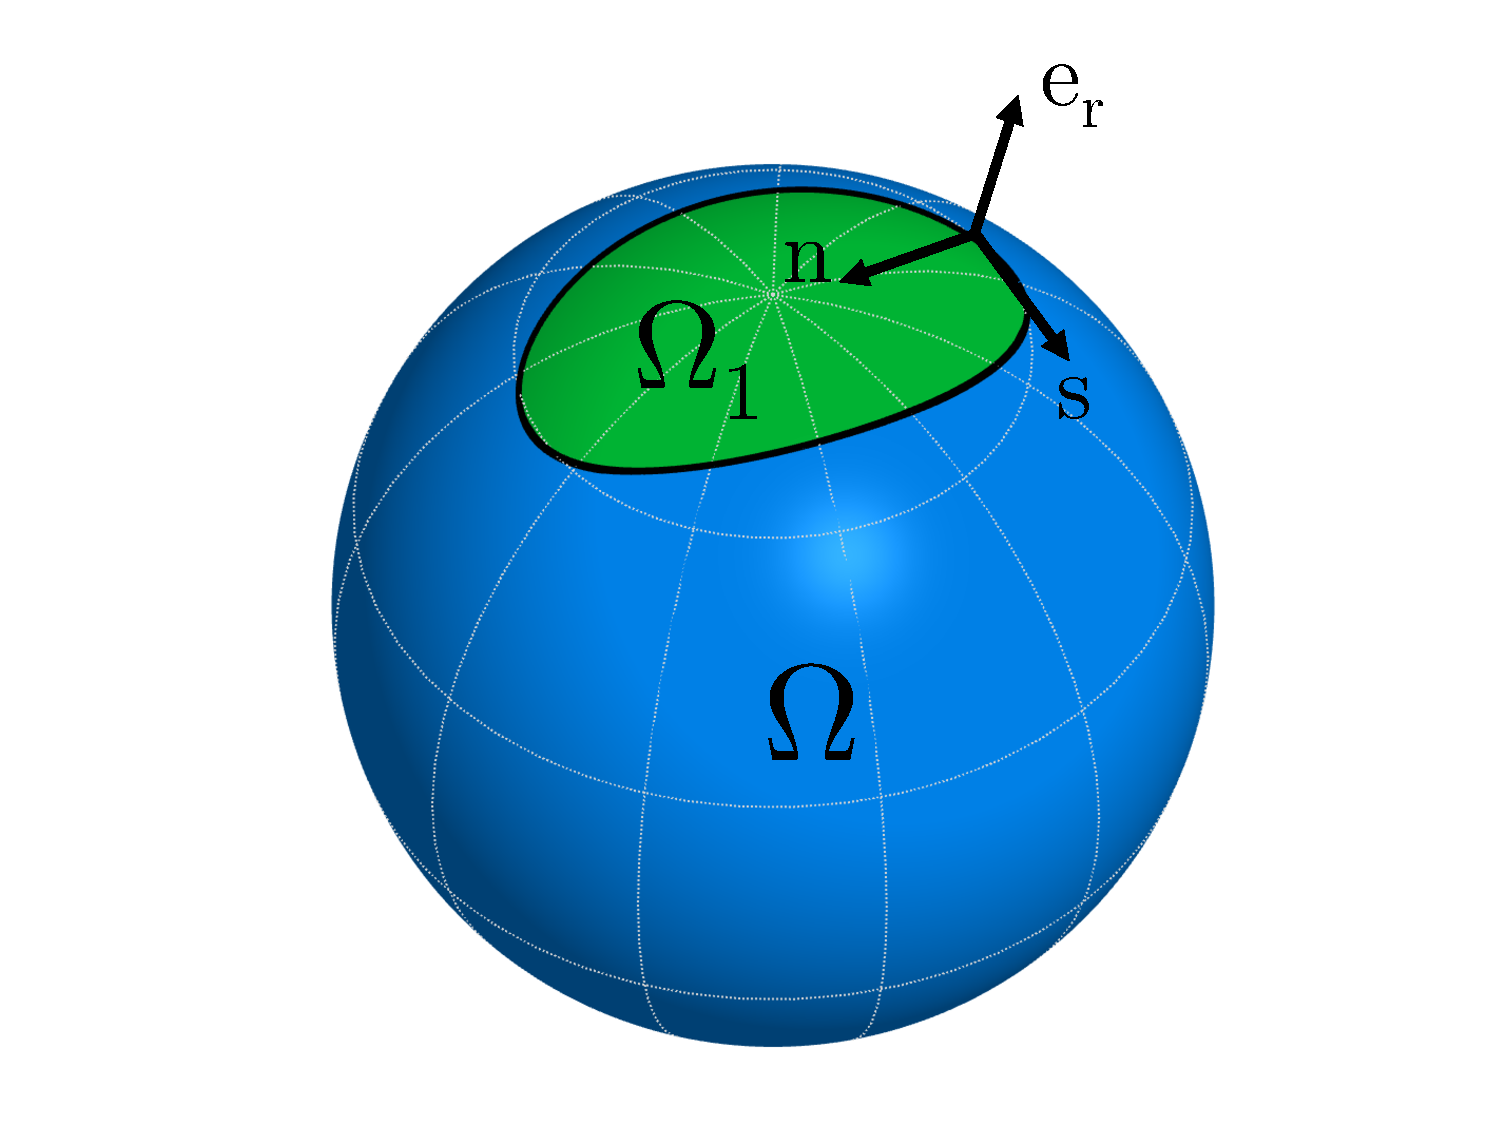
\includegraphics[width=0.35\textwidth]{SimplyConnectedDomain}
    	\caption{A simply connected domain, $\Omega$, on the surface of the sphere, $\mathcal{S}$, with a smooth, closed boundary $\Gamma$. The single island is denoted by ${\Omega}_1$. The normal, tangent and radial vectors are denoted by $\mathbf{n}$, $\mathbf{s}$ and ${\mathbf{e}}_r$ respectively. The normal vector, defined as $\mathbf{n}=\mathbf{s}\times{\mathbf{e}}_r$, points out of the domain $\Omega$ and is tangent to the surface of the sphere $\mathcal{S}$.}
   	\label{fig: SimplyConnectedDomain}
\end{figure}

Although we will work mostly with real Cartesian co-ordinates on the sphere, the initial discussion of the Laplace-Beltrami operator is easily expressed in spherical coordinates. A point $\mathbf{x} \in \mathcal{S}$ on the sphere can be described in the following way, 
\begin{align*}
	\mathbf{x}(\theta, \phi)=\begin{bmatrix} \sin\theta\cos\phi \\
                                                              \sin\theta\sin\phi \\
                                                              \cos\theta
                                                              \end{bmatrix}, \quad \theta \in [0,\pi], \phi \in [0, 2\pi).
\end{align*}
\noindent The unit vectors for the coordinate axes in the $\theta$ and $\phi$ direction are denoted by ${\mathbf{e}}_{\theta}$ and ${\mathbf{e}}_{\phi}$, respectively. The radial direction is represented by $\mathbf{e}_r$.  

To define the Laplace-Beltrami operator, we need to define the surface gradient on the sphere. Applied to a scalar field $f$ on $\mathcal{S}$, the surface gradient is given by 
\begin{align*}
	{\nabla}_\mathcal{S \ } f(\mathbf{x})= \frac{\partial f}{\partial \theta} {\mathbf{e}}_\theta + \frac{1}{\sin\theta}\frac{\partial f}{\partial \phi} {\mathbf{e}}_\phi . 
\end{align*}
The Laplace-Beltrami operator is then defined as the surface divergence of the surface gradient on the sphere, 
\begin{align*}
	\Delta_{\mathcal{S} \ } & \equiv \text{div}_S \nabla_{\mathcal{S}}, \\
                                    		& = \frac{1}{{\sin}^2\theta} \frac{{\partial}^2}{\partial \phi^2} + \frac{1}{\sin{\theta}} \frac{\partial}{\partial \theta} \left(\sin \theta \frac{\partial}{\partial \theta}\right).
\end{align*}

The Dirichlet boundary-value problem which we will be solving in this thesis is posed in the following way: \\
Find $u \in C^2(\bar{\Omega})$ such that 
\begin{align}
	\begin{split}
		{\Delta}_{\mathcal{S}\ }u(\mathbf{x})&=0,\\ 
		u(\mathbf{x})&=g(\mathbf{x}), \quad \mathbf{x} \in \Gamma. \label{eq: DirLapBelt}  
	\end{split}
\end{align}
Since $\Delta_{\mathcal{S}}$ is an elliptic operator, applying a BIE representation is a natural choice. The PDE posed on the subdomain of the sphere, $\Omega$, can be reformulated into an integral equation over the boundary, $\Gamma$, which reduces the dimension of the problem from two to one. Once a numerical scheme is applied, only the boundary needs to be discretized as opposed to the whole solution domain. Thus the resulting linear system is much smaller. 
The boundary integral reformulation also has advantages in cases of complicated geometry. In this thesis we consider only smooth boundaries, and as long as a parametric representation for the curve $\Gamma$ is provided, the solution can be found for any arbitrary, smooth shape. 

In addition, discretizing the BIE with the Nystr\"{o}m method, based on the trapezoidal rule, leads to superalgebraic convergence for smooth data on smooth, closed, and separated boundaries \cite{Atk97, Kress99}. Such a linear system is well-conditioned and its solution can be accelerated via the FMM or a fast direct solver. In some cases, as will be discussed in Chapter \ref{three}, the condition number of the linear system can grow if the boundary is not well-separated. However the condition number will still remain bounded independent of the size of the system. For the FMM, larger condition numbers often require more iterations for convergence, while for fast direct solvers, boundaries that are \enquote{close-to-touching} often require a large number of recursive levels in order to keep near field contributions local. 

This chapter first summarizes the steps for obtaining the boundary integral formulation on the surface of the sphere, based on previous work by \cite{GemmNigStein2008} and \cite{KropNig2014}. We also follow this by discussing how the Laplace-Beltrami can be mapped to the stereographic plane, which will prove useful when comparing our results with previous work. Details of the discretization are then given, along with the resulting properties of the linear system. 

% SECTION 2.1 -------------------------------------------------------------------------------------------------------------------------------------------------------------------------------------------
\section{The Generalized Fundamental Solution on the Sphere}
\label{sec: GenFundSoln}
To obtain a boundary integral reformulation of the BVP (\ref{eq: DirLapBelt}), we first need to obtain what is referred to as the \textit{generalized fundamental solution} for the Laplace-Beltrami equation on the sphere. This process is most easily explained through the application of point vortex motion which we will discuss in detail in Chapter \ref{five}. The motion of steady, incompressible fluid over the entire sphere $\mathcal{S}$ generated by a point vortex located at $\mathbf{x}_0 \in \mathcal{S}$ is described by a stream function $G(\mathbf{x},\mathbf{x}_0)$, $\mathbf{x} \in \mathcal{S}$. The velocity field of the fluid is given by 
\begin{align*}
	\mathbf{v}=\nabla G \times \text{e}_\mathbf{r},
\end{align*} 
and the vorticity field by 
\begin{align*}
	\bm{\omega}=\nabla \times \mathbf{v}=\left(-\Delta_{\mathcal{S}\ } G \right)\mathbf{e}_\mathbf{r}=\omega(\mathbf{x}, \mathbf{x}_0) \mathbf{e}_\mathbf{r}.
\end{align*}
The dynamics of the fluid are generated by a delta singularity, $\kappa \delta(\mathbf{x}-\mathbf{x}_0)$, in the vorticity field where $\kappa$ denotes the circulation induced by the vortex. 
In addition, since the sphere, $\mathcal{S}$, is a smooth, oriented surface, Stokes theorem places an additional constraint on the vorticity field, requiring that it integrates to zero over the spherical surface, i.e. 
\begin{align}
	\int_\mathcal{C} \mathbf{v} \cdot d\mathbf{r}=\int_\mathcal{S} \omega(\mathbf{x}, \mathbf{x}_0) ds_\mathbf{x} =0.  \label{eq: GaussConstraint} 
\end{align}
This property widely cited as the Gauss constraint \cite{Crowdy2006, Newt2001, Drit15, Crowdy2003, GemmNigStein2008}, requires that the generalized fundamental solution, or stream function, $G$ satisfy
\begin{align}
	-{\Delta}_{\mathcal{S} \ } G(\mathbf{x}, {\mathbf{x}}_0) = \kappa \left(\delta(\mathbf{x}-{\mathbf{x}}_0) - \frac{1}{4\pi}\right), \quad \mathbf{x} \in \mathcal{S}. \label{eq: GenFundSolnEqn} 
\end{align}
Thus the vorticity field on $\mathcal{S}$ given by the right hand side of (\ref{eq: GenFundSolnEqn}) represents a point vortex, denoted by the delta distribution, moving in a \enquote{sea} of uniform vorticity equal to $\frac{1}{4\pi}$. The constant $\frac{1}{4\pi}$ ensures the Gauss constraint is satisfied. 

The Gauss constraint is analogous to the compatibility condition imposed on Poisson's equation over a periodic domain in 2D. For example, in a periodic domain, $\Omega$, a stream function $\phi$ satisfying 
\begin{align*}
	-\Delta \phi = \omega(\mathbf{x}, \mathbf{x}_0), \quad \mathbf{x} \in \Omega
\end{align*}
also results in the same constraint (\cite{Gock2010}) after applying the divergence theorem, 
\begin{align*}
	\int_{\Omega} \omega(\mathbf{x}, \mathbf{x}_0) \ dx = \int_{\Omega} \Delta \phi \  dx = \int_{\partial \Omega} \frac{\partial \phi}{\partial n}  \ ds_{\mathbf{x}} =0.
\end{align*}

One possible way of obtaining the generalized fundamental solution which satisfies (\ref{eq: GenFundSolnEqn}), is to map the surface of the sphere to the stereographic plane, as will be shown in Section \ref{sec: StereographicProjection}. Under a stereographic projection, the Laplace-Beltrami operator becomes a variable coefficient elliptic operator in the complex plane \cite{KropNig2014}. Analogous to the fundamental solution for Laplace's equation in 2D, the fundamental solution to this variable coefficient operator also has a logarithmic singularity in the complex plane \cite{Crowdy2006, GemmNigStein2008}. 
Mapping back to real coordinates gives 
\begin{align}
	G(\mathbf{x},\mathbf{x_0})=-\frac{1}{2\pi}\log||\mathbf{x}-{\mathbf{x}}_0||+\frac{1}{4\pi}\log2. \label{eq: GenFundSoln}
\end{align}
On the sphere, this logarithmic singularity depends on the Euclidean, or chord distance between $\mathbf{x}$ and $\mathbf{x}_0$, denoted by $||\mathbf{x}-{\mathbf{x}}_0||$ \cite{Drit15, GemmNigStein2008}. As a result the generalized fundamental solution has the same form as in the plane, allowing many integral equation methods used in 2D to be extended to the sphere, as will be discussed throughout the thesis. 
However this is generally not as straightforward for other closed surfaces. Further details can be found in \cite{Drit15, Boatto2008}.

% SECTION 2.2 -------------------------------------------------------------------------------------------------------------------------------------------------------------------------------------------
\section{Boundary Integral Equation Formulation}
\label{sec: BIEFormulation}
There are several possible methods for reformulating the Laplace-Beltrami PDE (\ref{eq: DirLapBelt}) as an integral equation. We follow \cite{GemmNigStein2008, KropNig2014} and use an indirect approach using a layer ansatz. To motivate this approach we first look at Green's representation formula for a harmonic function on the surface of the sphere, which has the form, 
\begin{align}
	u(\mathbf{x})=\frac{1}{4\pi}\iint_{\Omega}u(\mathbf{x'})dS'-\int_{\Gamma}\left(u{\nabla}_S'G-G{\nabla}_S'u\right)\cdot \mathbf{n'}ds'.  \label{eq: GreensRepFormula}  
\end{align}
Here, $u$ satisfies ${\Delta}_{\mathcal{S}\ }u=0$, and $G(\mathbf{x},\mathbf{x'})$ is taken to be the fundamental solution on the surface of the sphere (\ref{eq: GenFundSoln}). The normal vector $\mathbf{n}'$, at the point $\mathbf{x'}\in \Gamma$, is tangent to the surface, and points out of the domain, $\Omega$ (Figure \ref{fig: SimplyConnectedDomain}). Also, the prime notation refers to differentiation or integration with respect to $\mathbf{x'}$. This formula follows from substituting $u$ and $G$ into Green's second identity, and taking appropriate limits. The derivation of Green's identities on the sphere and the representation formula are proved in \cite{GemmNigStein2008}. 

Equation (\ref{eq: GreensRepFormula}) shows that the solution to the Laplace-Beltrami equation, $u$, can be written as the sum of a single and double layer potential (defined below) and a constant which comes from the double integral of $u$ over $\Omega$ \cite{GemmNigStein2008}. This extra constant arises as a result of the Gauss constraint, which follows from the fact that we are working on a closed and bounded domain.  

The single and double layer potentials are defined as follows. For sufficiently smooth density functions $\rho$ and $\sigma$, the single layer has the form
\begin{align*}
	(V\rho)(\mathbf{x}) \coloneqq \int_\Gamma \rho(\mathbf{x'})G(\mathbf{x},\mathbf{x'})ds',
\end{align*}
and the double layer has the form 
\begin{align}
	(W\sigma)(\mathbf{x})&\coloneqq -\int_{\Gamma} \sigma(\mathbf{x'}){\nabla}_S' G(\mathbf{x},\mathbf{x'}) \cdot \mathbf{n'}ds' \nonumber \\
					      &=\frac{1}{2\pi}\int_{\Gamma}\sigma(\mathbf{x'})\frac{\partial}{\partial n'}\log||\mathbf{x}-\mathbf{x'}|| ds'. \label{eq: DLP} 
\end{align}

Either the single or double layer potential can be used to obtain an integral equation. The double layer potential is advantageous since it automatically satisfies the Laplace-Beltrami equation. The single layer potential, on the other hand, must satisfy an additional constraint on the density $\rho$, before it is a solution to the equation. This extra constraint is again due to the Gauss constraint on the sphere \cite{GemmNigStein2008}.  

In addition, as will be shown below, using the double layer potential leads to a Fredholm integral equation of the second kind that has a continuous, compact kernel \cite{KropNig2014}. Second kind integral equations lead to well conditioned matrices, which have bounded condition numbers independent of the number of discretization points, $N$ \cite{Atk97}. This means that iterative solvers perform well on these types of systems, and acceleration strategies like the FMM or fast direct solvers can be applied to achieve $O(N)$ time complexity. 

As a result, the double layer potential is chosen in this case. Since it satisfies the Laplace-Beltrami equation in $\Omega$, we are left with the boundary condition, $u=g(\mathbf{x}), \mathbf{x}\in \Gamma$, to satisfy in (\ref{eq: DirLapBelt}). For smooth curves, it is shown in \cite{GemmNigStein2008} that the double layer potential satisfies the following jump relation, 
\begin{align}
	\displaystyle \lim_{\substack{\mathbf{x}\to\mathbf{x'}\\ \mathbf{x}\in\Omega}}  (W\sigma)(\mathbf{x'})=\frac{1}{2}\sigma(\mathbf{x})+\frac{1}{2\pi}\int_{\Gamma}\sigma(\mathbf{x'})		\frac{\partial}{\partial n'}\log ||\mathbf{x}-\mathbf{x'}||ds'. \label{eq: JumpCondition} 
\end{align}
Applying the boundary condition for $u$, we obtain the following integral equation for $\sigma$, 
\begin{align}
	\frac{1}{2}\sigma(\mathbf{x})+\frac{1}{2\pi}\int_{\Gamma}\sigma(\mathbf{x'})\frac{\partial}{\partial n'}\log ||\mathbf{x}-\mathbf{x'}||ds'=g(\mathbf{x}). \label{eq: LB_BIE} 
\end{align}
We note that this BIE has the same form as for the planar problem in 2D. Consequently much of the theory and numerical techniques from 2D carry over to the sphere.

Since the boundary $\Gamma$ is smooth, the kernel, $K$ in (\ref{eq: LB_BIE}) given by 
\begin{align*}
	K\equiv \frac{\partial}{\partial n'} \log {||\mathbf{x}-\mathbf{x}'||} 
\end{align*}
is shown to be continuous along $\Gamma$ in \cite{KropNig2014} with 
\begin{align*}
	\lim_{\substack{\mathbf{x}\to\mathbf{x'}\\ \mathbf{x}\in\Gamma}} \frac{\partial}{\partial n'}\log||\mathbf{x}-\mathbf{x'}||=\frac{1}{2}\mathbf{s}\cdot(\kappa\mathbf{N_p}\times \mathbf{x}).
\end{align*}
Here, $\mathbf{s}$ is the tangent vector at the point $\mathbf{x}$, $\kappa$ denotes the curvature at $\mathbf{x}$, and $\mathbf{N_p}$ denotes the principal normal.  

If $\sigma$ satisfies (\ref{eq: LB_BIE}), then $u=(W\sigma)(\mathbf{x})$ solves (\ref{eq: DirLapBelt}). Hence, solving  (\ref{eq: LB_BIE}) for $\sigma$ and evaluating $u=(W\sigma)(\mathbf{x})$, gives the solution to (\ref{eq: DirLapBelt}) throughout $\Omega$. 

Equation (\ref{eq: LB_BIE}) is a Fredholm integral equation of the second kind. Since it has a continuous kernel, it is compact.  Furthermore, the null space of $(I+K/ \pi) \sigma=0$ is trivial, so we can apply the Fredholm Alternative Theorem \cite{Atk97}, which states that the integral equation (\ref{eq: LB_BIE}) has a unique solution for any integrable boundary data $g$. 

% SECTION 2.3 -------------------------------------------------------------------------------------------------------------------------------------------------------------------------------------------
\section{The Stereographic Projection}
\label{sec: StereographicProjection}
The BVP in (\ref{eq: DirLapBelt}) can be equivalently posed in the complex plane by applying a stereographic projection to the surface of the sphere. Many authors \cite{KropNig2014, Crowdy2006, Kid2000, Kid2000Stream, Newt2001} work with the equation in this form since analogies can be drawn with the 2D planar problem and complex variable theory can be exploited to find solutions. Although we work almost exclusively in real Cartesian co-ordinates, we will occasionally refer to the Laplace-Beltrami equation posed in the stereographic plane, especially when applying past results in this area. We also plot many of our numerical examples in the stereographic plane since the behaviour of the solutions over the entire surface can be viewed in a flat plane. In this section we introduce the stereographic projection, summarizing the details given in \cite{KropNig2014, Crowdy2006}. 

For a point $\mathbf{x}=(x, y, z) \in \mathcal{S}$, the stereographic projection is given by 
\begin{align}
	\xi = \cot \left(\frac{\theta}{2}\right) e^{i\phi} = \frac{x+iy}{1-z}, \quad \xi \in \mathbb{C}. \label{eq: Sphere2Stereo}
\end{align}
The mapping from the complex plane back to the sphere is given by
\begin{align}
	x=\frac{\xi + \bar{\xi}}{1+ {|\xi|}^2}, \quad y=\frac{\xi - \bar{\xi}}{i(1+{|\xi|}^2)}, \quad z=\frac{1-{|\xi|}^2}{1+{|\xi|}^2} \label{eq: Stereo2Sphere}.
\end{align}
The stereographic projection maps the north pole, $\mathbf{x}= (0,0,1)$ to infinity, while the south pole is mapped to the origin and the equator to the unit circle. For a simply connected domain $\Omega$, we can assume without loss of generality that the island $\Omega_1$ is placed over the north pole \cite{KropNig2014}. The domain $\Omega$, is then mapped to a bounded region in the complex plane denoted by $\tilde{\Omega}$. Likewise we denote the stereographic projections of $\Gamma$ and $\Omega_1$ as $\tilde{\Gamma}$ and $\tilde{\Omega}_1$, respectively. An example of a stereographic projection of a simply connected domain is shown in Figure \ref{fig: SimplyConnectedStereo}. 

Applying the stereographic mapping (\ref{eq: Sphere2Stereo}) to the Laplace-Beltrami operator gives
\begin{align*}
	\Delta_{\mathcal{S} \ } \equiv {(1+{|\xi|}^2)}^2\frac{{\partial}^2}{\partial_{\xi \bar{\xi}}}= {(1+{|\xi|}^2)}^2 \ \Delta, 
\end{align*} 
where $\Delta$ is the Laplace operator on the plane. Therefore, harmonic functions in the plane will satisfy the Laplace-Beltrami equation on the sphere under stereographic projection. Thus exact solutions in the stereographic plane can be used to generate exact solutions on the sphere. We use this approach to generate test cases for many of the numerical examples presented later in this thesis. 

The BVP (\ref{eq: DirLapBelt}) can be rewritten as, 
\begin{align*}
	-\Delta_{\mathcal{S}\ } \psi(\xi, \xi_0)&=0,  \quad \xi \in \tilde{\Omega}\\
\psi(\xi)&=g(\mathbf{x}(\xi)) \quad \xi \in \tilde{\Gamma}.
\end{align*} 

Mapping the generalized fundamental solution from the sphere to the complex plane, gives \cite{SurCrow2008}  
\begin{align*}
	G(\xi, \xi_0)=-\frac{1}{4\pi} \log \left(2 \frac{(\xi -\xi_0)-(\bar{\xi}- \bar{\xi}_0)}{(1+{|\xi|}^2)(1+{|\xi_0|}^2)}\right).
\end{align*}
Doing the same for the double layer potential gives \cite{KropNig2014} 
\begin{align*}
	(W\sigma)(\xi)=\text{Re}\left\{\frac{1}{2\pi i}\int_{\tilde{\Gamma}} \sigma(\xi ')\left[\frac{1}{\xi -\xi '} - \frac{\bar{\xi} ' }{1+ {|\xi '|}^2}\right] d\xi ' \right\}, \quad \xi \in \tilde{\Omega},
\end{align*}
which leads to the BIE, \cite{KropNig2014}
\begin{align*}
	\frac{1}{2}\sigma(\xi)+\text{Re}\left\{\frac{1}{2\pi i}\int_{\tilde{\Gamma}} \sigma(\xi ')\left[\frac{1}{\xi -\xi '} - \frac{\bar{\xi} ' }{1+ {|\xi '|}^2}\right] d\xi ' \right\}= g(\mathbf{x}(\xi)), \quad \xi \in \tilde{\Gamma}. 
\end{align*}
Thus taking a BIE approach on the sphere in $\mathbb{R}^3$ or in the stereographic plane will give equivalent solutions. 

\begin{figure}[h]  
	\centering
	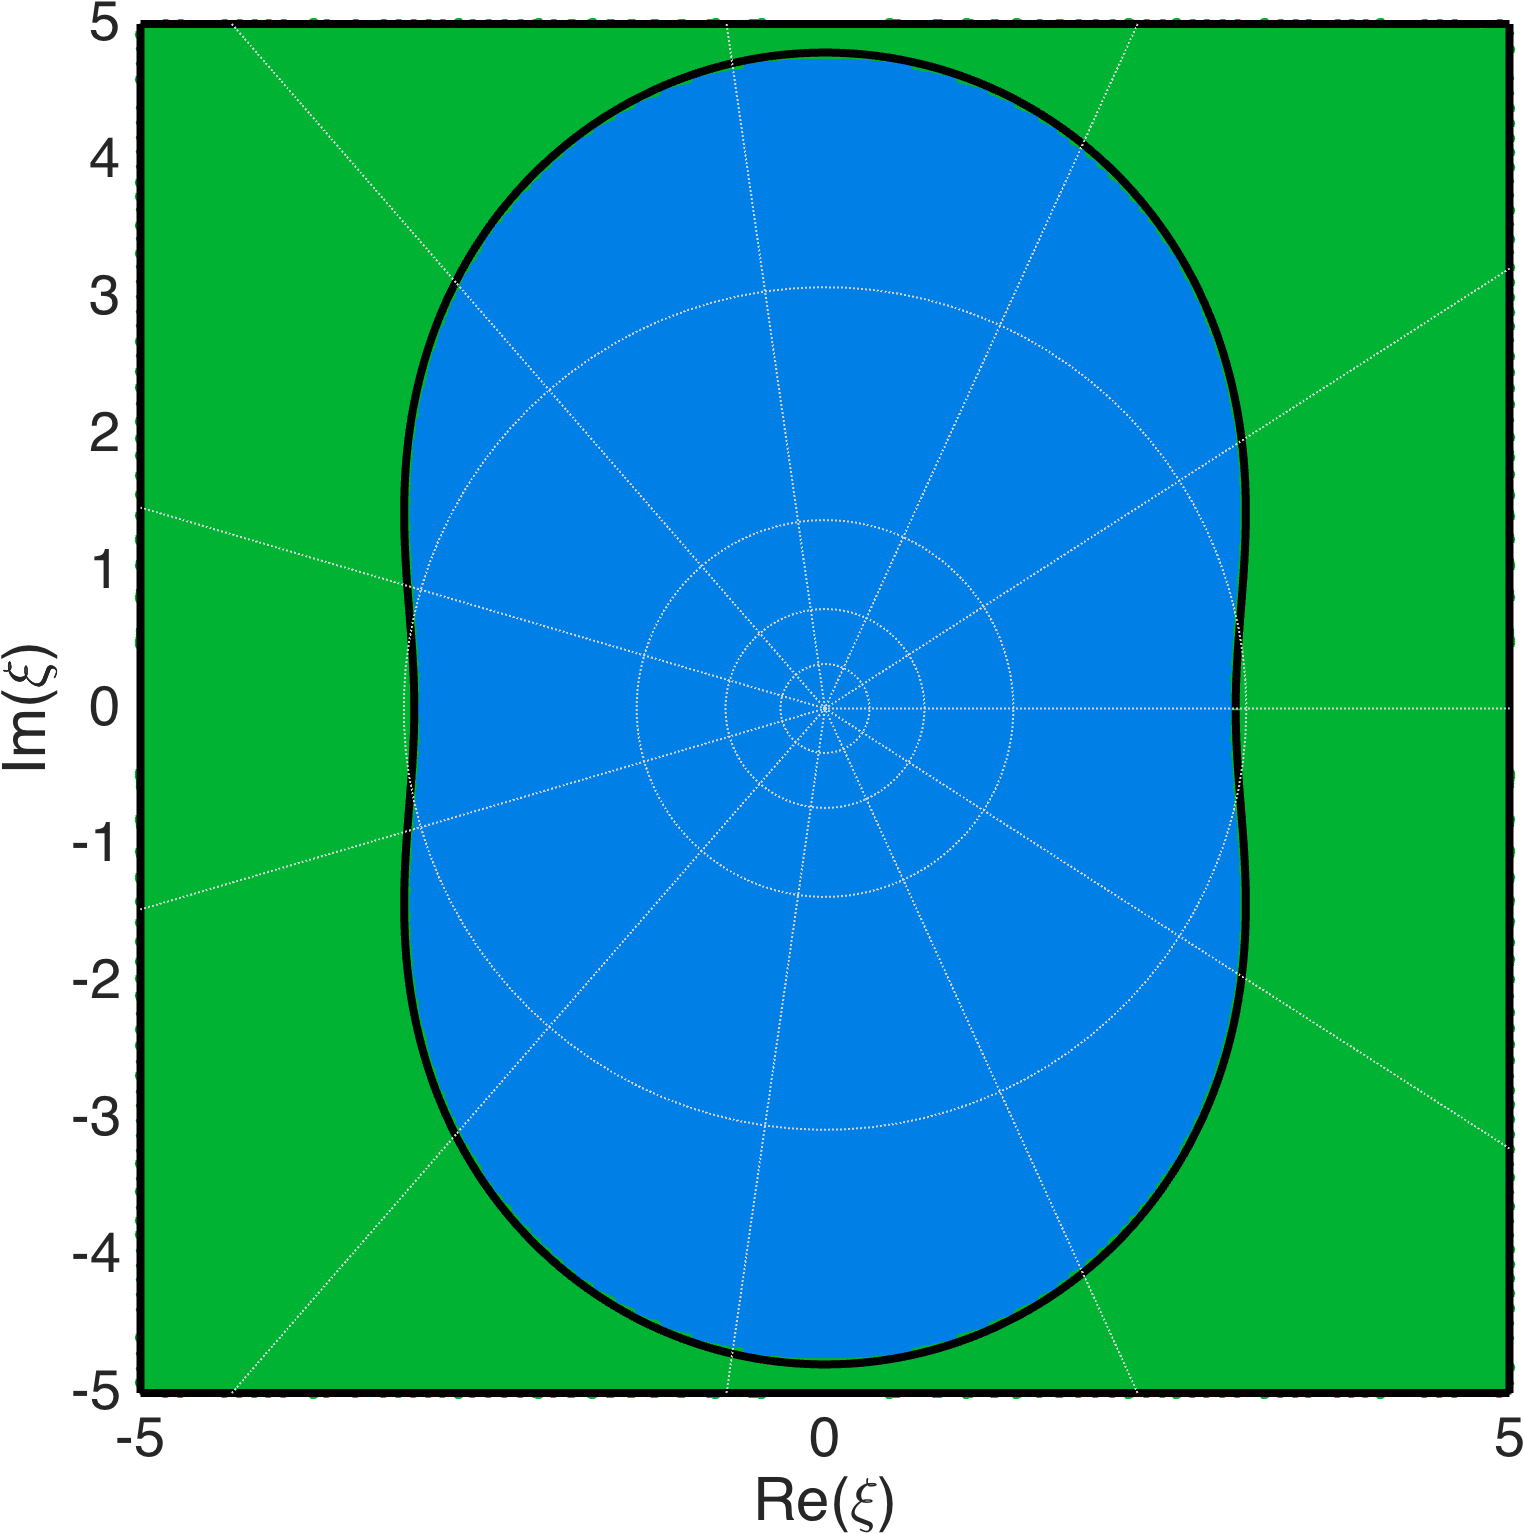
\includegraphics[width=0.5\textwidth]{SimplyConnectedStereo}
	\caption{The simply connected domain from Figure \ref{fig: SimplyConnectedDomain} mapped to the stereographic plane. }
	\label{fig: SimplyConnectedStereo}
\end{figure}

% SECTION 2.4 -------------------------------------------------------------------------------------------------------------------------------------------------------------------------------------------
\section{Nystr\"{o}m Method}
\label{sec: Nystrom}
Returning to the BIE posed in real coordinates on the sphere (\ref{eq: LB_BIE}), we now examine how a numerical solution for the Laplace-Beltrami equation can be obtained. The Nystr\"{o}m Method with the trapezoid rule is used to discretize the integral equation since it gives super-algebraic convergence for smooth data on smooth, closed, boundaries \cite{Atk97, Kress99}. 

Given a parametric description of the boundary, oriented clockwise as in Figure \ref{fig: SimplyConnectedDomain}, 
\begin{align*}
	\mathbf{r}(t)=(r_1(t), r_2(t), r_3(t)), \quad t\in\left[0,2\pi\right),
\end{align*}
the curve is discretized into $N$ grid points, equi-spaced in $t$. The integral in (\ref{eq: LB_BIE}) is approximated by the trapezoid rule, 
\begin{align}
	\sigma(t)+\frac{h}{\pi}\sum_{j=1}^NK(\mathbf{r}(t),\mathbf{r}_j)\sigma_j=2g(t), \quad t\in\left[0,2\pi\right), \label{eq: NIF}
\end{align}
where $h=\frac{2\pi}{N}$, $t_j=jh$, $\mathbf{r}_j=\mathbf{r}(t_j)$, and ${\sigma}_j=\sigma(\mathbf{r}(t_j))$. 
Then $\sigma(t)$ and $g(t)$ are evaluated at the node points, 
\begin{align}
	{\sigma}_i+\frac{h}{\pi}\sum_{j=1}^NK(\mathbf{r}_i, \mathbf{r}_j){\sigma}_j=2g_i, \quad i=1,...,N, \label{eq: NystSystem} 
\end{align}
where 
\begin{align*}
	K(\mathbf{r}_i, \mathbf{r}_j)=\begin{cases} 
      		-\frac{(\mathbf{r}_i-\mathbf{r}_j)\cdot\mathbf{n}_j}{{||\mathbf{r}_i-\mathbf{r}_j||}_2^2}ds_j & i\neq j \\
      		\frac{1}{2}\mathbf{s}_i\left(\left(\kappa \mathbf{N_p}\right)_i \times \mathbf{r}_i\right)ds_i & i=j .
        \end{cases}
\end{align*}
Here, $\mathbf{n}_i=\mathbf{n}(t_i)$, and the same holds for the remaining vectors. Also, 
\begin{align*}
	ds_j={\left|\frac{d\mathbf{r}}{dt}\right|}_j. 
\end{align*}
The normal and principal normal vectors are given by
\begin{align*}
	\mathbf{n}_i=(\mathbf{s}_i\times \mathbf{r}_i), \quad \left(\kappa \mathbf{N}_{p}\right)_i=\frac{1}{ds_i} \left.\frac{ds}{dt} \right|_{t_i}, 
\end{align*}
where $s$ is arc length. 

Equation (\ref{eq: NystSystem}) gives a dense linear system for $\bm{\sigma}={(\sigma_1,\sigma_2,...,\sigma_N)}^T$, of the form 
\begin{align}
	\left(I+\frac{1}{\pi}K\right)\bm{\sigma}=2\mathbf{g}, \text{ or } A\bm{\sigma}=\mathbf{b}, \label{eq: LBSystem} 
\end{align}
where $\mathbf{g}={(g_1, g_2, ..., g_N)}^T$. 
Numerical strategies for solving this system are discussed in the next chapter.

We note that equation (\ref{eq: NIF}) provides an interpolation formula to evaluate $\sigma(t)$ anywhere along the curve $\Gamma$. It is referred to as the \textit{Nystr\"{o}m Interpolation Formula} \cite{Atk97}.

Also, \cite{Atk97} and \cite{Kress99} show that if the true solution is denoted by $\widetilde{\sigma}$, then ${||\widetilde{\sigma}-{\sigma}||}_\infty \to 0$, as $N\to\infty$ at the same rate as the quadrature scheme chosen. In this case we obtain super-algebraic convergence with the trapezoid rule, which can be shown using the Euler-Maclaurin formula \cite{Greenbaum12}. In 2D, when $\mathbb{R}^2$ can be associated with the complex plane, a bounded and analytic function over a closed boundary can be shown to achieve exponential convergence \cite{Barn14}. This connection with analytic functions cannot be made in 3D, however we can numerically verify that the trapezoidal rule gives not only super-algebraic convergence, but exponential convergence in many cases.  

Once we have $\sigma$, we can use it to find the approximate solution, $u(\mathbf{x})$, to the original problem (\ref{eq: DirLapBelt}), for any point $\mathbf{x} \in \Omega$. Typically, the Nystr\"{o}m interpolation formula is not used, and $u$ is evaluated using the same quadrature rule and grid points as the integral equation. The approximate solution is given by
\begin{align}
	u(\mathbf{x})=\frac{h}{2\pi}\sum_{j=1}^N K(\mathbf{x},\mathbf{r}_j)\sigma_j ds_j, \quad \mathbf{x}\in \Omega. \label{eq: DiscreteRepFormula}
\end{align}

Atkinson \cite{Atk97} shows that the speed of convergence of the approximate solution is also comparable to the speed of the quadrature rule, as long as $\mathbf{x}$ is evaluated away from the boundary. Typically $\mathbf{x}$ is chosen to be a distance of $5h$ from the boundary. This is rigorously shown for 2D domains in \cite{Barn14}, but has not yet been proven in 3D, although it has been verified empirically. Evaluating $u(\mathbf{x})$ up to the boundary is known as the close evaluation problem and is studied in \cite{Klock13, Barn14, Hels08}. 

%   CHAPTER 3  %%%%%%%%%%%%%%%%%%%%%%%%%%%%%%%%%%%%%%%%%%%%%%%%%%%%%%%%%%%%%%%%%%%%%%%
\chapter{Fast Direct Solvers}
\label{three}

The focus in this thesis is on the solution of the linear system (\ref{eq: LBSystem}), which arises from the Nystr\"{o}m discretization of the BIE for the Laplace-Beltrami Equation. Although the integral equation strategy leads to matrices of smaller dimension than other approaches, the matrices are dense. For complicated domains that require a very fine grid along the boundary, solving the system with $N$ unknowns with a standard Gaussian elimination scheme of $O(N^3)$ is prohibitively expensive. 

To accelerate the solution of the linear system, we can take an iterative or direct approach. Iterative approaches such as GMRES, conjugate gradient or Gauss-Seidel, start with an initial guess and then successively construct a sequence of solutions which converge to some preset tolerance. For linear systems arising from BIEs for elliptic PDEs, combining iterative methods with the landmark fast multipole method (FMM) to accelerate matrix vector products allows systems to be solved in $O(N)$ operations \cite{GreenRok87, Green88}. This approach has been used for several decades and provides some of the fastest and most accurate solvers known today \cite{HoGreen2012}. 

Direct methods on the other hand, like the LU decomposition, produce an exact solution up to round-off error in a finite number of operations. Up until recently, they have been considered too computationally expensive to be used in practical applications. However, the development of fast direct solvers for BIEs from elliptic PDEs has brought attention back to these types of methods. They achieve $O(N)$ complexity in 2D and present a favourable alternative to the FMM specifically for problems involving multiple right hand sides, or for matrices with ill-conditioning arising from the geometry of the problem \cite{MartRokh2005, GillYoungMart2012, HoGreen2012}. 

Both iterative and direct solvers have been extensively studied in the context of elliptic PDEs posed in two and three dimensions, but less so for PDEs posed on surfaces. For the first time in \cite{KropNig2014}, Kropinski and Nigam apply an iterative method to solve the BIE arising from the Laplace-Beltrami equation on the surface of the sphere, confirming that $O(N)$ complexity can be achieved with the FMM. 

Direct solvers, however, have not been applied to PDEs posed on surfaces to date. In this thesis we use the same integral formulation presented in \cite{KropNig2014}, and develop a fast direct solver for the Laplace-Beltrami equation on the sphere. This solver is based on the extensive literature for solvers in 2D and 3D (\cite{MartRokh2005, GillYoungMart2012, HoGreen2012} to name just a few). We outline the specific changes that need to be made to adapt the solvers to a surface, and we verify that $O(N)$ complexity can be achieved, just as in the plane. 

We first give a brief overview of iterative and direct solvers in the following two sections, including the advantages and disadvantages of each approach. 

%--------------------------------------------------------------------------------------------------------------------------------------------------------------------------------------------------------------------------------------

\subsubsection{Iterative Methods}

In the numerical solution of elliptic PDEs, iterative methods are the standard approach for solving large, sparse, linear systems which arise from finite difference discretizations, and other similar discretization schemes \cite{Lev2007}. With the development of numerical approaches for solving integral equations, iterative methods have also been adapted to deal with the dense linear systems arising from this context. To solve a system like (\ref{eq: LBSystem}), iterative methods access matrix elements through matrix-vector products, i.e.  $(I+K/ \pi)\bm{\sigma}$. As mentioned above, they construct a sequence of approximations  $\bm{\sigma}_1,\bm{\sigma}_2, ...$, to the solution which converges to within some preset tolerance. BIE matrices based on a double layer potential formulation are non-symmetric. Hence GMRES is typically used to solve such a system, which is a Krylov subspace method \cite{Tref97}.

There are two factors affecting the computation time for an iterative solution of a linear system: The conditioning of the matrix, which influences the number of iterations required to achieve convergence, and the cost of matrix-vector products. 

Typically, the condition number will depend on $N$. For example, the condition number for a matrix associated with a finite difference method for a second order PDE is $O(N^2)$ \cite{Lev2007}. Therefore, as the grid over the solution domain is refined, the number of iterations increase. For Fredholm integral equations of the second kind, the condition number remains bounded independent of $N$ \cite{Atk97}. This means the number of iterations for convergence is fixed. It is possible that the the condition number can become large when contours are not well-separated or are "close to touching" \cite{HoGreen2012}. In this case the number of iterations can grow, increasing the computational cost of the iterative method. However the condition number and the number of iterations still remain fixed across $N$.

The cost of each iteration is determined by the cost of matrix-vector products. Direct matrix vector multiplication requires $O(N^2)$ operations. To decrease this, the  fast multipole method (FMM) is used \cite{CarrGreenRok88, Green88, GreenRok87}. This method was originally developed to evaluate potential fields arising from a system of $N$ charged particles. In the context of Laplace's equation, each matrix-vector product represents a gravitational or electrostatic potential arising from a summation over $N$ sources, or charges. When sources and targets are well-separated, a multipole expansion for the fundamental solution can be applied which allows groups of sources which lie close together to be treated as a single source. By employing a hierarchal, or recursive strategy on the solution domain, the FMM is able to reduce the cost of a matrix-vector multiply to $O(N)$. As a result the method has been widely used in the solution of elliptic boundary value problems. A thorough review is given in \cite{Nish2002}. 

As previously mentioned, Kropinski and Nigam \cite{KropNig2014} employ an FMM-accelerated iterative strategy to solve the Laplace-Beltrami equation on the surface of the sphere. They apply a stereographic projection, and map the domain to the complex plane. Here the kernel has a similar form to the 2D Coulomb potential. They then use GMRES, combined with the FMM for the 2D electrostatic potential to solve the integral equation, achieving $O(N)$ complexity. 

To solve the problem directly on the sphere in $\mathbb{R}^3$, a 3D FMM routine that works for the generalized fundamental solution to the Laplace-Beltrami equation would need to be developed. Another option would be to apply a kernel independent FMM \cite{Ying2004}. This would require adapting algorithms from 2D and 3D to the surface of the sphere.

However, these options still present a fundamental drawback to iterative approaches which is that they are  ill-suited for linear systems with multiple right hand sides. Each new right hand side is treated virtually as a new problem. This is problematic since many applications require the solution of a linear system with changing right hand sides. This includes applications which model time dependent processes in fixed geometries \cite{HoGreen2012}. For example, the motion of a point vortex on the sphere involves repeatedly solving the Laplace-Beltrami equation for each new vortex position. For these types of applications it becomes impractical to apply iterative solvers. 

%--------------------------------------------------------------------------------------------------------------------------------------------------------------------------------------------------------------------------------------

\subsubsection{Fast Direct Solvers}

Fast direct solvers, which have been developed more recently, overcome some of the drawbacks of iterative solvers. Given some computational tolerance, $\varepsilon$, and a linear system like (\ref{eq: LBSystem}), 
\begin{align}
	A\bm{\sigma}=\mathbf{b}, \label{eq: FDSSystem} 
\end{align}
the solvers construct a factorization that approximates $A$ such that 
\begin{align}
	||A-A_\varepsilon||<\varepsilon.  \label{eq: FDSCompression} 
\end{align}
As will be discussed in upcoming sections, $A_\varepsilon$ is built of multiple factors in which all but one are block diagonal. The remaining factor forms a compressed (or what is referred to as a "skeletonized") representation of $A$ \cite{ChengEtAl2005, MartRokh2005, GillYoungMart2012}. Due to the special form of these factors $A_\varepsilon$ is said to be in a "data-sparse" format. This data-sparse factorization can be obtained through a recursive algorithm which is essentially based on repeated applications of pivoted or rank-revealing QR. 

One can solve the system in this factored form,
\begin{align*}
	A_\varepsilon \bm{\sigma}=\mathbf{b},
\end{align*}
 or construct an operator $A_\varepsilon^{-1}$ such that
\begin{align}
	||A^{-1}-A_{\varepsilon}^{-1}||<\varepsilon. \label{eq: FDSInversion} 
\end{align}
The data-sparse factorization of $A_\varepsilon$ allows an inverse operator $A_\varepsilon^{-1}$ to be efficiently constructed, which can then be applied to the right hand side of (\ref{eq: FDSSystem}) to find an approximate solution,
\begin{align}
	\bm{\sigma}_\varepsilon=A_\varepsilon^{-1}\mathbf{b}. \label{eq: FDSSolution} 
\end{align}
As will be discussed in Section \ref{sec: SingLevel}, $A_\varepsilon^{-1}$ is also in a data-sparse format, which allows it to be quickly applied to the right hand side. Thus once the matrix $A$ is compressed and inverted, applying $A_\varepsilon^{-1}$ to the right hand side is extremely efficient, making this approach very suitable for problems with multiple right hand sides. Unlike iterative solvers, this solution process is also deterministic, in that it always produces a solution in a fixed number of steps \cite{MartRokh2005, GillYoungMart2012, HoGreen2012}.

For general matrices, the data-sparse format is achieved by compressing rank-deficient submatrices using a matrix factorization algorithm known as the Interpolative Decomposition (ID) \cite{ChengEtAl2005}. This factorization is based on rank-revealing or pivoted QR. Depending on the structure of the system, various gains in computational efficiency can be obtained. 

Matrices arising from a Nystr\"{o}m discretization of a BIE, like (\ref{eq: LBSystem}), have structured rank-deficient off-diagonal blocks. Once factored with the ID, these off-diagonal blocks can be rearranged to expose more rank deficiencies that can be recompressed, leading to a recursive algorithm. The cost of applying the ID to each off-diagonal block is determined from the cost of pivoted QR which depends on the rank and dimension of the block being compressed. Summing up this cost over all recursive levels will give a compression algorithm with time complexity $O(N^2)$. BIE matrices with such structured off-diagonal blocks are described as \textit{hierarchically block separable} in the fast direct solver literature \cite{GillYoungMart2012, HoGreen2012}. 

Matrices arising from BIEs such as Laplace's equation have the added property that they represent a discretized kernel which comes from a single or double layer potential. Similar to the FMM, the block low-rank structure can be understood in terms of far field interactions between groups of sources and targets \cite{HoGreen2012}. This implies that far field interactions can be approximated by a smaller set of equivalent sources or targets, resulting in off-diagonal blocks with smaller dimension. This reduces the cost of the QR and the subsequent cost of the ID, allowing the recursive $O(N^2)$ algorithm to be accelerated to $O(N)$. For fast direct solvers, it is the existence of a Green's theorem associated with the underlying PDE that enables this approximation of far field interactions to take place \cite{MartRokh2005, HoGreen2012}. With this added property, solvers can achieve $O(N)$ complexity, both for obtaining a factorization, as in (\ref{eq: FDSCompression}), and for computing the solution, (\ref{eq: FDSSolution}).

An advantage of direct solvers widely cited in literature is that the solution time of a fast direct solver is relatively insensitive to geometric ill-conditioning \cite{MartRokh2005, GillYoungMart2012, HoGreen2012}. In the case where an island is thin and elongated and/or where the boundary is "close-to-touching", or in the multiply connected case where several islands are close together, the condition number of the system can increase. With iterative methods, dealing with this issue usually means finding appropriate pre-conditioners for the system, whereas with direct solvers no changes need to be made.  

As previously mentioned, direct solvers have been developed for elliptic PDEs in 2D and 3D, however they have not been applied to problems on manifolds to date. This thesis adapts a 2D fast direct solver to the Laplace-Beltrami equation on surface of the sphere. We verify that since the boundary remains one-dimensional, and the double layer potential has the same form as in the plane, the cost of compression and solution remains $O(N)$. 

%--------------------------------------------------------------------------------------------------------------------------------------------------------------------------------------------------------------------------------------

\subsubsection{Outline of Chapter}

This chapter first summarizes some key ideas necessary to implement fast direct solvers on the sphere based on several papers from the fast direct solver community \cite{GillYoungMart2012, HoGreen2012, MartRokh2005, ChengEtAl2005}. We also draw from slides presented at the 2014 CBMS-NSF Conference on Fast Direct Solvers for Elliptic PDEs at Dartmouth College \cite{CBMS}. The block low rank structure of the system (\ref{eq: LBSystem}) is described first in Section \ref{sec: RankDeficientSystem}. Then in Section \ref{sec: ID} we introduce the ID and pivoted QR, which are the main tools which allow the off-diagonal blocks of (\ref{eq: LBSystem}) to be compressed. In Section \ref{sec: SingLevel} we describe how the ID is applied to the full system matrix (\ref{eq: LBSystem}) for a single level compression, or "skeletonization". The recursive procedure is explained in the following section, along with the resulting structure of the factorization. Since this process carries over from 2D onto the sphere with no significant changes, we discuss these steps directly in terms of the discretized integral equation on the sphere. 

We then discuss the acceleration of the recursive procedure by approximating far field interactions with so called \enquote{proxy points.} This process is first examined in detail for the planar, two dimensional case in Section \ref{sec: 2DProxy} and later extended to the surface of the sphere in the following section. The ability to extend proxy points to the surface of the sphere is the main reason why we are still able to achieve $O(N)$ complexity.

Lastly, once the compressed, or data-sparse, representation for the matrix is obtained, one option is to construct a compressed inverse like (\ref{eq: FDSInversion}), which is done in \cite{GillYoungMart2012, MartRokh2005}. However, we follow Ho and Greengard \cite{HoGreen2012} instead, and embed the compressed matrix, (\ref{eq: FDSCompression}) into a sparse matrix. We then use the sparse solver software, UMFPACK to factor and solve the system. This solution procedure has the same $O(N)$ cost as in 2D. UMFPACK provides an efficient LU decomposition of the sparse matrix which allows it to be cheaply applied to the right hand side. This solution process is discussed in Section \ref{sec: umfpack}. 

% SECTION 3.1 -------------------------------------------------------------------------------------------------------------------------------------------------------------------------------------------
\section{Rank-Deficient Structure of System}
\label{sec: RankDeficientSystem}
As mentioned above, a key feature of systems arising from the discretization of elliptic BIEs is that they have rank-deficient off-diagonal blocks \cite{ChengEtAl2005, MartRokh2005, Stein2007}. For the system (\ref{eq: LBSystem}) that we work with, which arises from the Dirichlet Laplace-Beltrami BVP (\ref{eq: DirLapBelt}), this low rank structure can be understood in terms of interactions between sources and targets along the boundary, $\Gamma$ \cite{ChengEtAl2005, MartRokh2005, HoGreen2012}. 

The matrix $K$ in the system (\ref{eq: LBSystem}) 
corresponds to the discretized double layer potential 
\begin{align*}
	K(\mathbf{x}, \mathbf{x}')\sigma(\mathbf{x'}) = \int_{\Gamma} \sigma(\mathbf{x}') \frac{\partial}{\partial n'} \log{||\mathbf{x}-\mathbf{x}'||} ds' , \quad \mathbf{x} \in \Gamma.
\end{align*}
$K\sigma$ then represents the electrostatic potential on $\Gamma$ due to dipole charges, $\frac{\partial}{\partial n'}\log||\mathbf{x}-\mathbf{x}'||$, distributed over the boundary with some density $\sigma$. 
Examining the potential over an arbitrary segment of the boundary $\Gamma_\tau$, given by 
\begin{align}
	K(\mathbf{x}, \mathbf{x}')\sigma(\mathbf{x}')=\int_\Gamma \sigma(\mathbf{x}') \frac{\partial}{\partial n'} \log{||\mathbf{x}-\mathbf{x}'||} ds' , \quad \mathbf{x} \in \Gamma_\tau, \label{eq: PotentialGammaTau} 
\end{align}
we can split the charges along $\Gamma$ into three parts \cite{CBMS} (Figure \ref{fig: SourcesSelfNearFar}): 
\begin{align*}
	\Gamma=\Gamma_{\text{self}} + \Gamma_{\text{near}} + \Gamma_{\text{far}}.
\end{align*}
$\Gamma_{\text{self}}$ represents the self-interaction charges on $\Gamma_\tau$, while $\Gamma_{\text{near}}$ and $\Gamma_{\text{far}}$ represent the near and far field sources lying on the remainder of the boundary. The sources on $\Gamma_{\text{self}}$ and $\Gamma_{\text{near}}$ have the largest contribution to the potential and cannot readily be reduced or approximated, while, on the other hand,  the far field charges decay \cite{ChengEtAl2005, MartRokh2005, HoGreen2012, Stein2007}. 

\begin{figure}[h]
  	\centering
   	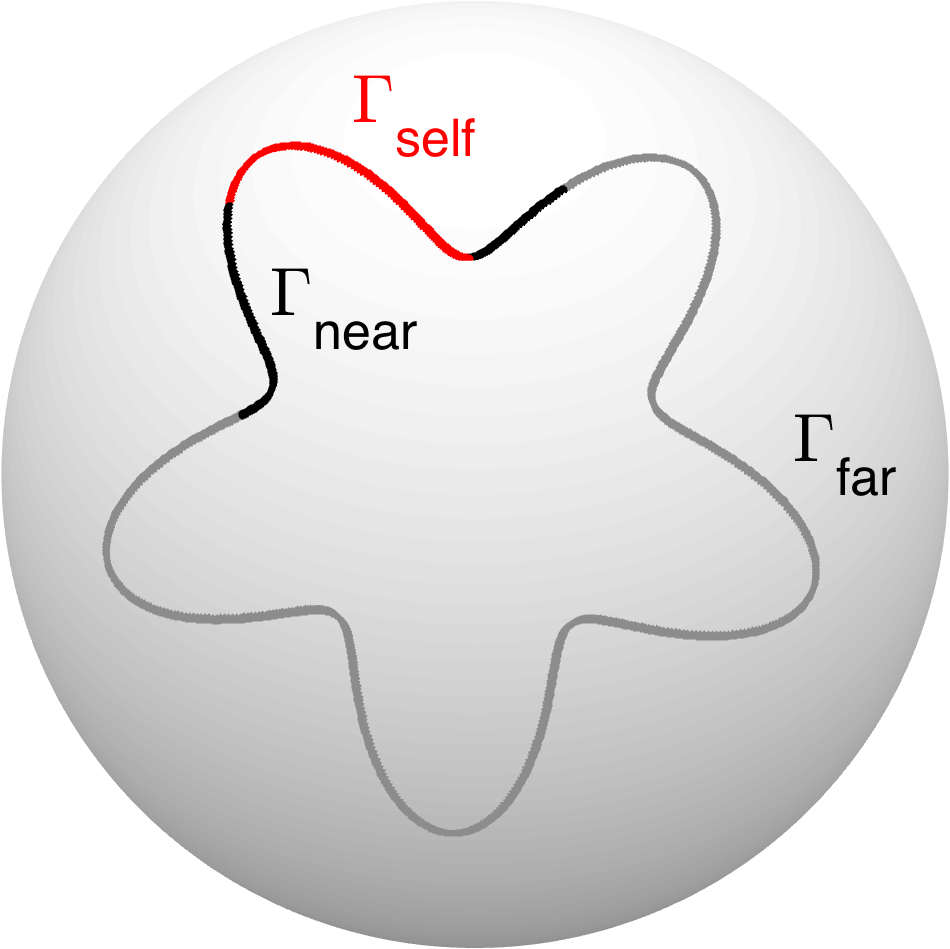
\includegraphics[width=0.3\textwidth]{SourcesSelfNearFar}
    	\caption{Sources on $\Gamma$ which contribute to the potential on $\Gamma_\tau$ (\ref{eq: PotentialGammaTau}) (also denoted by $\Gamma_{\text{self}}$).  $\Gamma_{\text{self}}$ represents sources due to self-interaction, while $\Gamma_{\text{near}}$ and $\Gamma_{\text{far}}$ represent the near and far field respectively.}
   	\label{fig: SourcesSelfNearFar}
\end{figure}

In terms of the matrix structure, the potential on each section of the contour $\Gamma_\tau$ corresponds to a row block of the matrix. Dividing the matrix $A=(I+K/ \pi)$ in (\ref{eq: LBSystem})
into four horizontal blocks for example, and splitting the sources based on the column indices corresponding to $\Gamma_{\text{self}}$, $\Gamma_{\text{near}}$ and $\Gamma_{\text{far}}$ we obtain \cite{CBMS}
\begin{align*}
	\begin{tabular}{ccccc}
	$A$ & $=$ & $\left(A^{(\text{self})} + A^{(\text{near})}\right)$ & $+$ & $A^{(\text{far})}.$\\
	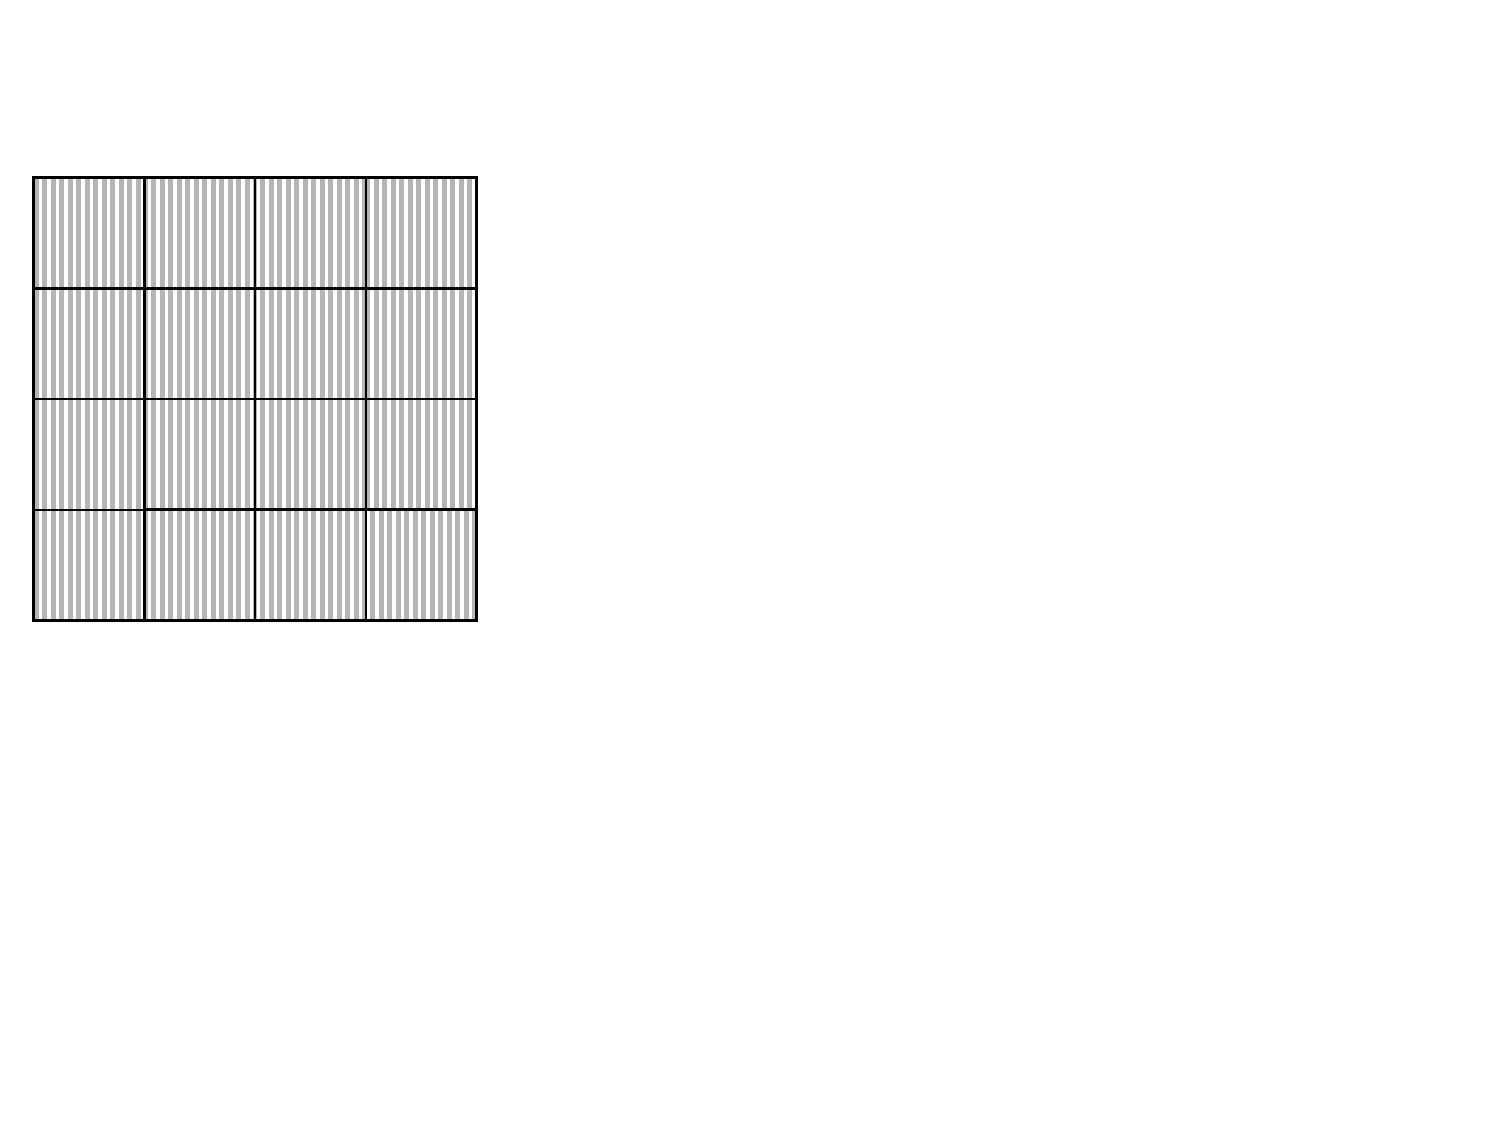
\includegraphics[width=3cm]{A_4by4}& & 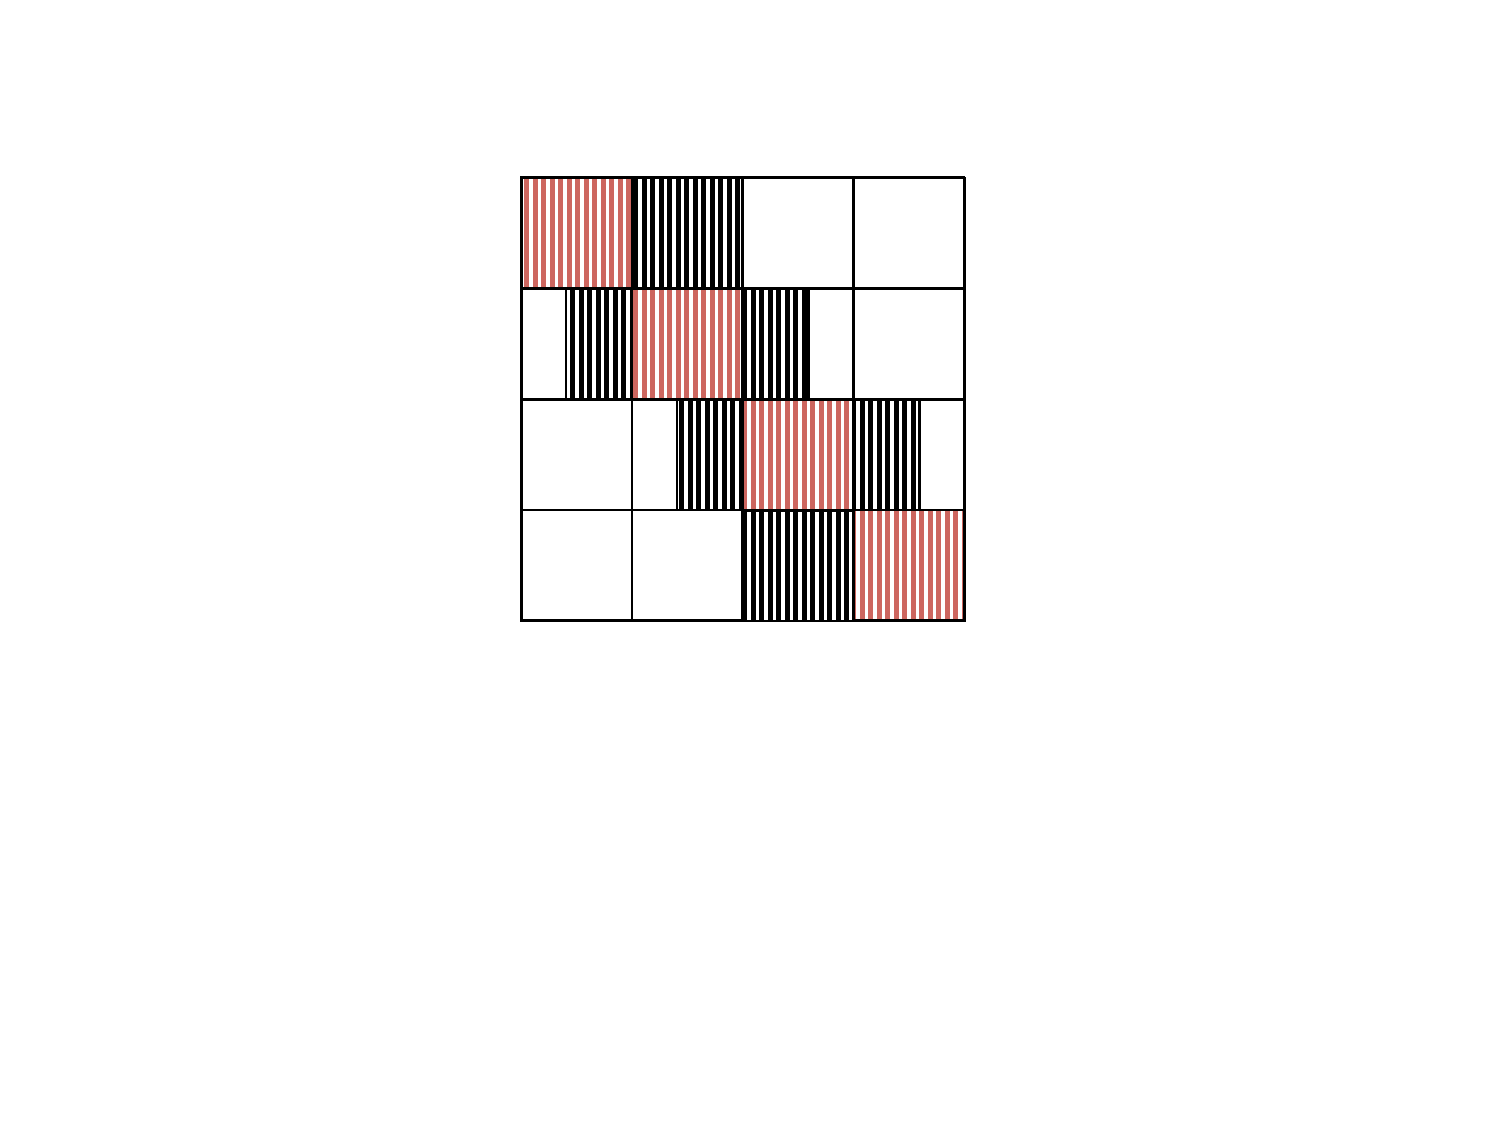
\includegraphics[width=3cm]{A_SelfNear} & & 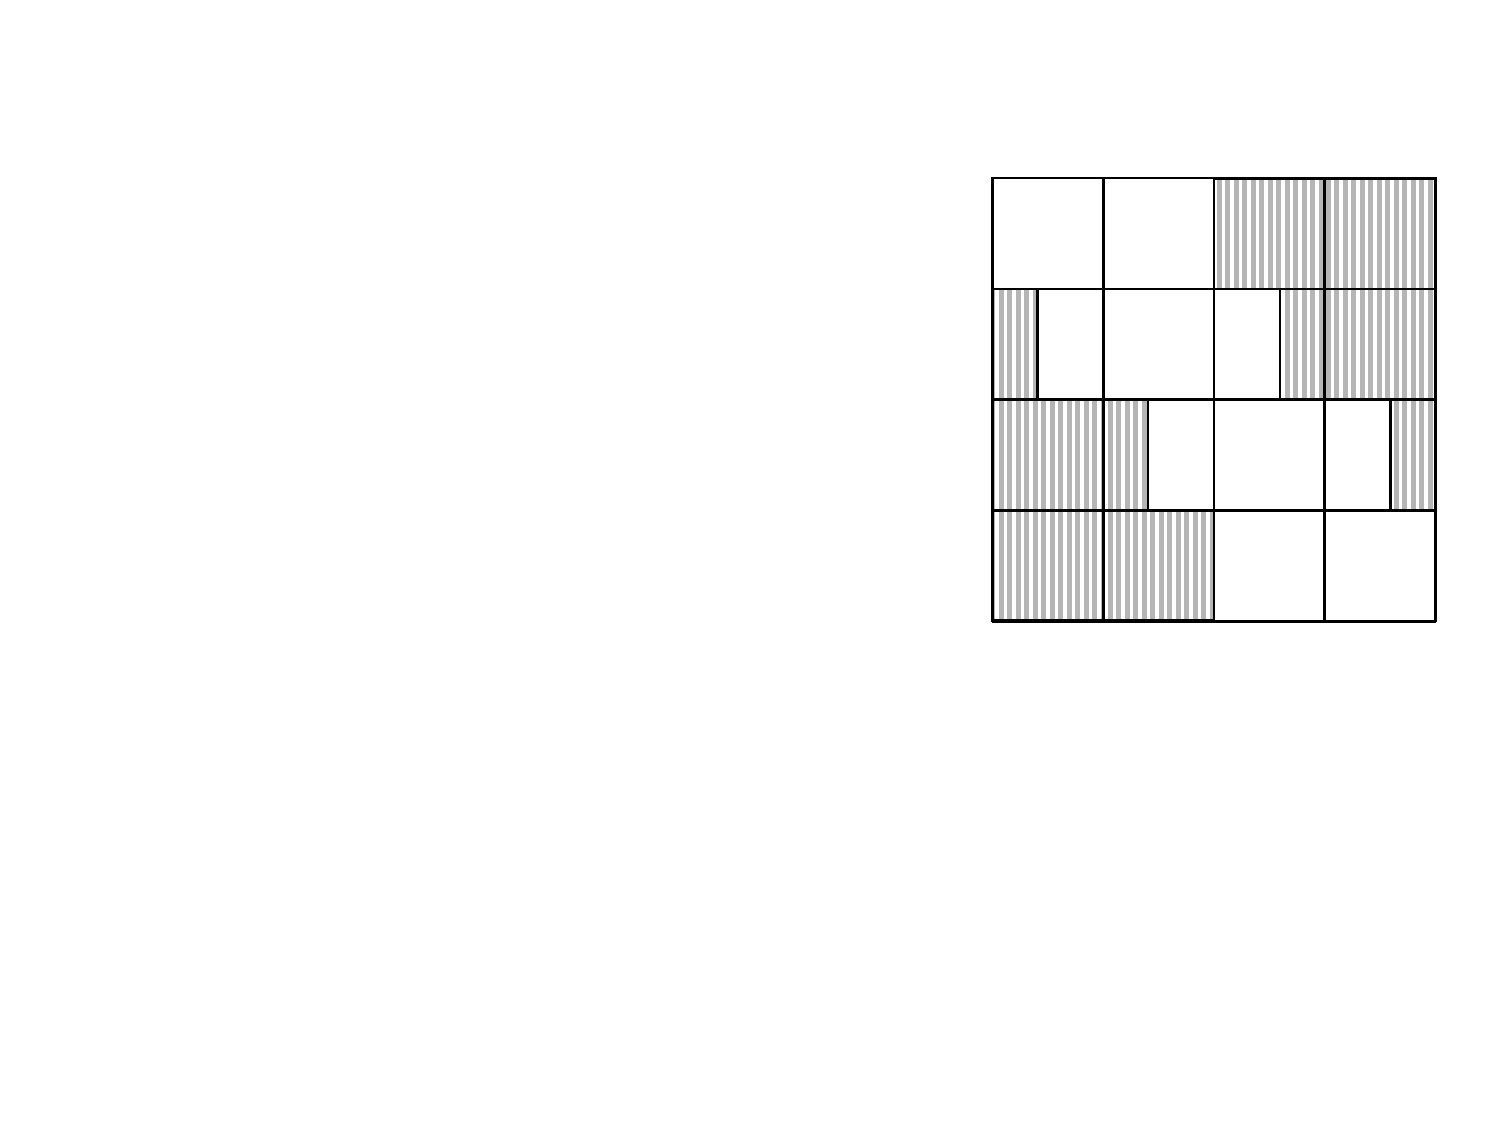
\includegraphics[width=3cm]{A_far}
	\end{tabular}
\end{align*}
The large contribution of the self interaction and near field terms gives $A$ a diagonally dominant structure. $A^{(\text{self})}$ is full rank, while $A^{(\text{near})}$ is close to full rank as well. The entries in $A^{(\text{far})}$ are rank-deficient due to the decay of the far field \cite{HoGreen2012, MartRokh2005}.  

Fast direct solvers group the near and far field blocks together, splitting the matrix into a diagonal and off-diagonal part,
\begin{align}
	\tabcolsep=0.05cm
	\begin{tabular}{ccccc}
	$A$ & $=$ & $A^{(\text{off})}$ & $ + $ & $D$.\\
	\raisebox{-0.45\height}{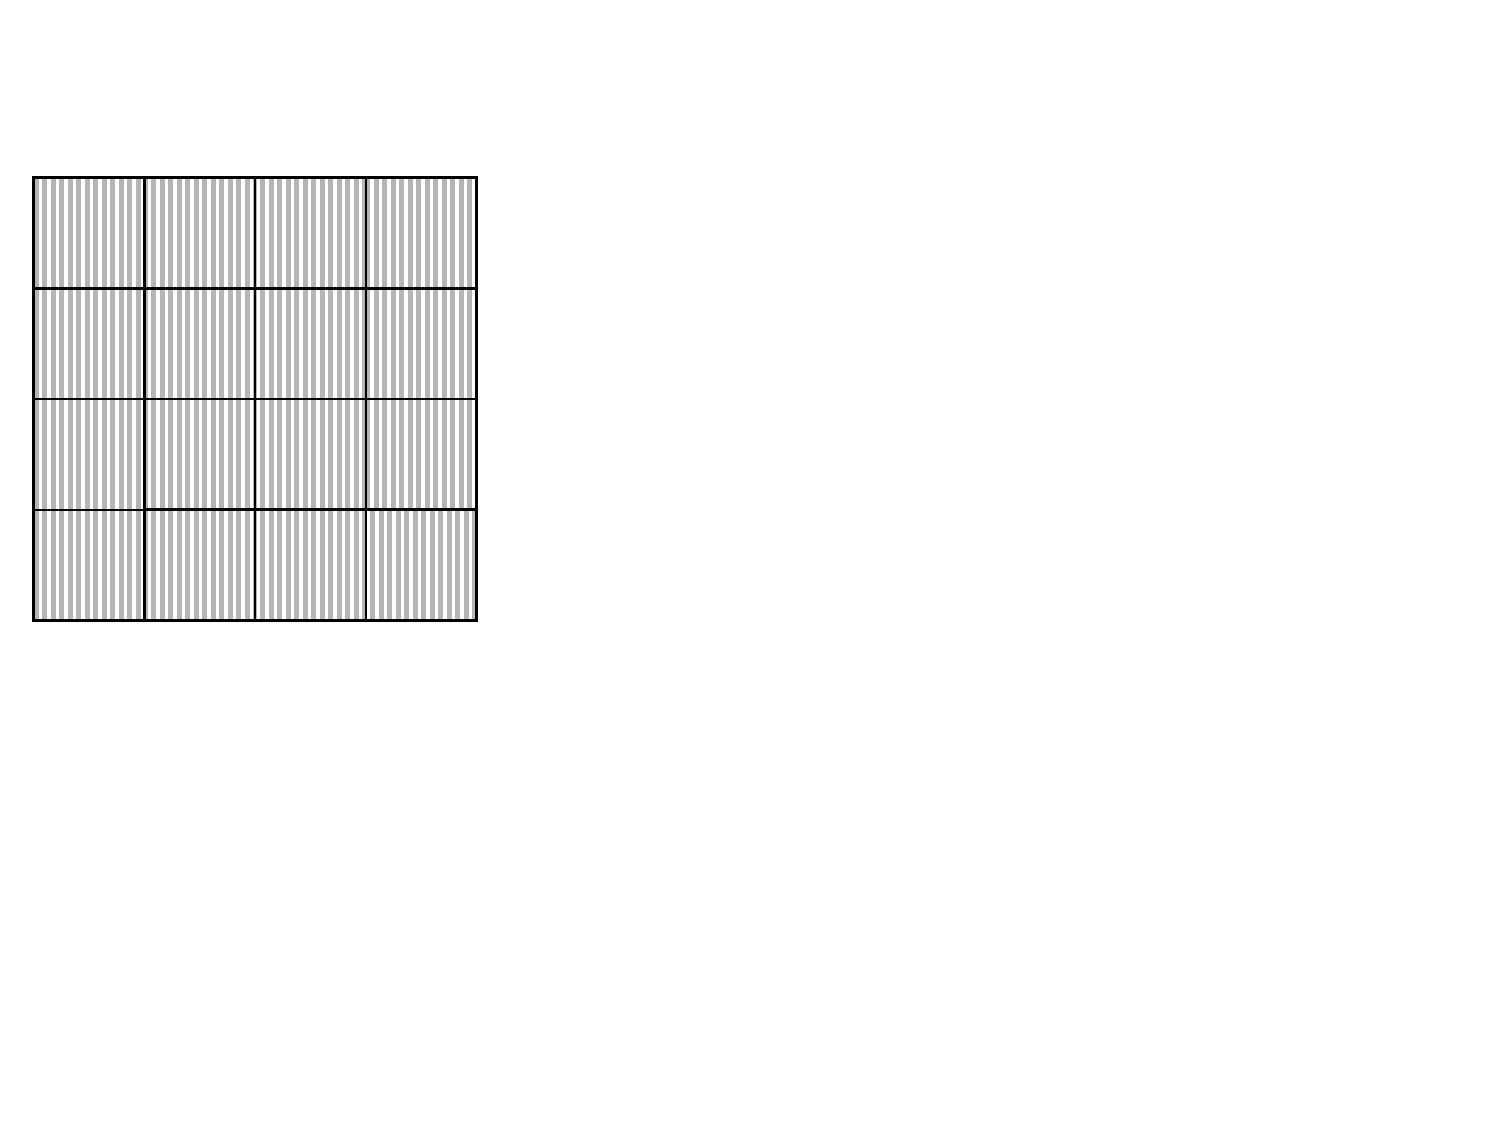
\includegraphics[width=3cm]{A_4by4}} & & $\left( \raisebox{-0.45\height}{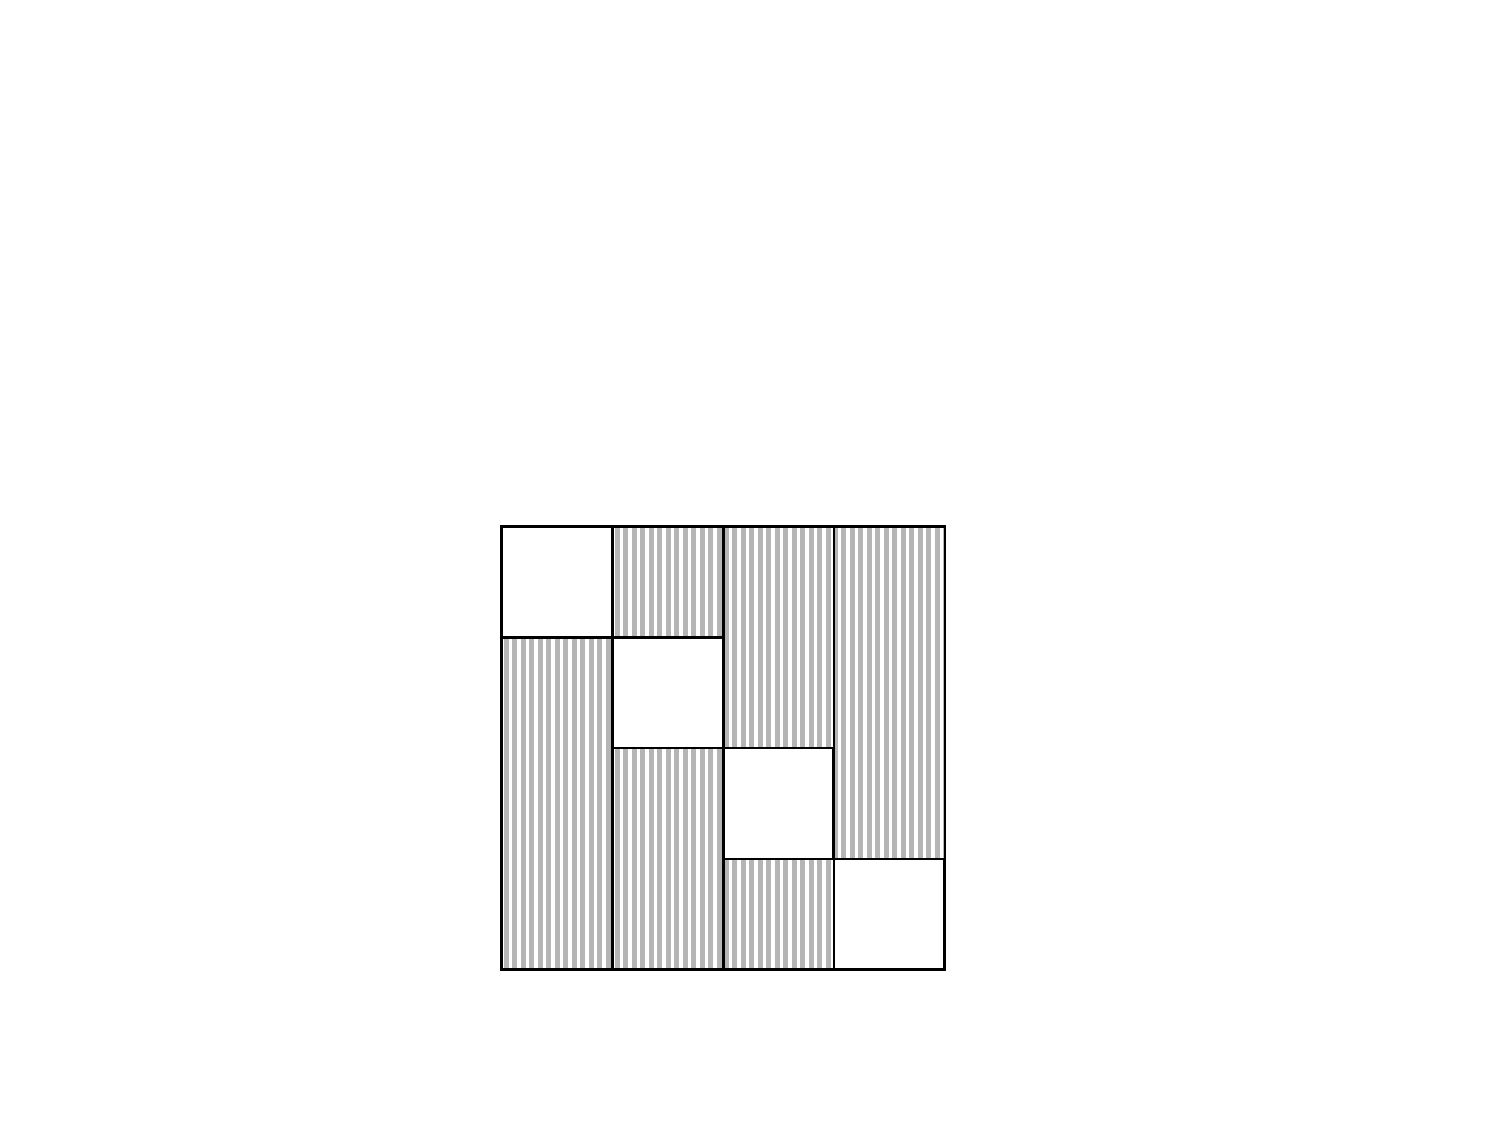
\includegraphics[width=3cm]{A_VerOffDiag}} = \raisebox{-0.45\height}{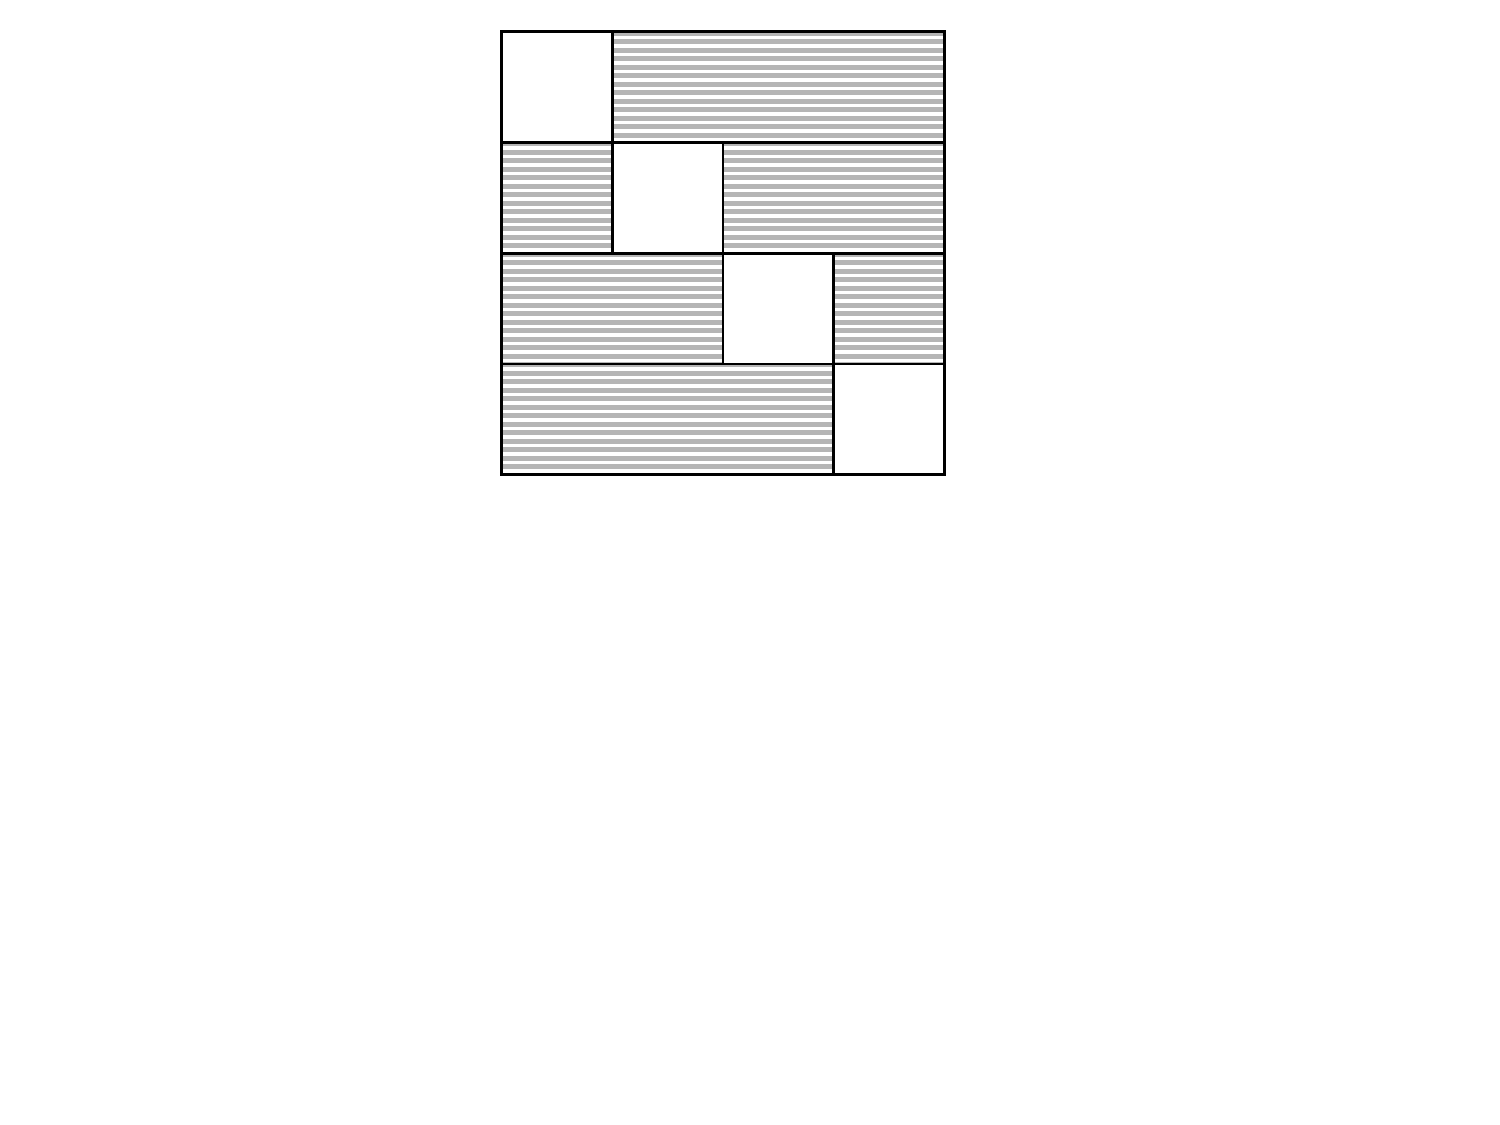
\includegraphics[width=3cm]{A_HorOffDiag}} \right)$ & & \raisebox{-0.45\height}{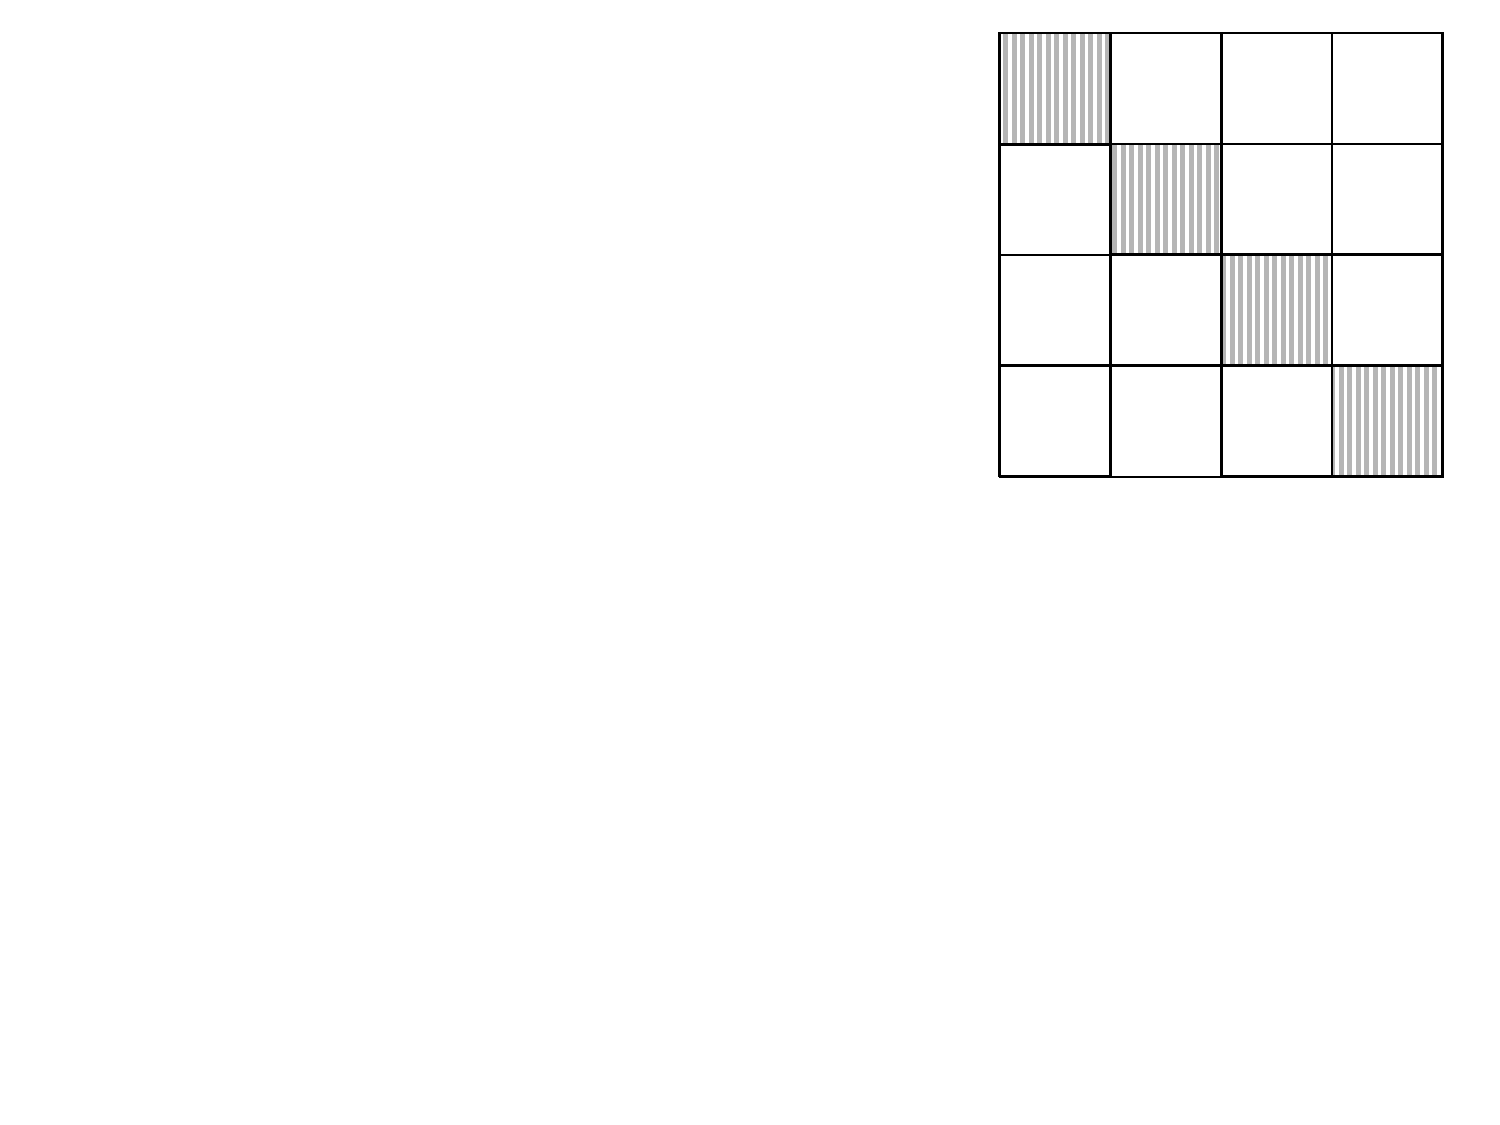
\includegraphics[width=3cm]{A_Diag}}
	\end{tabular}
	\label{eq: ADiagOffDiag}
\end{align}
The off-diagonal blocks can be grouped by row indices to form horizontal blocks, or by column indices to form vertical blocks. Row indices correspond to targets, where the potential is evaluated, while column indices correspond to sources. Both off-diagonal horizontal and vertical blocks are rank-deficient and have rapidly decaying singular values. An example of this decay for the horizontal off-diagonal blocks is shown in Figure \ref{fig: offdrank}. We note that the same decay can also be seen for the vertical blocks. 

\begin{figure}
	\centering
        \begin{subfigure}[b]{0.3\textwidth}
                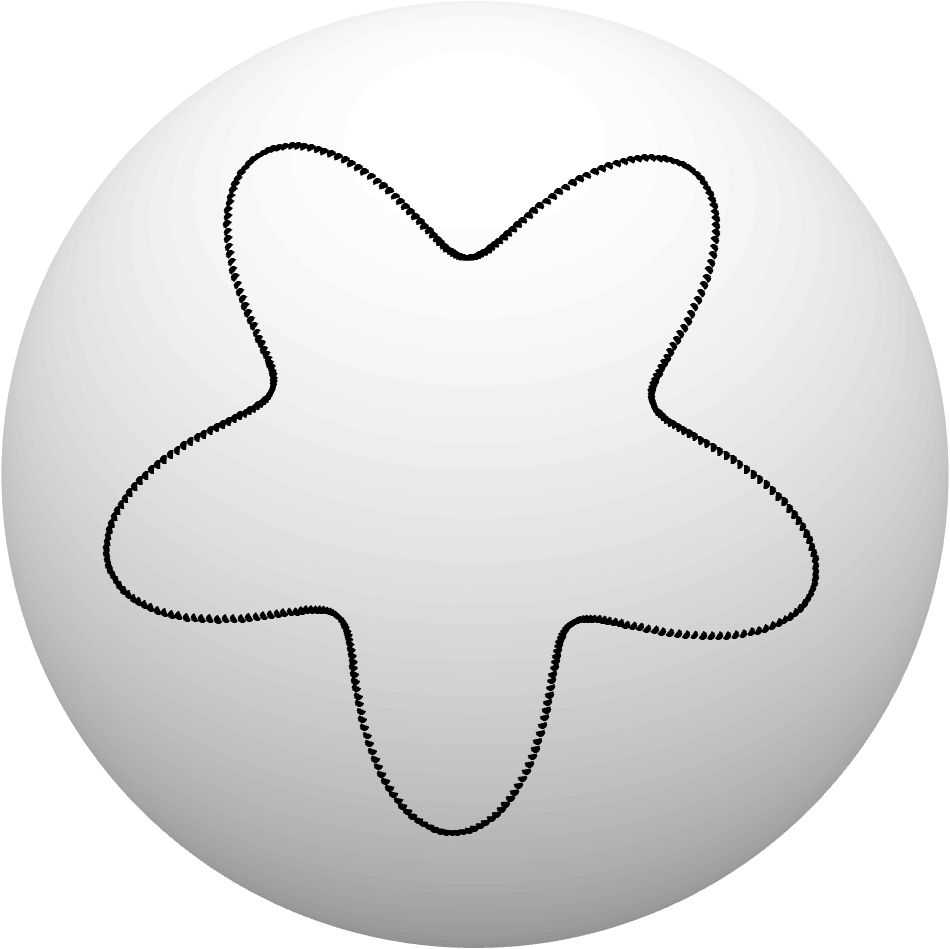
\includegraphics[width=\textwidth]{OffDiagExContour}
                \vspace{0.2cm}
                \caption{}
                \label{fig: OffDiagExContour}
         \end{subfigure}
        ~ 
        \hspace{1cm}
        \begin{subfigure}[b]{0.5\textwidth}
                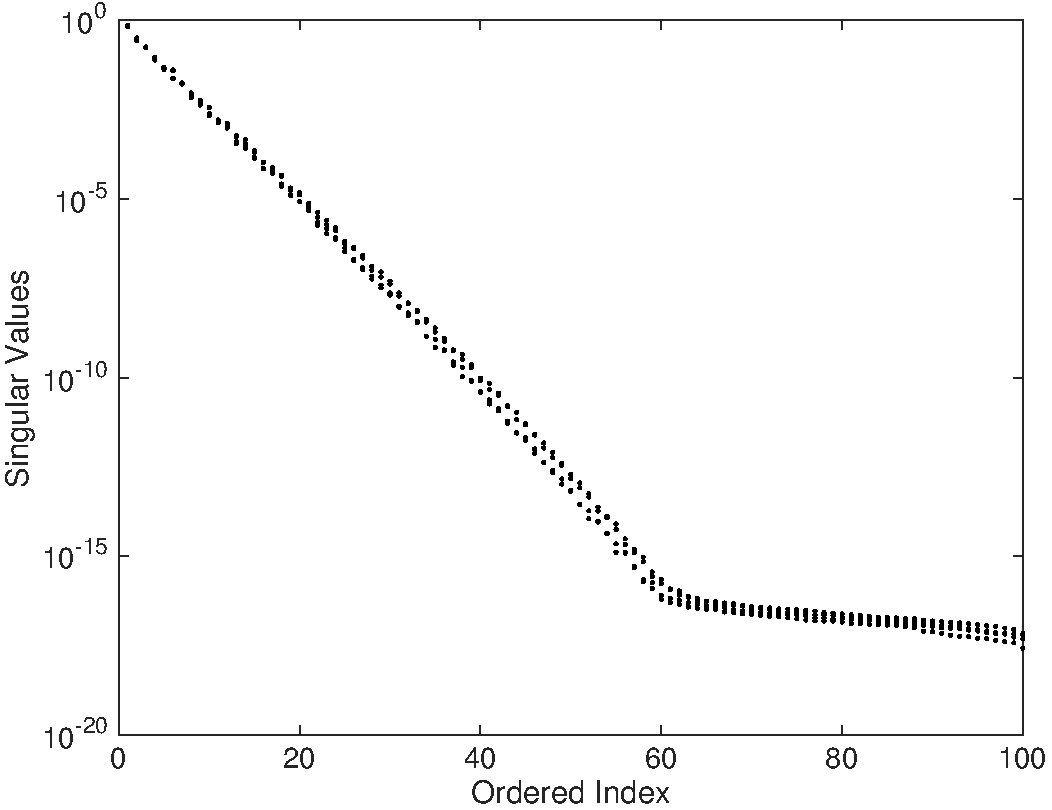
\includegraphics[width=\textwidth]{OffDiagSingValues}
                \caption{}
                 \label{OffDiagSingValues}
        \end{subfigure}
        \caption{(b) plots the singular values of the horizontal off-diagonal blocks corresponding to the matrix $(I+K/ \pi)$ in (\ref{eq: LBSystem}). For this example we take a star-shaped boundary (shown in (a)) and discretize the contour with $N=400$ points. The matrix is divided into $4 \times 4$ blocks as in (\ref{eq: ADiagOffDiag}). The dimension of each horizontal off-diagonal block is $100 \times 300$. The singular values of each block, plotted in (b), decay exponentially in this case. To machine precision each of the blocks has an approximate numerical rank of 60. }
        \label{fig: offdrank}
\end{figure}

% SECTION 3.2 --------------------------------------------------------------------------------------------------------------------------------------------------------------------------------------------
\section{The ID and Rank-Revealing QR}
\label{sec: ID}

Fast direct solvers exploit the rank-deficiency in BIE matrices by factoring the off-diagonal blocks of the system with the ID, which can be obtained by using rank-revealing QR. Given an $m\times n$ rank-deficient block $B$ and a tolerance $\varepsilon$, rank-revealing, or pivoted QR determines the approximate rank $k$ of the matrix and a basis for the column space \cite{Tref97, Bjorck96, Dax2000}. 

In the fast direct solver literature, Modified Gram Schmidt (MGS) is typically used to compute the pivoted QR \cite{ChengEtAl2005, GillYoungMart2012, MartRokh2005}. Given the matrix $B$, after $l=\min(m,n)$ steps, the algorithm will give a matrix $Q$ with orthonormal columns, and upper triangular matrix $R$ of the form
\begin{align*}
	B P=QR=\underset{m\times l}{\left[ \begin{array}{cc}
	Q_{11} & Q_{12}\\
	Q_{21} & Q_{22} \end{array} \right]}
	\underset{l \times n}{\left[ \begin{array}{cc}
	R_{11} & R_{12}\\
	0 & R_{22} \end{array} \right]}.
\end{align*}
Here, $P$ is an $n\times n$ permutation matrix, $Q_{11}$ is $k\times k$, $Q_{12}$ is $k\times (l-k)$, $Q_{21}$ is $(m-k) \times k$, and $Q_{22}$ is $(m-k)\times (l-k)$. $R_{11}$ is $k\times k$, $R_{12}$ is $k\times (n-k)$, and $R_{22}$ is $(l-k)\times (n-k)$. 
The columns of $B$ are pivoted in such a way that 
\begin{align*}
	Q_1=\left[ \begin{array}{c}
	Q_{11} \\
	Q_{21} \end{array} \right]
\end{align*} 
contains $k$ orthonormal vectors which span the range of the first $k$ linearly independent columns of $B P$. 
If $B$ has exact rank $k<l$ then $R_{22}$ is exactly zero \cite{Tref97, Bjorck96}. If we look at numerical rank, then $||R_{22}||<O(\varepsilon)$ \cite{Bjorck96, Dax2000, GuEis96}.
Hence one possible pivoting strategy \cite{Bjorck96, Dax2000} is to ensure the diagonal elements of $R$ are non-increasing, i.e.
\begin{align*}
	r_{11}\geq r_{22} \geq ... \geq r_{ll} \geq 0.
\end{align*}
Given a tolerance, $\varepsilon$, the algorithm terminates at step $k$, where ${||r_{kk}||}_2$ or ${||r_{kk}||}_F<O(\varepsilon)$. 

The cost of applying MGS with pivoting is $O(kmn)$ \cite{ChengEtAl2005, MartRokh2005}. It depends on the rank, $k$, of the block $B$, and its dimensions, $m$ and $n$. Applied as-is to the block $B$, this cost is also referred to as the brute force cost in the literature \cite{CBMS, CBMScode}. 

For the ID specifically, it is important to obtain as accurate a decomposition as possible. For this reason a double reorthogonalization step is also added. More details are provided in \cite{ChengEtAl2005, Bjorck94, Dax2000}. 

Using the pivoted QR algorithm, the matrix $B$ can be approximated by 
\begin{align*}
	B \approx \left[ \begin{array}{c}
				Q_{11} \\
				Q_{21} \end{array} \right]
	\left[ \begin{array}{cc}
				R_{11} & R_{12}\end{array} \right] P^*
\end{align*}
since $R_{22} \approx O(\varepsilon)$. 
Re-grouping the factors then gives the column ID for the matrix \cite{ChengEtAl2005},
\begin{align}
	B &\approx \underbracket{ Q_1 R_{11} }_{S_C}\underbracket{\left[ \begin{array}{cc}
												I_k & {R_{11}}^{-1} R_{12}\end{array} \right] P^*}_{V^*}, \nonumber \\
   	   &\approx \underset{ \ m\times k \ }{S_C} \underset{ \ k \times n \ }{V^*}, \label{eq: ColID}
\end{align}
where $S_C$ contains the $k$ linearly independent columns of $B$ which form a basis for the column space and $V^*$ holds the linear combinations of these columns. We also note that $V^*$ contains a $k\times k$ identity matrix corresponding to the $k$ columns chosen in $S_C$. 

If $B$ has exact rank $k$, then $\sigma_k>0$ and $\sigma_{k+1}= \sigma_{k+2}=...=\sigma_l=0$, where $l=\min(m,n)$, $\sigma_i$ denotes the $i^{th}$ singular value of $B$, and the singular values are arranged in non-increasing order,  $\sigma_1\geq \sigma_2 \geq ... \geq \sigma_l$. In this case,  the factorization (\ref{eq: ColID}) holds exactly \cite{GuEis96}.

Computationally, if $\sigma_{k+1}\approx O(\varepsilon)$ and $\sigma_k>>\sigma_{k+1}$, then $B$ is said to have numerical rank $k$ and (\ref{eq: ColID}) holds approximately with error bound \cite{GuEis96}
\begin{align}
	{||B-S_CV^*||}_2\leq \sigma_{k+1}(B)\sqrt{1+nk(n-k)}. \label{eq: IDError} 
\end{align}
The error depends on the ${(k+1)}^{\text{st}}$ singular value of $B$. If we write out the SVD of $B$ \cite{Tref97} we obtain
\begin{align}
	B&=\hat{U}\Sigma \hat{V}, \nonumber \\
         &=\sum_{i=1}^r \sigma_i \  \hat{u}_i \  \hat{v}_i^*. \label{eq: SVD}
\end{align}
where $r$ denotes the exact rank of the matrix, and $\hat{u}_i$ and $\hat{v}_i$ denote the columns of $\hat{U}$ and $\hat{V}$. 
Choosing a tolerance for the factorization (\ref{eq: ColID}) then truncates this sum at $i=k \leq r$. For example referring back to Figure \ref{fig: offdrank}, choosing a tolerance of $\varepsilon=10^{-10}$ will approximately retain the first $k=40$ terms in the sum (\ref{eq: SVD}), corresponding to the first 40 singular values of the off-diagonal blocks of the matrix A. 

Pivoted QR can also be applied to the rows of $B$ by factoring $B^*$: 
\begin{align*}
	B^*\tilde{P}\approx \tilde{Q}_1\left[\begin{array}{cc} \tilde{R}_{11} & \tilde{R}_{22} \end{array}\right].
\end{align*}
Re-grouping the factors then gives the row ID for $B$ \cite{ChengEtAl2005}
\begin{align*}
	\tilde{P}^*B& \approx {\left[ \begin{array}{cc} \tilde{R}_{11} & \tilde{R}_{22} \end{array}\right]}^* \tilde{Q}_1^*,\\
	&\approx \tilde{P}\left[\begin{array}{c}\tilde{R}_{11}^* \\ \tilde{R}_{22}^*\end{array}\right] \tilde{Q}_1^*,\\
	& \approx \underbracket{\tilde{P} \left[\begin{array}{c} I_k \\ \tilde{R^*_{12}}{(\tilde{R^*}_{11})}^{-1} \end{array} \right]}_{U} \underbracket{ \left[ \begin{array}{cc} \tilde{R^*}_{11}\tilde{Q_1^*} \end{array} \right]}_{S_R},\\
	& \approx \underset{ \ m \times k \ }{U}\underset{ \ k \times n \ }{S_R}.
\end{align*}
Here, $S_R$ contains the $k$ linearly independent rows of $B$ which form a basis for the row space, and $U$ contains the linear combinations of $S_R$ which form $B$. 

We can also combine the two factorizations together by first applying the column ID to $B$, 
\begin{align*}
	B \approx \underset{\ m\times k \ }{S_C}\underset{k \times n}{V^*},
\end{align*}
and then applying the row ID to $S_C$,
\begin{align*}
	S_C \approx \underset{\ m \times k \ }{U}\underset{ \ k \times k \ }{S}.
\end{align*}
This gives the full ID for $B$,
\begin{align*}
	B=\underset{ \ m \times k \ }{U} \underset{\ k\times k \ }{S}\underset{ \ k \times n \ }{V^*}.
\end{align*}
The matrix $S$ is a $k \times k$ submatrix of $B$, which is comprised of $k$ linearly independent rows and columns, while $U$ and $V^*$ both contain $k \times k$ identity matrices and have norms close to 1 \cite{ChengEtAl2005}. The ID represents each row of $B$ as a linear combination of $k$ selected rows, and each column of $B$ as a linear combination of $k$ selected columns. As a result the matrix $S$ is referred to as the compressed representation of $B$, or its "skeleton" matrix. We can think of the "action" of $B$ as being represented through the action of its submatrix $S$ \cite{ChengEtAl2005}. Since obtaining the ID for the matrix $B$ requires pivoted QR to be applied twice, the cost of the ID is also $O(kmn)$. 

The advantage of this factorization is that $S$ is represented by the intersection of $k$ rows and columns of $B$, which we will see allows for a more straightforward physical interpretation of the ID, especially once it is applied recursively in Section \ref{sec: BFRecCompression}. Since the matrices $U$ and $V^*$ both contain identity matrices, they can be constructed more efficiently than in other matrix factorizations such as the SVD \cite{Tref97}. 

% SECTION 3.3 -------------------------------------------------------------------------------------------------------------------------------------------------------------------------------------------
\section{Single Level Brute Force Compression}
\label{sec: SingLevel}
To apply the ID to the matrix $A$ in (\ref{eq: LBSystem}) arising from the discretization of the Laplace-Beltrami BIE (\ref{eq: LB_BIE}), the matrix is first divided into $p$ blocks of size $n$. 

To clearly show how the single level algorithm works, we first work through a specific example with $p=4$, and $N=400$ as in (\ref{eq: ADiagOffDiag}) and Figure \ref{fig: offdrank}.  Let $I_\tau$, and $L_\tau=\{1, ..., pn\} \backslash I_\tau$, $\tau=1,...,4$ denote the index vectors for the rows and columns of the $\tau^{th}$ off-diagonal row block. Then the ID can be applied one by one to each off-diagonal block. 

If we look at the first horizontal off-diagonal block, $A(I_1, L_1)$, and apply the row ID, we obtain 
\begin{align*}
	\begin{tabular}{ccc}
	$\underset{ n \times 3n }{A(I_1, L_1)}$ &$\approx$ & $\underset{ \ n \times k \ }{U_1}\underset{ \ k \times 3n \ }{S_{R_1}.}$\\
	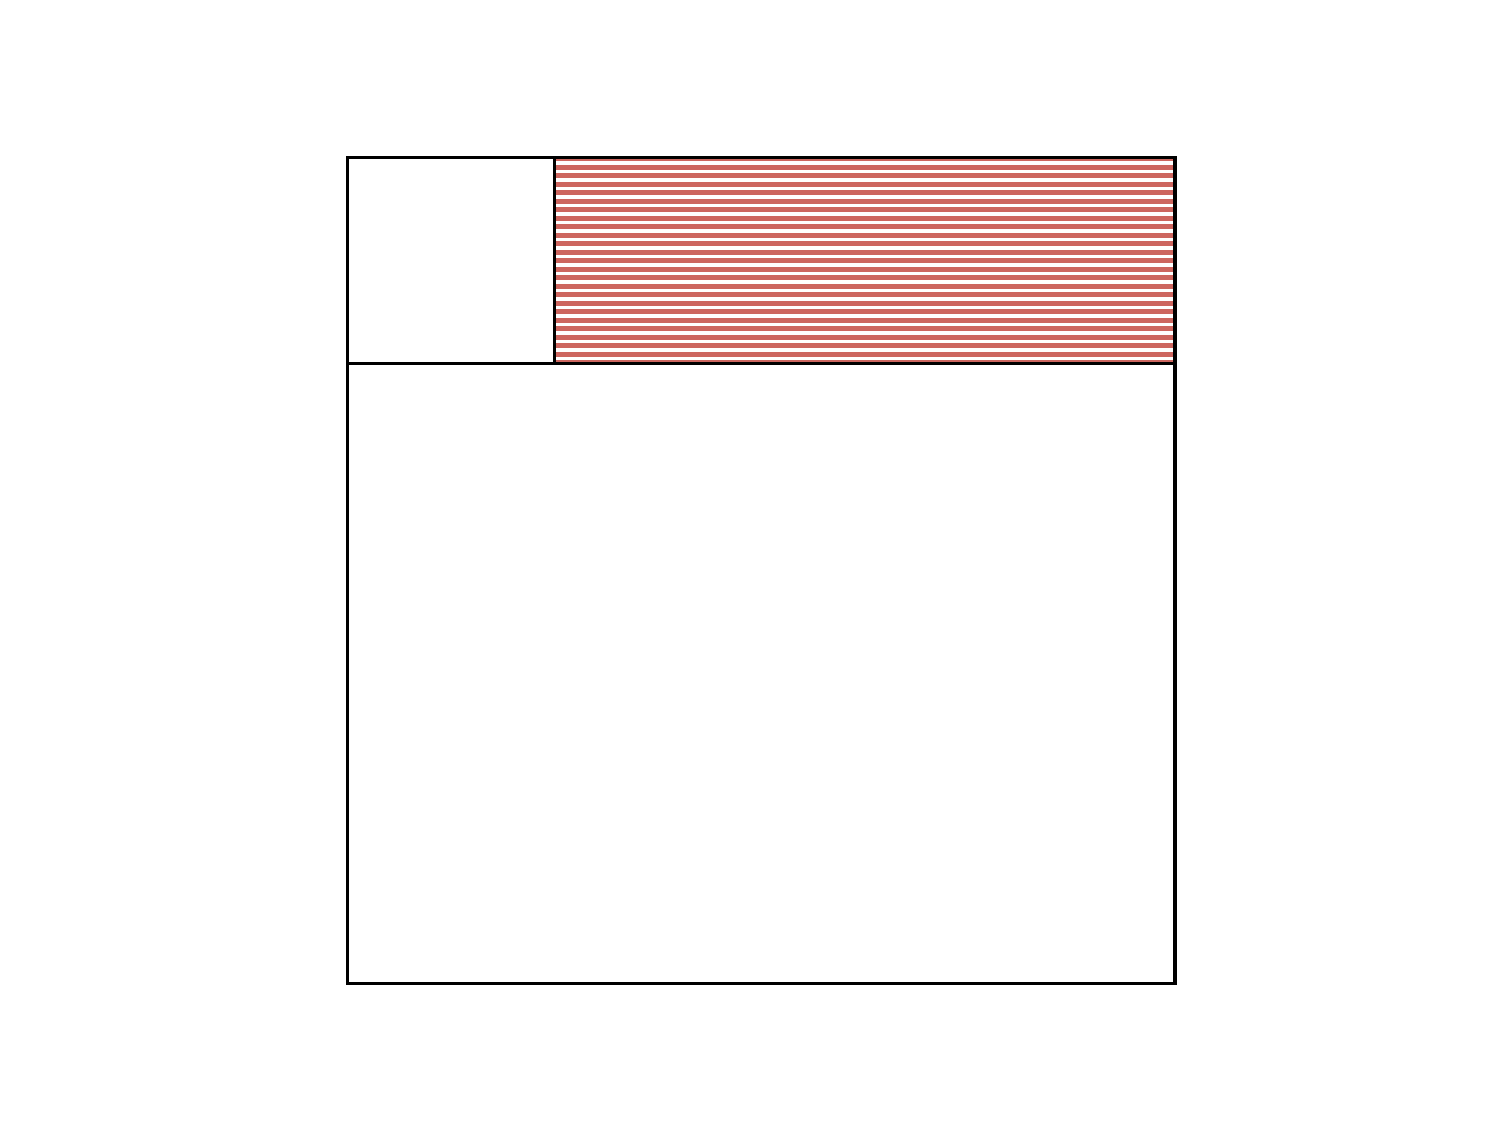
\includegraphics[width=0.3\textwidth]{SingLevelHorBlock1} & & 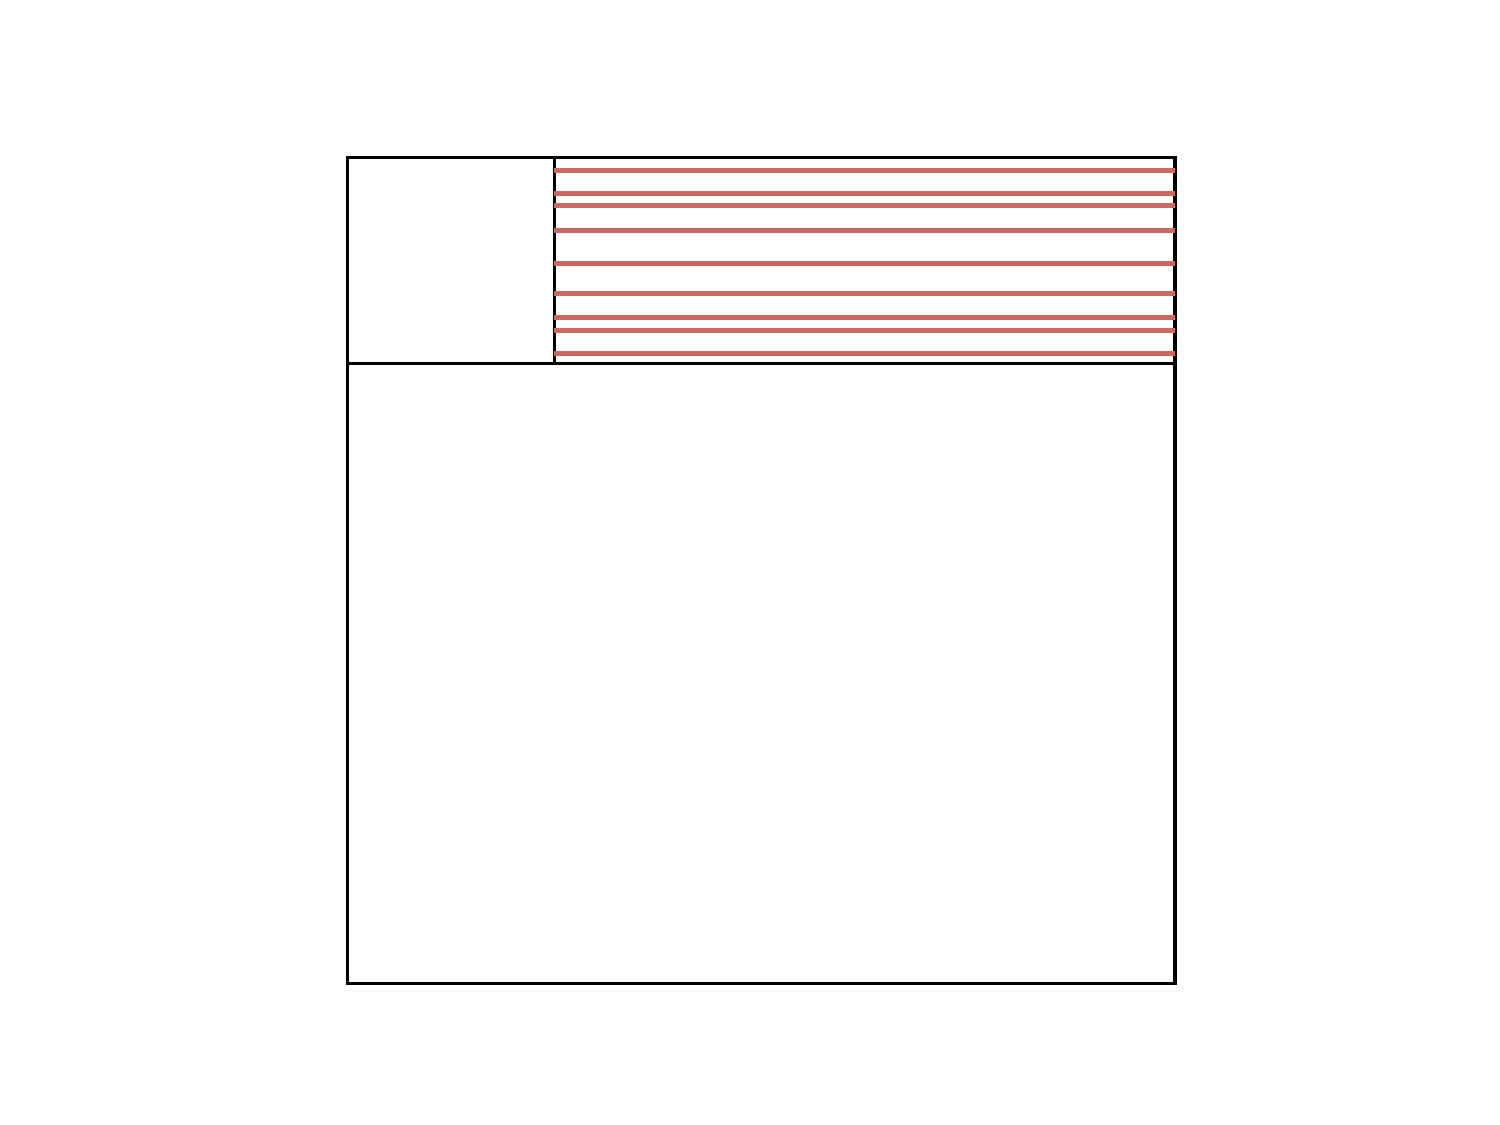
\includegraphics[width=0.3\textwidth]{SingLevelHorSkel1}
	\end{tabular}
\end{align*}

Here, the colour red is used to denote the row indices, $I_1$, of the block. $S_{R_1}$ contains the $k$ rows of $A(I_1, L_1)$  selected by the ID, shown in the matrix on the right. The factorization can equivalently be interpreted as representing each column of $A(I_1, L_1)$ as a linear combination of the columns of $U_1$. This implies that the columns of $U_1$ form a basis for the columns of the horizontal off-diagonal block. 

Likewise, the same procedure can be applied to the second row block, $A(I_2, L_2)$, which gives 
\begin{align*}
	\begin{tabular}{ccc}
	$\underset{ n \times 3n }{A(I_2,L_2)}$ & $\approx$ & $\underset{ \ n \times k \ }{U_2} \underset{ \ k \times 3n \ }{S_{R_2}.}$ \\
	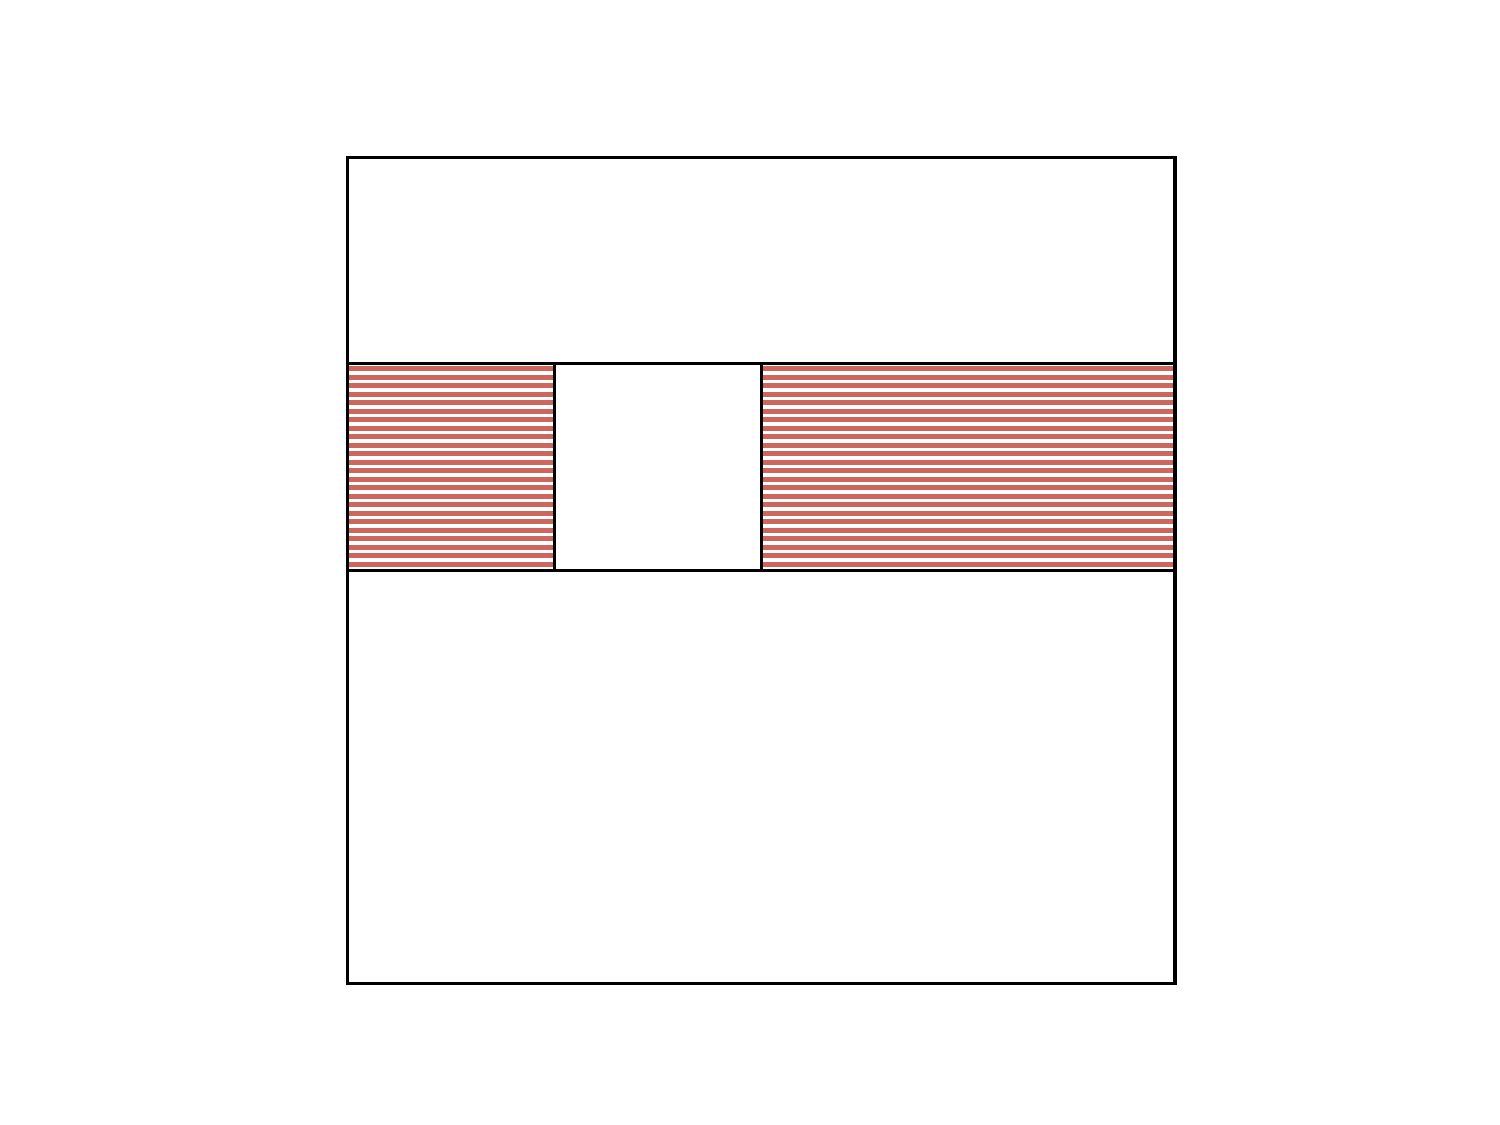
\includegraphics[width=0.3\textwidth]{SingLevelHorBlock2}& & 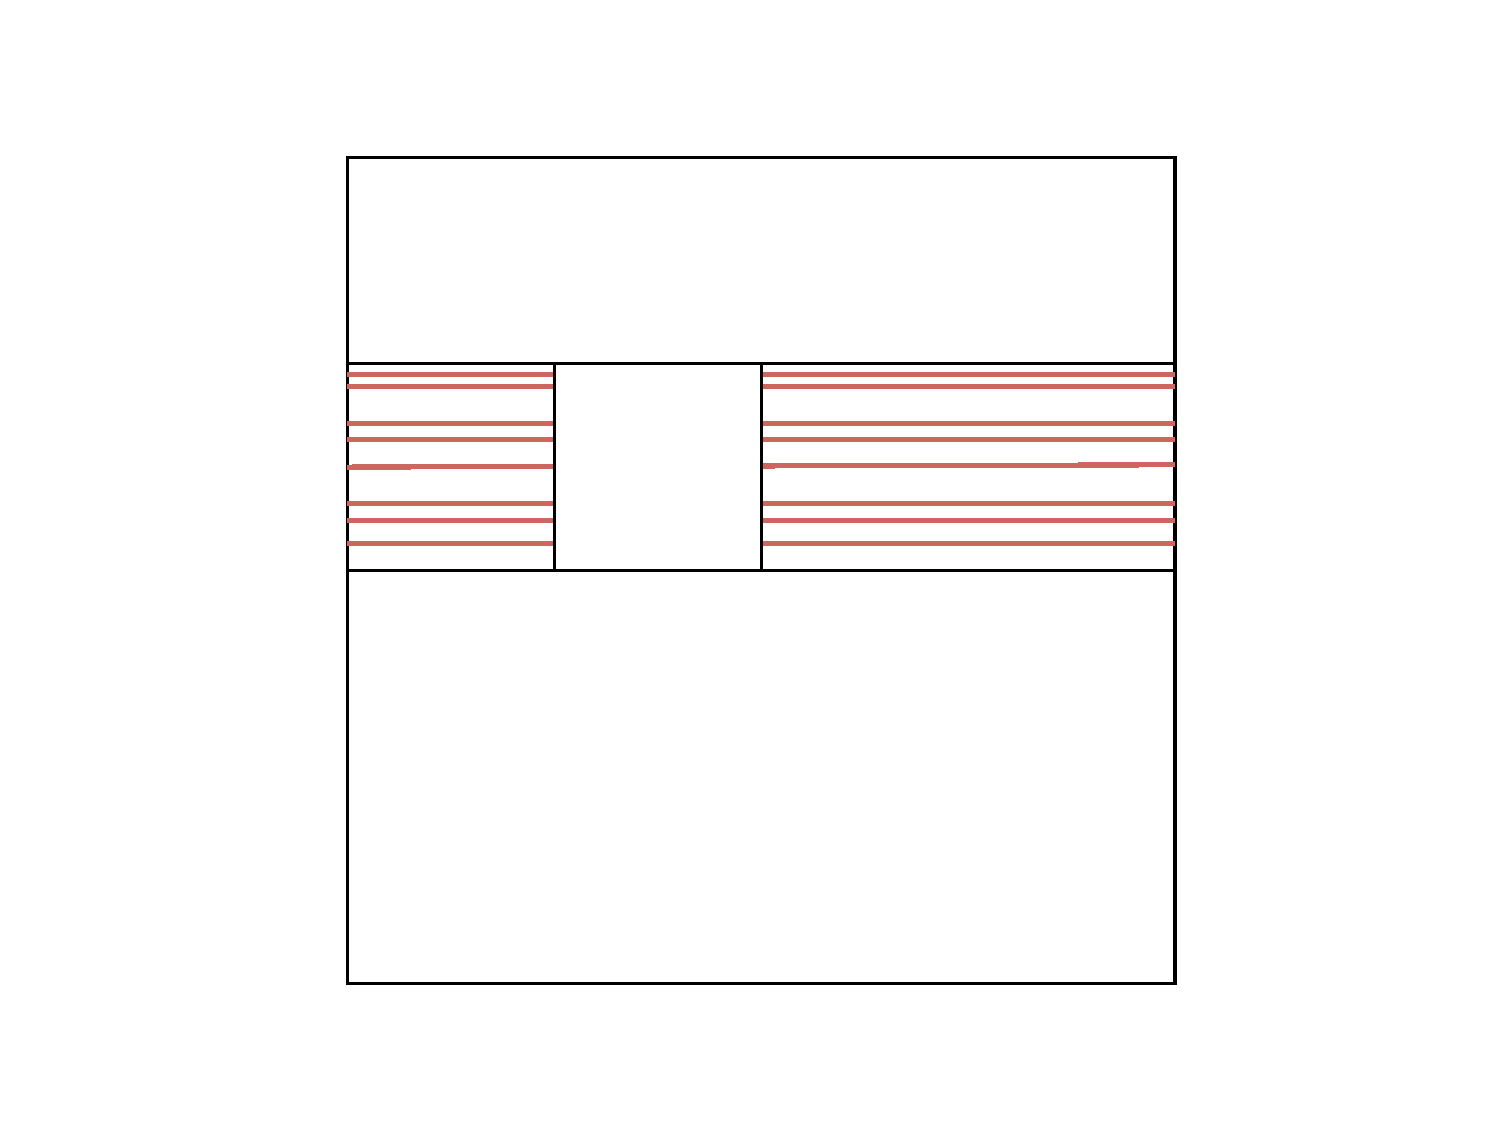
\includegraphics[width=0.3\textwidth]{SingLevelHorSkel2}
	\end{tabular}
\end{align*}

For simplicity we assume that all horizontal and vertical blocks have the same numerical rank $k$, although this is not required by the compression algorithm. The ID determines the rank of each block based on the level of precision assigned. 

Continuing through the matrix, we can obtain factorizations for $A(I_3, L_3)$ and $A(I_4, L_4)$. 

The vertical blocks are then compressed in the same way. Applying the ID to the first vertical block gives
\begin{align}
\begin{tabular}{ccc}
	$\underset{ 3n \times n }{A(L_1, I_1)}$ & $\approx$ & $\underset{ \ 3n \times k \ }{S_{C_1}}\underset{ \ k \times n \ }{V_1^*,}$ \\
	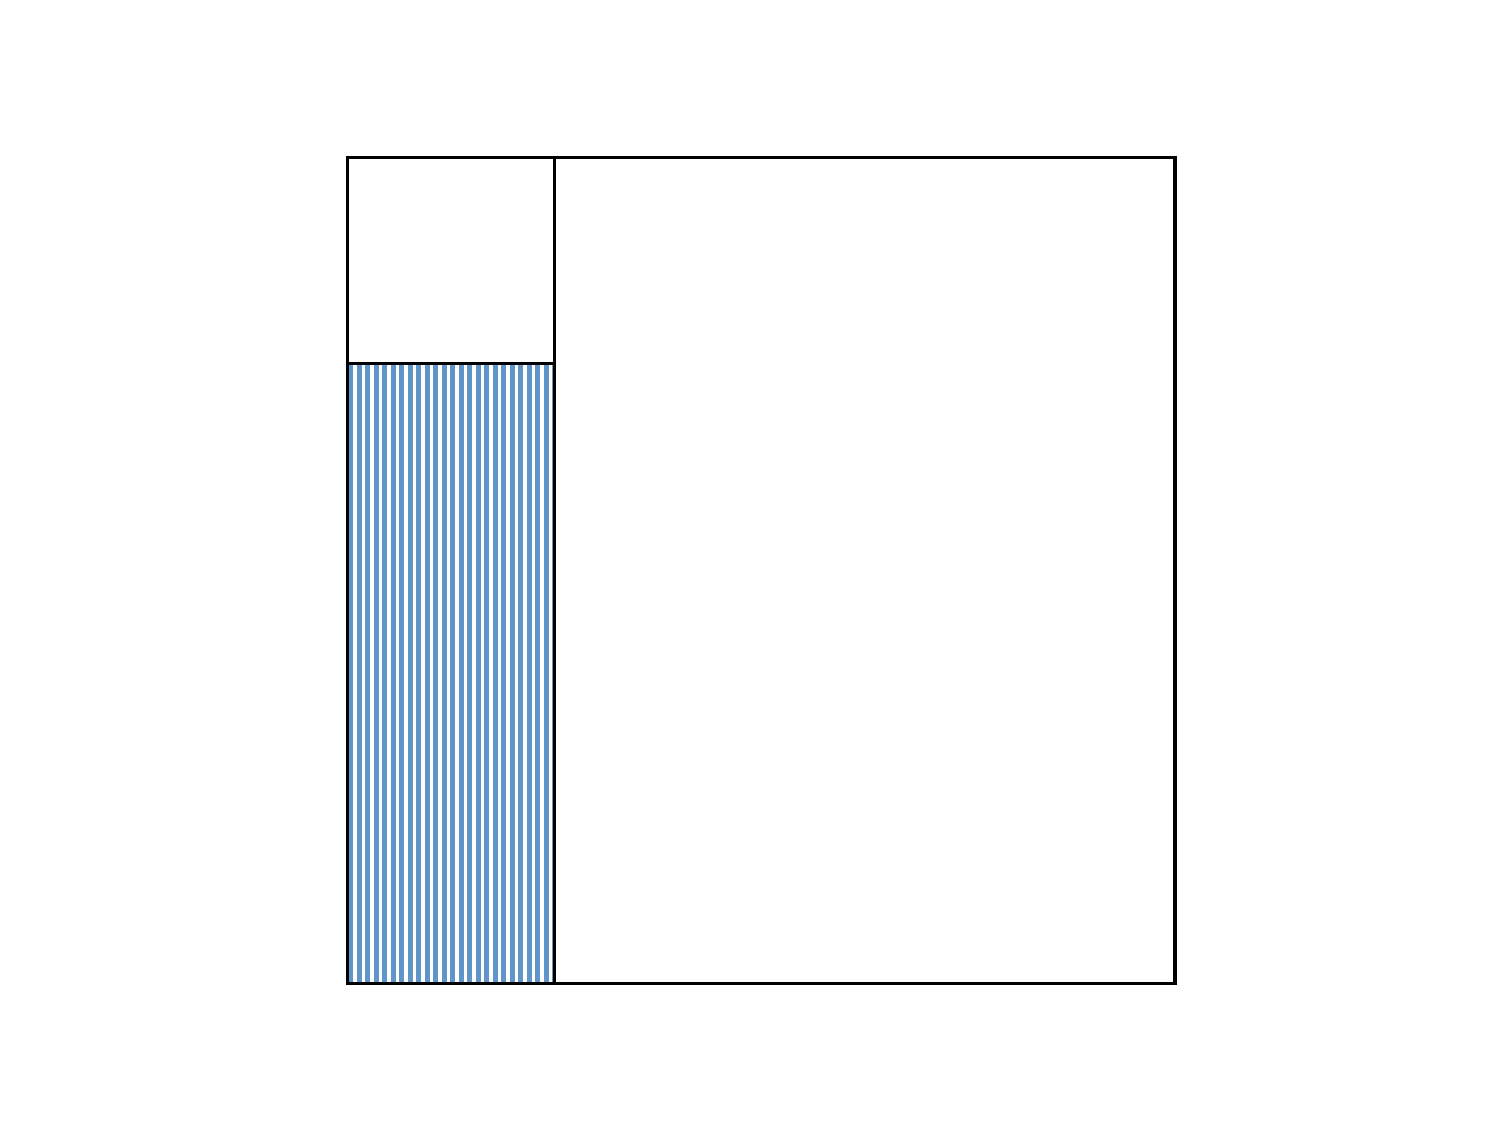
\includegraphics[width=0.3\textwidth]{SingLevelVertBlock1} & & 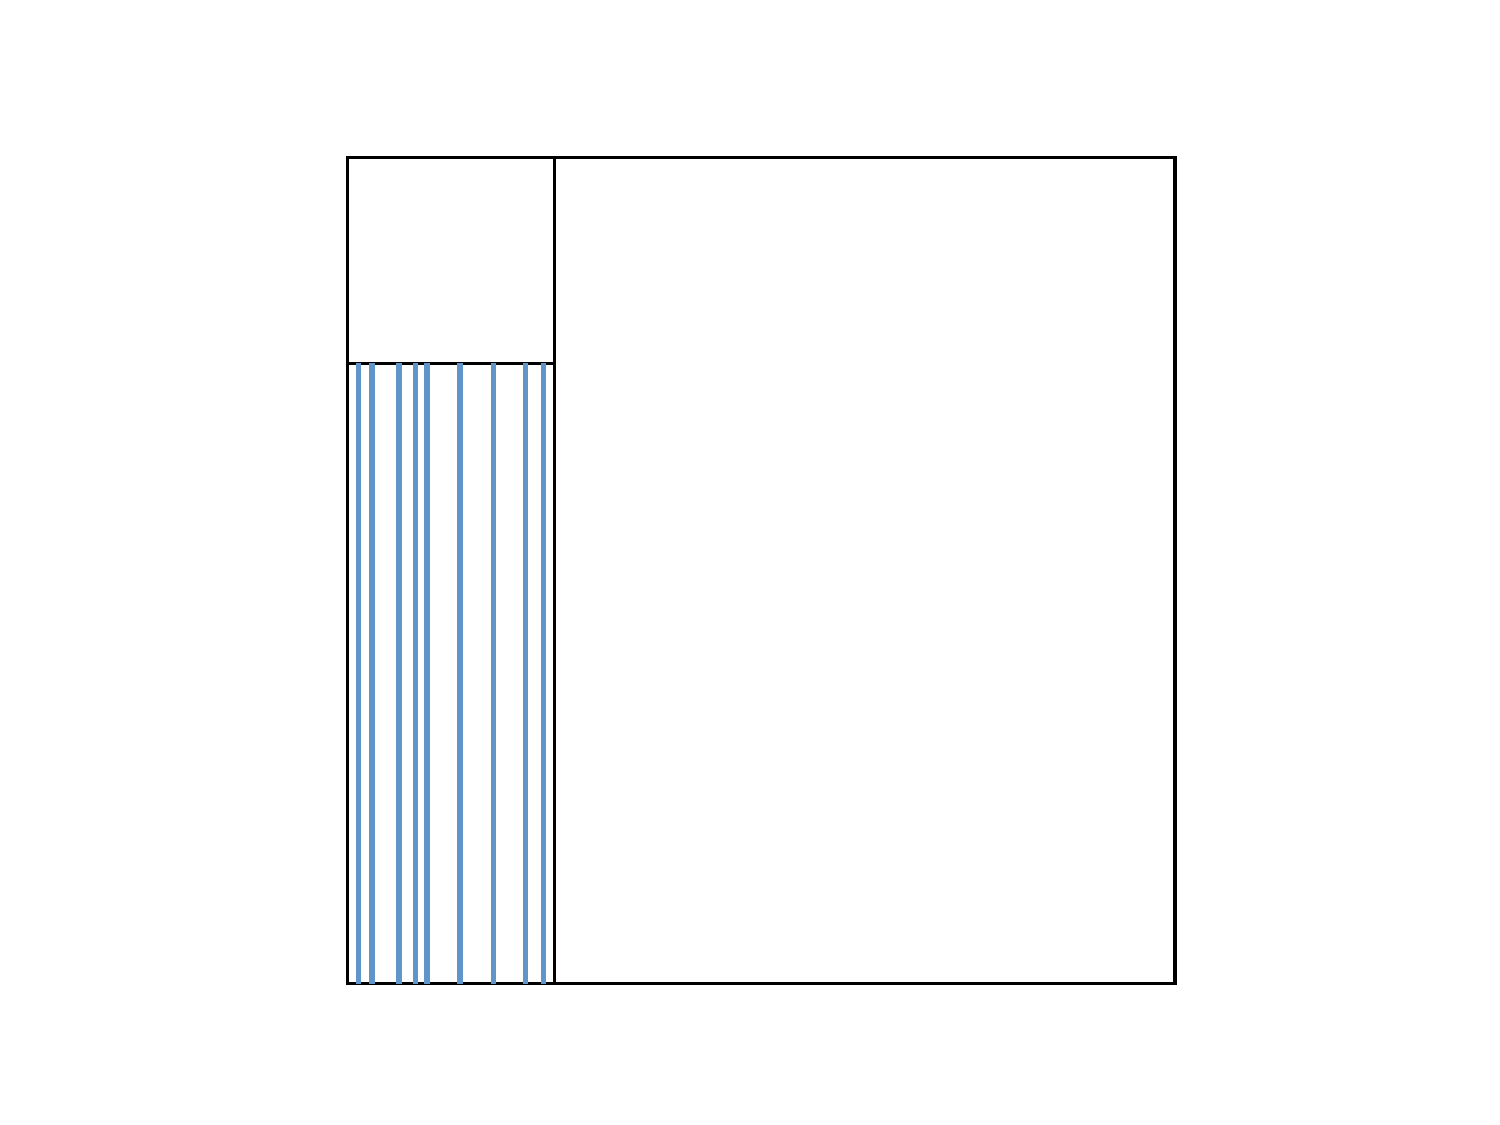
\includegraphics[width=0.3\textwidth]{SingLevelVertSkel1}
	\end{tabular}
	\label{eq: SingLevelVerBlock}
\end{align}
where we use blue to denote the column indices of the vertical block. $S_{C_1}$ contains the $k$ columns of $A(L_1, I_1)$ selected by the ID, which are shown on the right. Also, taking the transpose of (\ref{eq: SingLevelVerBlock}), we have 
\begin{align*}
	A^*(L_1, I_1) \approx V_1S_{C_1}^*.
\end{align*}
Just as with the row ID, this implies that (\ref{eq: SingLevelVerBlock}) can be equivalently interpreted as representing each row of the vertical block as a linear combination of the columns of $V_1$. 

After applying this procedure to all vertical blocks, we have 
\begin{align*}
	A\approx \left[\begin{array}{cccc}
	A_{11} & U_1S_{12}V_2^* & U_1S_{13}V_3^* & U_1S_{14}V_4^*\\
	U_2 S_{21}V_1^* & A_{22} & U_2 S_{23} V_3^* & U_2 S_{24} V_4^*\\
	U_3 S_{31}V_1^* &U_3 S_{32} V_2^* & A_{33} & U_3 S_{34} V_4^*\\
	U_4 S_{41} V_1^* & U_4 S_{42} V_2^* & U_4 S_{43} V_3^* & A_{44}
\end{array}\right].
\end{align*}
Note that each matrix $U_i$ is a basis for the columns in the $i^{th}$ off-diagonal row block, and each matrix $V_j$ is a basis for the rows in the $j^{th}$ off-diagonal column block. 

At this point $A$ can be separated into its diagonal and off-diagonal components, which gives 
\begin{align*}
	A&\approx \hspace{3.4cm}A^{(\text{off})} \hspace{3.6cm} + \hspace{1.9cm}D.\hspace{3cm}\\
         &\approx \left[\begin{array}{cccc}
	0 & U_1S_{12}V_2^* & U_1S_{13}V_3^* & U_1S_{14}V_4^*\\
	U_2 S_{21}V_1^* & 0 & U_2 S_{23} V_3^* & U_2 S_{24} V_4^*\\
	U_3 S_{31}V_1^* &U_3 S_{32} V_2^* & 0 & U_3 S_{34} V_4^*\\
	U_4 S_{41} V_1^* & U_4 S_{42} V_2^* & U_4 S_{43} V_3^* & 0
\end{array}\right] +  \left[\begin{array}{cccc}
	A_{11} & & & \\
 	& A_{22} &  & \\
 	& & A_{33} & \\
 	& &  & A_{44}
\end{array}\right]
\end{align*}
The matrices $U_i$ and $V_j$ can then be factored to give 
\begin{align}
	A &\approx \left[ \begin{array}{cccc}
                         U_1& & & \\
                               & U_2 & & \\
                               &         &U_3&\\
                               &         &          &U_4 
                               \end{array} \right] \left[\begin{array}{cccc}
                                                                  0&S_{12}& S_{13} &S_{14}\\
                                                                  S_{21}&0 & S_{23} &S_{24}\\
                                                                  S_{31}& S_{32} & 0& S_{34} \\
                                                                  S_{41}& S_{42} &S_{43}& 0
                                                                  \end{array}\right]
                                                             \left[\begin{array}{cccc}
                                                             V^*_1& & & \\
                               			         & V^*_2 & & \\
                               				&         &V^*_3&\\
                               				&         &          &V^*_4
                               				\end{array} \right]  \ +  \ \ \ D \nonumber \\
										&\approx \underset{4n \times 4k} { \hspace{1.5cm} U \hspace{1.5cm}  }\underset{4k \times 4k}{ \hspace{2.1cm} S  \hspace{2.1cm}  } \underset{4k \times 4n}{ \hspace{1.8cm} V^* \hspace{1.6cm} }+ \  \underset{4n \times 4n}{ D.} \label{eq: SingLevelFactorization} 
\end{align}
We can see that the above factorization for $A$ is comprised of block diagonal factors, and a smaller, dense skeleton matrix, $S$.

\subsubsection{Cost of Single Level Brute Force Compression and Inversion}
The cost of obtaining the factorization (\ref{eq: SingLevelFactorization}) is determined by summing up the cost of the ID for each off-diagonal block, which is determined from the cost of pivoted QR. For general $p$ and $n$, the cost of applying the ID to one horizontal and vertical off-diagonal block is $O(2kn(p-1)n)$. Since there are $p$ diagonal blocks, this procedure is applied $p$ times, giving a total approximate cost of $O(kp^2n^2) = O(kN^2)$. Thus compressing $A$ depends on the cost of the ID/QR which depends on the ranks and dimensions of the off-diagonal blocks. 

A matrix which can be decomposed into the compressed factorization (\ref{eq: SingLevelFactorization}) is called \textit{block-separable} \cite{GillYoungMart2012, HoGreen2012}. Due to the special form of this factorization, existing formulas for matrix inversion can be applied. Specifically, a variation of the following classical Sherman-Morrison-Woodbury formula can be used \cite{GillYoungMart2012}. \\

\noindent \textbf{Sherman- Morrison-Woodbury Formula}\\
Suppose $A$ is an invertible matrix in the form given in (\ref{eq: SingLevelFactorization}), and that the matrices, $D$, $V^*D^{-1}U$, and $S + {(V^*D^{-1}U)}^{-1}$ are also invertible. 
Then the inverse of $A$ is given by 
\begin{align*}
	A^{-1}=E{(S+\hat{D})}^{-1}F^* + G, 
\end{align*}
where 
\begin{align*}
	\hat{D} &= {(V^*D^{-1}U)}^{-1},\\
	E &= D^{-1}U\hat{D}, \\
	F &=  {(\hat{D}V^*D^{-1})}^*, \\
	G &= {D}^{-1} - D^{-1}U\hat{D}V^*D^{-1}. 
\end{align*}

Since $U$, $V$, and $D$ are block diagonal, $\hat{D}$, $E$, $F$ and $G$ can be evaluated rapidly. The cost of then inverting $A$ can be shown to drop from $O(p^3n^3)$ to $O(pn^3+p^3k^3)$ \cite{GillYoungMart2012}. The details are omitted since we use a different inversion strategy which will be discussed in Section \ref{sec: umfpack}. The Sherman-Morrison-Woodbury formula is mentioned here, since our inversion strategy follows similar principles and has similar costs. 

The total cost then for compression, inversion and solution of the system is $O(kp^2n^2+pn^3+p^3k^3)$, which has a small computational gain over $O(N^3)$ \cite{GillYoungMart2012}. 
To really see a difference, we need to apply  this single level scheme recursively. 

% SECTION 3.4 -------------------------------------------------------------------------------------------------------------------------------------------------------------------------------------------
\section{Recursive Brute Force Compression}
\label{sec: BFRecCompression}
The key observation that fast direct solvers make is that $S$ in (\ref{eq: SingLevelFactorization}) is also block separable. If $S$ is split into larger blocks, then rank deficiencies can be reintroduced into the off-diagonal blocks which can be recompressed by the same scheme as above. 

We illustrate this recursive process by applying it to a specific example, similar to Section \ref{sec: SingLevel}. This is also based on examples shown by Gillman et al. in \cite{GillYoungMart2012} and Martinsson, in \cite{CBMS} for the planar case. 
To obtain an efficient recursive algorithm, we take the total number of points, $N$, which for this example we set to $N=400$, and place the index vector $I=[1, ..., N]$ on a binary tree. The number of points, $n_l$ on each level, $l$, is successively halved, until we reach a desired number of points, $n_1$, on the finest level, $l=1$. In this case $n_1=50$. The resulting binary tree is given by, 
\begin{align}
	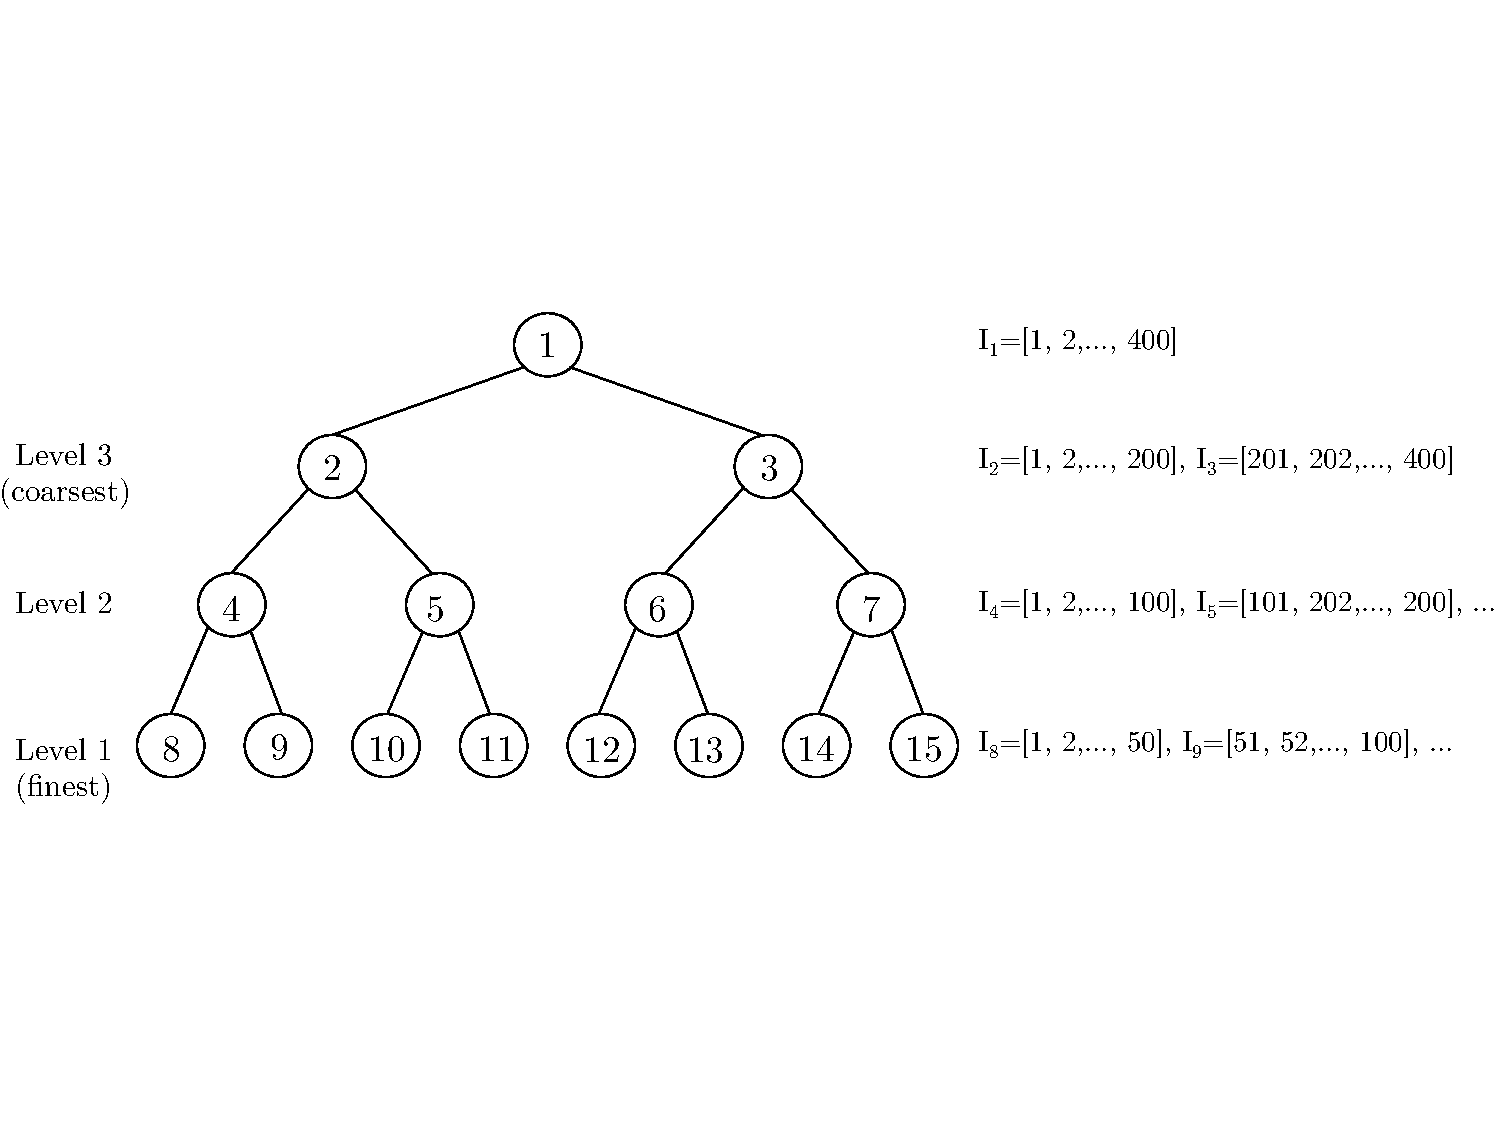
\includegraphics[width=\textwidth]{BinaryTree} \label{eq: BinaryTree} 
\end{align}

The finest level on the bottom of the tree is labelled as level $l=1$ since this is where the recursive algorithm begins. The number of leaves on this level represents the initial number of blocks, $p_1$, in the matrix. At each successive level the number of blocks, $p_1$, is halved until we reach the coarsest level, $l=\lambda$, where $p_\lambda=2$. In (\ref{eq: BinaryTree}), $\lambda=3$.

The binary tree corresponds to successively halving the boundary contour into smaller and smaller sections (Figure \ref{fig: ContourBinaryTree}). In this example, we take the same star-shaped boundary as in Figure \ref{fig: OffDiagExContour}. 

\begin{figure}
        \centering
        \begin{subfigure}[b]{0.23\textwidth}
         \captionsetup{justification=centering}
                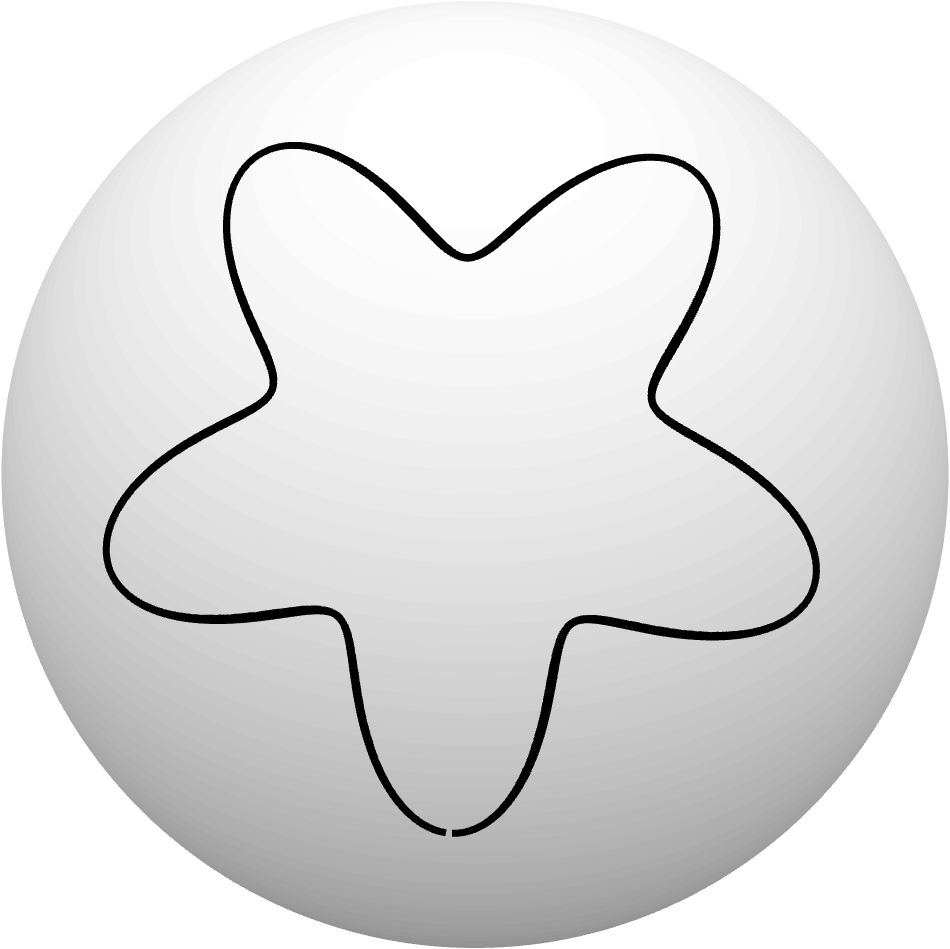
\includegraphics[width=\textwidth]{ContourRoot}
                \caption{Root of tree: \\$\Gamma=\Gamma_1$}
               \label{fig: ContourRoot}
        \end{subfigure}%
        ~ 
         \begin{subfigure}[b]{0.23\textwidth}
         \captionsetup{justification=centering}
                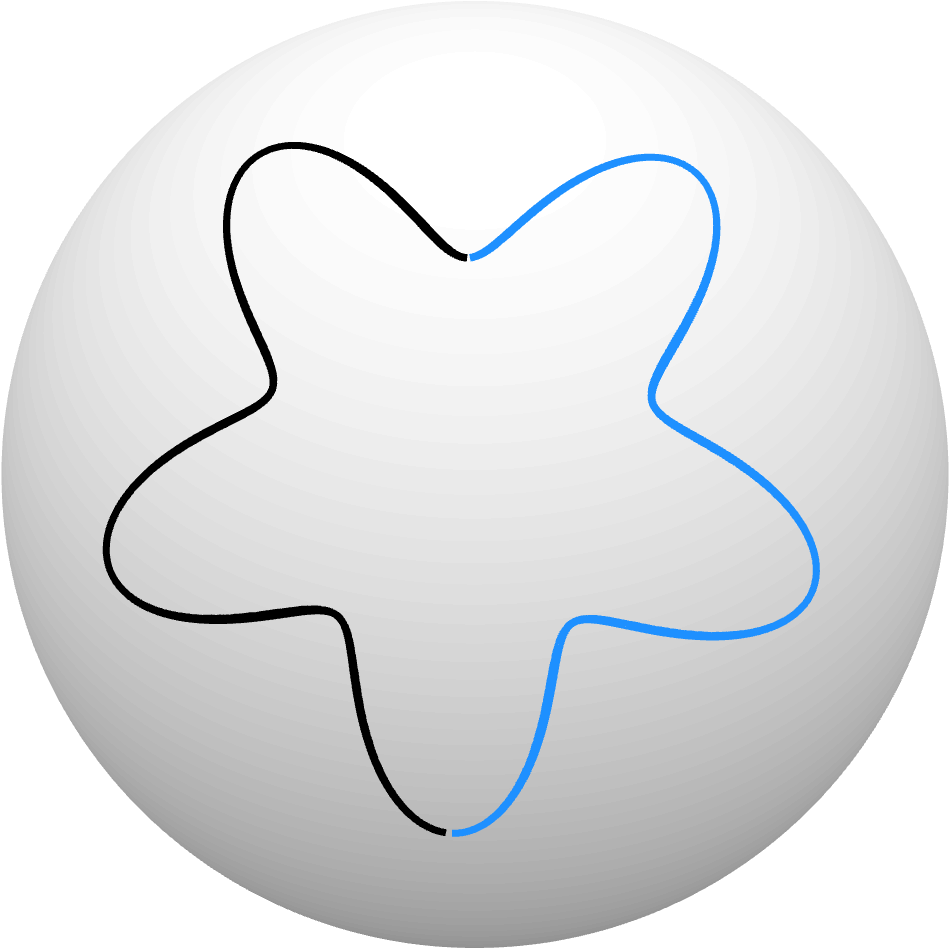
\includegraphics[width=\textwidth]{ContourLevel3}
                \caption{Level 3: \\$\Gamma_2 \cup \Gamma_3$}
                \label{fig: ContourLevel3}
        \end{subfigure}
        ~ 
        \begin{subfigure}[b]{0.23\textwidth}
        \captionsetup{justification=centering}
                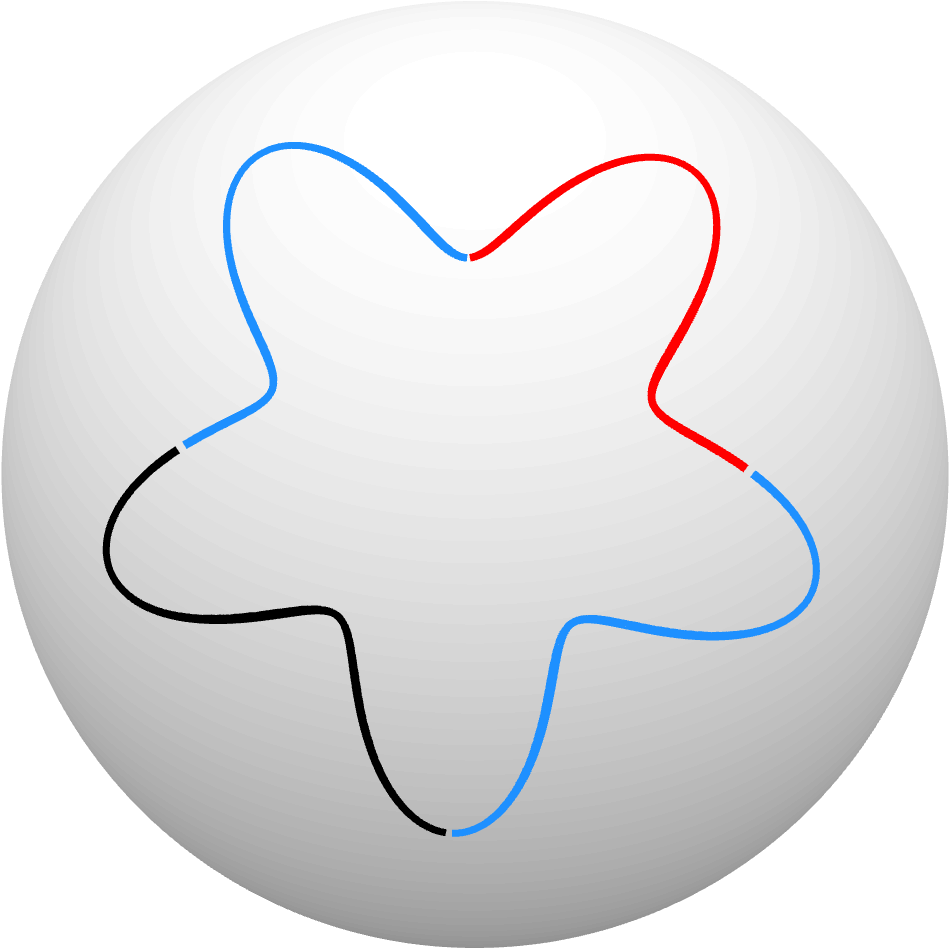
\includegraphics[width=\textwidth]{ContourLevel2}
                \caption{Level 2: \\ $\Gamma_4 \cup \Gamma_5 \cup \Gamma_6 \cup \Gamma_7$}
                \label{fig: ContourLevel2}
        \end{subfigure}
          \begin{subfigure}[b]{0.23\textwidth}
             \captionsetup{justification=centering}
                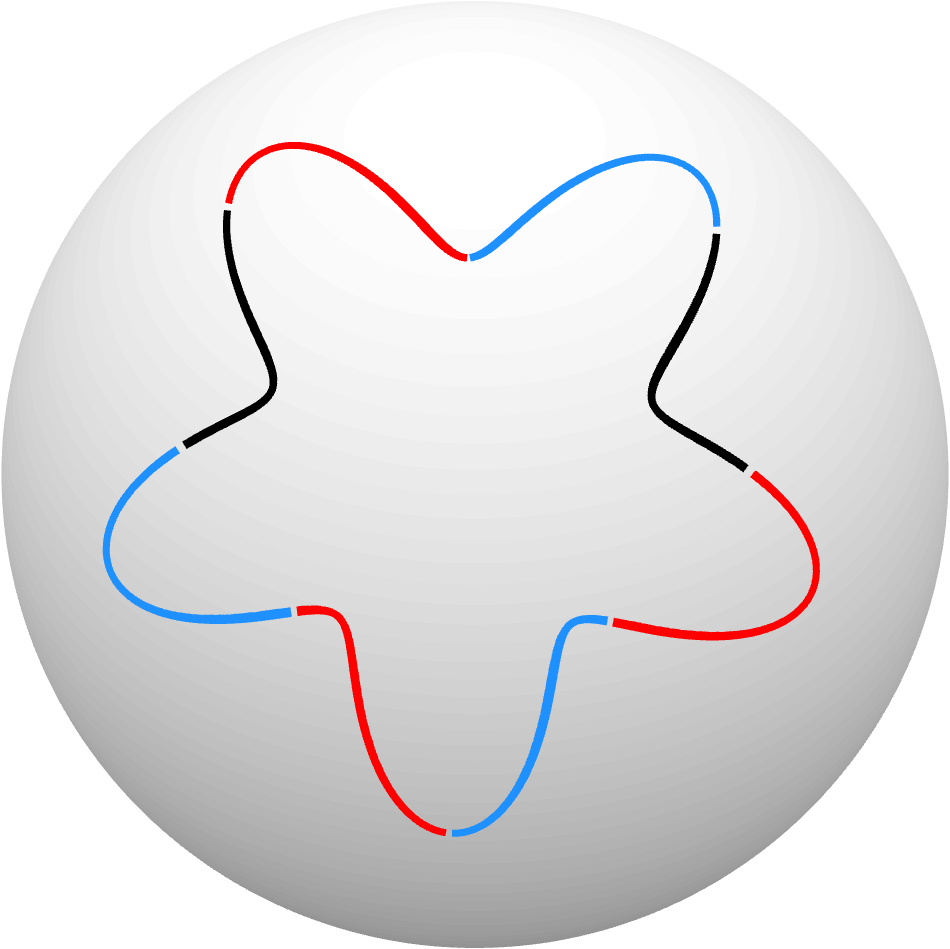
\includegraphics[width=\textwidth]{ContourLevel1}
                 \caption{Level 1: \\ $\Gamma_8 \cup \Gamma_9 \cup ... \cup \Gamma_{15} $}
                \label{fig: ContourLevel1}
        \end{subfigure}
        \caption{Binary tree placed on a star-shaped boundary, $\Gamma$. The subscripts correspond to the index vectors shown in the binary tree (\ref{eq: BinaryTree}). }
        \label{fig: ContourBinaryTree}
\end{figure}

%--------------------------------------------------------------------------------------------------------------------------------------------------------------------------------------------------------------------------------------

\subsubsection{Level 1}
The recursive algorithm begins on the finest level, $l=1$, where $p_1=8$ and $n_1=50$. We compress the horizontal and vertical off-diagonal blocks just as for single level compression. The first horizontal off-diagonal block is denoted by $A(I_8, L_8)$, where the index vectors $I_8$ and $L_8$, now correspond to those shown in the binary tree (\ref{eq: BinaryTree}). The row ID is then applied, giving 
\begin{align}
	&\hspace{2.3cm}\underset{n_1 \times (p_1-1)n_1}{A(I_8, L_8)}\approx\underset{ \ n_1 \times k_1 \ }{U_8} \underset{ \ k_1 \times  (p_1-1)n_1 \ } {S_{R_8},} \nonumber\\   
	&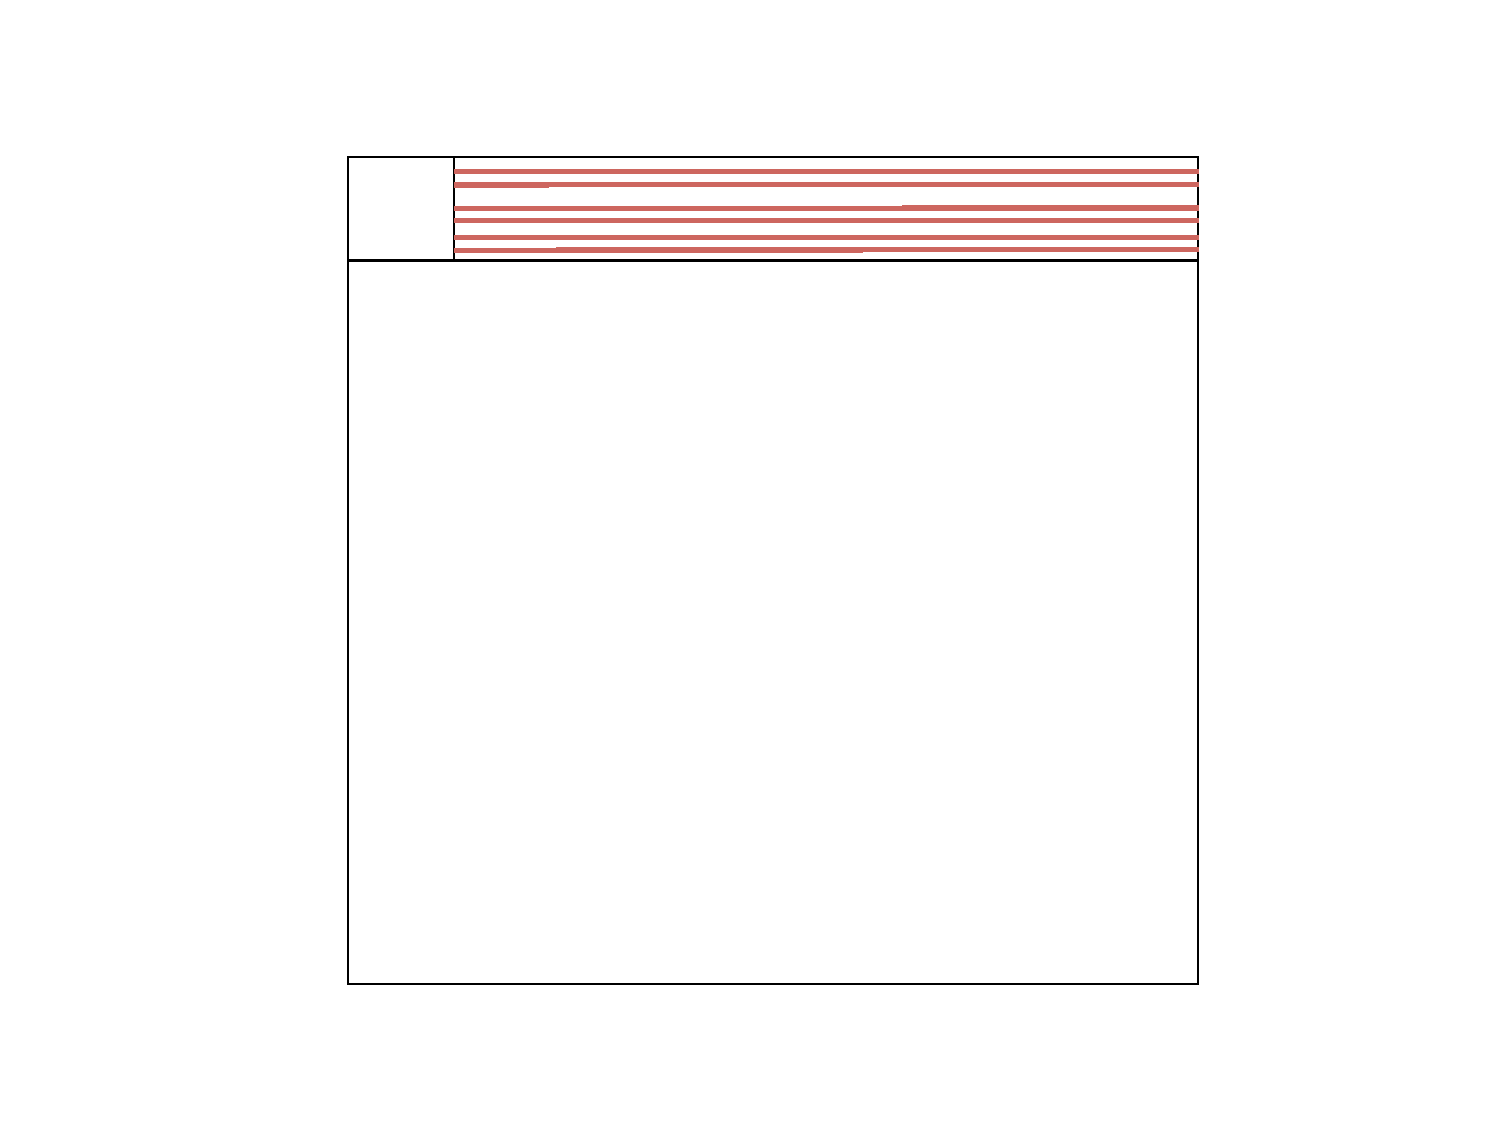
\includegraphics[width=0.3\textwidth]{BFRecLev1HorBlock8} \hspace{1cm} 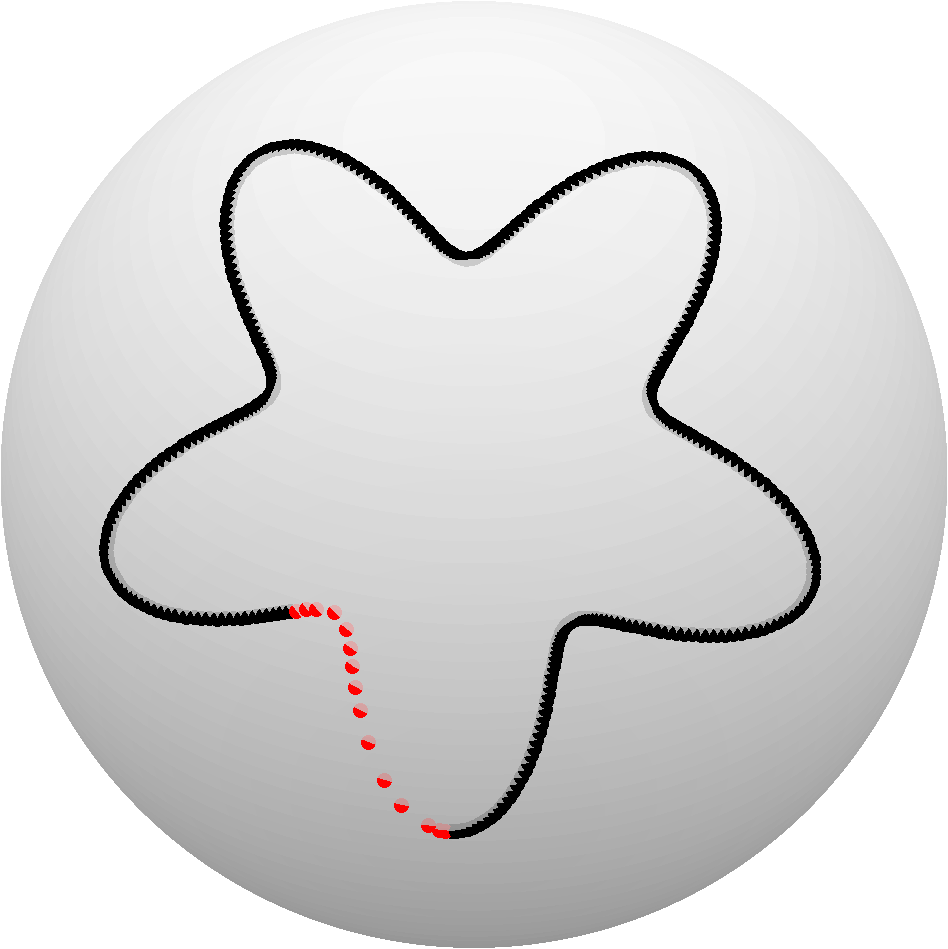
\includegraphics[width=0.3\textwidth]{BFRecLev1HorSkel8} \label{eq: BFRecLev1HorBlock8}
\end{align}
where $S_{R_8}$ is shown on the left. As with single-level compression we assume that on each level all horizontal and vertical off-diagonal blocks have the same rank, which is denoted by $k_1$ on level 1. The accuracy for the ID is set to $\varepsilon=10^{-5}$ across all levels in this example.

We recall from Section \ref{sec: Nystrom}, equation (\ref{eq: NystSystem}), that the matrix $A(I_8, L_8)$ represents the discretized kernel, 
\begin{align*}
	A(I_8, L_8)=\frac{h}{\pi}K(\mathbf{r}_i, \mathbf{r}_j), \quad i\in I_8, \ j\in L_8.
\end{align*}
Thus, selecting $k_1$ rows of $A(I_8, L_8)$, corresponds to evaluating $K(\mathbf{r}_i, \mathbf{r}_j)$ at $k_1$ points along $\mathbf{r}_i$. These $k_1$ skeleton points along $\Gamma_8$, are plotted in red in (\ref{eq: BFRecLev1HorBlock8}). Thus the ID can be thought of as reducing the number of rows in an off-diagonal block of $A$, or reducing the number of points needed to discretize the corresponding section of the boundary, $\Gamma_8$.  

The same steps are applied to the remaining 7 horizontal blocks on level 1. ID compression of each row block identifies $k_1$ skeleton points on $\Gamma_9$, ..., $\Gamma_{15}$. These are shown in Figure \ref{fig: BFRecLev1HorSkeleton}.
\begin{figure}[h]
	\centering
  	\begin{subfigure}[b]{0.24\textwidth}
  	\captionsetup{justification=centering}
    		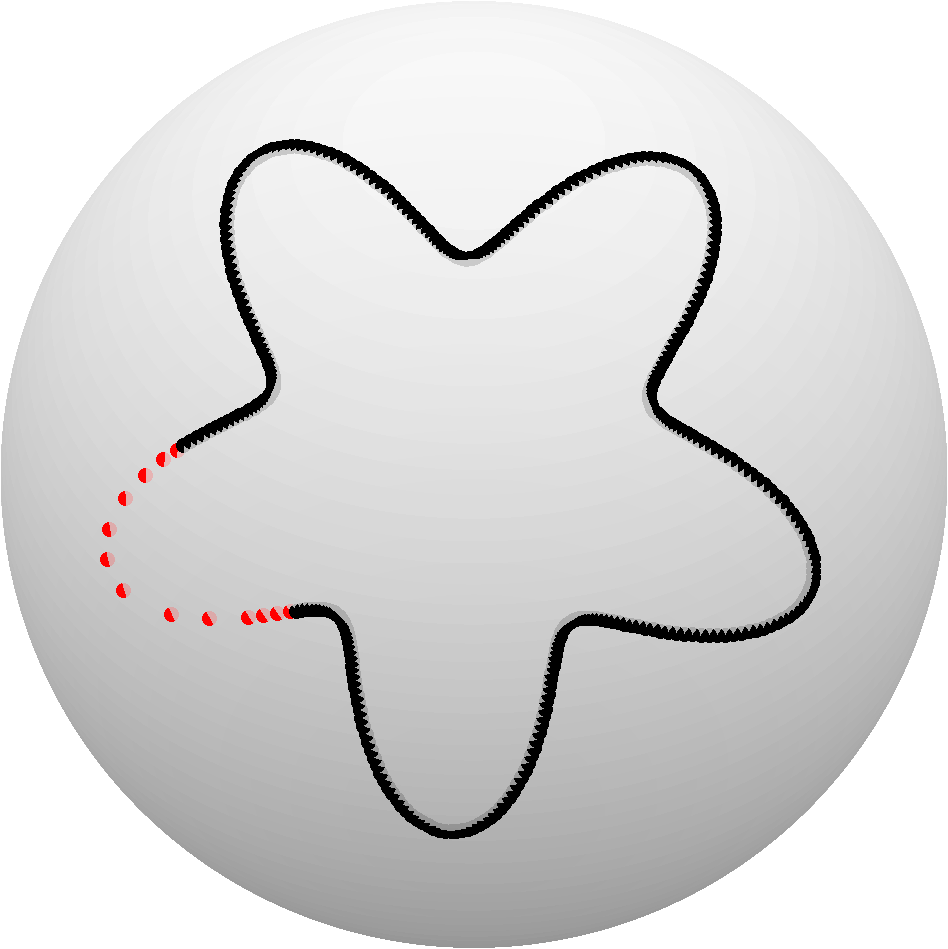
\includegraphics[width=\textwidth]{BFRecLev1HorSkel9}
    		\caption{Skeleton points for $\Gamma_9$.} 
       \end{subfigure}
       \quad
       \begin{subfigure}[b]{0.24\textwidth}
       \captionsetup{justification=centering}
      		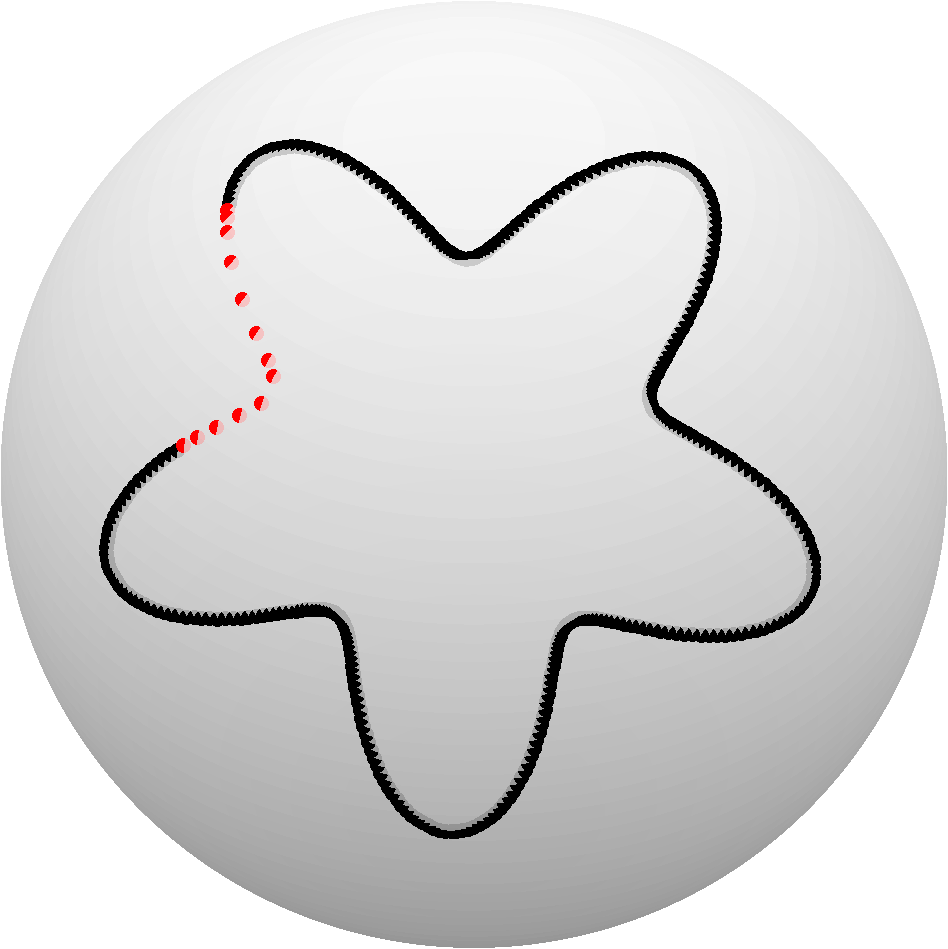
\includegraphics[width=\textwidth]{BFRecLev1HorSkel10}
    		\caption{Skeleton points for $\Gamma_{10}$.} 
       \end{subfigure}
       \hspace{1cm}
       \begin{subfigure}[t]{0.18\textwidth}
      		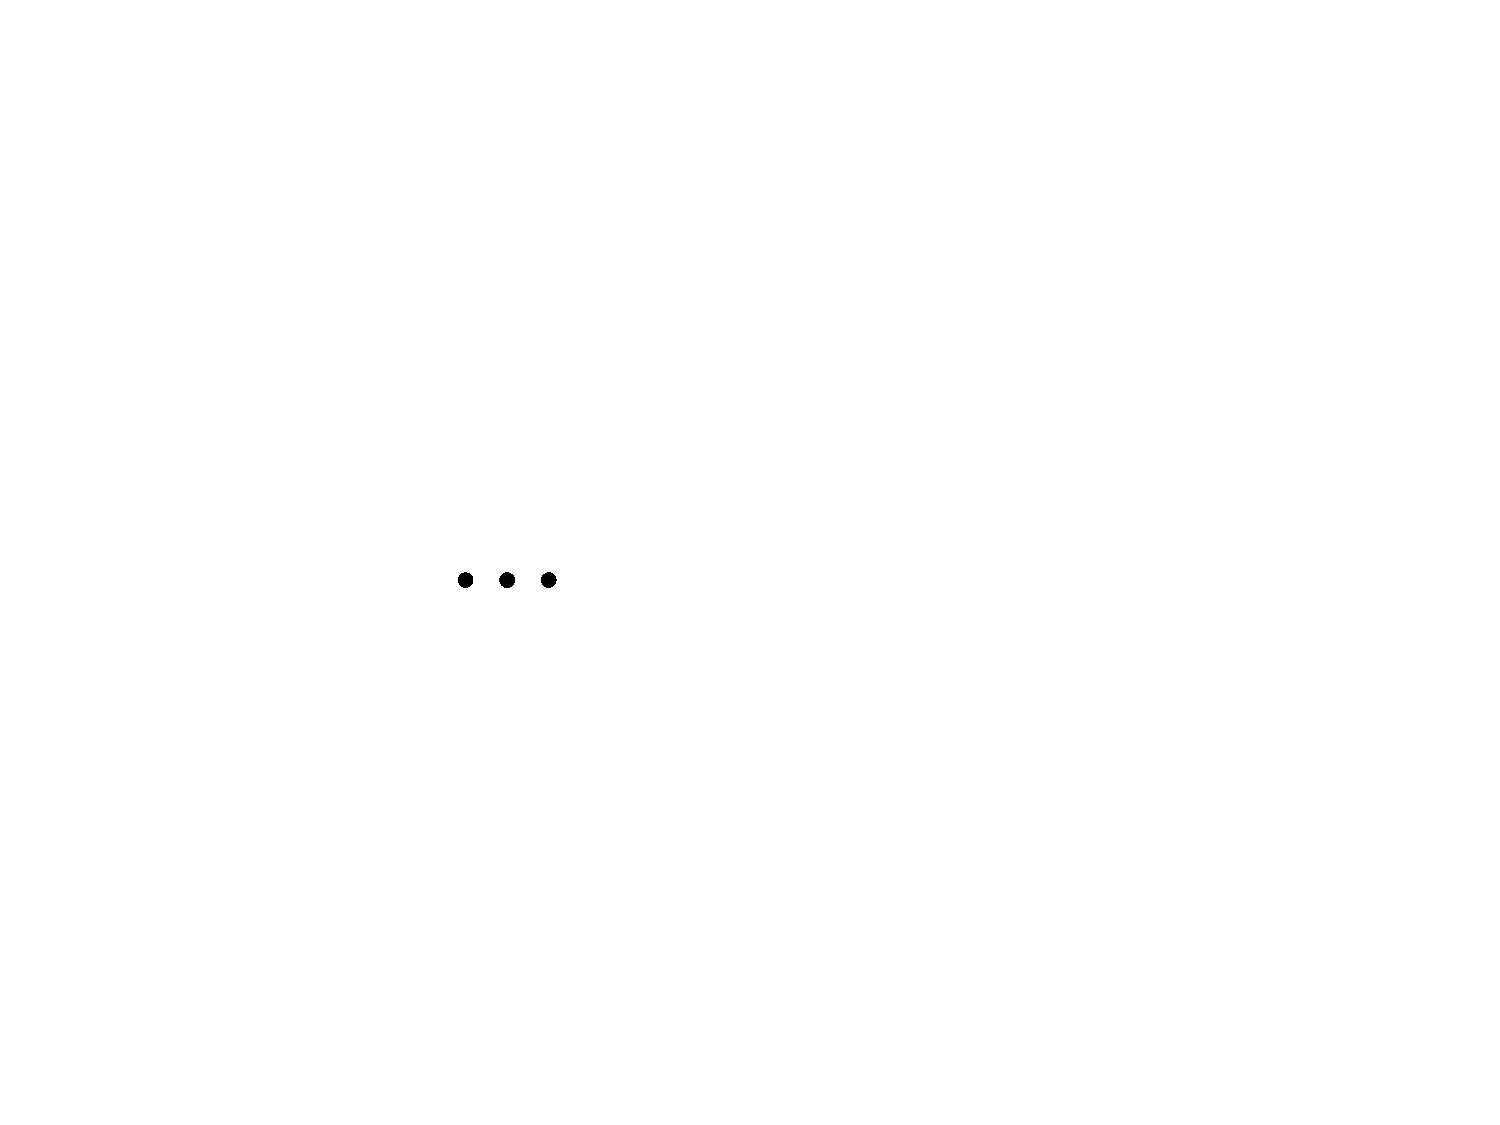
\includegraphics[width=0.7cm]{dots2}
      \end{subfigure}
      \hspace{-0.8cm}
     \begin{subfigure}[b]{0.24\textwidth}
     \captionsetup{justification=centering}
      		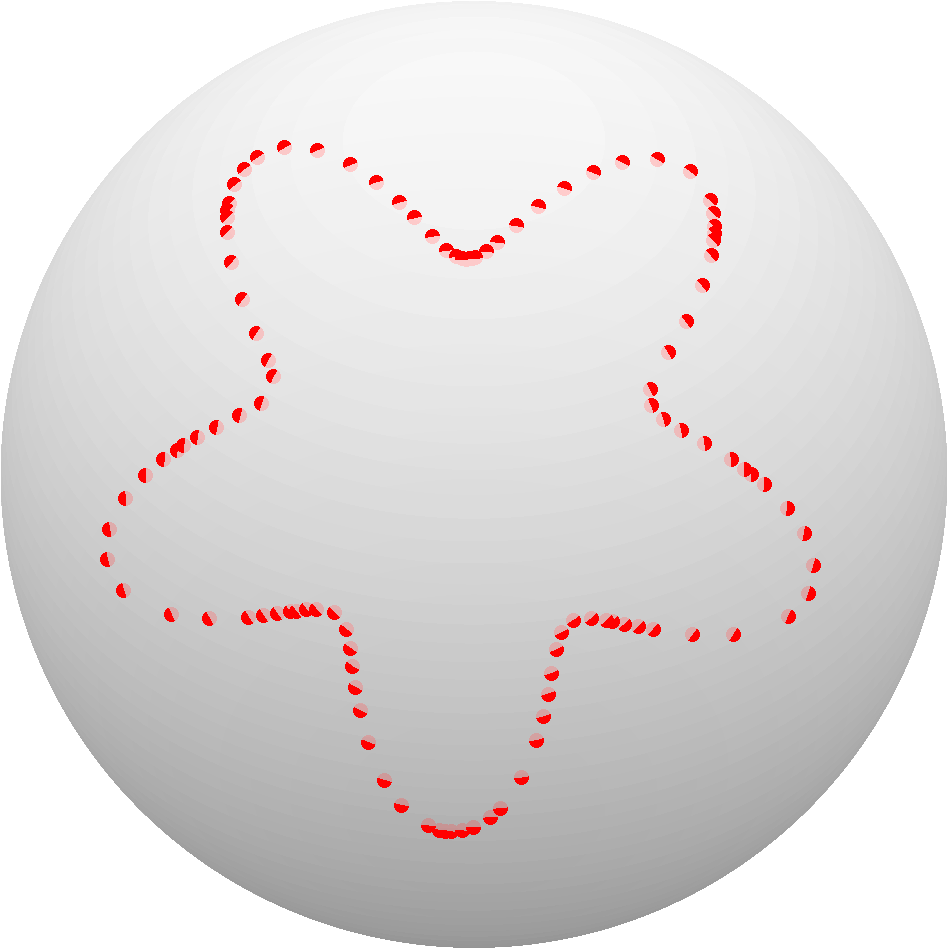
\includegraphics[width=\textwidth]{BFRecLev1HorSkelAll}
    		\caption{Skeleton points for $\Gamma_8$, ..., $\Gamma_{15}$.} 
      \end{subfigure}
      \caption{Skeleton points on level 1 for the second and third off-diagonal row blocks corresponding to $\Gamma_9$ and $\Gamma_{10}$ are shown in red. The accuracy of the ID is set to $\varepsilon=10^{-5}$. After compressing all off-diagonal row blocks, we obtain (c), which plots the skeleton points for $\Gamma_8$, ..., $\Gamma_{15}$. }
	\label{fig: BFRecLev1HorSkeleton}
\end{figure}
       
The same procedure can be applied to the $p_1=8$ vertical blocks of $A$ to give a new set of skeleton points on $\Gamma_8, ..., \Gamma_{15}$. The ID for the first off-diagonal column block is given by
\begin{align*}
	&\hspace{2.3cm}\underset{(p_1-1)n_1 \times n_1 }{A(L_8, I_8)}\approx\underset{ \ (p_1-1)n_1 \times k_1 \ }{S_{C_8}} \underset{ \ k_1 \times n_1 \ } {V_8^*},  \nonumber\\   
	&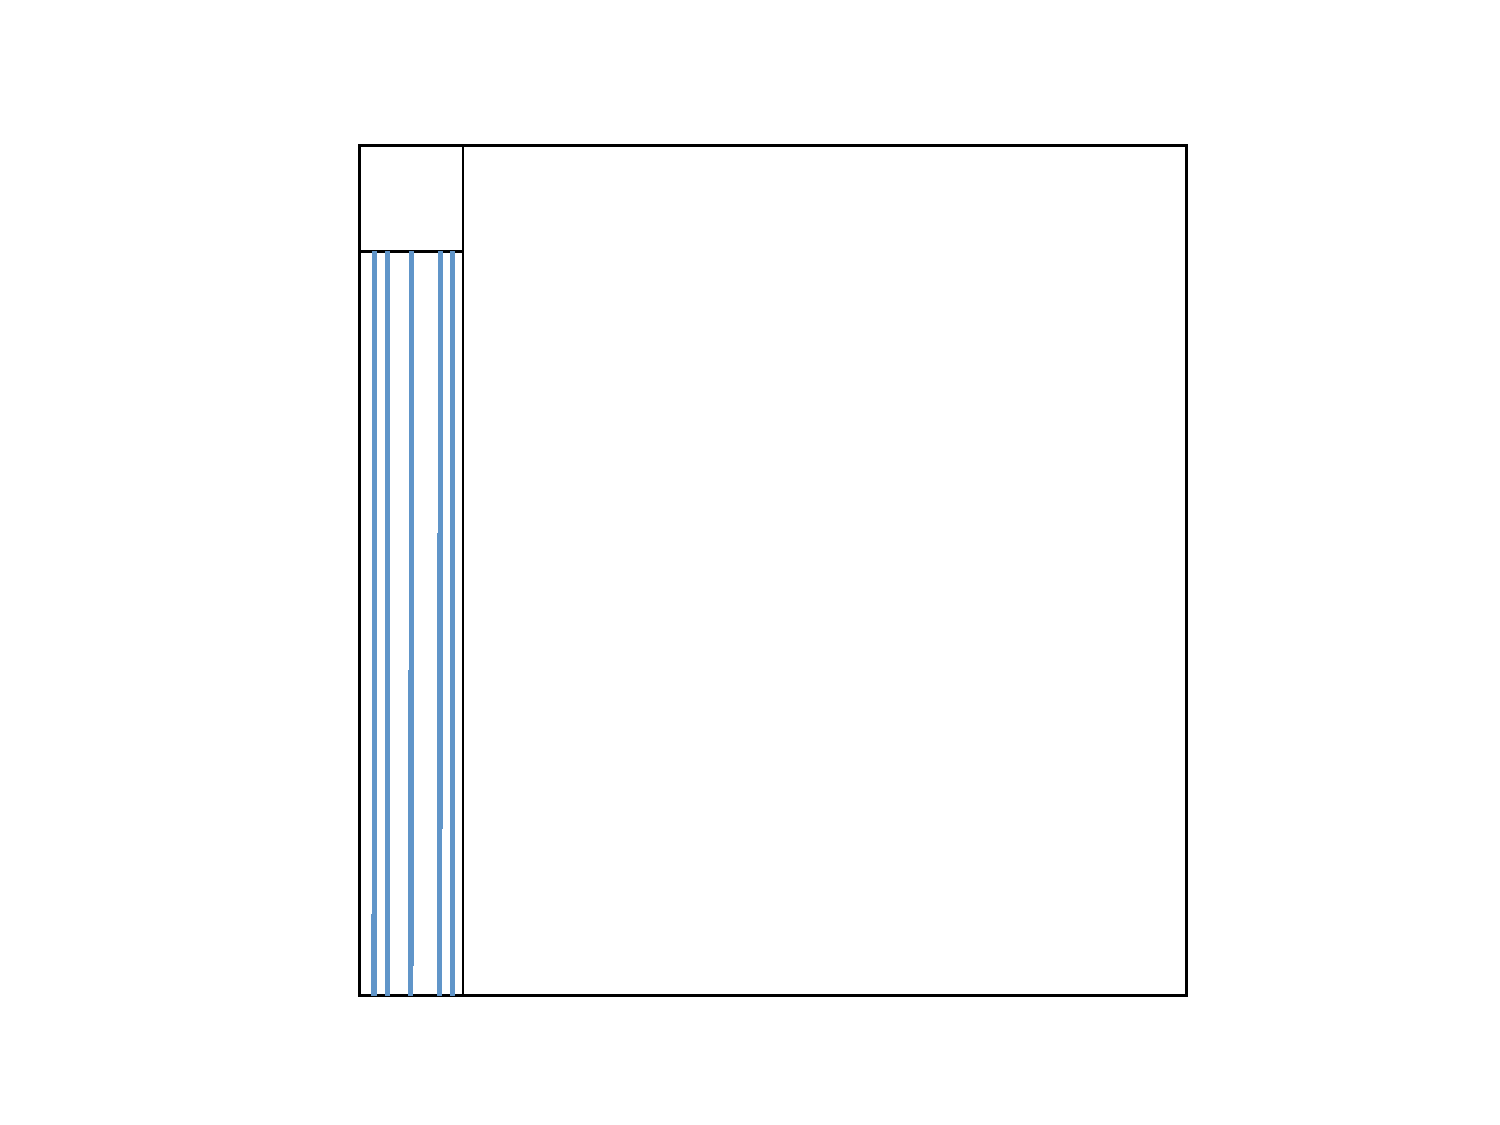
\includegraphics[width=0.3\textwidth]{BFRecLev1VerBlock8} \hspace{1cm} 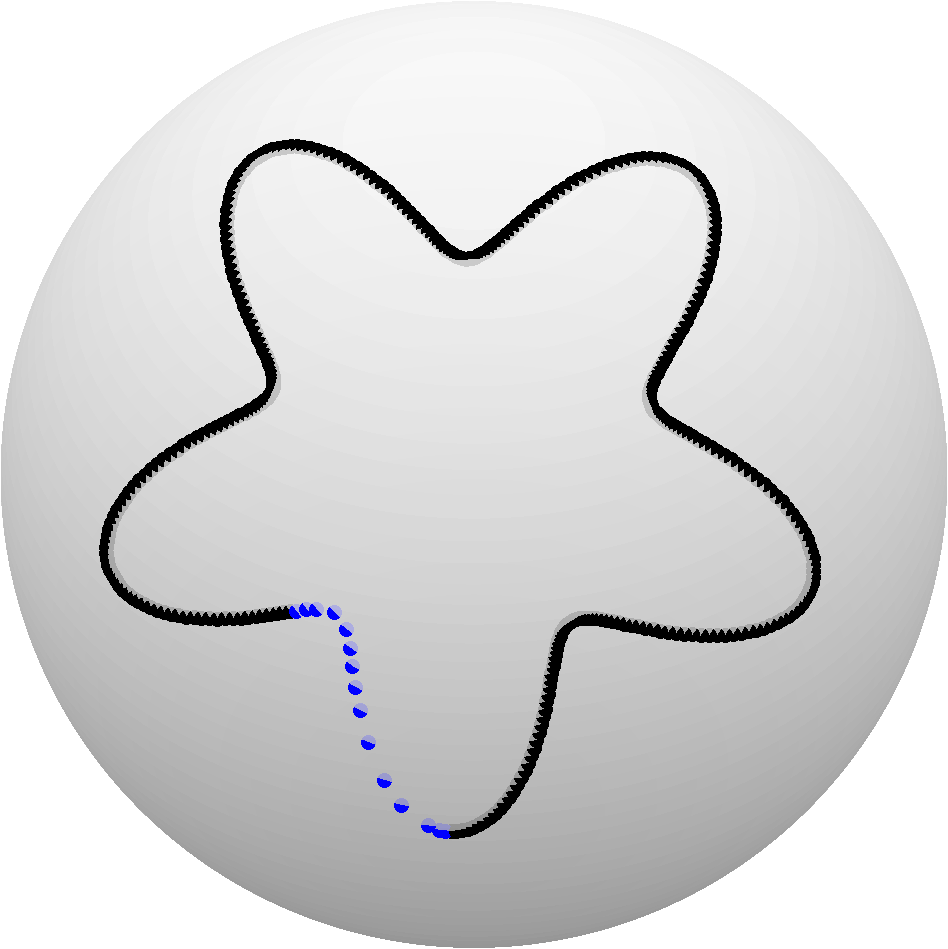
\includegraphics[width=0.3\textwidth]{BFRecLev1VerSkel8} 
\end{align*}
where $S_{C_8}$ is shown on the left. Selecting $k_1$ columns of $A(L_8, I_8)$ now corresponds to evaluating $K(\mathbf{r}_i, \mathbf{r}_j)$ at $\mathbf{r}_i$ using $k_1$ points along $\mathbf{r}_j$. 

However fast direct solvers typically compress the horizontal and vertical blocks at the same time \cite{GillYoungMart2012, MartRokh2005}. This means that for the $\tau^{th}$ horizontal and vertical off-diagonal blocks, the ID is applied to the matrix 
\begin{align*}
	&\hspace{0.2cm}\underset{n_1 \times 2(p_1-1)n_1}{\left[\begin{array}{c c}
	A(I_\tau, L_\tau) & A^*(L_\tau, I_\tau)
\end{array}\right]}.\\
	&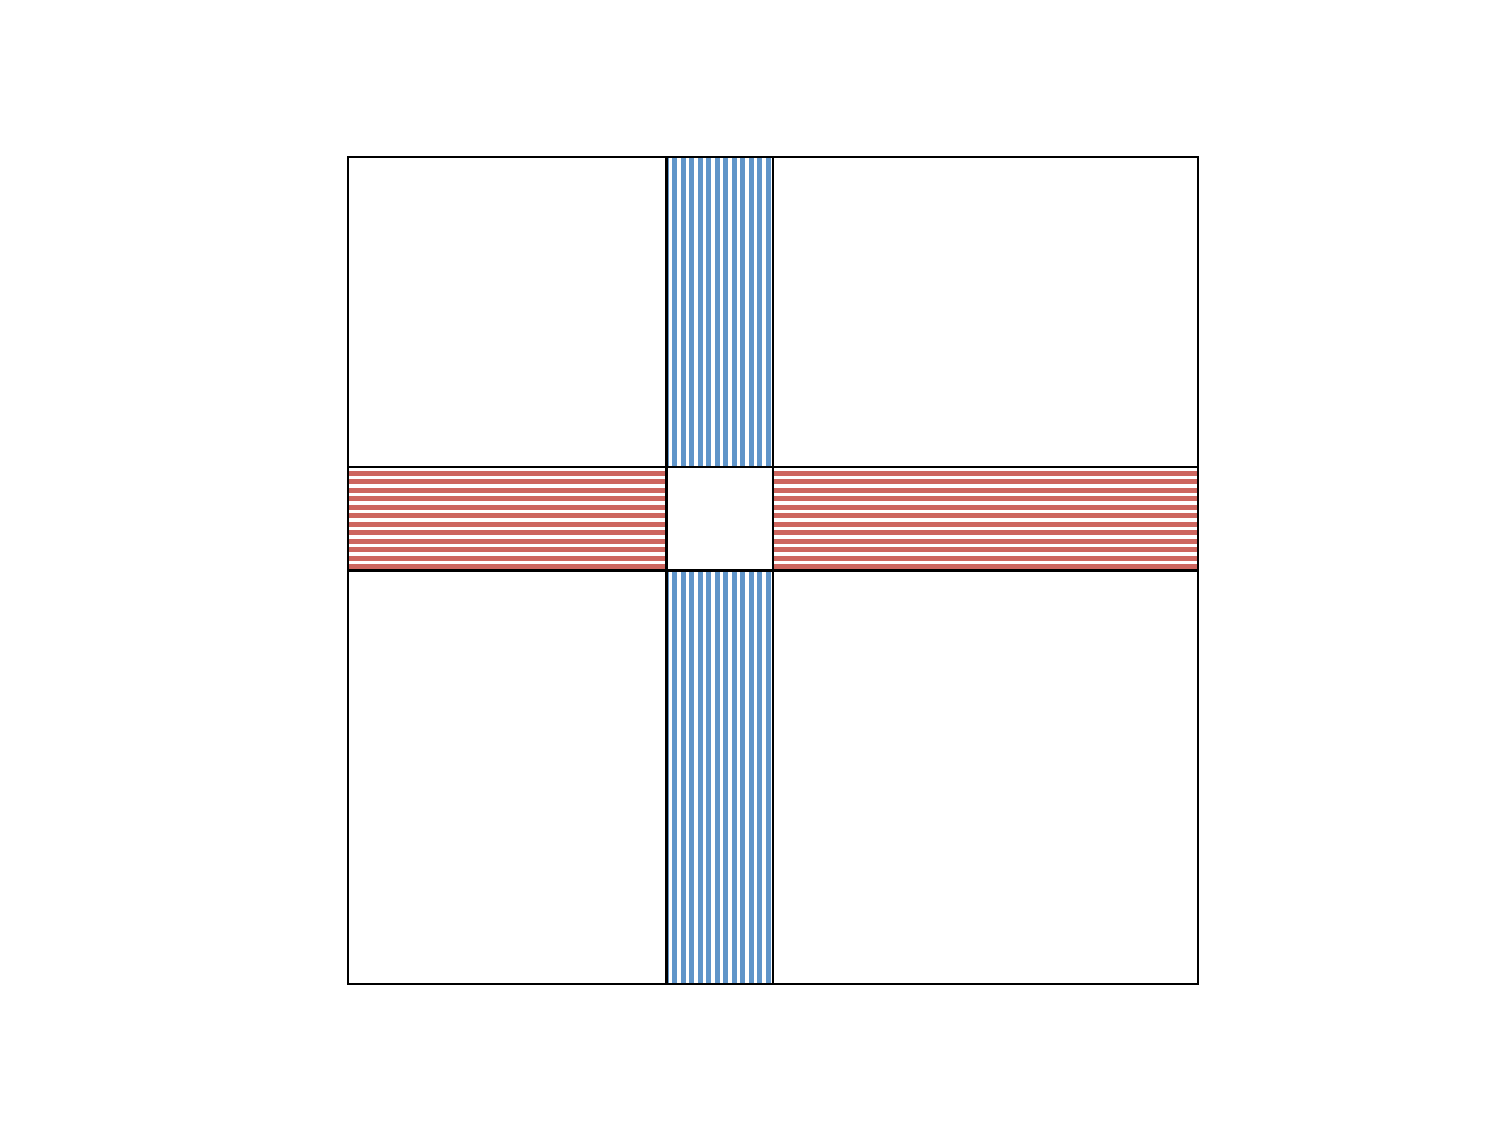
\includegraphics[width=0.3\textwidth]{BFRecLev1HorVerBlockTau}
\end{align*}

In this way the resulting row and column skeletons are the same, with $U=V$. This has been noted to produce slightly higher ranks $k$, but leads to better stability of the compression and inversion stages \cite{MartRokh2005, GillYoungMart2012}.
If we apply this approach then we have the same set of skeleton points for both the rows ($\mathbf{r}_i$) and columns ($\mathbf{r}_j$). 

The resulting factorization for $A$ on this level is 
\begin{center}
	\begin{tabular}[t]{ccccccc}
	$\underset{8n_1 \times 8n_1}{A}$ & $\approx$ & $\underset{ \ 8n_1 \times 8k_1 \ }{U^{(1)}}$  &  $\underset{ \ 8k_1 \times 8k_1 \ }{S^{(1)}}$ & $\underset{ \ 8k_1 \times 8n_1 \ }{{(V^{(1)})}^*} $& + &$\underset{ \ 8n_1 \times 8n_1 \ }{D^{(1)}.}$ \\ [.4cm]
	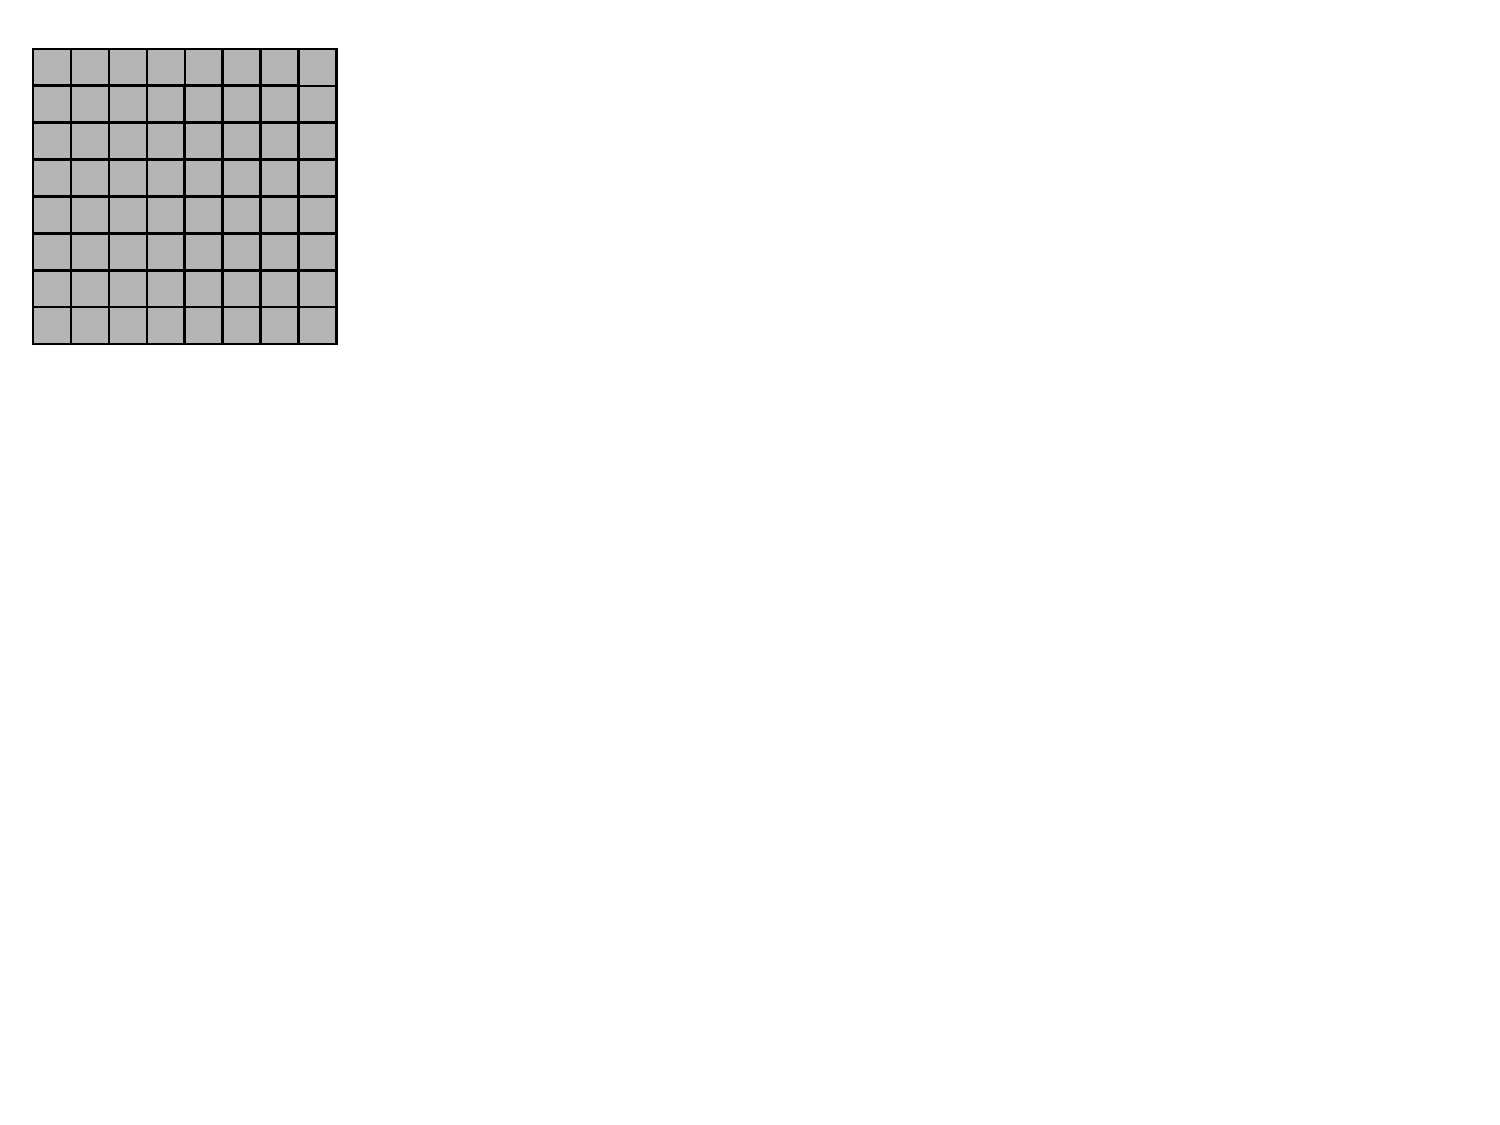
\includegraphics[width=3cm]{BFRecLev1A_8by8} & & 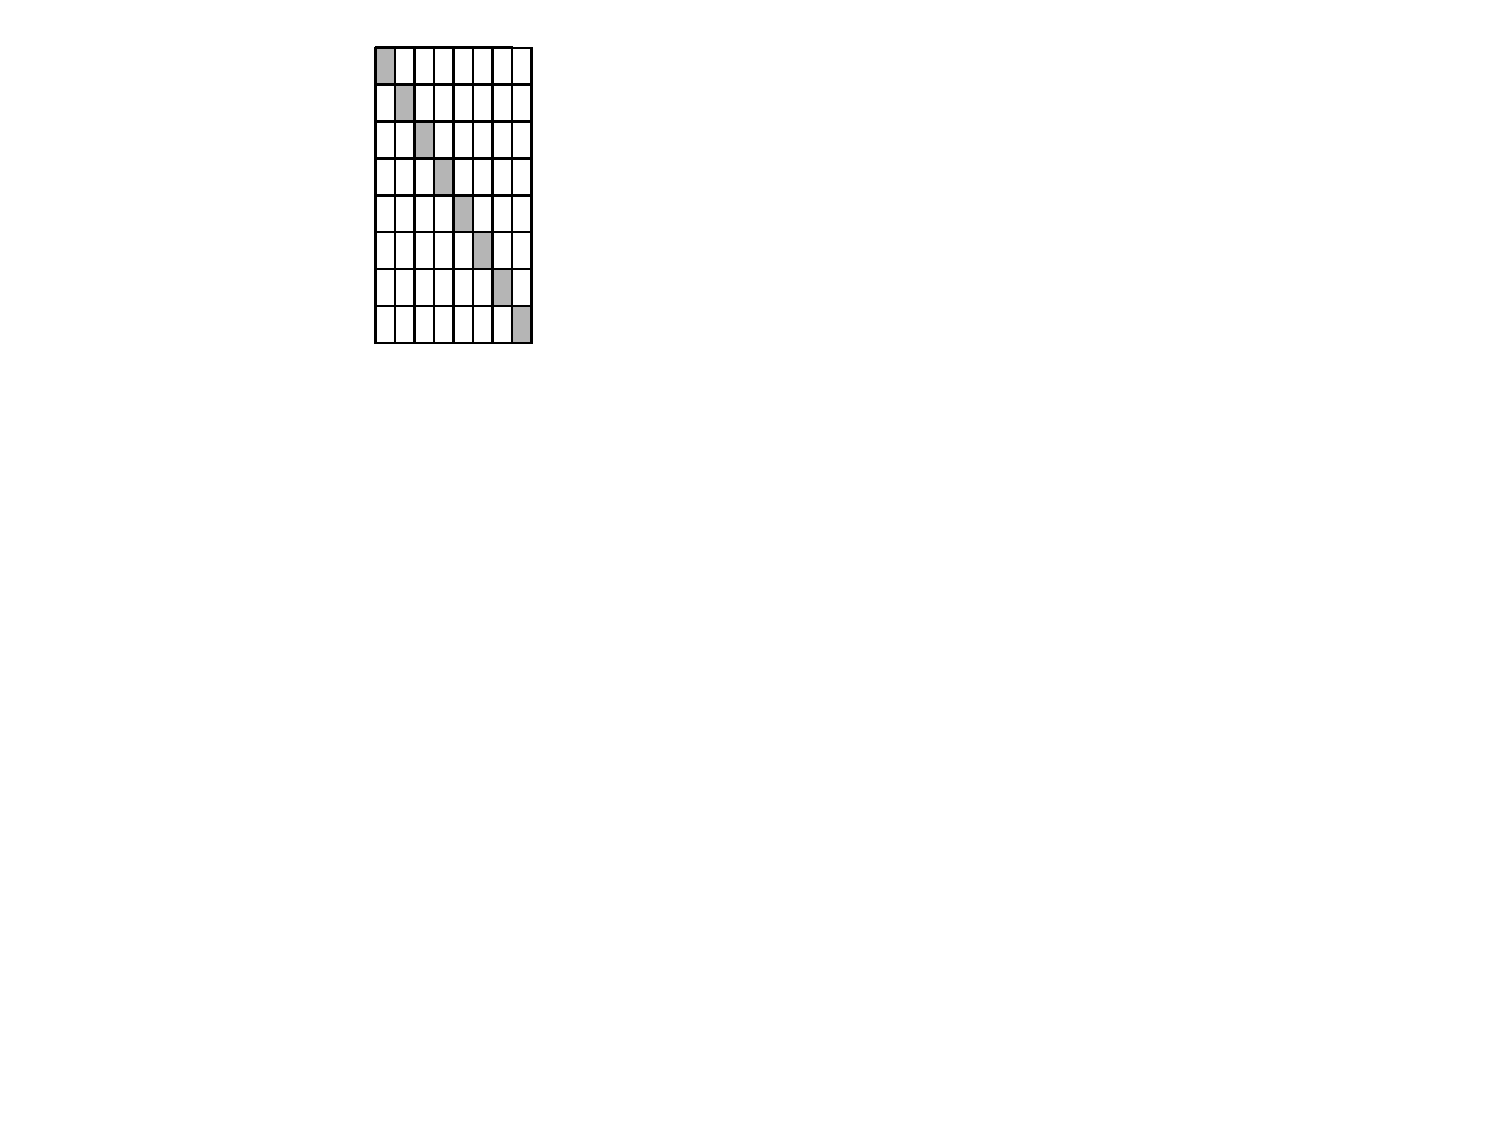
\includegraphics[width=1.58cm]{BFRecLev1U1} & 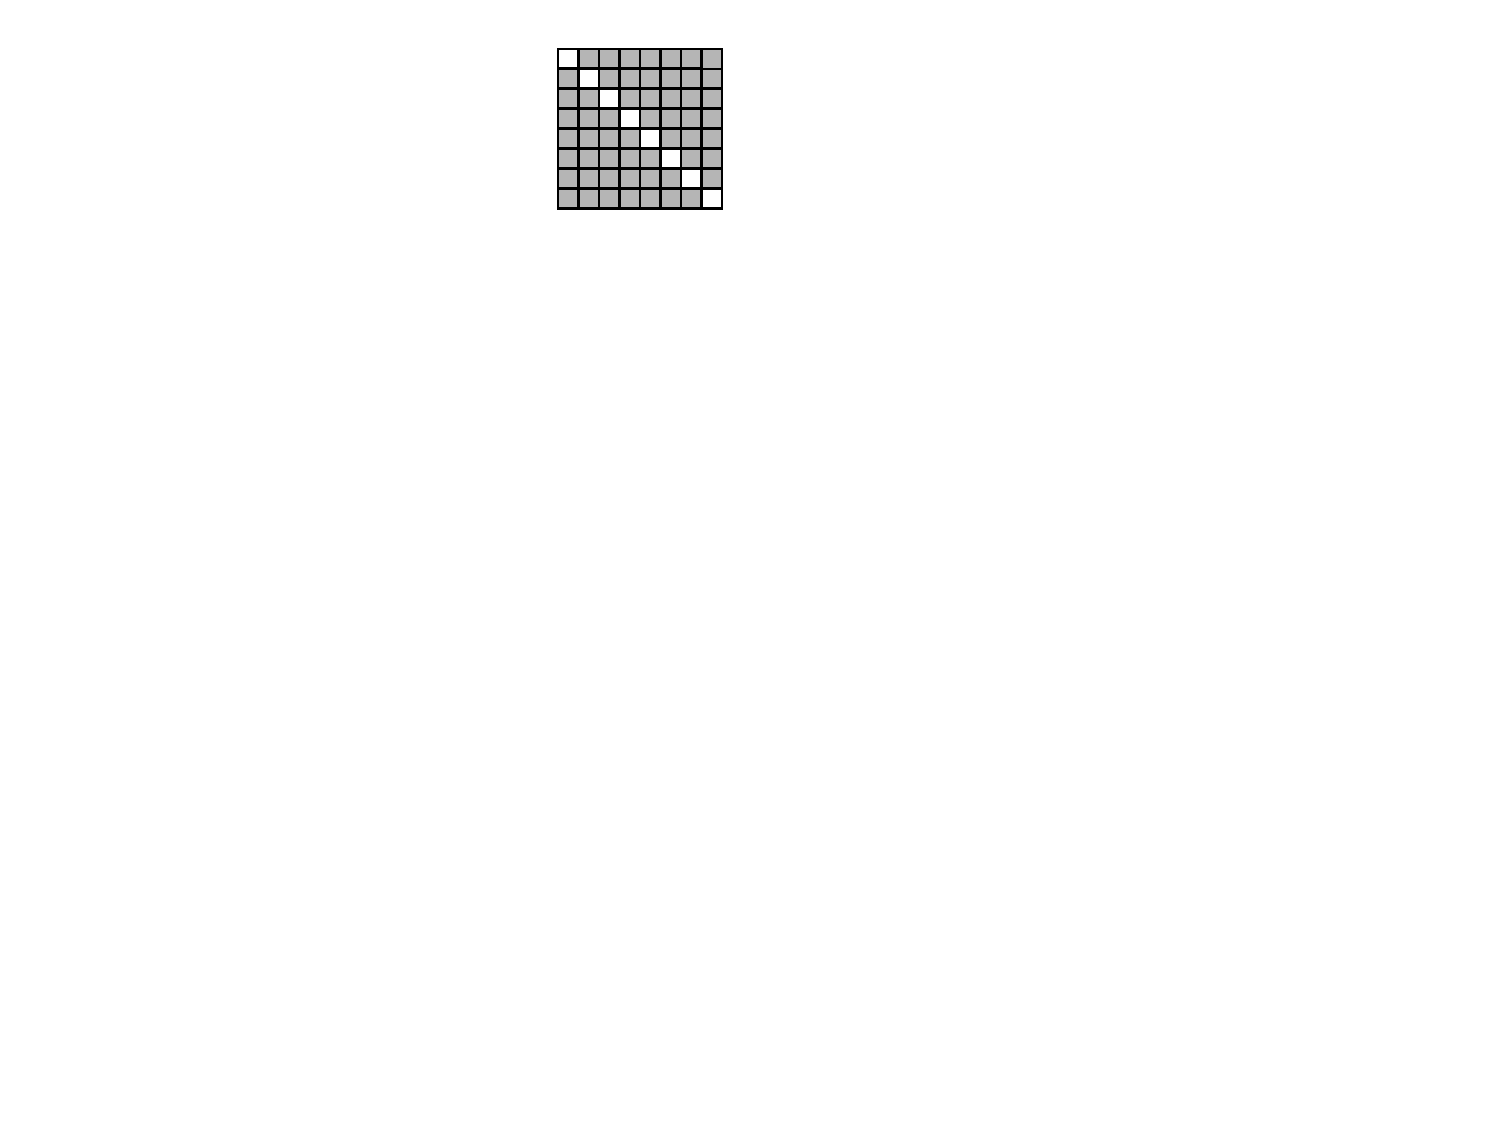
\includegraphics[width=1.68cm]{BFRecLev1S1} &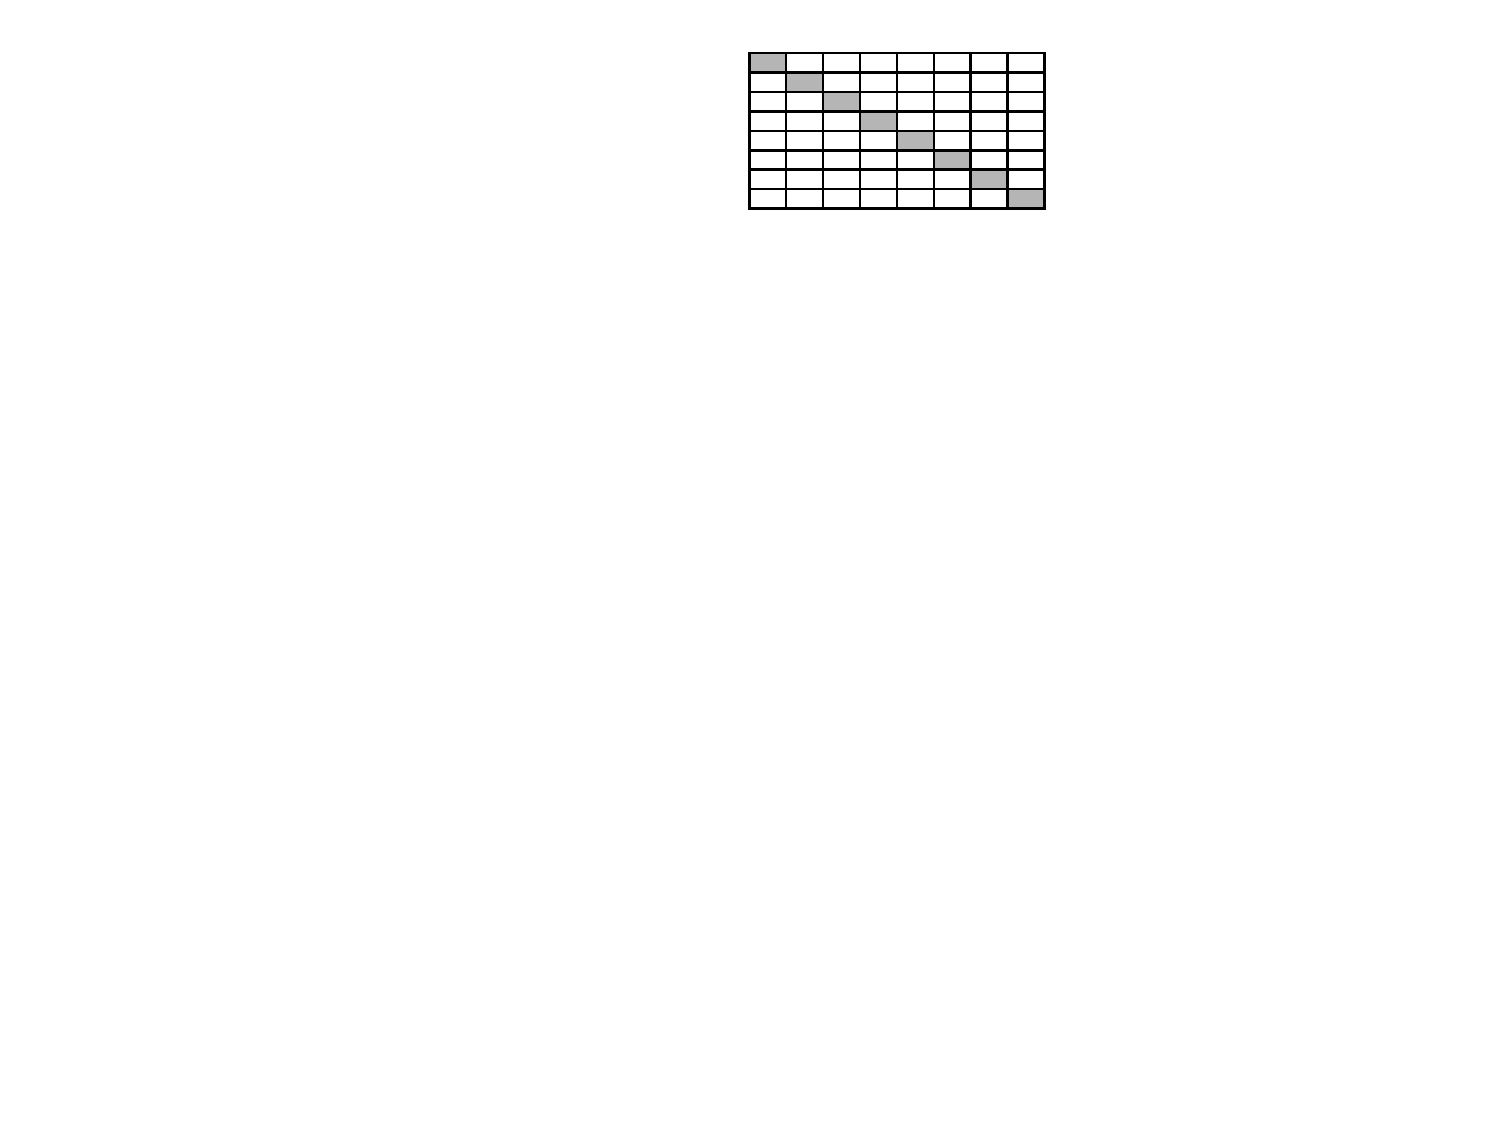
\includegraphics[width=3cm]{BFRecLev1V1} &  &  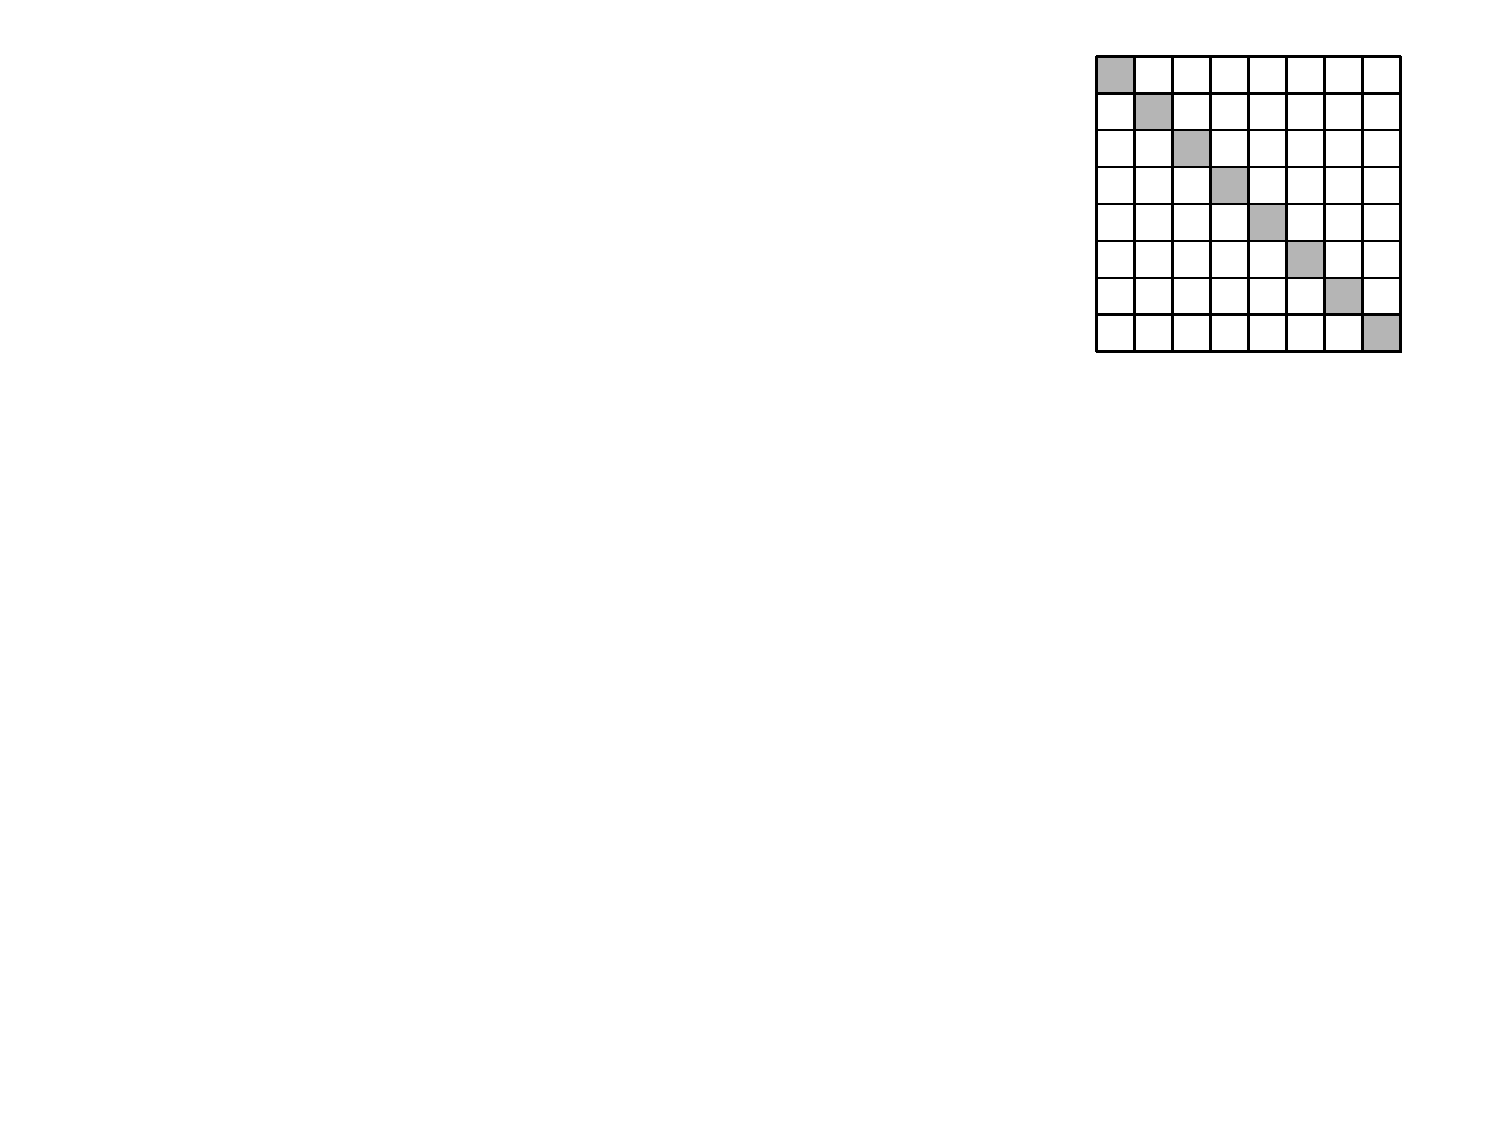
\includegraphics[width=3cm]{BFRecLev1D1} 
	\end{tabular}
\end{center}
The white and grey blocks indicate zero and nonzero entries in the matrices respectively.

Examining $S^{(1)}$ we see that it is also a dense matrix which when re-grouped into larger blocks has rank-deficient off-diagonal blocks. This means that the same single-level compression scheme can now be applied to $S^{(1)}$.

%--------------------------------------------------------------------------------------------------------------------------------------------------------------------------------------------------------------------------------------

\subsubsection{Level 2}
On level 2, we set $n_2=2k_1$, and $p_2=4$.  We then compress the matrix $S^{(1)}$ exactly as we would in the single-level compression scheme, except now the entries in the matrix correspond to the skeleton points selected on level 1 (Figure \ref{fig: BFRecLev1HorSkeleton}). If we let $\tilde{I}_\tau$ denote the indices of the skeletonized points from level 1, then the index vectors for the first off-diagonal blocks on level 2 are given by 
\begin{align*}
	I_4&=\tilde{I}_8 \cup \tilde{I}_9\\
	L_4&=\tilde{I}_{10}\cup...\cup \tilde{I}_{15}.
\end{align*} 
Applying the row ID to the first horizontal off-diagonal block we obtain 
\begin{align}
	&\hspace{2cm}\underset{n_2 \times (p_2-1)n_2}{S^{(1)}(I_4, L_4)}=\underset{ \ n_2 \times k_2 \ }{U_4} \underset{ \ k_2 \times (p_2-1)n_2 \ }{S_{R_4}.} \nonumber \\
	&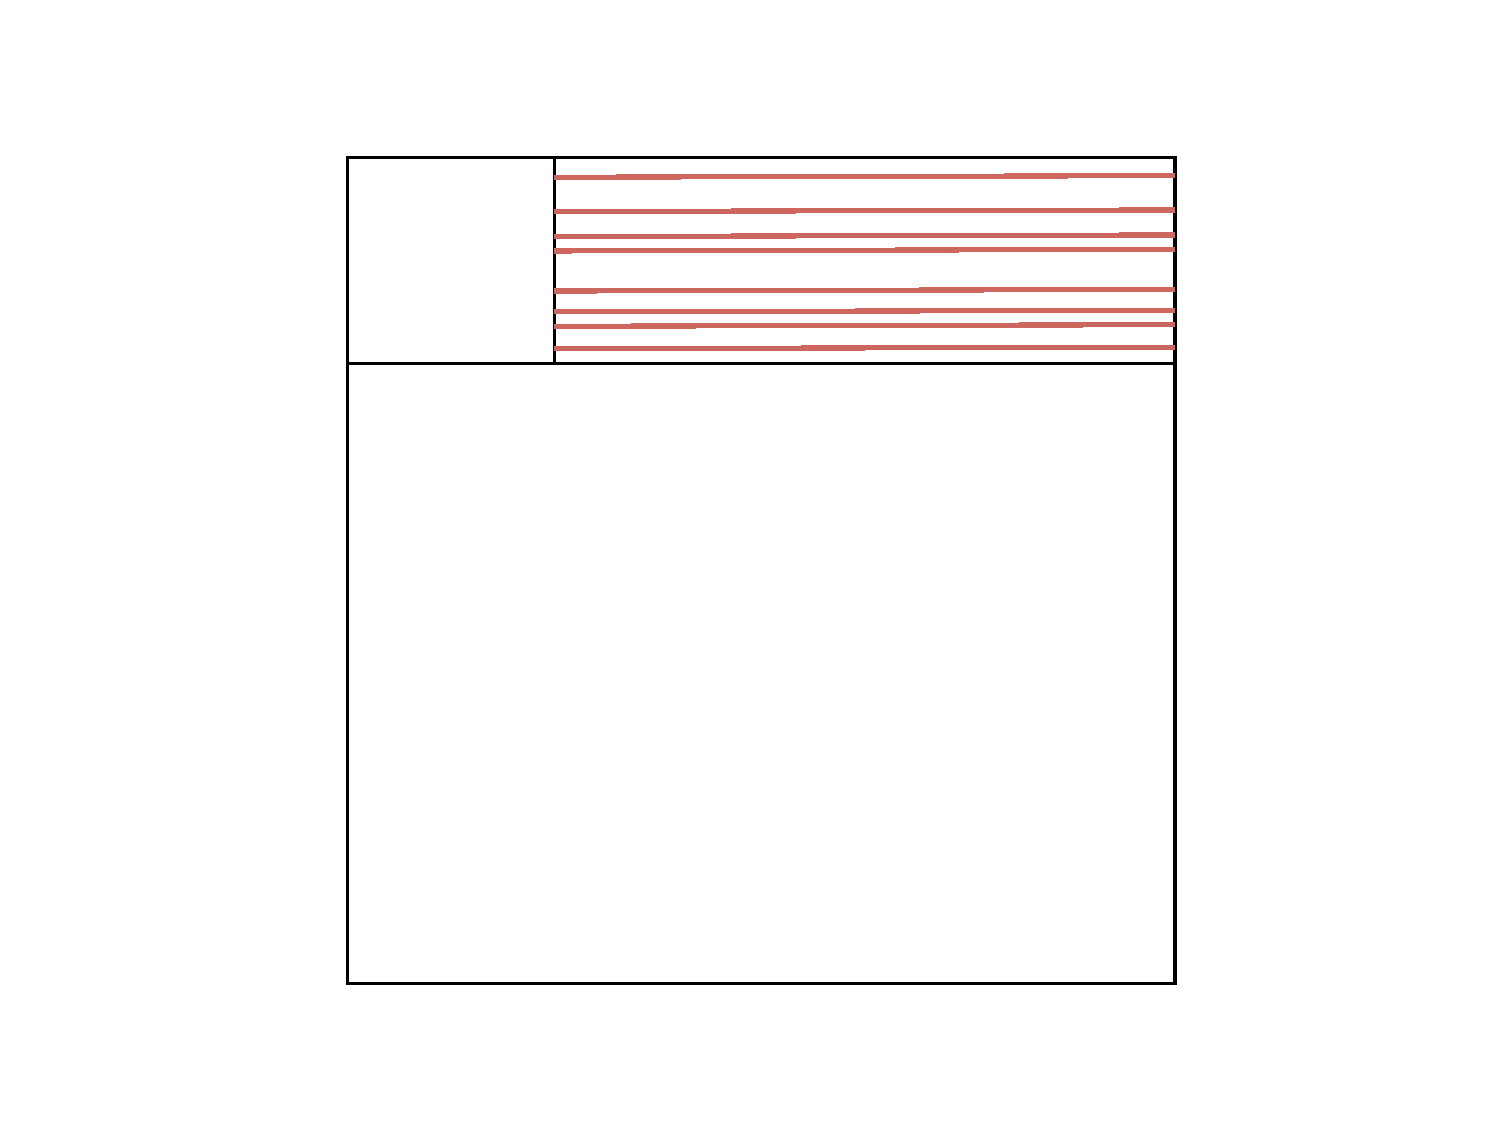
\includegraphics[width=0.24\textwidth]{BFRecLev2HorBlock4} \hspace{1cm} 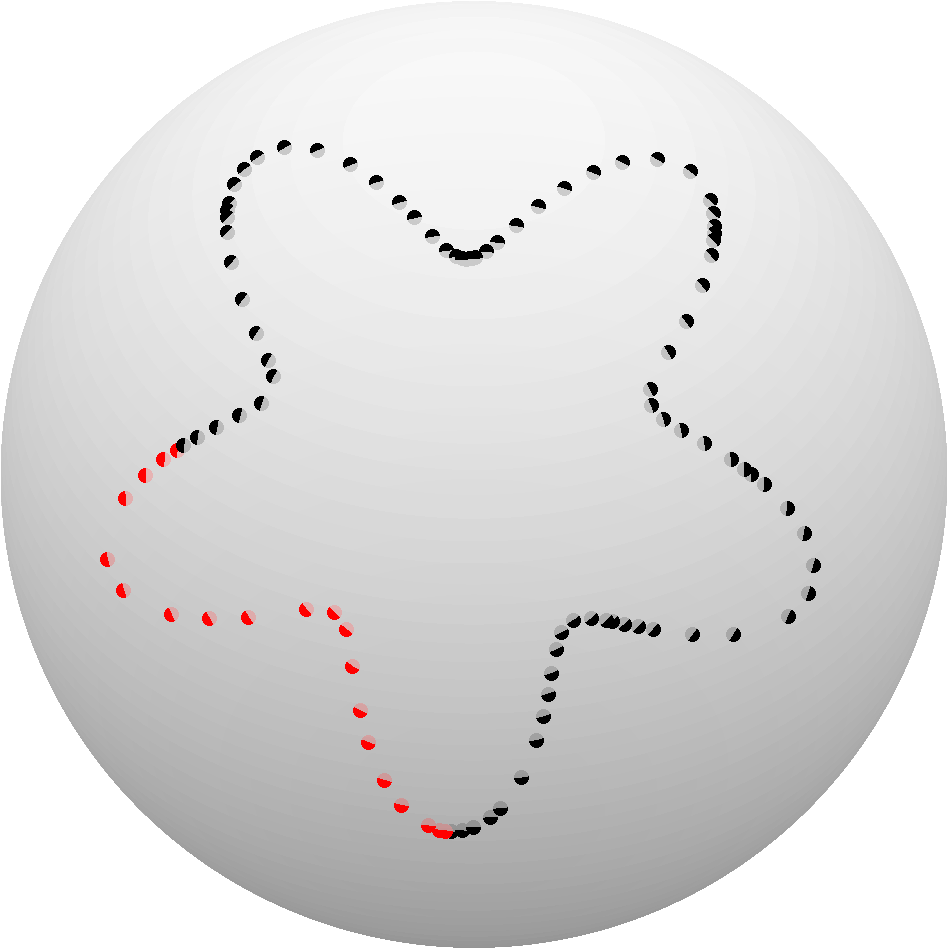
\includegraphics[width=0.3\textwidth]{BFRecLev2Skel4} \label{eq: BFRecLev2HorBlock4}
\end{align}
As mentioned previously, this is done simultaneously with the off-diagonal column $S^{(1)}(L_4, I_4)$ to obtain a matching column skeleton. Applying the ID to the remaining off-diagonal blocks on this level, we obtain the skeleton points shown in Figure \ref{fig: BFRecLev2Skeleton}. 
\begin{figure}[h]
	\centering
	\begin{subfigure}[b]{0.24\textwidth}
	\captionsetup{justification=centering}
		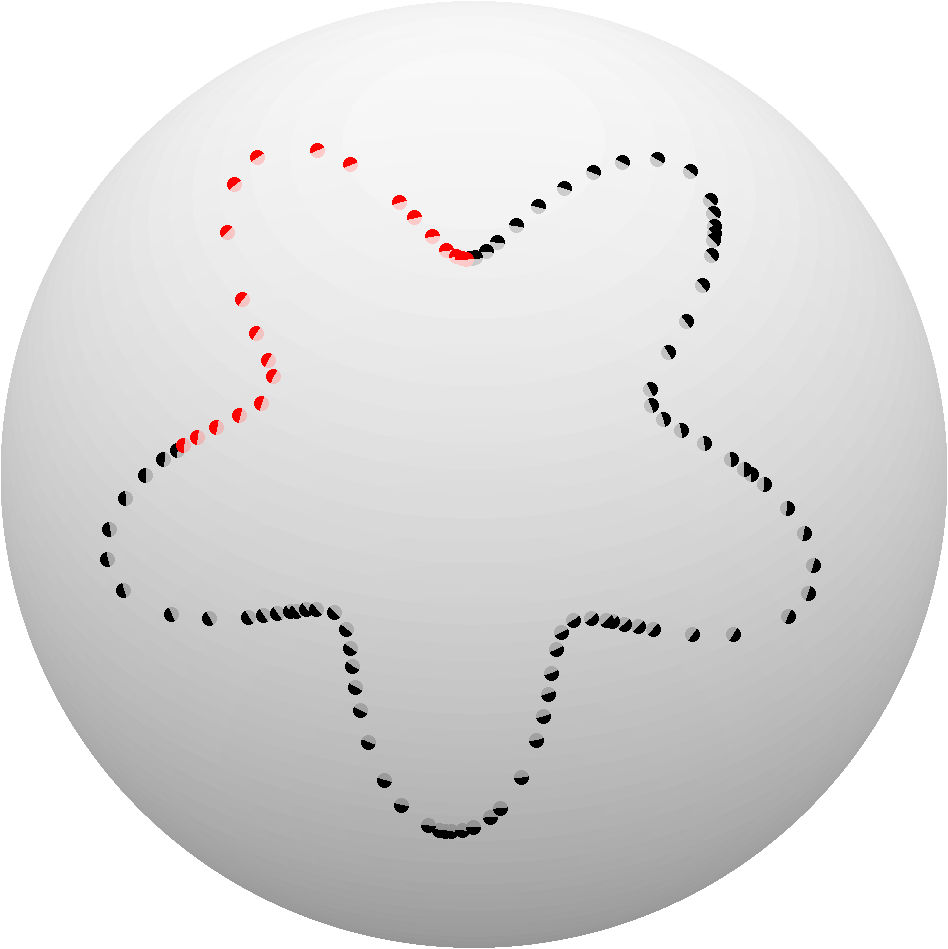
\includegraphics[width=\textwidth]{BFRecLev2Skel5}
    		\caption{Skeleton points for $\Gamma_5$.} 
       \end{subfigure}
       \quad
       \begin{subfigure}[b]{0.24\textwidth}
       \captionsetup{justification=centering}
      		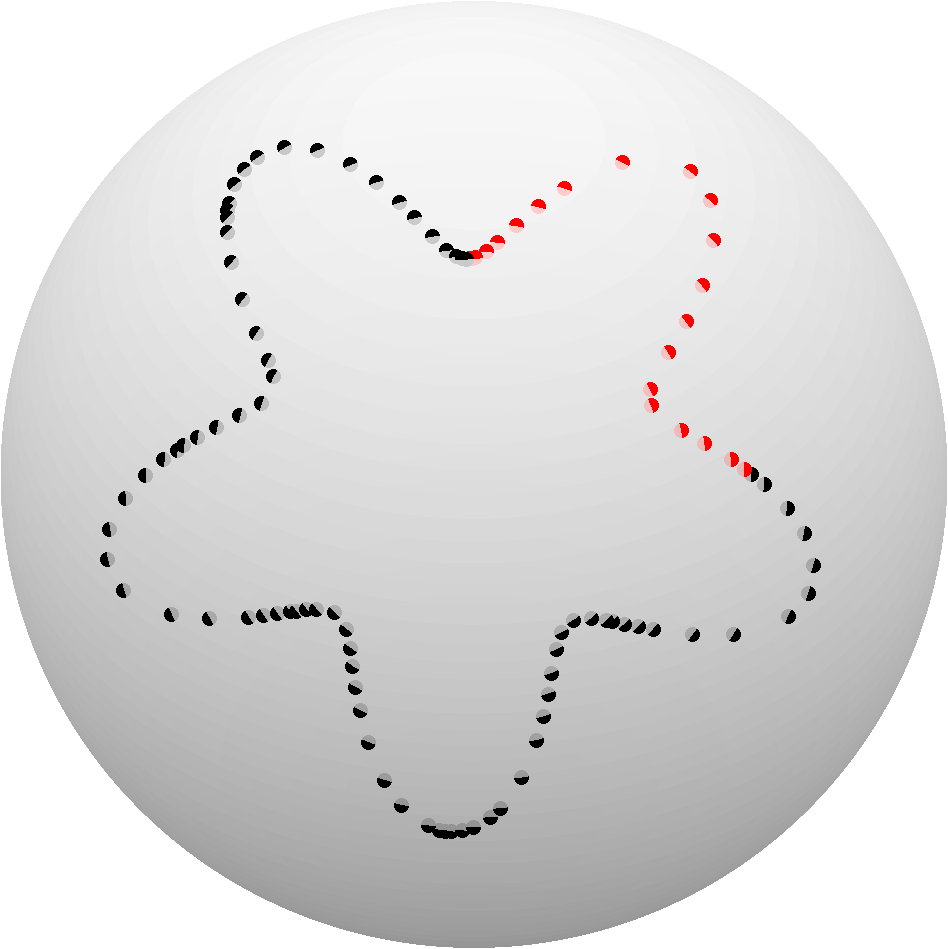
\includegraphics[width=\textwidth]{BFRecLev2Skel6}
    		\caption{Skeleton points for $\Gamma_{6}$.} 
     \end{subfigure}
     \hspace{1cm}
      \begin{subfigure}[t]{0.18\textwidth}
      		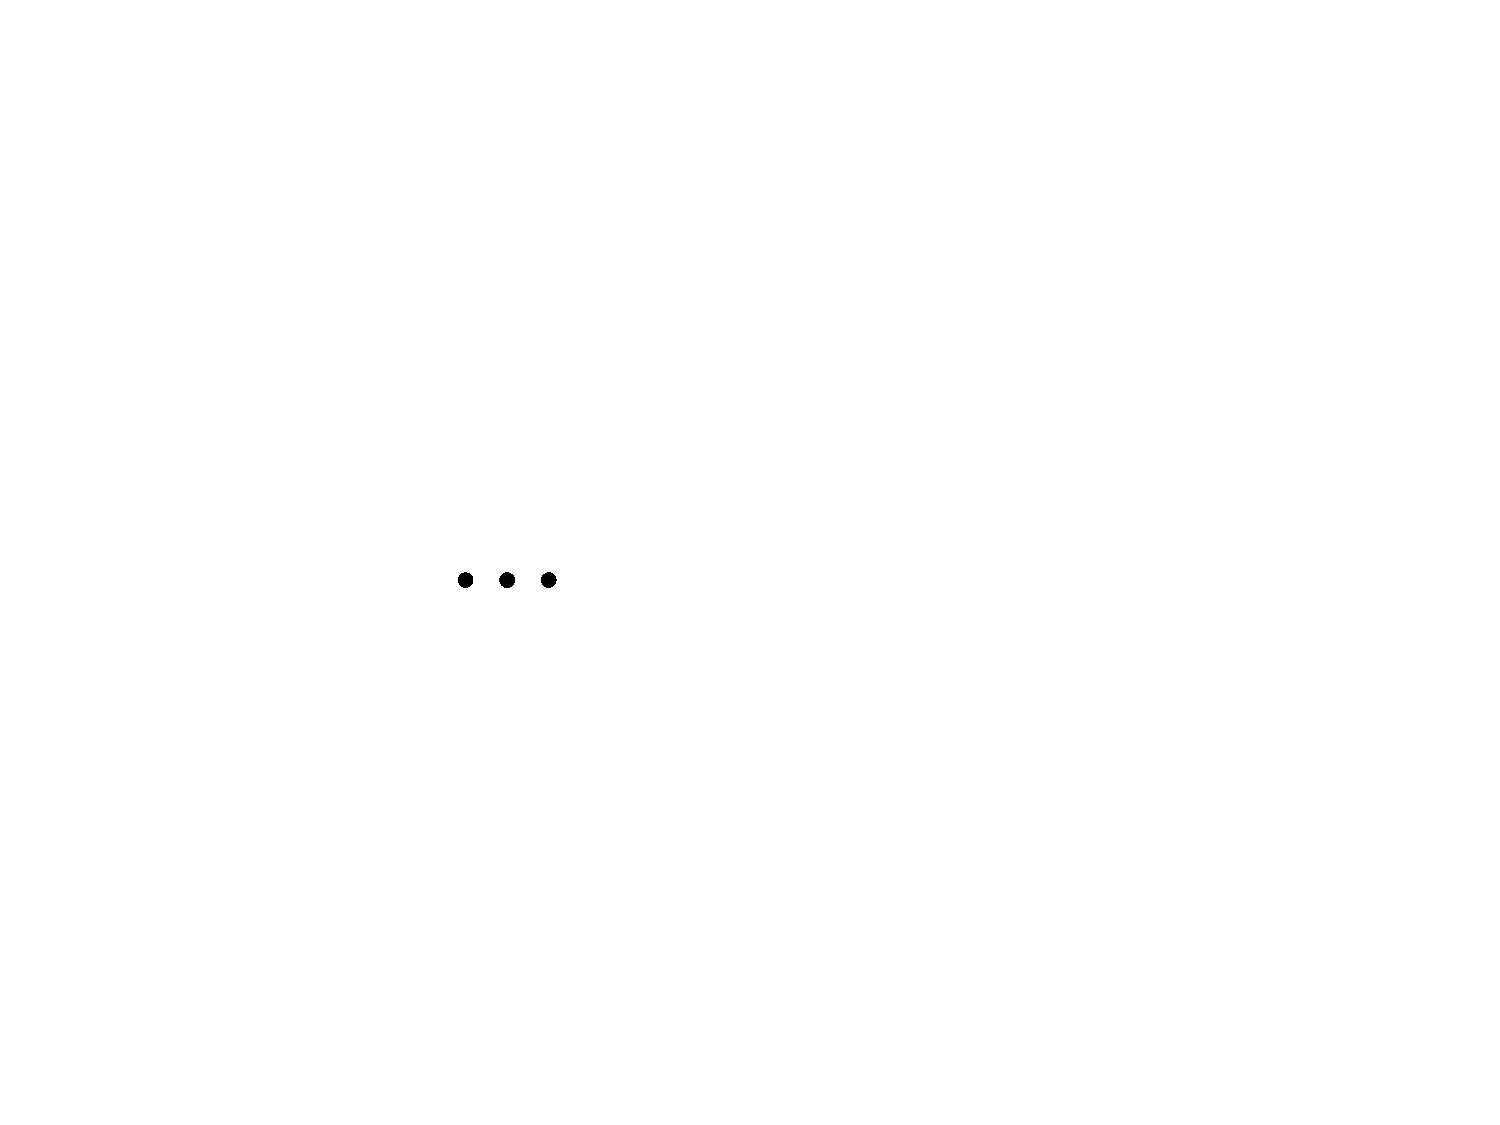
\includegraphics[width=0.7cm]{dots2}
      \end{subfigure}
      \hspace{-0.8cm}
      \begin{subfigure}[b]{0.24\textwidth}
      \captionsetup{justification=centering}
      		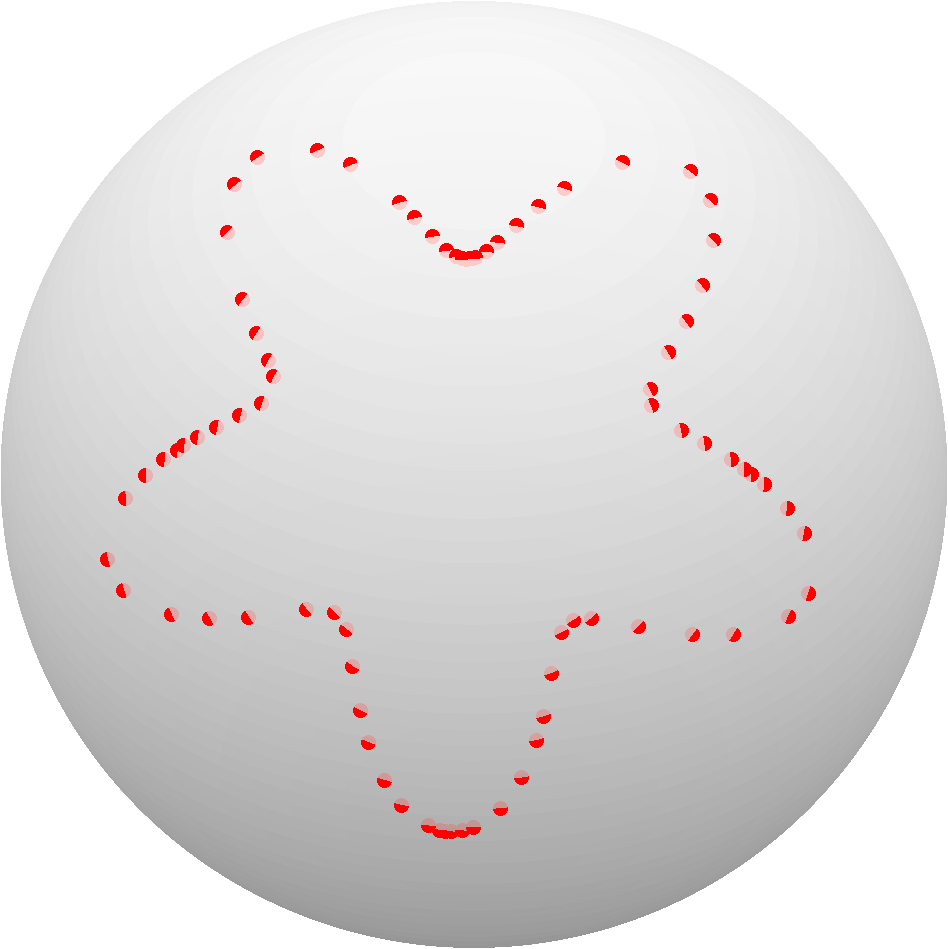
\includegraphics[width=\textwidth]{BFRecLev2SkelAll}
    		\caption{Skeleton points for $\Gamma_4$, ..., $\Gamma_{7}$.} 
        \end{subfigure}
    	\caption{Skeleton points on level 2 for the second and third off-diagonal row blocks corresponding to $\Gamma_5$ and $\Gamma_{6}$ are shown in red. The black points correspond to skeleton points selected on level 1. After compressing all off-diagonal row blocks we obtain (c), which plots the skeleton points for $\Gamma_4$, ..., $\Gamma_{7}$. }
     	\label{fig: BFRecLev2Skeleton}
\end{figure}

Once these skeleton points have been obtained, we can write out the factorization for level 2: 
\begin{center}
	\begin{tabular}[b]{ccccccc}
$\underset{ \ 4n_2 \times 4n_2}{S^{(1)}}$ & $\approx$ & $ \underset{ \ 4n_2 \times 4k_2 \ }{U^{(2)}}$  &  $\underset{ \ 4k_2 \times 4k_2 \ } {S^{(2)}}$ & $\underset{ \ 4k_2 \times 4n_2 \ } {{(V^{(2)})}^*}$& + &$\underset{ \ 4n_2 \times 4n_2 \ }{D^{(2)}}$. \\ [.4cm]
	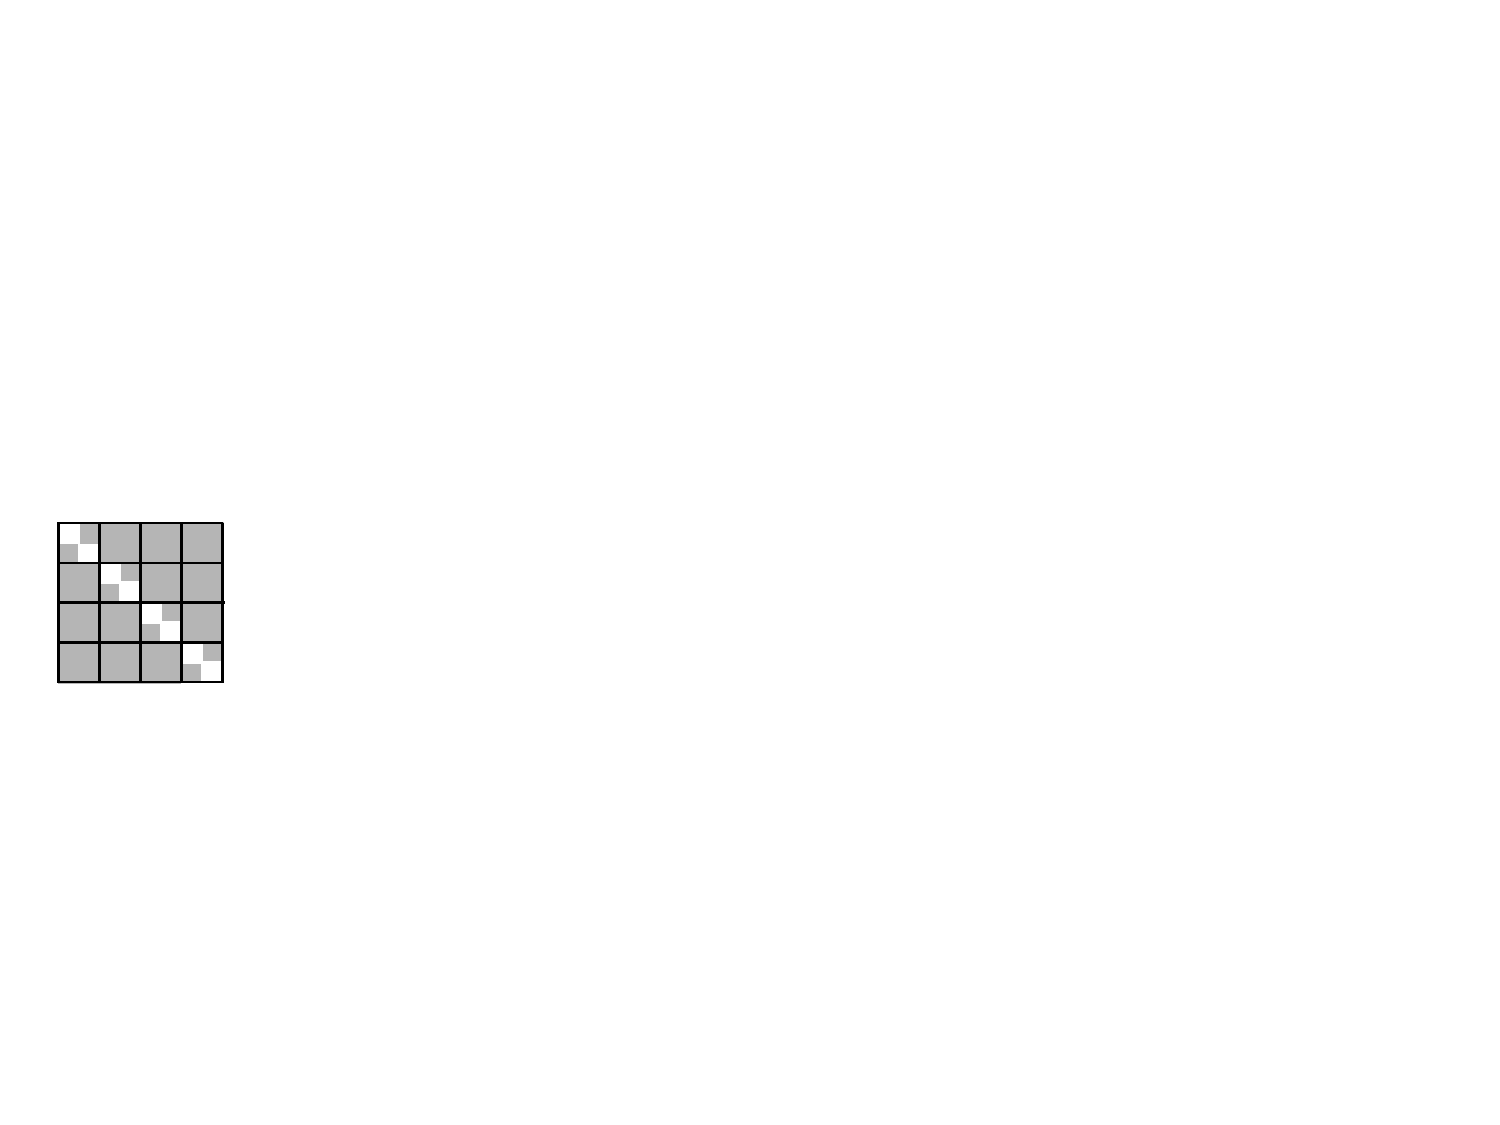
\includegraphics[width=1.68cm]{BFRecLev2S1} & & 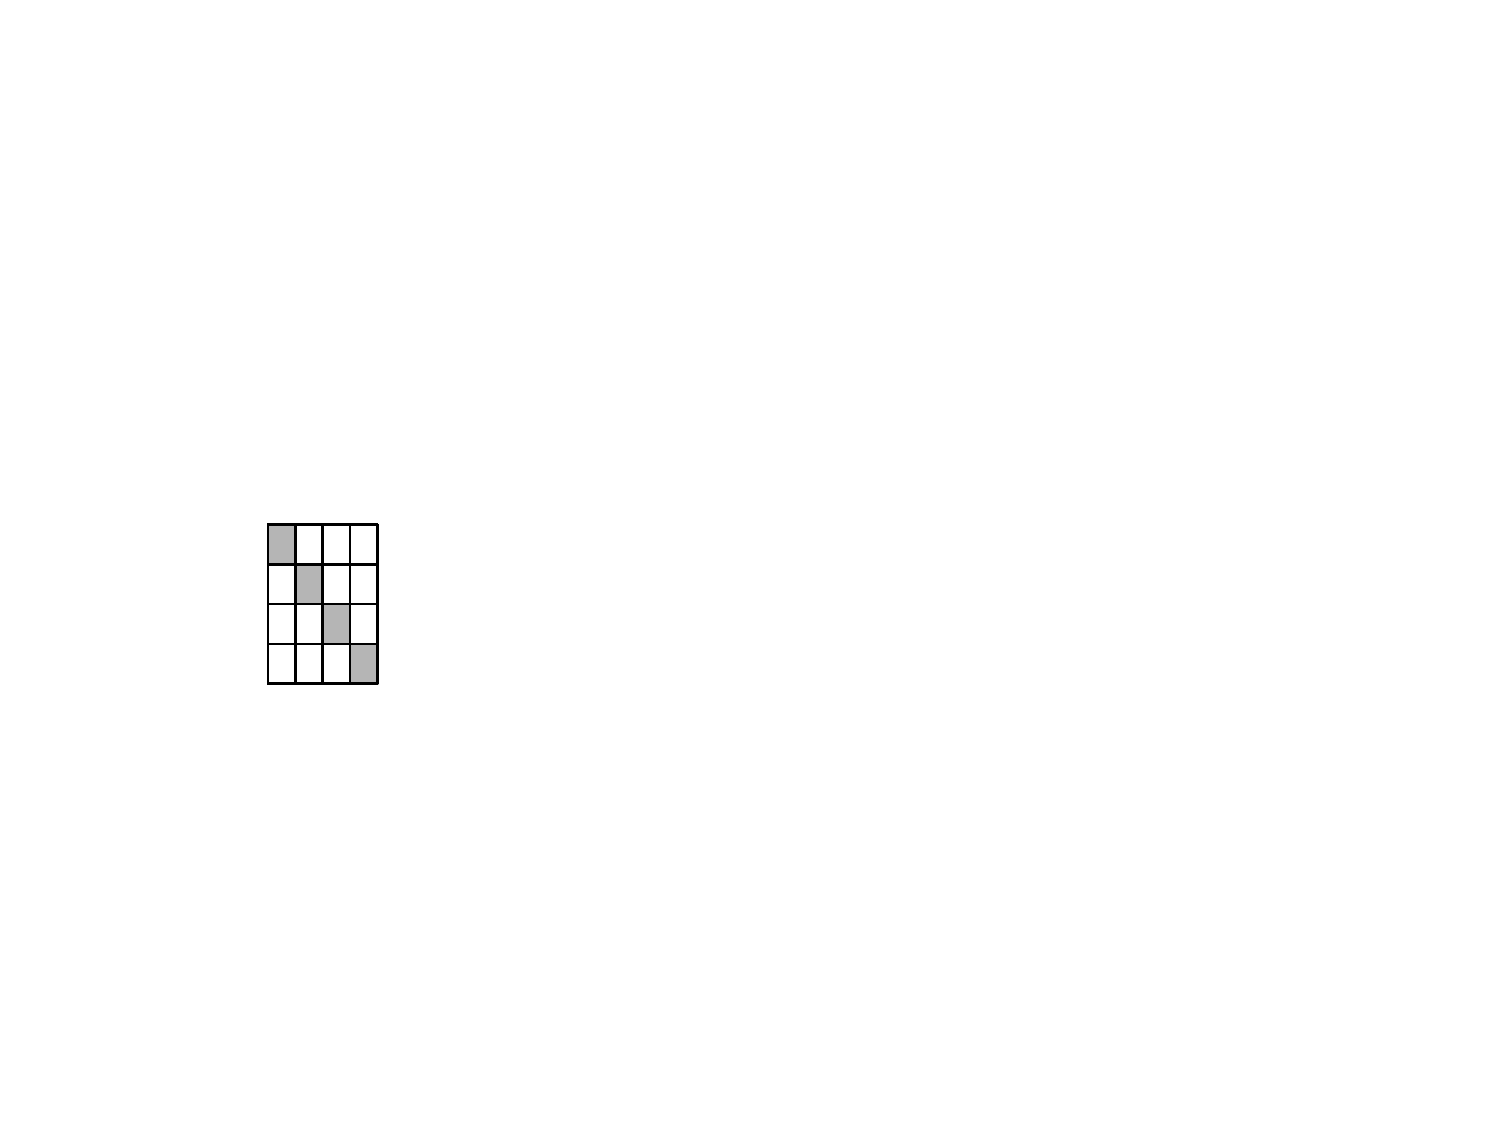
\includegraphics[width=1.15cm]{BFRecLev2U2} & 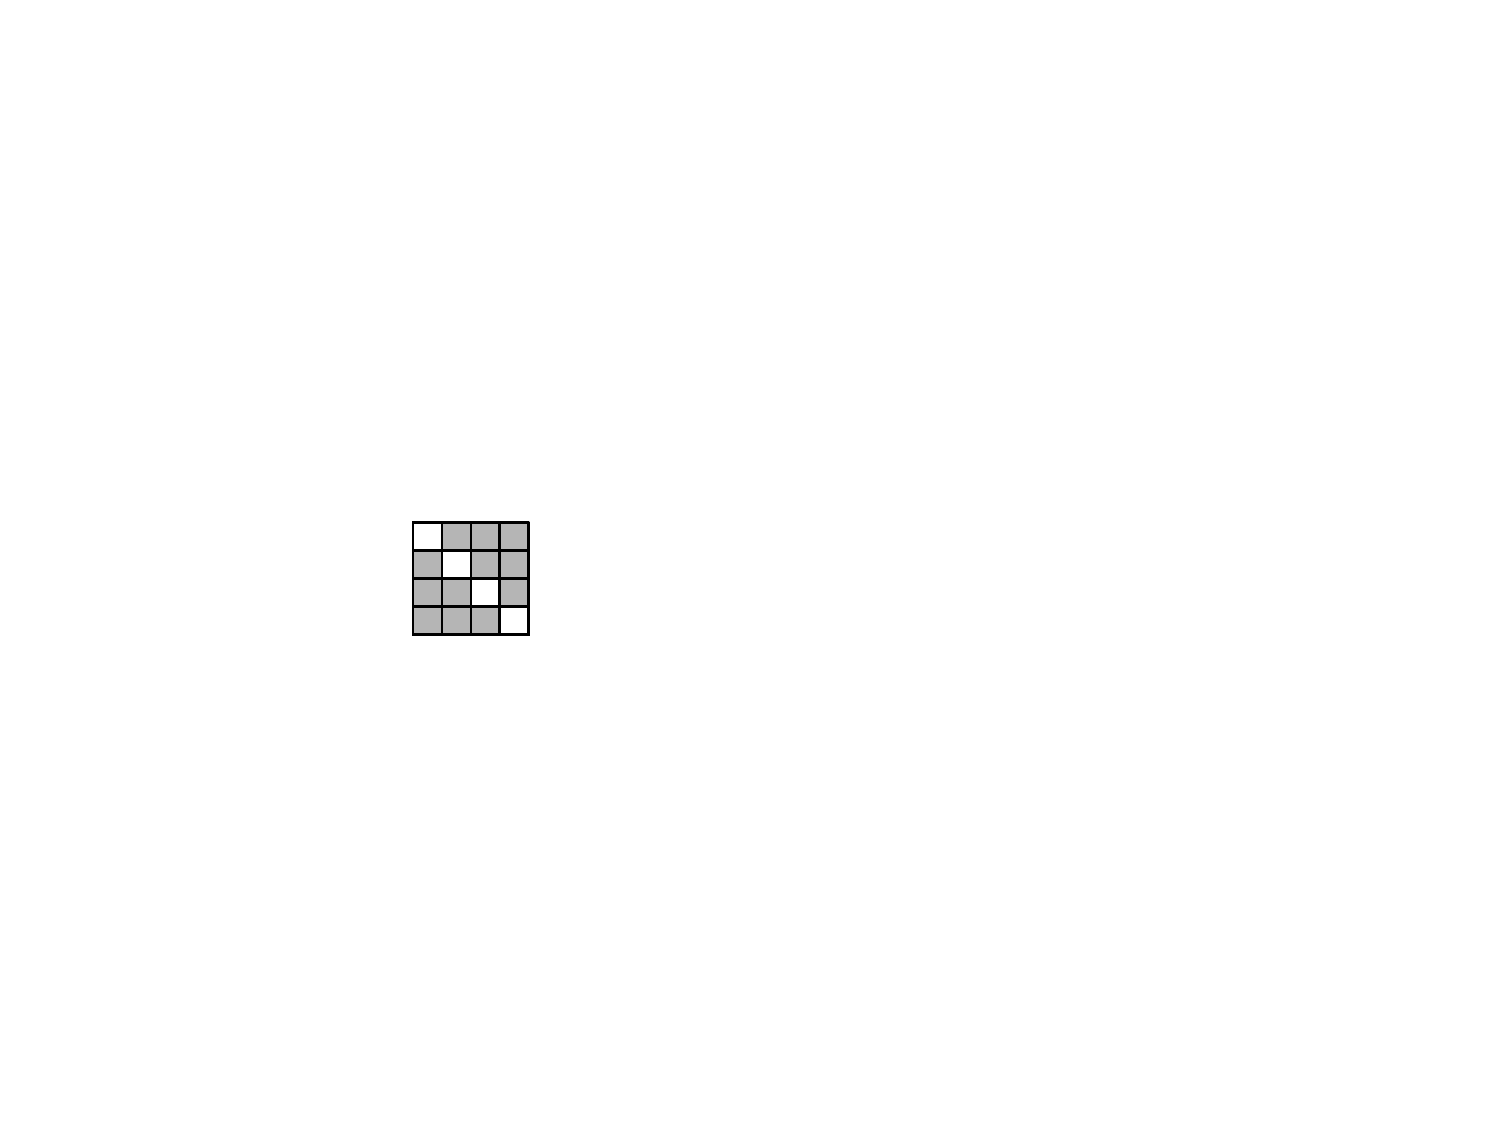
\includegraphics[width=1.2cm]{BFRecLev2S2} &\vspace{0.2cm}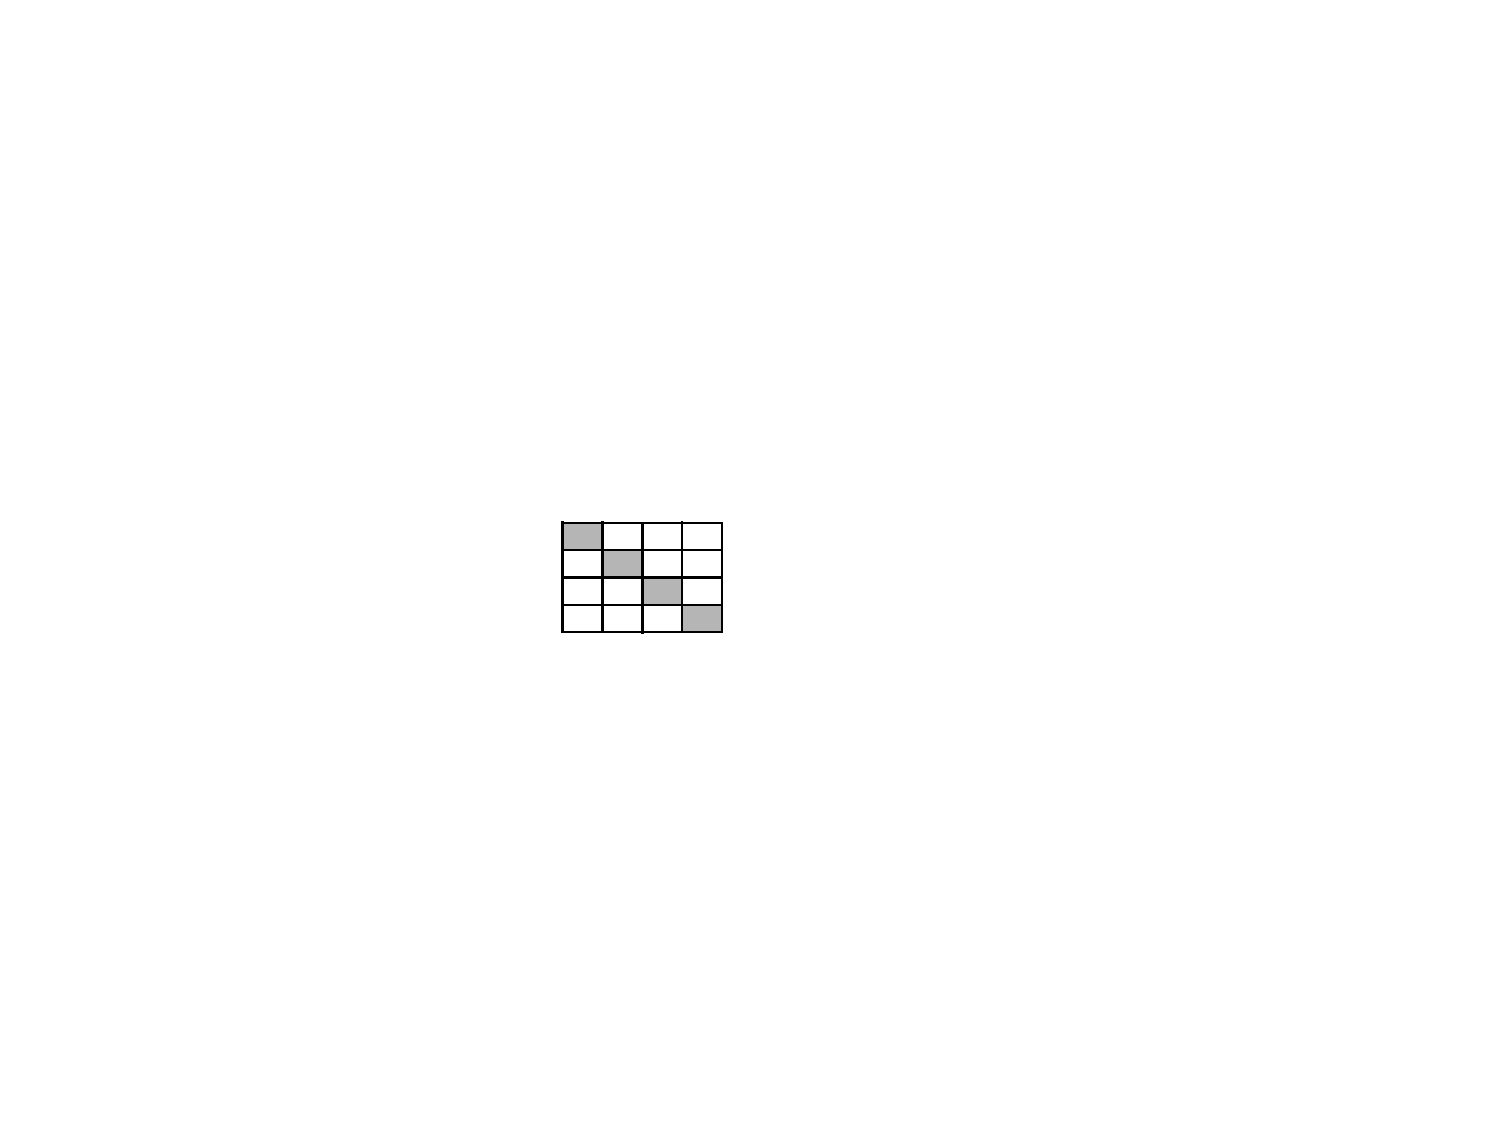
\includegraphics[width=1.68cm]{BFRecLev2V2} &  &  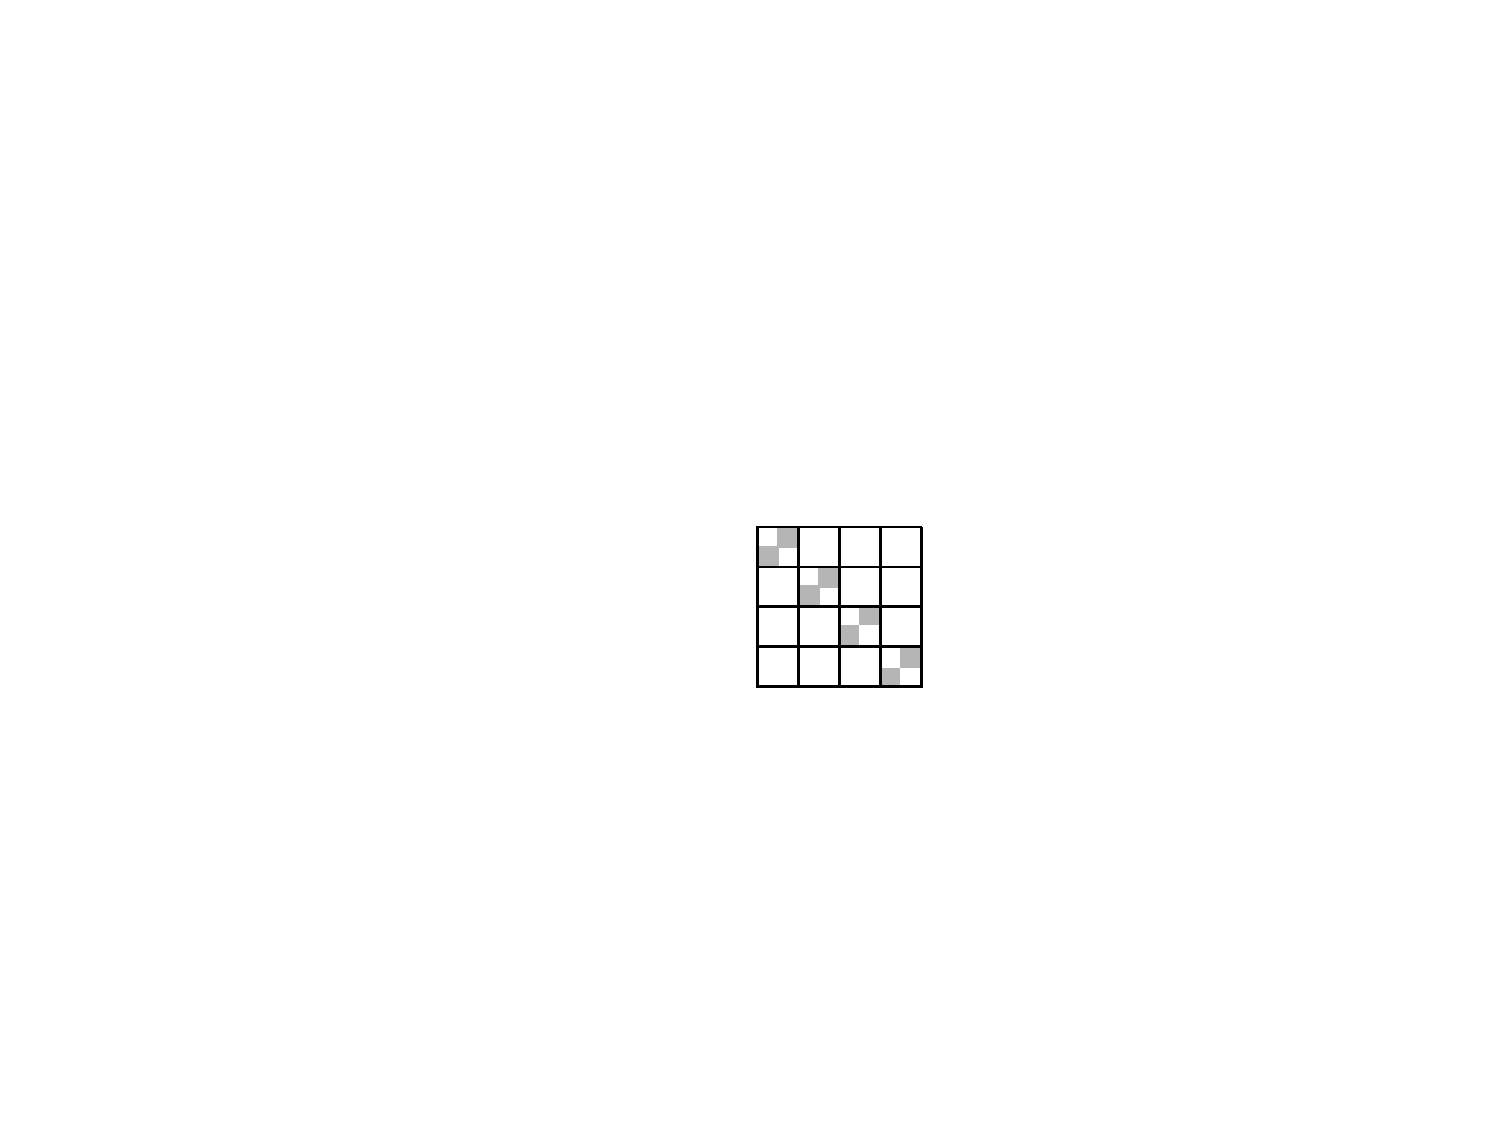
\includegraphics[width=1.68cm]{BFRecLev2D2} 
	\end{tabular}
\end{center}

%--------------------------------------------------------------------------------------------------------------------------------------------------------------------------------------------------------------------------------------

\subsubsection{Level 3}
The recursive algorithm continues until the compressed matrix $S^{(l)}$ on level $l=\lambda$ is a $2 \times 2$ block matrix. In this example applying one more level of recursion gives a $2\times2$ block matrix, $S^{(3)}$. On level 3 we set $n_3=2k_2$ and $p_3=2$. Compressing the two horizontal and vertical off-diagonal blocks gives the skeletons shown in Figure \ref{fig: BFRecLev3Skeleton}. 
\begin{figure}[h]
	\centering
	\begin{subfigure}[b]{0.24\textwidth}
	\captionsetup{justification=centering}
		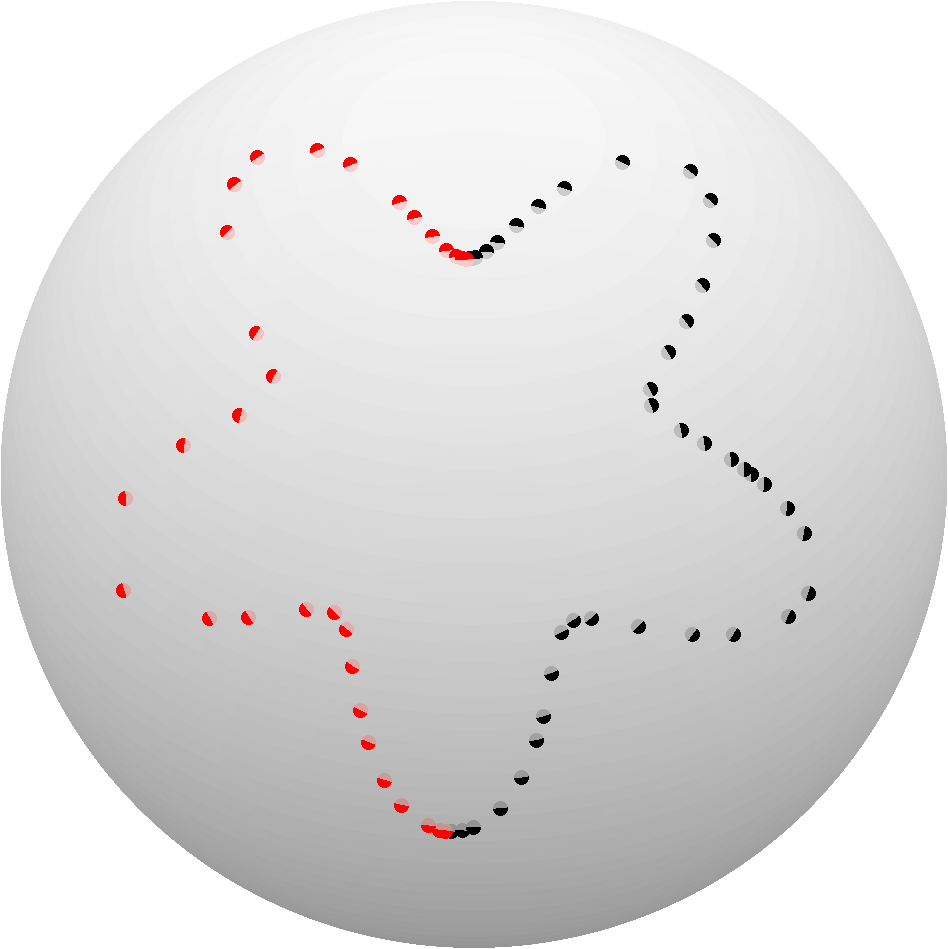
\includegraphics[width=\textwidth]{BFRecLev3Skel2}
    		\caption{Skeleton points for $\Gamma_2$.} 
      \end{subfigure}
      \quad
      \begin{subfigure}[b]{0.24\textwidth}
      \captionsetup{justification=centering}
      		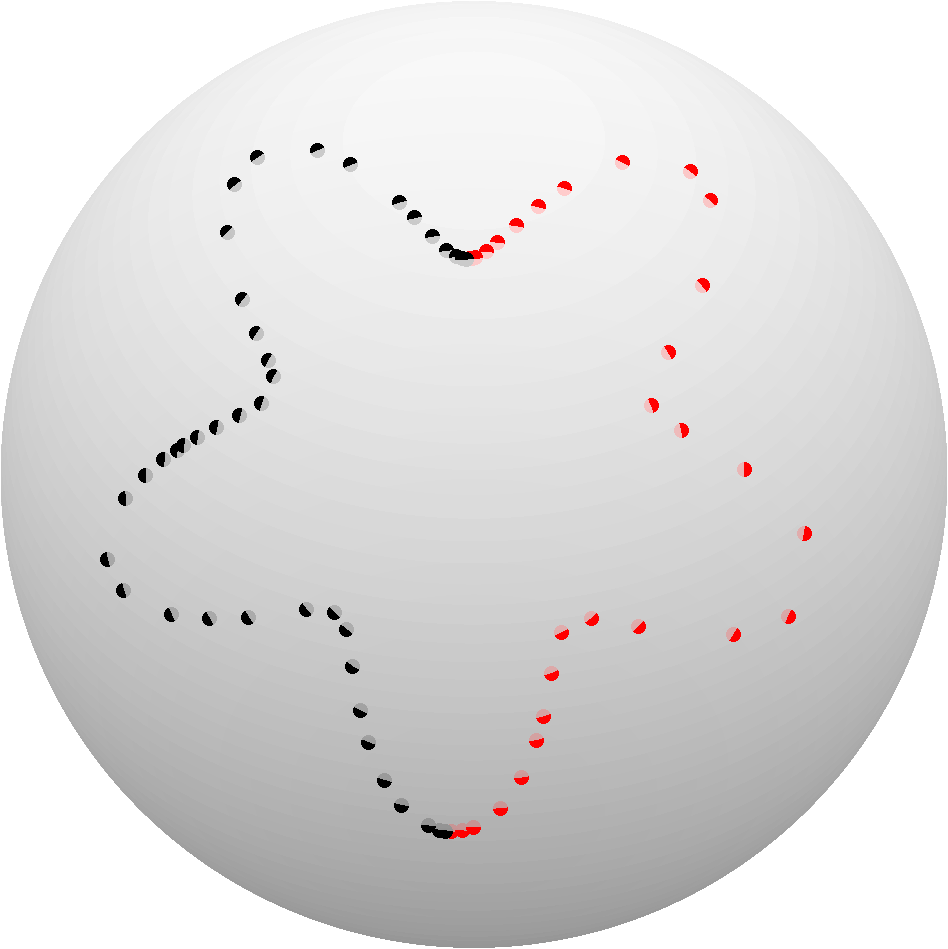
\includegraphics[width=\textwidth]{BFRecLev3Skel3}
    		\caption{Skeleton points for $\Gamma_{3}$.} 
       \end{subfigure}
       \quad
      \begin{subfigure}[b]{0.24\textwidth}
      \captionsetup{justification=centering}
     	 	\includegraphics[width=\textwidth]{BFRecLev3SkelAll}
    		\caption{Skeleton points for $\Gamma_2$ and $\Gamma_{3}$.} 
    		\label{fig: BFRecLev3SkelAll}
    \end{subfigure}
    \caption{Skeleton points on Level 3 for the two off-diagonal row and column blocks corresponding to $\Gamma_2$ and $\Gamma_{3}$ are shown in red. The final number of skeleton points in (c) is $2k_3=61$}
    \label{fig: BFRecLev3Skeleton}
\end{figure}

The resulting factorization for $S^{(2)}$ is
\begin{center}
	\begin{tabular}[b]{ccccccc}
$\underset{2n_3 \times 2n_3}{S^{(2)}}$ & $\approx$ & $ \underset{ \ 2n_3 \times 2k_3 \ } {U^{(3)}}$  &  $\underset{ \ 2k_3 \times 2k_3 \ }{S^{(3)}} $ & $\underset{ \ 2k_3 \times 2n_3 \ }{{(V^{(3)})}^*}$& + &$\underset{2n_3 \times 2n_3}{D^{(3)}}.$ \\ [.4cm]
	\includegraphics[width=1.2cm]{BFRecLev3S2} & & \includegraphics[width=0.7cm]{BFRecLev3U3} & \includegraphics[width=0.7cm]{BFRecLev3S3} &\vspace{0.2cm}\includegraphics[width=1.2cm]{BFRecLev3V3} &  &  \includegraphics[width=1.2cm]{BFRecLev3D3} 
	\end{tabular}
\end{center}

Comparing the original contour in Figure \ref{fig: OffDiagExContour}, with Figure \ref{fig: BFRecLev3SkelAll}, the "skeletonization" feature of fast direct solvers becomes very evident. Level by level we identify the columns and rows of $A$ which form a basis for its off-diagonal blocks, to some preset precision. The resulting factorization then expresses $A$ in terms of linear combinations of these rows and columns. Starting with $N=400$, the recursive compression algorithm reduces the number of points needed to discretize $\Gamma$ to $2k_3=61$ on level 3, with a level of precision of $\varepsilon=10^{-5}$. We can observe that these skeleton points tend to cluster at the points where $\Gamma$ is divided on each level (Figure \ref{fig: BFRecLev3SkelAll}).
Building the recursive levels back up we obtain the following factorization for A:
\begin{align}
\tabcolsep=0.05cm
	\begin{tabular}[t]{ccccccccccccccc}
	$A$ & $\approx$ & $U^{(1)} $  &  $(U^{(2)} $ & $(U^{(3)}$ & $S^{(3)}$ & ${(V^{(3)})}^*$ & + & $D^{(3)})$ & ${(V^{(2)})}^*$ &+ & $D^{(2)})$ & ${(V^{(1)})}^* $& + & $D^{(1)}.$ \\ [.4cm] 
& & \includegraphics[width=1.02cm]{BFRecLev1U1} & \includegraphics[width=0.74cm]{TelBFRecLev2U2} &  \includegraphics[width=0.45cm]{TelBFRecLev3U3} & \includegraphics[width=0.45cm]{TelBFRecLev3S3} & \includegraphics[width=0.73cm]{TelBFRecLev3V3} & &\includegraphics[width=0.75cm]{TelBFRecLev3D3}& \includegraphics[width=1.04cm]{TelBFRecLev2V2} & & \includegraphics[width=1.04cm]{TelBFRecLev2D2} & \includegraphics[width=1.83cm]{TelBFRecLev1V1}& & \includegraphics[width=1.9cm]{BFRecLev1D1}
	\end{tabular}
	\label{eq: BFRecTelescopeFact}
\end{align}

We note that all the factors in (\ref{eq: BFRecTelescopeFact}), except for $S^{(3)}$, are block diagonal matrices which can be efficiently built and processed. Thanks to the sparsification of rows and columns the matrix $S^{(3)}$ has much smaller dimension than $A$ and can be easily inverted. Applying the Sherman-Morrison-Woodbury formula from Section \ref{sec: SingLevel} recursively to this telescoping factorization, also gives a telescoping representation for $A^{-1}$ \cite{GillYoungMart2012}. Again, we omit the details for now and address inversion in more detail in Section \ref{sec: umfpack}. The advantage of the formula is that it preserves the nice structure in the telescoping blocks, so $A^{-1}$ is also represented in terms of block diagonal factors, and a smaller compressed matrix \cite{GillYoungMart2012}.  This ensures that $A^{-1}$ can be cheaply applied to any right hand side.

\subsubsection{Cost of Recursive Brute Force Compression and Inversion}
The recursive cost of compression is determined from the cost of repeatedly applying the ID on each level. In \cite{MartRokh2005} Martinsson and Rokhlin give a detailed breakdown of the complexity analysis showing that the total cost of obtaining the telescoping factorization (\ref{eq: BFRecTelescopeFact}) is $O(n_1N^2)$. 

When this recursive skeletonization procedure is used as-is, it is referred to as the \enquote{brute force} method. It can be applied to any matrix with structured rank-deficient off-diagonal blocks. Matrices of this type, which admit a telescoping factorization such as (\ref{eq: BFRecTelescopeFact}), are referred to as \textit{hierarchically block separable} \cite{GillYoungMart2012}. 

Since the $O(N^2)$ cost is determined from the cost of repeatedly applying the ID/pivoted QR, the only way to reduce the overall brute force cost is to reduce the dimension of the horizontal and vertical off-diagonal blocks being compressed. In order to do this the solver utilizes the physical interpretation of the ID and its connection with the double layer potential of the Laplace-Beltrami operator. More generally, direct solvers relate the ID with the underlying potential in a BIE operator, which is associated with Green's theorems for the underlying PDE \cite{HoGreen2012, MartRokh2005, GillYoungMart2012}.

We also note that for the recursive procedure the cost of inverting the telescoping factorization (\ref{eq: BFRecTelescopeFact}) drops to $O(N)$ \cite{MartRokh2005}. Thus once the compression stage is accelerated to $O(N)$ the overall cost of the solving the system will drop to $O(N)$ overall. 

% SECTION 3.5 --------------------------------------------------------------------------------------------------------------------------------------------------------------------------------------------

\section{Accelerating Compression: Proxy Points in 2D} 
\label{sec: 2DProxy}
The main factor driving the time complexity of the brute force method is the large dimension of the off-diagonal blocks that need to be compressed with pivoted QR on each level (blocks (\ref{eq: BFRecLev1HorBlock8} ), and (\ref{eq: BFRecLev2HorBlock4}) for example). Taking level 1 as an example, if the matrix $A$ is decomposed into $p \times p$ blocks of size $n$, then $A(I_\tau, L_\tau)$ has dimension $n \times (p-1)n$  (the subscripts on $p$ and $n$ are dropped for clarity). This gives a cost of $O(kn^2(p-1))$ for the ID. To reduce the cost of compressing such a block, we want to reduce its dimension without changing its range. 

For Laplace's equation, fast direct solvers accelerate the brute force method in 2D and 3D by exploiting the fact that the system matrix associated with a discretized BIE corresponds to evaluating a potential field. The rank-deficient off-diagonal blocks can then be interpreted as representing far field interactions between clusters of points. This implies that charges lying in the far field can be approximated with a smaller set of points. 

For the Laplace-Beltrami equation, we recall from Section \ref{sec: BIEFormulation} that the BIE is given by (\ref{eq: LB_BIE}), which is derived from the double layer potential on the sphere (\ref{eq: DLP}). 
We recall from Section \ref{sec: StereographicProjection} that after applying the stereographic mapping (\ref{eq: Sphere2Stereo}), (\ref{eq: LB_BIE}) can be equivalently represented in the stereographic $\xi$ plane by 
\begin{align}
	\frac{1}{2}\sigma(\xi)+\text{Re}\left\{\frac{1}{2\pi i}\int_{\tilde{\Gamma}} \sigma(\xi ')\left[\frac{1}{\xi -\xi '} - \frac{\bar{\xi} ' }{1+ {|\xi '|}^2}\right] d\xi ' \right\}= g(\mathbf{x}(\xi)). 
	\label{eq: BIEStereo}
\end{align}
We note that the first term in the kernel (\ref{eq: BIEStereo}) is the double layer potential for Laplace's equation in the plane. 
The single-layer potential in the stereographic plane also has a similar form to the one in the 2D plane, except that the density has to satisfy an extra constraint, as discussed in Section \ref{sec: BIEFormulation}. 

Due to the similarity between the kernels in the stereographic and 2D plane, we first examine the acceleration scheme for Laplace's equation in 2D. 
The scheme is extended to the sphere in the next section, and later the brute force example from Section \ref{sec: BFRecCompression} is repeated with proxy points to show how the acceleration scheme works in practice. 

% SECTION 3.5.1 -------------------------------------------------------------------------------------------------------------------------------------------------------------------------------------------

\subsection{Relationship to Potential Theory}
For simplicity we follow previous work in \cite{MartRokh2005, GillYoungMart2012, HoGreen2012} and start by explaining the acceleration process for a matrix associated with the discretized single-layer potential. The $\tau^{th}$ horizontal off-diagonal block is then associated with the operator,
\begin{align}
	K(\mathbf{x}, \mathbf{x}')\sigma(\mathbf{x}')=\int_{\Gamma_\tau^c} \sigma(\mathbf{x}') \log|\mathbf{x}-\mathbf{x}'|ds', \quad \mathbf{x}\in \Gamma_\tau, \label{eq: 2DPotentialGammaTau} 
\end{align}
where the boundary $\Gamma$ is divided into two parts: $\Gamma_\tau$ and $\Gamma_\tau^c$, corresponding to $I_\tau$ and $L_\tau$ (Figure \ref{fig: 2DGammaTauGammaTauC}).

\begin{figure}
	\centering
    	\includegraphics[width=0.4\textwidth]{2DGammaTauGammaTauC}
    	\caption{An example of a boundary contour corresponding to equation (\ref{eq: 2DPotentialGammaTau}). $\Gamma$ is divided into two parts: $\Gamma_\tau$ and $\Gamma_\tau^c$. }
    	\label{fig: 2DGammaTauGammaTauC}
\end{figure}

Physically, $\log|\mathbf{x}-\mathbf{x}'|$ represents the potential at $\mathbf{x}$ due to a point source located at $\mathbf{x}'$. The integral (\ref{eq: 2DPotentialGammaTau}) then represents the potential on $\Gamma_\tau$ due to a continuous charge distribution on $\Gamma_\tau^c$ with charge density $\sigma(\mathbf{x}')$. 

$\Gamma_\tau^c$ can be further broken down into two sections: $\Gamma_{\text{near}}$ and $\Gamma_{\text{far}}$, representing sources in the near and far field respectively. Thus $K(\mathbf{x}, \mathbf{x}')\sigma(\mathbf{x}')$ can be written as, 
\begin{align*}
	K(\mathbf{x}, \mathbf{x}')\sigma(\mathbf{x}') = \int_{\Gamma_{\text{near}}} \sigma(\mathbf{x}') \log|\mathbf{x}-\mathbf{x}'|ds' + \int_{\Gamma_{\text{far}}} \sigma(\mathbf{x}') \log|\mathbf{x}-\mathbf{x}'|ds', \quad \mathbf{x}\in \Gamma_\tau. 
\end{align*}
Similar to the FMM, the contributions of distant sources on $\Gamma_{\text{far}}$ decay rapidly. As a result they can be approximated by a smaller set of sources which lie on a new "artificial" contour $\Gamma_{\text{proxy}}$, shown in Figure \ref{fig: 2DGammaTauNearFarProxy}. 

\begin{figure}[h]
	\centering
	\includegraphics[width=0.4\textwidth]{2DGammaTauNearFarProxy}
	\caption{Sources on $\Gamma_\tau^c$ divided into two sets: $\Gamma_{\text{near}}$ and $\Gamma_{\text{far}}$. The new artificial contour, denoted by $\Gamma_{\text{proxy}}$, contains an equivalent density distribution representing the far field contributions. }
	\label{fig: 2DGammaTauNearFarProxy}
\end{figure}

More specifically, the charges on $\Gamma_{\text{far}}$ induce a harmonic field inside $\Gamma_{\text{proxy}}$ (Figure \ref{fig: 2DGammaTauFarProxy}). 
\begin{figure}[h]
 	\centering
    	\includegraphics[width=0.4\textwidth]{2DGammaTauFarProxy}
    	\caption{Sources on $\Gamma_{\text{far}}$ which induce a harmonic potential inside $\Gamma_{\text{proxy}}$.}
	\label{fig: 2DGammaTauFarProxy}
\end{figure}
The potential on $\Gamma_\tau$, given by 
\begin{align*}
	\int_{\Gamma_{\text{far}}} \sigma(\mathbf{x}') \log |\mathbf{x}-\mathbf{x}'| ds', \quad \mathbf{x}\in \Gamma_\tau, 
\end{align*}
is then harmonic and smooth inside $\Gamma_{\text{proxy}}$. Thus it can be equivalently represented by a charge distribution on $\Gamma_{\text{proxy}}$, 
\begin{align}
	\int_{\Gamma_{\text{proxy}}} \widetilde{\sigma}(\mathbf{x}') \log |\mathbf{x}-\mathbf{x}'| ds' = \int_{\Gamma_{\text{far}}} \sigma(\mathbf{x}') \log |\mathbf{x}-\mathbf{x}'| ds',  \quad \mathbf{x}\in \Gamma_\tau \label{eq: 2DPotentialProxy}. 
\end{align}

In the literature, the size of $\Gamma_{\text{proxy}}$ is determined by first surrounding $\Gamma_\tau$ by a circle of radius $r$. The radius of the proxy circle is then taken to be $1.5$ times larger, $r^{(\text{proxy})}=1.5r$. Correspondingly, $\Gamma_\text{near}$ and $\Gamma_\text{far}$ are the sections of $\Gamma_\tau^c$ which lie inside and outside $\Gamma_{\text{proxy}}$.

Similar steps can be applied to the vertical off-diagonal blocks. The $\tau^{th}$ vertical block is associated with the discretized operator 
\begin{align}
	K(\mathbf{x}, \mathbf{x}')\sigma(\mathbf{x}')=\int_{\Gamma_\tau} \sigma(\mathbf{x}') \log|\mathbf{x}-\mathbf{x}'|ds', \quad \mathbf{x}\in \Gamma_\tau^c. \label{eq: 2DPotentialGammaTauC} 
\end{align}
(\ref{eq: 2DPotentialGammaTauC}) now represents the potential on $\Gamma_\tau^c$ due to sources on $\Gamma_\tau$. We can think of this in terms of the exterior problem, where sources on $\Gamma_\tau$ generate a harmonic field outside of $\Gamma_{\text{proxy}}$. Ho and Greengard \cite{HoGreen2012} note that if the sources correctly evaluate the potential on $\Gamma_{\text{proxy}}$, then they can also reproduce the potential on $\Gamma_{\text{far}}$. 


% SECTION 3.5.2 -------------------------------------------------------------------------------------------------------------------------------------------------------------------------------------------

\subsection{Implementation}
\label{sec: 2DProxyImplementation}
Since we are dealing with the discretized form of these equations we only need to capture the charge distribution on $\Gamma_{\text{proxy}}$ to finite precision. In addition, since the contributions from the charges in the far field decay, $\Gamma_{\text{proxy}}$ can be represented by a discrete set of points, and in particular we can use a constant number of points, $J$, across all levels.

For this section, let the matrix $A$ denote the discretized matrix associated with the single layer potential, and let $A_{\text{proxy}}^H$ denote the discretized sources on $\Gamma_{\text{proxy}}$ generating a potential on $\Gamma_\tau$ (\ref{eq: 2DPotentialProxy}), given by 
\begin{align*}
	A_{\text{proxy}}^H \equiv \log |\mathbf{x}_i - \mathbf{x}'_j|, \quad \mathbf{x}_i\in \Gamma_\tau, \quad \mathbf{x}'_j \in \Gamma_{\text{proxy}},
\end{align*} 
where $i\in I_\tau$ and $j \in \{1,...,J\}$. 
Consequently, instead of compressing the full $n\times(p-1)n$ horizontal off-diagonal block
\begin{align}
	A(I_\tau, L_\tau)= \raisebox{-0.3\height}{\includegraphics[width=4cm]{2DProxyHorBlockRed}} = \raisebox{-0.3\height}{\includegraphics[width=4cm]{2DProxyHorBlockBlackGrey}}, 
	\label{eq: 2DProxyHorBlock}
\end{align}
we now compress 
\begin{align}
	&\underset{n\times (n^{(\text{near})}+ J)}{\left[\begin{array}{cc} 
	A(I_\tau, L^{(\text{near})}_\tau)  &  A_{\text{proxy}}^H 
	\end{array} \right]}=\raisebox{-0.3\height}{\includegraphics[width=2cm]{2DProxyHorReducedBlock}}= U_\tau S_{\text{temp},}  \label{eq: 2DProxyHorReducedBlock} 
\end{align}
where $n^{(\text{near})}$ denotes the number of points on $\Gamma_{\text{near}}$ and $n^{(\text{near})}+ J << (p-1)n$. In (\ref{eq: 2DProxyHorBlock}), the colour red is used to denote row indices, or targets, while black and grey are used to denote the column indices corresponding to sources in the near and far field. The proxy sources approximating the far field are shown in green in (\ref{eq: 2DProxyHorReducedBlock}). 
The ID of the reduced block (\ref{eq: 2DProxyHorReducedBlock}) given by $U_\tau S_{\text{temp}}$, provides the indices of the $k$ rows of the reduced block which form a basis for the row space, and the linear combinations of these rows. This information can then be applied to the original off-diagonal block $A(I_\tau, L_\tau)$ to give 
\begin{align*}
	\begin{tabular}{ccc}
	$\underset{ n \times (p-1)n }{A(I_\tau, L_\tau)}$ &$\approx$ & $\underset{ \ n \times k \ }{U_\tau}\underset{ \ k \times (p-1)n \ }{S_{R_\tau}.}$\\
	\includegraphics[width=0.3\textwidth]{2DProxyHorBlockTau} & & \includegraphics[width=0.3\textwidth]{2DProxyHorSkelTau}
	\end{tabular}
\end{align*}
where $S_{R_\tau}$ contains the $k$ rows of $A(I_\tau, L_\tau)$ which form a basis for the row space, corresponding to the indices determined from the ID of the reduced block (\ref{eq: 2DProxyHorReducedBlock}). 

The compression of vertical blocks works the same way. If we define 
\begin{align*}
	A_{\text{proxy}}^V=\log |\mathbf{x}_i - \mathbf{x}'_j|, \quad \mathbf{x}_i \in \Gamma_{\text{proxy}}, \quad \mathbf{y}_j \in \Gamma_\tau,
\end{align*}
then each vertical off-diagonal block 
\begin{align}
	A(L_\tau, I_\tau)=\raisebox{-0.5\height}{\includegraphics[width=0.7cm]{2DProxyVerBlockBlue}} = \raisebox{-0.5\height}{\includegraphics[width=0.7cm]{2DProxyVerBlockBlackGrey}},  	\label{eq: 2DProxyVerBlock} 
\end{align}
can be compressed by applying the ID to the reduced block  
\begin{align}
	\underset{(n^{(\text{near})}+J)\times n}{\left[\begin{array}{c}
	A(L^{(\text{near})}_\tau, I_\tau)\\
	A_{\text{proxy}}^V
	\end{array} \right]} = \raisebox{-0.5\height}{\includegraphics[width=0.7cm]{2DProxyVerReducedBlock}}= S_{\text{temp}} V_{\tau}^*. \label{eq: 2DProxyVerReducedBlock} 
\end{align}
In (\ref{eq: 2DProxyVerBlock}) blue is used to denote the column indices, or sources, of the vertical block, while black and grey denote the targets in the near and far field. The new proxy targets are shown in green in (\ref{eq: 2DProxyVerReducedBlock}). 
Again, we can take the information from (\ref{eq: 2DProxyVerReducedBlock}) to obtain 
\begin{align*}
	\begin{tabular}{ccc}
	$\underset{ (p-1)n  \times n }{A(L_\tau, I_\tau)}$ &$\approx$ & $\underset{ \ (p-1)n \times k \ }{S_{C_\tau}}\underset{ \ k \times n \ }{V_{\tau}^*.}$\\
	\includegraphics[width=0.3\textwidth]{2DProxyVerBlockTau} & & \includegraphics[width=0.3\textwidth]{2DProxyVerSkelTau}
	\end{tabular}
\end{align*}
 
We note that, just as with the brute force algorithm, the row and column blocks can be compressed at the same time, so that $U=V$. 

The role of proxy points in the above compressions is to accelerate the process of identifying the $k$ skeleton points which lie on the original boundary $\Gamma$, denoting either source or target locations. As such, the reduced off-diagonal blocks, and the matrices $S_{\text{temp}}$, are only constructed temporarily. The final skeleton matrices $S_{R_\tau}$ and $S_{C_\tau}$ are built  by evaluating the original kernel at the $k$ skeleton locations selected from the ID of the reduced blocks.  

The size of $\Gamma_{\text{proxy}}$ and its distance from $\Gamma_{\tau}$ is determined more or less heuristically. Setting $r^{(\text{proxy})}<1.5r$ implies there are fewer points in the near field, and a larger far field is being approximated. In order to maintain the desired level of accuracy, the number of points on $\Gamma_{\text{proxy}}$ would then need to be increased. Setting $r^{(\text{proxy})}>1.5r$ leads to a larger near field, which means that less of the far field is being approximated, leading to better accuracy. However, a larger near field also means less computational savings. 

The number of proxy points needed on $\Gamma_{\text{proxy}}$ is determined from the desired accuracy. Typically the number of proxy points used on each level of the recursive skeletonization is fixed. Using $J=50$ has been observed to give an accuracy on the order of $10^{-10}$ \cite{GillYoungMart2012}. 

The discussion of proxy points for the single layer potential can analogously be extended to the double layer potential in 2D, which is the closer analogy to the problem we are solving on the sphere. 

%--------------------------------------------------------------------------------------------------------------------------------------------------------------------------------------------------------------------------------------

\subsubsection{A Note About Complexity:}

We recall that the cost of applying the ID to an arbitrary block is $O(kn(p-1)n)$. Thus the time complexity depends on two factors: the rank of the block and its dimension. Proxy points reduce the cost of the ID by reducing the dimension of an off-diagonal block. The rank of an off-diagonal block is determined from the rank of interaction between $\Gamma_\tau$ and $\Gamma_\tau^c$. Ho and Greengard \cite{HoGreen2012} and Martinsson and Rokhlin \cite{MartRokh2005} explain that for many BIE matrices, especially those arising from Laplace's equation, the rank $k_l$ on each level $l$ depends logarithmically on the number of points in each block, i.e. $k_l \approx \log(n_l)$. Combining this observation with the reduced block size, and summing over all levels then results in $O(N)$ complexity, for compression, inversion and solution of the system. Details are given in \cite{HoGreen2012, MartRokh2005}. 

%--------------------------------------------------------------------------------------------------------------------------------------------------------------------------------------------------------------------------------------

\subsubsection{A Note About Accuracy:}

Although an error estimate is available for the ID, (\ref{eq: IDError}), tracking how the error accumulates over the single level and recursive compression schemes is difficult. Furthermore, if 
\begin{align}
	||A-A_{\varepsilon}||<O(\varepsilon), \label{eq: FDSCompressionError} 
\end{align}
it is not necessarily the case that 
	\[||A^{-1}-A_{\varepsilon}^{-1}||<O(\varepsilon).\] 
Also, the error $\varepsilon$ in (\ref{eq: FDSCompressionError}) does not necessarily match the accuracy set for the ID.
However, in practice we can empirically observe that the growth of errors across levels is mild. Often the tolerance level set for the ID matches the resulting order of accuracy in $A_{\varepsilon}$. 
If A is well-conditioned, $||A^{-1}-A_{\varepsilon}^{-1}||$ should also have the same order of accuracy as the compressed matrix. 
In \cite{HoGreen2012}, Ho and Greengard give some basic error estimates confirming these statements. Gillman et al. also use a method involving power iteration to estimate the error a posteriori \cite{GillYoungMart2012}. 

% SECTION 3.6 -------------------------------------------------------------------------------------------------------------------------------------------------------------------------------------------

\section{Proxy Points on the Sphere}
\label{sec: 3DProxy}
The main reason why proxy points can be applied to solve Laplace's equation in 2D is that a harmonic function can be represented as a single or double layer potential in which sources only need to be placed along the boundary of the domain. 
For a simply connected domain on the sphere, \cite{GemmNigStein2008} shows that a smooth solution $u \in \Omega$ satisfying the Dirichlet Laplace-Beltrami equation (\ref{eq: DirLapBelt}) can only be represented as a single layer potential, 
\begin{align*}
	u(\mathbf{x})=\int_{\Gamma}\rho(\mathbf{x}')\left(-\frac{1}{2\pi}\log||\mathbf{x}-{\mathbf{x}'}||+\frac{1}{4\pi}\log2\right)ds', 
\end{align*}
if the density satisfies the constraint 
\begin{align}
	\int_{\Gamma}\rho(\mathbf{x}')ds'=0. \label{eq: SLPConstraint}
\end{align}
This constraint is a result of the Gauss constraint discussed in Chapter \ref{two}. Consequently proxy points cannot be applied in a straightforward way, since any reconfiguration of sources must satisfy (\ref{eq: SLPConstraint}). 

The double layer potential, on the other hand, does satisfy the Laplace-Beltrami equation without any further constraints, so the solution $u$ is given by 
\begin{align}
	u(\mathbf{x})=\frac{1}{2\pi}\int_{\Gamma}\sigma(\mathbf{x'})\frac{\partial}{\partial n'}\log||\mathbf{x}-\mathbf{x'}|| ds', \quad x \in \Omega.  \label{eq: DLPSoln} 
\end{align}
This implies that the double layer potential on the sphere satisfies the conditions to apply proxy points. Since it has the same physical interpretation on the sphere as in 2D, the same arguments for the implementation of proxy points carry over from Section \ref{sec: 2DProxy}. 

However, the topology of the sphere does affect how proxy circles are constructed. We first need to define a distance measure between two points on the sphere. 
Since points on the sphere lie in $\mathbb{R}^3$, we can either use 3D Euclidean distance or geodesic distance. We opt for Euclidean distance for a couple of reasons. First, the double layer potential (\ref{eq: DLPSoln}) is posed in terms of Euclidean distance, which implies that distances between sources and targets are measured the same way. Secondly, the construction of proxy circles for the direct solver only needs to be approximate. As long as the points in the near field are captured accurately, the arrangement of proxy points for the far field is flexible. 

Just as in 2D, the $\tau^{th}$ horizontal off-diagonal block of the Laplace-Beltrami BIE matrix (\ref{eq: LBSystem}), corresponds to evaluating the potential on a segment of the boundary, $\Gamma_\tau$. To define a proxy circle surrounding $\Gamma_\tau$, we proceed in the following way. 
Let $\mathbf{x}_i$, $i=1,...,n$, denote the points lying on $\Gamma_\tau$. As in 2D, we want to surround these points by a circle of radius $r$. On the sphere, this translates to defining a spherical cap which contains all of the points $\mathbf{x}_i \in \Gamma_\tau$. We first define an approximate centre, $\mathbf{x}_c$ of the points $\mathbf{x}_i$, by either taking the midpoint of the endpoints, or the centre of mass of the points, i.e.
\begin{align*}
	\mathbf{x}_c=\frac{\mathbf{x}_1+\mathbf{x}_n}{2}, \quad  \text{or}  \quad  \mathbf{x}_c=\frac{1}{n}\sum_{i=1}^n \mathbf{x}_i.
\end{align*}
Then $\mathbf{x}_c$ is projected onto the sphere. Specifically, we convert $\mathbf{x}_c$ into spherical coordinates, and set the radial component equal to 1. 

We then measure the Euclidean distance between $\mathbf{x}_c$ and each $\mathbf{x}_i$, and define $d$ by the max distance, 
\begin{align*}
	d=\max_{i=1,...,n}{||\mathbf{x}_c-\mathbf{x}_i||}_2.
\end{align*}
This distance allows us to define a corresponding spherical cap with radius $r$ which surrounds $\Gamma_\tau$ and is oriented with $\mathbf{x}_c$ as the north pole (Figure \ref{fig: caps}). Given the distance $d$ and the height between the furthest point $\mathbf{x}_i$ and $\mathbf{x}_c$, $r$ is given by 
	\[r=\sqrt{d^2-h^2}.\]
The equation for the boundary of the cap surrounding $\Gamma_\tau$ is then  
\begin{align*}
	(r \cos t, r \sin t, \sqrt{1-r^2}) \quad or, \quad (\sin \theta_c \cos t, \sin \theta_c \sin t, \cos \theta_c), 
\end{align*}
where $\theta_c$ denotes the angle of elevation in spherical coordinates of the cap. 

\begin{figure}[h]
	\centering
  	\includegraphics[width=0.4\textwidth]{ProxyCircleSphere}
  	\caption{The process of constructing a proxy circle. First a spherical cap surrounding $\Gamma_\tau$ (not shown here) is defined, and then a second cap is constructed which is $1.5d$ away from $\mathbf{x}_c$ in Euclidean distance. The second cap represents $\Gamma_{\text{proxy}}$.}
  	\label{fig: caps}
\end{figure}

The corresponding proxy circle, $\Gamma_{\text{proxy}}$, is constructed by ensuring that it is a distance of $1.5d$ away from $\mathbf{x}_c$. In other words, if we let $\mathbf{x}'_j$, $j=1, .., J$ denote the points on $\Gamma_{\text{proxy}}$, then 
\begin{align*}
	{||\mathbf{x}_c-\mathbf{x}'_j||}_2=1.5d, \quad j=1,..,J.
\end{align*}
Any point on the sphere outside the proxy circle is then defined to lie on $\Gamma_{\text{far}}$. 
Given $\mathbf{x}_c$ and the distance $1.5d$, we can define a spherical cap for the proxy circle, by specifying its angle of elevation $\theta_c$.  Without loss of generality we assume $\mathbf{x}_c=(0,0,1)$. Given $\mathbf{x}_c$ and a point on $\Gamma_\text{proxy}$, $\mathbf{x}'_j=(\sin \theta_c \cos \phi, \sin \theta_c \sin \phi, \cos \theta_c)$, the distance between them needs to satisfy 
\begin{align*}
	{(1.5d)}^2=\sin^2 \theta_c (\cos^2 \phi+\sin^2 \phi)+{(1-\cos \theta_c)}^2.
\end{align*}
Solving for $\theta_c$ gives 
\begin{align*}
	\theta_c=\arccos \left(1-\frac{{(1.5d)}^2}{2} \right).
\end{align*}
Once the proxy circle is constructed, points are classified as lying in the near or far field depending if they lie above or below the cap. 

A complication arises if $1.5d$ exceeds the maximum possible Euclidean distance between two points on the sphere, which is 2. This leads to separating the construction of proxy points into two cases: 

\begin{itemize}
\item Case 1: $1.5d<2$ \\
If the distance between $\Gamma_{\text{proxy}}$ and $\mathbf{x}_c$ does not exceed 2, then everything proceeds normally. Once the near and far field points are classified, the compression of the system matrix proceeds just as in 2D. Some examples are shown in Figure \ref{fig: Case1}. 

\begin{figure}[h]
        \centering
        \begin{subfigure}[b]{0.4\textwidth}
                \includegraphics[width=\textwidth]{Case1ProxyEx1}
                \caption{Case 1 on finer level}
                       \end{subfigure}%
        ~ 
        \begin{subfigure}[b]{0.4\textwidth}
                \includegraphics[width=\textwidth]{Case1ProxyEx2}
                \caption{Case 1 on coarser level}
                     \end{subfigure}
        \caption{Case 1:  An example of proxy circles on the sphere where $1.5d<2$.}
        \label{fig: Case1}
  \end{figure}


\item Case 2: $1.5d\geq 2$\\
This case typically occurs on coarser levels when $\Gamma_\tau$ is larger. In this instance, no proxy circle is constructed, since the size of $1.5d$ indicates that the entire near field would need to be considered, and thus using a proxy circle would not provide any computational savings. Since this occurs on the coarser levels of the algorithm, $\Gamma$ is already quite sparse due to skeletonization, and so this step does not add to the computational cost. An example is shown in Figure \ref{fig: Case2}.  
\end{itemize}

\begin{figure}
	\centering
  	\includegraphics[width=0.4\textwidth]{Case2ProxyEx}
	 \caption{Case 2: An example of skeletonized points on the coarsest level of the algorithm. Since $1.5d\geq2$, no proxy circle is created.}
	 \label{fig: Case2}
\end{figure}
 
In Chapter \ref{four} we verify numerically that the recursive algorithm with proxy points on the sphere leads to the same $O(N)$ time complexity and similar accuracy as in the plane. 
%--------------------------------------------------------------------------------------------------------------------------------------------------------------------------------------------------------------------------------------

\subsubsection{Example}
We now refer back to the example shown in Section \ref{sec: BFRecCompression} for the brute force method. We repeat several steps to show how proxy points work in practice on the sphere. 
Again, the matrix $A$ represents the system matrix in (\ref{eq: LBSystem}) corresponding to the the discretized Laplace-Beltrami BIE (\ref{eq: LB_BIE}). 

Just as in Section \ref{sec: BFRecCompression}, $A$ is divided into $p_1=8 \times 8$ blocks, of size $n_1=50$, and we compress the matrix level by level based on the same binary tree (\ref{eq: BinaryTree}) used for the brute force method. 

The relative precision of the ID is still set to $\varepsilon=10^{-5}$ and the number of points on each proxy circle is set to $J=50$. 

%--------------------------------------------------------------------------------------------------------------------------------------------------------------------------------------------------------------------------------------

\subsubsection{Level 1}
We begin by compressing the first horizontal off-diagonal block, $A(I_8, L_8)$, shown in (\ref{eq: BFRecLev1HorBlock8}). 
To reduce its dimension we take $\Gamma_8$, surround it with a proxy circle, $\Gamma_{\text{proxy}}$, and divide $\Gamma_8^c$ into 2 parts: $\Gamma_{\text{far}}$ and $\Gamma_{\text{near}}$. Each of these segments is shown in Figure \ref{fig: ProxyRecLev1Block8}.
The index vector $L_8$ is similarly split into $L_8=L_8^{\text{(near)}} \cup L_8^{\text{(far)}}$.

$A(I_8, L_8^{\text{(far)}})$ is then discarded from the off-diagonal horizontal block and replaced with the value of the discretized kernel along $\Gamma_{\text{proxy}}$, defined as, 
\begin{align*}
	A_{\text{proxy}}^H=K(\mathbf{r}_i, \mathbf{x}'_j)=-\frac{(\mathbf{r}_i-\mathbf{x}'_j)}{{||\mathbf{r}_i-\mathbf{x}'_j||}_2^2}\cdot \mathbf{n}_j ds_j, \quad \begin{array}{cc} 
	\mathbf{r}_i \in \Gamma_8, &\mathbf{x}'_j \in \Gamma_{\text{proxy}}\\
	i \in I_8 &j \in \{1, ..., 50\}.
\end{array}
\end{align*}
Here, $\mathbf{n}_j$ denotes the outward normal vector to the proxy circle. 

We then construct the reduced horizontal off-diagonal block, 
\begin{align*}
	&HB_8=\underset{n_1 \times (n^{(near)}+J)}{\left[\begin{array}{cc}
	A(I_8, L_8^{\text{(near)}}) & A_{\text{proxy}}^H
	\end{array}\right]}.
\end{align*}

At the same time, we build the reduced vertical block:
\begin{align*}
	A_{\text{proxy}}^V=K(\mathbf{x}_i, \mathbf{r}'_j)=-\frac{(\mathbf{x}_i-\mathbf{r}'_j)}{{||\mathbf{x}_i-\mathbf{r}'_j||}_2^2}\cdot \mathbf{n}_j ds_j, \quad \begin{array}{cc} 
	\mathbf{x}_i \in \Gamma_{\text{proxy}}, &\mathbf{r}'_j \in \Gamma_8\\
	i \in \{1, ..., 50\}, &j \in I_8,
	\end{array}
\end{align*}
\begin{align*}
	VB_8=\underset{(n^{(near)}+J) \times n^{(near)} }{\left[\begin{array}{c}
	A(L_8^{\text{(near)}}, I_8)\\
	A_{\text{proxy}}^V
	\end{array}\right].}
\end{align*}

These reduced  horizontal and vertical blocks are then compressed with the ID giving 
\begin{align*}
	\underset{n_1 \times 2(n^{(near)}+J)}{\left[\begin{array}{cc}
	HB_8& VB_8^*
	\end{array}\right]}=\underset{ \ n_1 \times k_1 \ }{U_8} \underset{ \ k_1 \times 2(n^{(near)} +J) \ }{S_{\text{temp}}.}
\end{align*}
As noted in Section \ref{sec: 2DProxyImplementation}, $S_{\text{temp}}$ is not explicitly constructed. The indices of the $k_1$ skeleton points on $\Gamma_8$ (shown in Figure  \ref{fig: ProxyRecLev1Block8}), denoted by $\tilde{I}_8$, are used to select $k_1$ rows and columns of the original horizontal and vertical off-diagonal blocks. 
\begin{figure}[h]
	\centering
  	\includegraphics[width=0.4\textwidth]{ProxyRecLev1Block8}
 	\caption{Skeleton points on $\Gamma_8$ selected by the ID. The proxy circle, plotted in green, divides $\Gamma_8^c$ into $\Gamma_{\text{near}}$ and $\Gamma_{\text{far}}$, which are plotted in black and grey respectively. The $k_1$ skeleton points represent sources which induce a harmonic potential on $\Gamma_{\text{proxy}}$, or targets where the potential is evaluated due to sources on $\Gamma_{\text{proxy}}$. }
	\label{fig: ProxyRecLev1Block8}
\end{figure}

The factorizations for the original off-diagonal blocks are then given by
\begin{align*}
	A(I_8, L_8)&\approx U_8 A(\tilde{I}_8, L_8),\\
	A(L_8, I_8)&\approx A(L_8, \tilde{I}_8)U_8^* = A(L_8, \tilde{I}_8)V_8^*,
\end{align*}
where we assume $\tilde{I}_8$ takes into account the appropriate permutations applied to the rows and columns during the ID. 
The same procedure is carried out for the remaining 7 blocks on level 1. The resulting skeleton on $\Gamma$ is shown in Figure \ref{fig: ProxyRecLev1SkelAll}. 
\begin{figure}[h]
	\centering
	\includegraphics[width=0.3\textwidth]{ProxyRecLev1SkelAll}
	\caption{Skeleton points selected by the ID after one level of compression. }
	\label{fig: ProxyRecLev1SkelAll}
\end{figure}

$A$ is then factored just as in the brute force method to give 
\begin{align}
	& \underset{8n_1 \times 8n_1}{\hspace{1cm} A \hspace{1cm} }\approx \quad \underset{ \ 8n_1 \times 8k_1 \ }{U^{(1)}}  \underset{ \ 8k_1 \times 8k_1 \ }{S^{(1)}} \underset{ \ 8k_1 \times 8n_1 \ }{{(V^{(1)})}^*}+\underset{ \ 8n_1 \times 8n_1 \ }{D^{(1)}}. \label{eq: ProxyRecLev1Factorization} 
\end{align}
$S^{(1)}$ is comprised of the $8k_1$ rows and columns of the matrix $A$, corresponding to the indices of the skeleton points in Figure \ref{fig: ProxyRecLev1SkelAll}. 

%--------------------------------------------------------------------------------------------------------------------------------------------------------------------------------------------------------------------------------------

\subsubsection{Level 2}
Next, we set $p_2=4$, $n_2=2k_1$, and compress $S^{(1)}$ from (\ref{eq: ProxyRecLev1Factorization}). The index vectors $I_4$, $L_4$, for the first off-diagonal blocks are given by
\begin{align*}
	I_4&=\tilde{I}_8 \cup \tilde{I}_9\\
	L_4&=\tilde{I}_{10}, \cup ... \cup \tilde{I}_{15}.
\end{align*}
The first horizontal off-diagonal block is then denoted as $S^{(1)}(I_4, L_4)$, just as in (\ref{eq: BFRecLev2HorBlock4}). 
The same compression steps from level 1 are then repeated. 
A proxy circle $\Gamma_{\text{proxy}}$ is constructed around $\Gamma_4$ and the remaining points are split into $\Gamma_{\text{near}}$ and $\Gamma_{\text{far}}$ (Figure \ref{fig: ProxyRecLev2Block4}). 
The reduced horizontal and vertical blocks are then built: 
\begin{align*}
	S_{\text{proxy}}^H=K(\mathbf{r}_i, \mathbf{x}'_j), \quad \begin{array}{cc} 
	\mathbf{r}_i \in \Gamma_4, &\mathbf{x}'_j \in \Gamma_{\text{proxy}}\\
	i \in I_4 &j \in \{1, ..., 50\},
	\end{array}
\end{align*}
\begin{align*}
	S_{\text{proxy}}^V=K(\mathbf{x}_i, \mathbf{r}'_j), \quad \begin{array}{cc} 
	\mathbf{x}_i \in \Gamma_{\text{proxy}}, &\mathbf{r}'_j \in \Gamma_4\\
	i \in \{1, ..., 50\} &j \in I_4,
	\end{array}
\end{align*}
\begin{align*}
	HB_4=\left[\begin{array}{cc}
	S^{(1)}(I_4, L_4^{\text{(near)}}) & S_{\text{proxy}}^H
	\end{array}\right] \quad VB_4=\left[\begin{array}{c}
	S^{(1)}(L_4^{\text{(near)}}, I_4) \\ S_{\text{proxy}}^V
\end{array}\right].\\
\end{align*}

Applying the ID gives
\begin{align*}
	\underset{n_2 \times 2(n^{\text{(near)}}+J)}{\left[\begin{array}{cc}
	HB_4 & VB^*_4\end{array}\right]}=\underset{ \ n_2 \times k_2 \ }{U_4} \underset{ \ k_2 \times 2(n^{\text{(near)}}+J) \ }{S_{\text{temp}}.}
\end{align*}
The $k_2$ skeleton points selected are shown in Figure \ref{fig: ProxyRecLev2Block4}. 
\begin{figure}[h]
	\centering
  	\includegraphics[width=0.4\textwidth]{ProxyRecLev2Block4}
 	\caption{Skeleton points on $\Gamma_4$ selected by the ID. The proxy circle now surrounds skeletonized sources or targets from level 1. }
	\label{fig: ProxyRecLev2Block4}
\end{figure}

The factorizations for the first off-diagonal blocks are then 
\begin{align*}
	S^{(1)}(I_4, L_4)& \approx U_4S^{(1)}(\tilde{I}_4, L_4),\\
	S^{(1)}(L_4, I_4)& \approx S^{(1)}(L^4, \tilde{I}_4)U_4^*=S^{(1)}(L^4, \tilde{I}_4)V_4^*.
\end{align*}
Carrying out this same procedure on the remaining blocks we obtain the skeleton in Figure \ref{fig: ProxyRecLev2SkelAll}. 
\begin{figure}[h]
	\centering
	\includegraphics[width=0.3\textwidth]{ProxyRecLev2SkelAll}
	\caption{Skeleton points selected by the ID after two levels of compression. }
	\label{fig: ProxyRecLev2SkelAll}
\end{figure}
The resulting factorization for $S^{(1)}$, just as in Section \ref{sec: BFRecCompression}, is given by
\begin{align*}
	\underset{ \ 4n_2 \times 4n_2}{S^{(1)}} \approx \underset{ \ 4n_2 \times 4k_2 \ }{U^{(2)}}\underset{ \ 4k_2 \times 4k_2 \ } {S^{(2)}} \underset{ \ 4k_2 \times 4n_2 \ } {{(V^{(2)})}^*}+ \underset{4n_2 \times 4n_2}{D^{(2)}}.
\end{align*}
Again, $S^{(2)}$ is comprised of the $4k_2$ rows and columns of $S^{(1)}$ corresponding to the skeleton points in Figure \ref{fig: ProxyRecLev2SkelAll}.

%--------------------------------------------------------------------------------------------------------------------------------------------------------------------------------------------------------------------------------------

\subsubsection{Level 3}
On level 3 we have $p_3=2$, and $n_3=2k_2$. 
The indices of the first off-diagonal blocks are
\begin{align*}
	I_2=\tilde{I}_4 \cup \tilde{I}_5, \quad L_2=\tilde{I}_6 \cup \tilde{I}_7.
\end{align*}
$\Gamma_{\text{proxy}}$ is then constructed around $\Gamma_2$ (Figure \ref{fig: ProxyRecLev3Block2}). On this coarsest level we see that due to the size of $\Gamma_2$, the proxy circle surrounds the entire contour $\Gamma=\Gamma_2 \cup \Gamma_3$. Hence all of $\Gamma_2^c$ is included in the near field. This is common on coarser recursive levels for problems in 2D as well. However, the number of points on  $\Gamma_2^c$ is sparse from skeletonization on previous levels, so this does not have any noticeable effect on computation time or accuracy. 
\begin{figure}[h]
 	\centering
  	\includegraphics[width=0.4\textwidth]{ProxyRecLev3Block2}
 	\caption{Skeleton points on $\Gamma_2$ selected by the ID. The proxy circle surrounds skeletonized sources or targets from level 2. In this case, the entire section $\Gamma_2^c$ is considered in the near field. }
 	\label{fig: ProxyRecLev3Block2}
\end{figure}

The remainder of the algorithm proceeds normally. The reduced horizontal and vertical blocks are built
\begin{align*}
	HB_2=\left[\begin{array}{cc}
	S^{(1)}(I_2, L_2^{\text{(near)}}) & S_{\text{proxy}}^H
	\end{array}\right] \quad VB_2=\left[\begin{array}{c}
	S^{(1)}(L_2^{\text{(near)}}, I_2) \\ S_{\text{proxy}}^V
\end{array}\right], 
\end{align*}
and after compressing $\left[\begin{array}{cc} HB_2 & VB_2^* \end{array} \right]$, the corresponding skeleton points are shown in Figure \ref{fig: ProxyRecLev3Block2}.
The same steps are applied to obtain and compress  $\left[\begin{array}{cc} HB_3 & VB_3^* \end{array} \right]$.
The resulting skeleton for $\Gamma_2 \cup \Gamma_3$ is plotted in Figure \ref{fig: ProxyRecLev3SkelAll}.
\begin{figure}[h]
	\centering
	\includegraphics[width=0.3\textwidth]{ProxyRecLev3SkelAll}
	\caption{Skeleton points selected by the ID after three levels of compression}
	\label{fig: ProxyRecLev3SkelAll}
\end{figure}
Beginning with $N=400$, the number of skeleton points on $\Gamma$ after three levels of compression is $2k_3=75$, which is slightly higher than the 61 selected by the brute force method. Even though we obtain slightly higher ranks than the brute force approach, the reduced time complexity far outweighs the small growth in ranks.

Subsequently, the resulting factorization is 
\begin{align*}
	\underset{2n_3 \times 2n_3}{S^{(2)}} \approx \underset{ \ 2n_3 \times 2k_3 \ } {U^{(3)}}\underset{ \ 2k_3 \times 2k_3 \ }{S^{(3)}} \underset{\ 2k_3 \times 2n_3 \ }{{(V^{(3)})}^*}+\underset{ \ 2n_3 \times 2n_3 \ }{D^{(3)}}.
\end{align*}

Once the coarsest level is reached (i.e. level 3), the factorizations are built back up to give the same final telescoping factorization as in Section \ref{sec: BFRecCompression} 
\begin{align}
	&A\approx U^{(1)}\left(U^{(2)}\left(U^{(3)}S^{(3)}{(V^{(3)})}^*+D^{(3)}\right){(V^{(2)})}^*+D^{(2)}\right){(V^{(1)})}^*+D^{(1)}. \label{eq: ProxyRecTelescopeFactorization} 
\end{align}
Thus using proxy points gives virtually identical skeletons and factorizations as the brute force method, but now the cost of compression (and inversion) is reduced to $O(N)$. 

% SECTION 3.7 -------------------------------------------------------------------------------------------------------------------------------------------------------------------------------------------

\section{Solution with UMFPACK}
\label{sec: umfpack}
The final component of the fast direct solver is the inversion of the compressed matrix. In Sections \ref{sec: SingLevel} and \ref{sec: BFRecCompression} we mentioned briefly that since the telescoping factorization provided by the recursive compression algorithm results in block diagonal factors, a variation of the Sherman-Morrison Woodbury formula can be applied. It also gives a telescoping factorization for $A^{-1}$ that can be quickly applied to any right hand side. 

This is the standard approach taken in the literature on fast direct solvers \cite{GillYoungMart2012, MartRokh2005}. Ho and Greengard refer to this algorithm as the "hand-rolled" Gaussian elimination approach \cite{HoGreen2012}. The inversion process has $O(N)$ complexity when performed recursively, however it can be numerically unstable without some method of pivoting. Consequently, Ho and Greengard embed the compressed representation (\ref{eq: ProxyRecTelescopeFactorization}) into a sparse matrix and then use state of the art software to factor and solve the system. Specifically, they use the sparse solver software UMFPACK \cite{UMF}. 

The telescoping factorization (\ref{eq: ProxyRecTelescopeFactorization}) is embedded in the following matrix structure 
\begin{align*}
	\left[\begin{array}{ccccccc}
	D^{(1)} & U^{(1)} & & & & & \\
	{(V^{(1)})}^* & & -I & & & &   \\
 	&-I & D^{(2)}&U^{(2)} & & & \\
  	& & {(V^{(2)})}^*& \ddots & \ddots & & \\
  	&  &  & \ddots & D^{(\lambda)} & U^{(\lambda)} & \\
  	&  &  &   & {(V^{(\lambda)})}^*& & -I \\
  	&  &  &   &  &-I & S
 	 \end{array}\right]
	\left[ \begin{array}{c}
	\mathbf{x}\\
	\mathbf{y}^{(1)} \\
	\mathbf{z}^{(1)} \\
	\vdots \\
	\vdots \\
	\mathbf{y}^{(\lambda)} \\
	\mathbf{z}^{(\lambda)} \\
	\end{array} \right]
	=\left[ \begin{array}{c}
	\mathbf{b}\\
	\mathbf{0} \\
	\mathbf{0} \\
	\vdots \\
	\vdots \\
	\mathbf{0} \\
	\mathbf{0} \\
	\end{array} \right]
\end{align*} 
which we label as $\widetilde{A} \widetilde{\mathbf{x}}=\widetilde{\mathbf{b}}$. The superscripts denote the number of recursive levels in the compression, with $1$ being the finest level, and $\lambda$ being the coarsest. For each level $l$, $\mathbf{z}^{(l)}={(V^{(l)})}^* \mathbf{x}$ and $\mathbf{y}^{(l)}=S^{(l)}\mathbf{z}^{(l)}$. 

Once we have this sparse representation we then factor using UMFPACK's LU decomposition, 
\begin{align*}
	P(R^{-1}\widetilde{A})Q=LU.
\end{align*}
Here the matrix R represents a diagonal row-scaling matrix, P and Q represent permutation matrices, and U, L represent upper and lower triangular matrices. Row scaling is included since it can lead to a more accurate factorization. 

The system is then solved by applying the factors to the right hand side, 
\begin{align*}
	\widetilde{\mathbf{x}}=Q(U^{-1}(L^{-1}(P(R^{-1}\widetilde{\mathbf{b}})))).
\end{align*}

Since UMFPACK is highly optimized, we can expect it to perform at least as well as the $O(N)$ hand rolled Gaussian elimination scheme. Hence both the LU and solve stages can be expected to have $O(N)$ complexity. We also confirm this numerically in the next chapter. Once the compression and LU factorization are completed, the time to apply the factors to the right hand side is significantly faster. 

We also note that UMFPACK is built into MATLAB, and is used automatically for sparse, nonsymmetric matrices. 

%   CHAPTER 4  %%%%%%%%%%%%%%%%%%%%%%%%%%%%%%%%%%%%%%%%%%%%%%%%%%%%%%%%%%%%%%%%%%%%%%%
\chapter{Numerical Results}
\label{four}

We now investigate the performance of a fast direct solver for the Laplace-Beltrami equation on the sphere, based on the recursive algorithms presented in the previous chapter. The direct solver is tested on several representative examples in which we solve the Laplace-Beltrami equation for various types of boundaries where the analytical solution is known. Accuracy and time complexity are studied for both the brute force and proxy point schemes. In particular we look at how the level of precision set for the ID influences the final error of the recursive algorithm. We also confirm that the proxy point scheme achieves $O(N)$ time complexity for any smooth boundary discretized with $N$ points. 

First, the brute force method is compared to the proxy point acceleration scheme, both in terms of error and time complexity, for several types of boundaries. We also compare the final row and column skeletons given by both methods. 

We then investigate the $O(N)$ proxy point approach more closely, comparing the condition numbers and skeleton dimensions for a select number of matrix sizes. This is done to examine the effect of changing geometry on the performance of the direct solver. 

The numerical examples are implemented in MATLAB and run on a desktop computer with 2.8 GHz Intel i7 processor and 8 GB of ram. The code for the fast direct solver on the sphere is adapted from a 2D code provided at the 2014 CBMS Fast Direct Solver Workshop at Dartmouth College \cite{CBMScode}. Since this thesis presents an initial investigation of fast direct solvers on the sphere, both the 2D code and the one adapted to the sphere are not optimized. In particular more efficient versions of the ID would need to be implemented in the future. Currently, MATLAB does not have a QR decomposition implemented with Modified Gram Schmidt. As such, implementing one by hand is slower than using MATLAB's built in QR which gives a full factorization instead of a reduced one based on rank.  A better method for building the binary tree for the recursive levels could also be implemented, including improved storage of off-diagonal blocks across recursive levels. Fortran is used in the vast majority of direct solver literature, however Gillman et al. \cite{GillYoungMart2012} implement the compression stage of a 2D solver with an unoptimized MATLAB code as well. They state that since the compression stage is somewhat specific to the particular elliptic PDE being solved, implementing the compression with unoptimized code is representative of the typical timings that would be found in practice. 

% SECTION 4.1 -------------------------------------------------------------------------------------------------------------------------------------------------------------------------------------------
\section{The Brute Force Vs. Proxy Point Method}
\subsubsection{Example 4.1}
We begin by confirming the accuracy and time complexity of the recursive brute force and proxy point approaches. We solve the Dirichlet Laplace-Beltrami equation (\ref{eq: DirLapBelt}) 
with three different smooth contours: an ellipse, $\Gamma_1$,  and two differently shaped stars, $\Gamma_2$ and $\Gamma_3$, shown in Figure \ref{fig: Ex4-1Domains}. The parametric equation for each contour is given by
\begin{align*}
	\mathbf{r}(t)=(r_1(t), r_2(t), r_3(t)),
\end{align*}
where 
\begin{align*}
	&\begin{array}{llll}
	\Gamma_1 &: r_1(t)=0.8 \cos t , \quad  &r_2(t)=0.4 \sin t \quad &r_3(t)=\sqrt{1-r_1^2(t)-r_2^2(t)}\\
	\Gamma_2 \text{ \& } \Gamma_3 &: r_1(t)=R(t) \cos t, \quad &r_2(t)=R(t) \sin t , \quad &r_3(t)=\sqrt{1-R^2(t)}
	\end{array}\\
	& \hspace{2cm} \text{ with } R(t)=c(1+a \cos \omega t).
\end{align*}
For $\Gamma_2$, $R(t)=0.6(1+0.3 \cos 5t )$ giving a star with $\omega=5$ "arms", and for $\Gamma_3$, $R(t)=0.6(1+0.5 \cos 10t)$, giving a star with $\omega=10$ arms. 
\begin{figure}[h]
	\centering
	\includegraphics[width=0.4\textwidth]{Ex4-1Domains}
	\caption{Three boundary contours chosen to test the brute force and proxy point methods. }
	\label{fig: Ex4-1Domains}
\end{figure} 

The boundary conditions on these contours are generated from an exact solution for the Laplace-Beltrami equation in the stereographic plane, stated in Section \ref{sec: StereographicProjection}. The solution is given by 
\begin{align*}
	u(\xi, \bar{\xi})=\frac{1}{2} \text{ Re } \frac{1}{\xi -\xi_0},
\end{align*}
where $\xi_0$ is outside of the solution domain $\tilde{\Omega}$, on the island $\tilde{\Omega}_1$ (Figures \ref{fig: SimplyConnectedDomain} and \ref{fig: SimplyConnectedStereo}).
Mapped back to real coordinates using (\ref{eq: Stereo2Sphere}), the boundary values are given by 
\begin{align}
	u(\mathbf{x})= \frac{1}{2} \text{ Re } \frac{1}{{\displaystyle \frac{x+iy}{1-z} - \frac{x_0+iy_0}{1-z_0}}}, \quad \mathbf{x}\in \Gamma. \label{eq: Ch4RefSoln}
\end{align}

After discretizing the BIE from Section \ref{sec: BIEFormulation} with the Nystr\"{o}m method, we solve the system (\ref{eq: LBSystem}) for the unknown density $\bm{\sigma}$, with the fast direct solver. The accuracy of the ID  for all numerical results is set to $\varepsilon=10^{-10}$. 
The error is obtained by using the numerical solution for $\sigma$ to evaluate the approximate solution $u(\mathbf{x})$ in the domain $\Omega$, given by (\ref{eq: DiscreteRepFormula}). We check the solution at an arbitrary set of points on a contour on the sphere well away from the boundary. The resulting error is measured in the infinity norm. 

The number of proxy points used on each recursive level is set to $J=50$, and the relative radius is set to $r^{\text{proxy}}=1.5r$ where, as discussed in Section \ref{sec: 3DProxy}, $r$ is the radius of the circle that surrounds a given section of the boundary, $\Gamma_\tau$. 

%------------------------------------------------------------------------------------------------------------------------------------------------------------------------------------------------------------------------
\subsubsection{Recursive Levels}

The number of recursive levels is determined by dividing the matrix $A$ in (\ref{eq: LBSystem}) into blocks using a binary tree ((\ref{eq: BinaryTree}) for example). We start with a single block of dimension $N \times N$ at the top of the tree. The number of points, $N$, is successively halved to give the dimension, $n_l \times n_l$, of a block on each level $l$. This is done until the number of points $n_l$ on the finest level falls below a preset value. As in Section \ref{sec: BFRecCompression}, the finest level is labelled as level $l=1$ since this is where the compression algorithm begins. Thus the algorithm takes $N$ and $n_1^{(\text{max})}$ as inputs where $n_1^{(\text{max})}$ denotes the number of points defining one block on the finest level. 

Since $n_1^{(\text{max})}$ determines the dimension of a block on level 1, it in turn determines the number of points on a section of the boundary $\Gamma_\tau$, which for the proxy point scheme, also determines the size of the proxy circle surrounding $\Gamma_\tau$. 

If $n_1^{(\text{max})}$  is chosen too small, then the contour is broken up too finely. The compression ratio, or the ratio between consecutive off-diagonal ranks $k_l$ and $k_{l+1}$, is not significantly reduced until later levels are reached. For the proxy point scheme choosing $n_1^{(\text{max})}$ too small means that a large far field must be approximated, which can introduce more error than necessary into the algorithm.   

If $n_1^{\text{(max)}}$ is chosen too large then the algorithm will slow down due to the cost of applying the ID to a large block. This can also lead the near field to contain charges that are nonlocal, which can increase the ranks of off-diagonal blocks. 

In our numerical experiments we found that the optimal number of recursive levels is typically between 5-10. For experiments run with $2^{10} \leq N \leq 2^{17}$, choosing $n_1^{(\text{max})}=2^6$ or $2^7$ was found to give roughly optimal results in terms of error and timing. The values of $n_1^{(\text{max})}$ chosen for our numerical examples are reported in Table \ref{tab: Ex4-1Skeletons}. 
  
\subsubsection{Accuracy and Timing Results}
Figure \ref{fig: Ex4-1Error} shows the error in the solutions obtained with the solver for the brute force and proxy point schemes for the three boundary contours $\Gamma_1$, $\Gamma_2$ and $\Gamma_3$. Examining Figure \ref{fig: Ex4-1Error} we see that both the brute force and proxy point schemes give errors on the same order of accuracy as the ID, $\varepsilon=10^{-10}$. Furthermore, the difference in error between the brute and proxy schemes is quite small. This is a result of the fact that the proxy point scheme only introduces a small amount of error when approximating far field sources and targets. For all contours, the error converges exponentially until the desired level of accuracy is reached. After this point the error grows slightly with increasing $N$, which is the same trend found by Gillman et al. in \cite{GillYoungMart2012} for the 2D case.  To combat this growth, a stricter level of precision can be set for the ID. The initial exponential convergence is due to the Nystr\"{o}m method with the trapezoidal rule.
\begin{figure}[h]
	\centering
        \includegraphics[width=0.6\textwidth]{Ex4-1Error}
        \caption{Error in the solution $u(\mathbf{x})$ evaluated along a contour well away from all three boundaries. The error, measured in the infinity norm,  for both the brute force and proxy schemes is on the order of accuracy set for the ID, $\varepsilon=10^{-10}$.}
        \label{fig: Ex4-1Error}
\end{figure}

Timings of the algorithm for all three contours are shown in Figure \ref{fig: Ex4-1TimeResults}. The timings are broken down based on the three stages of the direct solver: (i) compression, (ii) LU factorization in UMFPACK, and (iii) solution of the system. We observe that in the compression stage the brute force method achieves the expected $O(N^2)$ complexity while the proxy point scheme achieves $O(N)$. Compression times also include the time taken to embed the telescoping factorization of $A$ into a sparse matrix $\tilde{A}$ which is provided to UMFPACK (discussed in Section \ref{sec: umfpack}). 
\begin{figure}[h!]
 	\begin{subfigure}{0.5\textwidth}
 		\includegraphics[width=\textwidth]{Ex4-1TimeBruteComp}
 		\caption{}
		\label{fig: Ex4-1TimeBruteComp}
 	\end{subfigure}
	 \begin{subfigure}{0.5\textwidth}
		 \includegraphics[width=\textwidth]{Ex4-1TimeProxyComp}
		 \caption{}
 		\label{fig: Ex4-1TimeProxyComp}
	 \end{subfigure}
 	\begin{subfigure}{0.5\textwidth}
 		\includegraphics[width=\textwidth]{Ex4-1TimeBruteProxyLU}
		 \caption{}
		 \label{fig: Ex4-1TimeBruteProxyLU}
 	\end{subfigure}
 	\begin{subfigure}{0.5\textwidth}
 		\includegraphics[width=\textwidth]{Ex4-1TimeBruteProxySolve}
 		\caption{}
		\label{fig: Ex4-1TimeBruteProxySolve}
 	\end{subfigure}
 	\caption{Timings for all three stages of the direct solver for both the brute force and proxy point methods. The time in seconds, measured with MATLAB's tic and toc, is plotted for (i) matrix compression ((a) and (b)), (ii) LU factorization with UMFPACK (c), and (iii) solution with UMFPACK factors (d).}
 	\label{fig: Ex4-1TimeResults}
 \end{figure}

For the most complicated contour tested, $\Gamma_3$, the time for compression with the proxy scheme initially increases quite significantly as compared to $\Gamma_1$ and $\Gamma_2$. This is likely due to the higher ranks of off-diagonal blocks that result from a more complicated boundary (Table \ref{tab: Ex4-1Skeletons}). Each arm of the star is thin and "close-to-touching." Due to the large amount of folding, the near field surrounding a section of the boundary $\Gamma_\tau$ includes points that are nonlocal. More specifically, it includes points that are physically close to $\Gamma_\tau$, but far in terms of parameter space. This is what contributes to the increased rank of interaction between $\Gamma_\tau$ and $\Gamma_\tau^c$.  Figure \ref{fig: Ex4-1TimeProxyComp} shows that after the initial increase, the timings begin to approach $O(N)$ around $N=2^{14}$. This is because $n_1^{(\text{max})}=2^7$ is taken small enough so that nonlocal contributions are excluded from the near field. We examine the relationship between geometry and the performance of the algorithm in more detail in the next section.  
\begin{table}[h]
	\centering
	\begin{tabular}{c | c | c c| c c| c c}
	\hline
	& &\multicolumn{2}{ c|}{$\Gamma_1$} & \multicolumn{2}{ c|}{$\Gamma_2$} & \multicolumn{2}{ c}{$\Gamma_3$}   \\
	N & $n_1^{(\text{max})}$ & $k_b$ & $k_p$ & $k_b$ & $k_p$ & $k_b$ & $k_p$\\
	\hline
	$2^{10}$     & $2^6$   &  60 & 60 & 123 & 156 & 302 & 364 \\
	$2^{11}$     & $2^6$   & 58 & 58 & 121 & 150 & 334 & 390 \\
	$2^{12}$     & $2^7$ & 58 & 54 & 120 & 144 & 332 & 386 \\
	$2^{13}$     & $2^7$ & 56 & 50 & 118 & 140 & 326 & 372 \\
	$2^{14}$     & $2^7$ & 54 & 50 & 118 & 134 & 320 & 356 \\
	$2^{15}$     & $2^7$ & 54 & 50 & 114 & 128 & 316 & 348 \\
	$2^{16}$     & $2^7$ & 54 & 46 & 112 & 125 & 310 & 340 \\
	$2^{17}$     & $2^7$ &      & 46 &        & 120 &        & 326 \\
	\end{tabular}
	\caption{Final row/column skeleton dimensions, corresponding to Example 4.1, for the brute force and proxy point methods, denoted by $k_b$ and $k_p$ respectively. The values are broken down by contour. $N$ denotes the original uncompressed matrix dimension. The input values of $n_1^{(\text{max})}$, which determine the number of recursive levels, are also shown.  $n_1^{(\text{max})}$ represents the number of points in a block on the finest recursive level.}
	\label{tab: Ex4-1Skeletons}
\end{table}

The timings for the second stage of the solver, the LU decomposition in UMFPACK, are shown in Figure \ref{fig: Ex4-1TimeBruteProxyLU}. All boundary contours perform as expected giving around $O(N)$ complexity. Interestingly, the sparse matrices from the brute force compression perform slightly better than the ones from the proxy point scheme. This could be due to the fact that the brute force method gives slightly lower ranks than the proxy point scheme, shown in Table \ref{tab: Ex4-1Skeletons}. Another factor could be that the matrices $U^{(i)}$ and ${V^{(i)}}^*$ in the telescoping factorization are slightly better conditioned than those that result from the proxy point scheme. However, the small advantage of the brute force method for the LU is far outweighed by the $O(N^2)$ compression time required to obtain the sparse matrix. 

For the third stage, the solution times also behave as expected. This stage is roughly $O(N)$ for both methods, and all contours, and performs significantly faster than the previous stages. Once the compressed matrix is obtained and factored with UMFPACK, the solution time drops by several orders. Thus applying the LU factorization from UMFPACK to the right hand side is extremely fast.  Table \ref{tab: Ex4-1Gamma2Results} displays the results in Figure \ref{fig: Ex4-1TimeResults} for the contour $\Gamma_2$. 

\begin{table}[h]
	\centering
	\begin{tabular}{c | c c c c c}
	\hline
	& \multicolumn{5}{ c }{{\textbf{Brute Force}}} \\
	\hspace{-0.2cm} N \ & $k_b$ & $T_c$ (s) & $T_{lu}$ (s) & $T_s$ (s) & Error ($||\cdot ||_\infty$) \\
	\hline
	$2^{10}$ & 123 & $2.9 \times 10^{-1}$ & $1.6 \times 10^{-1}$  & $1.2 \times 10^{-3}$ & $5.8 \times 10^{-12}$ \\
	$2^{11}$ & 121 & $9.3 \times 10^{-1}$ & $1.4 \times 10^{-1}$  & $1.2 \times 10^{-3}$ & $9.2 \times 10^{-12}$ \\ 
	$2^{12}$ & 120 & $4.2 \times 10^{0}$  & $1.8 \times 10^{-1}$  & $5.1 \times 10^{-3}$ & $6.1 \times 10^{-12}$ \\
	$2^{13}$ & 118 & $2.5 \times 10^{1}$  & $2.9 \times 10^{-1}$  & $4.6 \times 10^{-3}$ & $1.8 \times 10^{-11}$ \\
	$2^{14}$ & 118 & $1.2 \times 10^{2}$  & $5.2 \times 10^{-1}$  & $8.5 \times 10^{-3}$ & $3.0 \times 10^{-11}$ \\
	$2^{15}$ & 114 & $4.8 \times 10^{2}$  & $9.8 \times 10^{-1}$  & $1.7 \times 10^{-2}$ & $6.3 \times 10^{-12}$ \\
	$2^{16}$ & 112 & $1.9 \times 10^{3}$  & $1.6 \times 10^{0}$   & $2.8 \times 10^{-2}$ & $1.0 \times 10^{-10}$ \\
	\end{tabular}
	\vspace{0.7cm}

	\begin{tabular}{c | c c c c c}
	\hline
	& \multicolumn{5}{ c }{{\textbf{Proxy Points}}} \\
	N & $k_p$ & $T_c$ (s) & $T_{lu}$ (s) & $T_s$ (s) & Error ($||\cdot ||_\infty$)  \\
	\hline
	$2^{10}$     & 156 & $1.3 \times 10^{-1}$ & $1.1 \times 10^{-1}$ & $1.4 \times 10^{-3}$ & $4.8 \times 10^{-12}$  \\
	$2^{11}$     & 150 & $2.4 \times 10^{-1}$ & $1.9 \times 10^{-1}$ & $2.4 \times 10^{-3}$ & $2.5 \times 10^{-12}$ \\
	$2^{12}$     & 144 & $3.3 \times 10^{-1}$ & $3.9 \times 10^{-1}$ & $4.8 \times 10^{-3}$ & $4.1 \times 10^{-11}$ \\
	$2^{13}$     & 140 & $7.1 \times 10^{-1}$ & $9.1 \times 10^{-1}$ & $1.3 \times 10^{-2}$ & $3.1 \times 10^{-11}$\\
	$2^{14}$     & 134 & $1.3 \times 10^{0}$  & $1.4 \times 10^{0}$  & $2.0 \times 10^{-2}$ & $1.8 \times 10^{-10}$\\
	$2^{15}$     & 128 & $2.7 \times 10^{0}$  & $2.4 \times 10^{0}$  & $3.5 \times 10^{-2}$ & $2.2 \times 10^{-10}$\\
	$2^{16}$     & 125 & $6.2 \times 10^{0}$  & $4.1 \times 10^{0}$  & $6.5 \times 10^{-2}$ & $3.7 \times 10^{-10}$\\
	$2^{17}$     & 120 & $1.5 \times 10^{1}$  & $7.1 \times 10^{0}$  & $1.4 \times 10^{-1}$ & $9.2 \times 10^{-10}$\\
	\end{tabular}
	\caption{Results of the direct solver corresponding  to the contour $\Gamma_2$ in Example 4.1. Results are broken down between the brute force and proxy point methods. The table includes the final row/column skeleton dimensions for each value of $N$, as well as the time in seconds taken to complete each stage of the solver. $T_c$ denotes the time for compression, $T_{lu}$ denotes the time for LU decomposition with UMFPACK, and $T_s$ denotes the solution time. Times were obtained from MATLAB's tic and toc commands which record the internal time of execution in seconds. The error in the solution in the infinity norm is also shown, using the reference solution (\ref{eq: Ch4RefSoln}).}
	\label{tab: Ex4-1Gamma2Results} 
\end{table}

% Section 4.2 -----------------------------------------------------------------------------------------------------------------------------------------------------------------------------------------
\newpage
\section{The Influence of Geometry on Performance}
\subsubsection{Example 4.2}
We now focus more closely on the results from the proxy point scheme. As seen in Table \ref{tab: Ex4-1Skeletons}, the final  dimensions of the skeletons on each contour grow as the contours become increasingly complicated. In turn, the computational time to complete all three stages of the solver increases (Figure \ref{fig: Ex4-1TimeResults}). To investigate this further we examine the condition numbers of the uncompressed matrices associated with each contour from the previous example. A fourth elliptical contour, $\Gamma_4$ is also added with a larger aspect ratio than $\Gamma_1$ to specifically study the effect of a "close-to-touching" boundary. Its parametric equation is given by 
\begin{align*}
	\Gamma_4 : r_1(t)=0.8 \cos t, \quad r_2(t)=0.04 \sin t, \quad r_3(t)= \sqrt{1-r_1^2(t)-r_2^2(t)}.
\end{align*}
In summary, we study the solver's performance on two elliptical contours $\Gamma_1$, and $\Gamma_4$, and two star-shaped contours $\Gamma_2$ and $\Gamma_3$ (Figure \ref{fig: Ex4-2Domains}). $\Gamma_4$ is "close-to-touching" while $\Gamma_3$ has a more complicated shape which covers more surface area on the sphere, with thin elongated arms. 
\begin{figure}[h]
        \centering
        \begin{subfigure}[b]{0.45\textwidth}
        		\includegraphics[width=\textwidth]{Ex4-2Gamma1and4}
			\caption{Two elliptical contours. $\Gamma_4$ is close-to-touching. }
     \end{subfigure} \hspace{0.5cm}
      \begin{subfigure}[b]{0.45\textwidth}
                \includegraphics[width=\textwidth]{Ex4-2Gamma2and3}
                \caption{Two star-shaped contours. \vspace{0.3cm}}
       \end{subfigure}
       \caption{The four boundaries studied in Example 4.2. }
       \label{fig: Ex4-2Domains}
\end{figure}

After applying the direct solver with proxy points to all four of these boundary value problems, Table \ref{tab: Ex4-2Results} shows the resulting skeleton dimensions, condition numbers, timings, and errors for several values of $N$. The condition numbers are computed from the corresponding uncompressed matrices. 
As expected, the contours $\Gamma_3$ and $\Gamma_4$ have the largest skeleton dimensions and condition numbers. The ellipse has the largest skeleton dimension, while the star has the highest condition number. The skeleton dimensions, or off-diagonal ranks, of both $\Gamma_3$ and $\Gamma_4$ increase because more information is needed to accurately capture the interactions between sources and targets along the boundary. 

\begin{table}
	\centering
	\begin{tabular}{c | c c c c c c}
	\hline
	& \multicolumn{6}{ c }{{\textbf{Ellipse}} $\bm{\Gamma_1}$} \\
	N & $k_p$ & K & $T_c$ (s) & $T_{lu}$ (s) & $T_s$ (s) & Error ($||\cdot ||_\infty$)  \\
	\hline
	$2^{10}$     & 60 & 10.0 & $1.3 \times 10^{-1}$ & $1.1 \times 10^{-1}$  & $1.1 \times 10^{-3}$ & $3.4 \times 10^{-13}$ \\
	$2^{11}$     & 58 & 10.0 & $2.3 \times 10^{-1}$ & $2.7 \times 10^{-1}$  & $3.3 \times 10^{-3}$ & $1.3 \times 10^{-11}$ \\ 
	$2^{12}$     & 56 & 10.0 & $4.6 \times 10^{-1}$  & $4.2 \times 10^{-1}$  & $5.4 \times 10^{-3}$ & $9.7 \times 10^{-12}$ \\
	$2^{13}$     & 54 & 10.0 & $9.0 \times 10^{-1}$  & $6.4 \times 10^{-1}$  & $1.3 \times 10^{-2}$ & $1.3 \times 10^{-11}$ \\
	\multicolumn{7}{ c }{} \\
	\hline
	& \multicolumn{6}{ c }{{\textbf{Ellipse}} $\bm{\Gamma_4}$}  \\
	N & $k_p$ & K & $T_c$ (s) & $T_{lu}$ (s) & $T_s$ (s) & Error ($||\cdot ||_\infty$)  \\
	\hline
	$2^{10}$     & 552 & 111.6 & $4.7 \times 10^{-1}$ & $4.3 \times 10^{-1}$  & $5.5 \times 10^{-3}$ & $1.5 \times 10^{-10}$ \\
	$2^{11}$     & 546 & 111.6 & $6.4 \times 10^{-1}$ & $5.3 \times 10^{-1}$  & $6.5 \times 10^{-3}$ & $2.6 \times 10^{-11}$ \\ 
	$2^{12}$     & 530 & 111.6 & $9.7 \times 10^{-1}$ & $8.5 \times 10^{-1}$  & $8.9 \times 10^{-3}$ & $4.0 \times 10^{-11}$ \\
	$2^{13}$     & 508 & 111.6 & $1.3 \times 10^{0}$  & $8.6 \times 10^{-1}$  & $1.2 \times 10^{-2}$ & $1.4 \times 10^{-10}$ \\
	\multicolumn{7}{ c }{} \\
	\hline
	& \multicolumn{6}{ c }{{\textbf{Star}} $\bm{\Gamma_2}$} \\
	N & $k_p$ & K & $T_c$ (s) & $T_{lu}$ (s) & $T_s$ (s) & Error ($||\cdot ||_\infty$)  \\
	\hline
	$2^{10}$     & 156 & 17.8 & $1.5 \times 10^{0}$  & $2.1 \times 10^{-1}$  & $9.3 \times 10^{-3}$  & $4.8 \times 10^{-12}$ \\
	$2^{11}$     & 150 & 17.8 & $8.5 \times 10^{-1}$ & $2.5 \times 10^{-1}$  & $3.3 \times 10^{-3}$ & $2.5 \times 10^{-12}$ \\ 
	$2^{12}$     & 144 & 17.8 & $9.5 \times 10^{-1}$ & $5.2 \times 10^{-1}$  & $6.1 \times 10^{-3}$ & $4.1 \times 10^{-11}$ \\
	$2^{13}$     & 140 & 17.8 & $2.0 \times 10^{0}$  & $1.1 \times 10^{0}$   & $1.3 \times 10^{-2}$  & $3.1 \times 10^{-11}$ \\
	\multicolumn{7}{ c }{} \\
	\hline
	& \multicolumn{6}{ c }{{\textbf{Star}} $\bm{\Gamma_3}$} \\
	N & $k_p$ & K & $T_c$ (s) & $T_{lu}$ (s) & $T_s$ (s) & Error ($||\cdot ||_\infty$)  \\
	\hline
	$2^{10}$     &  364 & 172.6 & $1.3 \times 10^{0}$  & $5.0 \times 10^{-1}$  & $5.8 \times 10^{-3}$  & $9.5 \times 10^{-13}$ \\
	$2^{11}$     & 390 & 172.7  & $1.4 \times 10^{0}$ & $9.9 \times 10^{-1}$  & $8.8 \times 10^{-3}$ & $2.4 \times 10^{-12}$ \\ 
	$2^{12}$     & 386 & 172.7  & $1.9 \times 10^{0}$ & $1.7 \times 10^{0}$  & $1.2 \times 10^{-2}$ & $6.1 \times 10^{-13}$ \\
	$2^{13}$     & 372 & 172.7  & $2.3 \times 10^{0}$  & $1.7 \times 10^{0}$   & $1.9 \times 10^{-2}$  & $2.2 \times 10^{-11}$ \\
	\multicolumn{7}{ c }{} \\
	\end{tabular}\\
	\caption{Results of the direct solver corresponding to Example 4.2. The proxy point method is applied to four different contours. The dimensions of the final skeletons, $k_p$ are given, along with the condition number $K$ in the infinity norm for the associated uncompressed matrix. Timings for compression, $T_c$, LU decomposition, $T_{lu}$, and solution, $T_s$ are also given, along with the error, in the infinity norm. The reference solution (\ref{eq: Ch4RefSoln}) is used. The accuracy of the ID is set to $\varepsilon=10^{-10}$ just as in Example 4.1.}
	\label{tab: Ex4-2Results}
\end{table}

Thus we expect that for problems with larger off-diagonal ranks, the solution time of the solver also increases. The ID requires more steps for compression, and the resulting factors in the telescoping factorization of $A$ are larger. Building and processing these factors then takes more time. This increase in time is evident for $\Gamma_2$, $\Gamma_3$ and $\Gamma_4$. However, despite $\Gamma_4$'s significantly higher skeleton dimension, the timings for all three stages of the solver increase only slightly. This is in contrast to the behaviour of the solver on $\Gamma_3$. Although the star, $\Gamma_3$, has a lower skeleton dimension than the ellipse, $\Gamma_4$, timings for compression and LU decomposition are markedly higher. 

This indicates that other factors influence the performance of the algorithm. Martinsson \cite{CBMS} and Gillman et al. \cite{GillYoungMart2012} both note that direct solvers do not perform as efficiently for "space-filling" contours, such as those shown in Figure \ref{fig: SpaceFillingDomains}. This is due to the fact that the near field contains charges that are nonlocal to $\Gamma_\tau$ in terms of parameter space. In these cases the rank of interaction between $\Gamma_\tau$ and $\Gamma_\tau^c$ is no longer logarithmic as noted in Section \ref{sec: 2DProxyImplementation}, but grows like $\sqrt{n_l}$, where $n_l$ is the number of points in a block on level $l$. This leads to an overall complexity of $O(N^{1.5})$. We do not see the same increase in timings for the ellipse since the proxy circles contain charges local to $\Gamma_\tau$. However, this has not been investigated in detail in the literature. Since the ten arms of $\Gamma_3$ do cover a large amount of surface area on the sphere this could be influencing the computation time of the solver. 

\begin{figure}[h]
        \centering
          \begin{subfigure}[b]{0.3\textwidth}
                \includegraphics[width=\textwidth]{SpaceFillingDomain1}
       \end{subfigure} \hspace{1cm}
        \begin{subfigure}[b]{0.2\textwidth}
        		\includegraphics[width=\textwidth]{SpaceFillingDomain2}
       \end{subfigure}
       \caption{Examples of "space-filling" boundaries in 2D for which direct solvers do not give $O(N)$ complexity \cite{CBMS, GillYoungMart2012}.}
       \label{fig: SpaceFillingDomains}
\end{figure}

Overall, the results in Table \ref{tab: Ex4-2Results} indicate that a relationship exists between the geometry of the problem and the solution time of a direct solver. Both the skeleton dimension and conditioning can play a role in performance.  However, once the system matrix is compressed and factored with UMFPACK, the solution time for all four contours is extremely fast. Regardless of the shape of the contour, the direct solver is still clearly very well suited for problems with multiple right hand sides. 

%   CHAPTER 5  %%%%%%%%%%%%%%%%%%%%%%%%%%%%%%%%%%%%%%%%%%%%%%%%%%%%%%%%%%%%%%%%%%%%%%%
\chapter{Point Vortex Motion on the Sphere}
\label{five}

As a way to further study the performance of the direct solver developed in the previous chapters, we examine an application in fluid dynamics which requires efficient solutions to the Laplace-Beltrami equation. Specifically, modelling the behaviour of a point vortex in a steady, incompressible fluid requires fast and accurate solutions for both a single solve, and for multiple solves of the Laplace-Beltrami equation. 
 
We begin this chapter by introducing some preliminary concepts needed to set up the point vortex model. Specifically, we look at general properties of the velocity and vorticity fields on the sphere, and their relationship to the Laplace-Beltrami operator. Afterwards, point vortex motion is introduced in Section \ref{sec: InstPV}. We show that the instantaneous motion of fluid on the sphere in the presence of a fixed vortex location is governed by the Laplace-Beltrami equation. In Section \ref{sec: PVTraj} we examine the motion of a vortex over time, and derive the equation of motion for a single vortex trajectory. More specifically we look at the path a vortex will take over time, in a steady, incompressible, irrotational fluid, based on the velocity generated by its own rotation.

Once the equation of motion is derived, two methods for numerically constructing vortex trajectories are introduced. The first method constructs contours of a modified stream function, while the second method deals with the solution of the initial value problem (IVP) which governs the motion of a point vortex. We apply a numerical algorithm called spectral deferred correction to solve the IVP, which is outlined in Section \ref{sec: SDC}. 

As will be discussed, efficiently solving for either instantaneous point vortex motion, or point vortex trajectories over time depends on the efficiency and accuracy of the numerical method used to solve the Laplace-Beltrami equation. As a result it provides a very good application for testing the performance of fast direct solvers.

% Section 5.1 -----------------------------------------------------------------------------------------------------------------------------------------------------------------------------------------
\section{Velocity and Vorticity Fields on the Surface of the Sphere}
\label{sec: VelVortSphere}

To set up  the point vortex model, we begin by assuming that fluid flow on the surface of the sphere, $\mathcal{S}$, is steady, and incompressible. We focus on the same general simply connected domain, $\Omega$, that was introduced in Chapter \ref{two} for the Laplace-Beltrami equation. We recall that this domain has a smooth, closed boundary curve, $\Gamma$, which divides $\Omega$ from a second subdomain, or "island", ${\Omega}_1$ (Figure \ref{fig: SimplyConnectedDomain}). 

The fluid velocity field on the sphere can be described in spherical coordinates by $\mathbf{v}=(0,v_\theta, v_\phi)$. To compute the gradient of the velocity field, we can use the standard gradient in 3D expressed in spherical coordinates \cite{GemmNigStein2008}. Since the flow is incompressible, $\nabla \cdot \mathbf{v} = 0$, $\mathbf{v}$ is a solenoidal field given by $\mathbf{v}=\nabla \times \bm{\Psi}(\theta,\phi)$. Furthermore, since we are working on a two-dimensional surface, $\bm{\Psi}$ can be written in terms of a scalar stream function where $\bm{\Psi}=\psi(\theta,\phi)\mathbf{e}_r$.  The vector field $\mathbf{v}$ can then be represented by 
\begin{align*}
	\mathbf{v}&=\nabla \times \psi(\theta,\phi){\mathbf{e}}_r =\nabla\psi(\theta, \phi) \times {\mathbf{e}}_r.
\end{align*}

Subsequently, the associated vorticity field, $\bm{\omega}$ of the fluid is given by
\begin{align}
	\bm{\omega}&=\nabla \times \mathbf{v} \nonumber \\
                           &=\nabla \times \left(0, \frac{1}{\sin\theta}\frac{\partial \psi}{\partial \phi}, -\frac{\partial \psi}{\partial \theta}\right) \nonumber \\
                           &=\left(\frac{-1}{\sin\theta}\frac{\partial}{\partial \theta}\left(\sin\theta\frac{\partial \psi}{\partial\theta}\right) - \frac{1}{{\sin}^2\theta}\frac{\partial}{\partial \phi}\left(\frac{\partial \psi}{\partial \phi}\right)\right){\mathbf{e}}_r \nonumber \\
                           &=\left(-{\Delta}_{\mathcal{S} \ }\psi(\theta,\phi)\right){\mathbf{e}}_r,  \label{eq: VorticitySphere}
\end{align}
where ${\Delta}_{\mathcal{S} \ }$ denotes the Laplace-Beltrami operator on the sphere. From above, equation (\ref{eq: VorticitySphere}) implies that vorticity, $\bm{\omega}$, reduces to a scalar function on the sphere with $\omega=-{\Delta}_{\mathcal{S} \ } \psi$.  

Another important property of vorticity on the sphere is that it is advected along with the flow. This also means that the vorticity at any particular point in time is simply a rearrangement of the initial vorticity distribution. To see this standard result, we can examine the Euler equations for incompressible, inviscid fluid flow in 3D \cite{Newt2001, Saff92}. As above, we can view the velocity field on the sphere as a 3D field with no radial component, i.e.
\begin{align*}
	\mathbf{v}=(0, v_{\theta}, v_{\phi}).
\end{align*}
In this case the Euler equations take the form
\begin{align}
	\frac{\partial \mathbf{v}}{\partial t} + \left(\mathbf{v}\cdot \nabla\right)\mathbf{v} = -\frac{1}{\rho} \nabla \text{p} + \mathbf{f}, \label{eq: 3DEuler1} 
\end{align}
where p denotes pressure, $\rho$ density, and $\mathbf{f}$ is considered to be an external, conservative force. 
Following Saffman \cite{Saff92}, we can use the identity
\begin{align*}
	\left(\mathbf{v}\cdot \nabla \right)\mathbf{v} = \frac{1}{2} \nabla(\mathbf{v}\cdot \mathbf{v}) - \mathbf{v} \times (\nabla \times \mathbf{v})
\end{align*}
to rewrite (\ref{eq: 3DEuler1}): 
\begin{align}
	\frac{\partial \mathbf{v}}{\partial t}- \mathbf{v} \times \bm{\omega} = -\nabla \left(\frac{p}{\rho} + \frac{1}{2} \mathbf{v}^2 \right) + \mathbf{f}. \label{eq: 3DEuler2}
\end{align}
We can then take the curl of (\ref{eq: 3DEuler2}) and apply the identity
\begin{align}
	\nabla \times (\mathbf{v} \times \bm{\omega})&= \mathbf{v}(\nabla \cdot \bm{\omega}) - \bm{\omega}(\nabla \cdot \mathbf{v})+(\bm{\omega} \cdot \nabla)\mathbf{v}- (\mathbf{v} \cdot \nabla)\bm{\omega}, \label{eq: CurlIdentity} \\
	&=(\bm{\omega} \cdot \nabla)\mathbf{v}- (\mathbf{v} \cdot \nabla)\bm{\omega} \nonumber
\end{align}
where the first two terms in (\ref{eq: CurlIdentity}) are zero since $\nabla \cdot \bm{\omega}=0$ and the fluid is incompressible. 
This gives
\begin{align*}
	\frac{\partial \bm{\omega}}{\partial t} + \mathbf{v} \cdot \nabla \bm{\omega} = \bm{\omega} \cdot \nabla \mathbf{v} + \frac{1}{\rho^2}\left(\nabla \rho \times \nabla \text{p}\right) + \nabla \times \mathbf{f},
\end{align*}
where $\frac{1}{\rho^2}\left(\nabla \rho \times \nabla \text{p} \right)=0$ and $\nabla \times \mathbf{f}=0$, since the fluid is barotropic \cite{Saff92} and $\mathbf{f}$ is conservative. 
This results in the following equation for vorticity
\begin{align}
	\frac{\partial \bm{\omega}}{\partial t} + \mathbf{v} \cdot \nabla \bm{\omega}=\bm{\omega} \cdot \nabla \mathbf{v}, \label{eq: 3DVorticityEqn} 
\end{align}
where $\bm{\omega} \cdot \nabla \mathbf{v}=0$ since $\bm{\omega}=\omega \mathbf{e}_r$ has only a radial part, while $\mathbf{v}$ has no radial part.
Rewriting (\ref{eq: 3DVorticityEqn}) in terms of the material derivative we have
\begin{align*}
	\frac{D\bm{\omega}}{Dt}=0,
\end{align*}
which means that vorticity does not change along the path of a fluid particle, meaning that it is advected with the flow. 

The particle path of a passive fluid particle in a time-independent, steady flow is given by 
\begin{align*}
	&\frac{d\mathbf{x}}{dt}=\mathbf{v}(\mathbf{x})=\nabla \psi(\mathbf{x}) \times {\mathbf{e}}_r \\
	&\mathbf{x}(0)=\mathbf{x}_0.
\end{align*}
It follows that particle paths are tangent to the velocity field. Taking the derivative of the stream function along a particle path 
\[\frac{d{\psi(\mathbf{x(t)})}}{dt}=\nabla \psi \cdot \mathbf{x}'(t)=0, \]
we also see that the stream function $\psi$ is constant along each path, since $\mathbf{v}$ is orthogonal to $\nabla \psi$. Hence, in steady flow,  particle paths are given by contours of the stream function, which are also referred to as streamlines. Visualizing streamlines often gives insights into the qualitative behaviour of a fluid, especially in terms of its interaction with regions of vorticity. 

% Section 5.2 -----------------------------------------------------------------------------------------------------------------------------------------------------------------------------------------
\section{Instantaneous Point Vortex Motion}
\label{sec: InstPV}
When considering the motion of a point vortex, we assume that the fluid is irrotational everywhere except at a single point where the vorticity is given by a Dirac delta distribution. In this thesis we look at one point vortex, and for now, we restrict ourselves to a simply connected domain. 
Hence we are interested in solving the problem 
\begin{align}
	\begin{split}
	-{\Delta}_{\mathcal{S} \ } \psi({\mathbf{x}}, \mathbf{x_0})&=\kappa\delta(\mathbf{x}-{\mathbf{x}}_0), \quad \mathbf{x}, \mathbf{x_0} \in \Omega \label{eq: PointVortexStreamFnEqn}\\
	\psi(\mathbf{x})&=0, \quad \mathbf{x} \in \Gamma, 
	\end{split}
\end{align}
where $\kappa$ is a real value denoting vortex strength. 

The boundary condition is a result of the impenetrable boundary on the sphere, which must satisfy
	\[\mathbf{v}\cdot \mathbf{n}=0, \]
where $\mathbf{n}$ points out of the domain $\Omega$ and is tangent to the surface of the sphere (see Figure \ref{fig: SimplyConnectedDomain}). Since the gradient of the stream function is also normal to the vector field $\mathbf{v}$, the condition ensures $\psi$ is a streamline. This is automatically satisfied for any constant value of $\psi$, and so without loss of generality we can set $\psi=0$, for the simply connected problem. 

When $\kappa=1$ equation \eqref{eq: PointVortexStreamFnEqn} is equivalent to finding the Green's function for the Laplace-Beltrami operator on the sphere for a particular simply connected domain. Thus we can begin to solve the problem by looking at the generalized fundamental solution, $G$, from Section \ref{sec: GenFundSoln}. 
We recall that $G$ satisfies (\ref{eq: GenFundSolnEqn}),  
\begin{align*}
	-{\Delta}_{\mathcal{S}\ } G(\mathbf{x}, {\mathbf{x}}_0) = \delta(\mathbf{x}-{\mathbf{x}}_0) - \frac{1}{4\pi}, \quad \mathbf{x} \in \mathcal{S}, 
\end{align*}
and is given by (\ref{eq: GenFundSoln}), 
\begin{align*}
	G(\mathbf{x},\mathbf{x_0})=-\frac{1}{2\pi}\log||\mathbf{x}-{\mathbf{x}}_0||+\frac{1}{4\pi}\log2.
\end{align*}
Thus in order to satisfy the Gauss constraint (\ref{eq: GaussConstraint}) and have an irrotational flow surrounding the vortex, we must either impose a constant background vorticity, or place a second vortex of opposite sign in the fluid. To find the Green's function for (\ref{eq: PointVortexStreamFnEqn}) we do the latter. 

The stream function $\psi$ is decomposed into three parts: 
\begin{align*}
	\psi(\mathbf{x}, {\mathbf{x}}_0)=\kappa G(\mathbf{x}, {\mathbf{x}}_0)-\underbrace{\kappa G(\mathbf{x}, {\mathbf{x}}_1)+u(\mathbf{x}, {\mathbf{x}}_0)}_{\text{\large $={\hat{\psi}(\mathbf{x},\mathbf{x_0})}$}},
 \end{align*}
 where $\kappa G(\mathbf{x},\mathbf{x}_0)$ and $-\kappa G(\mathbf{x}, \mathbf{x}_1)$ represent two vortices on the sphere which satisfy the Gauss constraint. $\kappa G(\mathbf{x}, \mathbf{x}_0)$ is situated in the domain $\Omega$ and $-\kappa G(\mathbf{x}, \mathbf{x}_1)$ is a vortex of opposite sign situated on the island $\Omega_1$ where $\mathbf{x}_1 \in \Omega_1$. The function $u$ is chosen to ensure the no-penetration boundary condition, $\psi=0$, is satisfied, or in other words to ensure the boundary is a streamline of the fluid. $\kappa G(\mathbf{x}, \mathbf{x}_0)$ is referred to as the singular part of $\psi$, while $\hat{\psi}(\mathbf{x}, \mathbf{x}_0)=\kappa G(\mathbf{x}, \mathbf{x}_1)+u(\mathbf{x}, \mathbf{x}_0)$ forms the regular part. The resulting equation which $u$ needs to satisfy is
\begin{align}
	-{\Delta}_{\mathcal{S} \ } u &=0, \quad \mathbf{x} \in \Omega \label{eq: PointVortexDirLapBelt} \\ 
 	u&=g(\mathbf{x},\mathbf{x}_0) \equiv \frac{\kappa}{2\pi}\log||\mathbf{x}-{\mathbf{x}}_0||-\frac{\kappa}{2\pi}\log||\mathbf{x}-{\mathbf{x}_1||},  \quad \mathbf{x} \in \Gamma. \nonumber
\end{align}
Solving for $u$, and finding $\psi$ will give the stream function for the fluid. We can use it to visualize the fluid field, or the instantaneous streamlines for a fixed vortex location.  For a given vortex location $\mathbf{x}_0$, this requires one solve of the Laplace-Beltrami BIE (\ref{eq: LB_BIE}). This implies we can apply the fast direct integral equation approach to solve for $u$. The remaining terms involving $G(\mathbf{x}, \mathbf{x}_0)$ and $G(\mathbf{x}, \mathbf{x}_1)$ are then simply added to $u$ to give the stream function. 

% Section 5.3 -----------------------------------------------------------------------------------------------------------------------------------------------------------------------------------------
\section{Point Vortex Trajectories}
\label{sec: PVTraj}
Since vorticity is advected by the fluid velocity field on the sphere, the trajectory of a point vortex over time is determined from studying the behaviour of the velocity field and properties of the stream function. Flucher and Gustaffson \cite{FluchGust97}, Lin \cite{Lin41} and Saffman \cite{Saff92} show how the equation of motion for a point vortex is derived in two dimensions, for simply and multiply connected domains. In \cite{Crowdy2006} Crowdy summarizes these steps for the simply connected case on the sphere, in stereographic coordinates, and later in \cite{SurCrow2008}, for the multiply connected case. This section follows the same steps as these previous works, but for the simply connected case on the sphere, in real Cartesian coordinates. 

The velocity field for any point on the sphere $\mathbf{x}\in \Omega$, $\mathbf{x}\neq \mathbf{x}_0$, is given by 
\begin{align*}
	\mathbf{v}(\mathbf{x})&=\nabla \psi(\mathbf{x},\mathbf{x}_0) \times {\mathbf{e}}_r\\
                                          &=\kappa \nabla G(\mathbf{x},\mathbf{x}_0) \times {\mathbf{e}}_r -\kappa \nabla G(\mathbf{x},\mathbf{x_1}) \times {\mathbf{e}}_r + \nabla u(\mathbf{x},\mathbf{x}_0)\times {\mathbf{e}}_r \\
                                          &=\kappa \nabla G(\mathbf{x},\mathbf{x}_0) \times {\mathbf{e}}_r + \nabla \hat{\psi} \times {\mathbf{e}}_r. 
 \end{align*}
 
\noindent The evaluation of the velocity field at $\mathbf{x}_0$ is complicated by the singularity there. Physically, $\nabla {G}(\mathbf{x},\mathbf{x}_0) \times {\mathbf{e}}_r$ corresponds to a purely rotational motion around $\mathbf{x}_0$, so it does not contribute to the drift of the vortex on the sphere. Although this is a somewhat heuristic argument, previous authors \cite{FluchGust97, YinZhan97} justify this step by the fact that the point vortex model can be shown to be the limit of more "realistic" models based on the Euler equations \cite{March88,Turk87}. 
The velocity of the point vortex itself is then given by 
\begin{align*}
	\mathbf{v}(\mathbf{x}_0)=\left.\nabla_{\mathbf{x}} \hat{\psi}(\mathbf{x},\mathbf{x}_0) \times {\mathbf{e}}_r \right|_{\mathbf{x}=\mathbf{x}_0}.
\end{align*}

Since $\psi(\mathbf{x},\mathbf{x}_0)$ is the Green's function for equation (\ref{eq: PointVortexStreamFnEqn}), it is symmetric, meaning it satisfies $\psi(\mathbf{x},\mathbf{x_0})=\psi(\mathbf{x_0},\mathbf{x})$ \cite{Evans98}.
This symmetry property leads to the following set of relations stated by Lin \cite{Lin41} 
\begin{align*}
	\frac{\partial \hat{\psi}(x_0,y_0,z_0, x_0, y_0, z_0)}{\partial x_0}=2 \lim_{\mathbf{x}\to\mathbf{x_0}} \frac{\partial \hat{\psi}(x,y,z,x_0,y_0,z_0)}{\partial x}.
\end{align*}
The same holds for $\frac{\partial \hat{\psi}(\mathbf{x_0},\mathbf{x_0})}{\partial y_0}$ and $\frac{\partial \hat{\psi}(\mathbf{x_0},\mathbf{x_0})}{\partial z_0}$.
\noindent Using these relations, the resulting equation of motion for the vortex is given by 
\begin{align*}
	\frac{d\mathbf{x_0}}{dt}=\mathbf{v}(\mathbf{x}_0)&=\nabla_{\mathbf{x}} \hat{\psi}(\mathbf{x}_0,\mathbf{x}_0) \times {\mathbf{e}}_r\\
        &=\frac{1}{2}{\nabla}_{\mathbf{x}_0}\hat{\psi}(\mathbf{x}_0,\mathbf{x}_0)\times {\mathbf{e}}_r.
\end{align*}

If we then examine the value of $\hat{\psi}$ along the curve $\mathbf{x}_0(t)$, we find 
\begin{align*}
	\frac{d}{dt}\hat{\psi}(\mathbf{x}_0(t),\mathbf{x}_0(t))={\nabla}_{\mathbf{x}_0}\hat{\psi}(\mathbf{x}_0,\mathbf{x}_0)\cdot \frac{d\mathbf{x}_0}{dt}=0.
\end{align*}
This implies $\hat{\psi}(\mathbf{x}_0,\mathbf{x}_0)$ is constant along the vortex trajectories, $\mathbf{x}_0(t)$, meaning that the trajectories can be represented by contours of $\frac{1}{2}\hat{\psi}(\mathbf{x}_0,\mathbf{x}_0)$. In the literature, $\frac{1}{2}\hat{\psi}(\mathbf{x}_0,\mathbf{x}_0)$ is often referred to as the \textit{Kirchhoff-Routh path function}, since its existence was first established by Kirchhoff \cite{Kirch76} for unbounded two dimensional domains, and then Routh \cite{Routh80}, for simply connected bounded domains. 

In summary, there are two ways to obtain the trajectory of a point vortex on the sphere: 
\begin{list}{\bfseries{} Method \arabic{qcounter}:~}{\usecounter{qcounter}}
\item Constructing the contours of $\hat{\psi}(\mathbf{x}_0,\mathbf{x}_0)$, $\mathbf{x}_0 \in \Omega$ \\
This method can be used to visualize complete orbits of the point vortex over the whole domain, or a section of the subdomain. The contours of $\hat{\psi}$ show vortex trajectories for any possible initial position. 
\item Solving the autonomous ODE
\begin{align}
	\frac{d\mathbf{x}_0}{dt}={\nabla}_\mathbf{x}\hat{\psi}(\mathbf{x}_0,\mathbf{x}_0) \times {\mathbf{e}}_r, \quad or, \quad \frac{d\mathbf{x}_0}{dt}=\frac{1}{2}{\nabla}_{\mathbf{x}_0}\hat{\psi}(\mathbf{x_0},\mathbf{x_0}) \times {\mathbf{e}}_r. \label{eq: PointVortexIVP} 
\end{align}
This method can be used to find a single vortex trajectory for a specific initial position. 
\end{list}

An example of vortex trajectories obtained with both methods is shown in Figure \ref{fig: Ex6-7StarSDC}. 

Both methods require us to first solve for
\begin{align*}
	\hat{\psi}(\mathbf{x},\mathbf{x}_0)=-\kappa G(\mathbf{x}, \mathbf{x}_1)+u(\mathbf{x},\mathbf{x}_0), 
\end{align*}
where $u$ satisfies (\ref{eq: PointVortexDirLapBelt}). Solving for a new vortex position, $\mathbf{x_0}$, implies solving (\ref{eq: PointVortexDirLapBelt}) with a new boundary condition, $g(\mathbf{x}, \mathbf{x}_0)$. Since the geometry of the problem remains the same, changing the vortex position only changes the density function $\bm{\sigma}$, in the integral equation (\ref{eq: LB_BIE}). We denote $\bm{\sigma}$'s dependence on $\mathbf{x}_0$ by $\bm{\sigma}(\mathbf{x}, \mathbf{x}_0)$. 
After obtaining the approximation for ${\sigma}$, we can then solve for $u$, 
\begin{align}
	u(\mathbf{x})=\frac{1}{2\pi} \int_\Gamma \sigma(\mathbf{x}', \mathbf{x}_0) \frac{\partial}{\partial n'} \log {||\mathbf{x}-\mathbf{x}'||} ds'.  \label{eq: PointVortexDLPSoln} 
\end{align}
To obtain the contours of $\hat{\psi}(\mathbf{x_0},\mathbf{x_0})$, $u$ is simply evaluated at $\mathbf{x}_0$. 

For the ODE in Method 2, an extra step is required. The gradient of $\hat{\psi}$ needs to be obtained, which requires finding the gradient of $u$.  
Taking the gradient of the representation formula (\ref{eq: PointVortexDLPSoln}), gives
\begin{align*}
	\nabla_{\mathbf{x}\ } u= \frac{1}{2\pi} \int_\Gamma \sigma(\mathbf{x}',\mathbf{x}_0) \ \nabla_{\mathbf{x}} \left(\frac{\mathbf{x}-\mathbf{x}'}{ {|\mathbf{x}-\mathbf{x}'|}^2} \cdot \mathbf{n}' \right) ds', 
\end{align*}
where 
\begin{align*}
	\left( \nabla_{\mathbf{x}} \left( \frac{ \mathbf{x}-\mathbf{x}'}{ {|\mathbf{x}-\mathbf{x}'|}^2} \cdot \mathbf{n}' \right) \right)_i = \frac{{n_i}'}{{|\mathbf{x}-\mathbf{x}'|}^2 } - \frac{2 (x_i -{x_i}') \left( (\mathbf{x}-\mathbf{x}') \cdot \mathbf{n}' \right)}{{({|\mathbf{x}- \mathbf{x}'|}^2)}^2}, \quad i=1,..,3.
\end{align*}
$\nabla_{\mathbf{x}} u(\mathbf{x})$ can then be evaluated at $\mathbf{x}=\mathbf{x}_0$ and substituted into the IVP (\ref{eq: PointVortexIVP}). 

Thus, each time $\hat{\psi}$ needs to be evaluated at a point vortex location $\mathbf{x}=\mathbf{x}_0$, for either Method 1 or 2, the linear system (\ref{eq: LBSystem}) must be solved with a new right hand side. Applying a fast direct solver to the system allows the matrix $A$ in (\ref{eq: LBSystem}) to be compressed and factored so that solutions for each right hand side can be obtained very cheaply afterwards. A BIE approach combined with a fast direct solver then ensures that the process of finding vortex trajectories with either Method 1 or Method 2 is computationally efficient. 

% Section 5.3.1 -----------------------------------------------------------------------------------------------------------------------------------------------------------------------------------------

\subsection{Numerical Methods for Finding Vortex Trajectories} 
\label{sec: TrajNumMethods}
Assuming we have the solution $\hat{\psi}(\mathbf{x}, \mathbf{x}_0)$ from the direct solver, finding vortex trajectories with Method 1 simply requires $\hat{\psi}(\mathbf{x}, \mathbf{x}_0)$ to be evaluated at $\mathbf{x}=\mathbf{x}_0$ on a grid over the solution domain. The contours of $\hat{\psi}$ can then be constructed to visualize point vortex trajectories. 

Method 2 involves solving the IVP (\ref{eq: PointVortexIVP}) to find a single vortex trajectory. Computationally, finding a single vortex trajectory can be less expensive than evaluating $\hat{\psi}(\mathbf{x}, \mathbf{x}_0)$ over the solution domain, especially when we are only interested in the trajectory associated with a particular initial position. It can also be used to verify the accuracy of the contours given from Method 1. Another advantage is that it can be extended to problems which involve multiple vortices.

The initial value problem (\ref{eq: PointVortexIVP}), is an autonomous, Hamiltonian dynamical system \cite{Crowdy2006, Saff92, Newt2001, Drit15}. This means that the Hamiltonian given by 
\begin{align*}
	H=\frac{1}{2}\hat{\psi}(\mathbf{x_0},\mathbf{x_0})
\end{align*} 
represents the energy in the system. Typically $H$ represents the total energy in the system, however for point vortex motion, it represents what is referred to as the interaction energy \cite{Newt2001, Drit15}. Although the details are omitted here, $\hat{\psi}$ can be equivalently derived by taking the kinetic energy of the system and excluding the singularity at $\mathbf{x}=\mathbf{x}_0$ \cite{Drit15}. The defining characteristic of an autonomous Hamiltonian dynamical system is that this interaction energy, $H$, remains constant, or is conserved, along vortex trajectories. 

This property must be taken into account when choosing an appropriate numerical method for solving the IVP (\ref{eq: PointVortexIVP}). Using a standard method such as forward Euler, overestimates the energy in each step and leads to inaccurate trajectories. The correct approach is to apply what is referred to as a {\textit{symplectic}} method which conserves the energy along a trajectory, $\mathbf{x}_0(t)$ \cite{Hair2006}. One example is to use a partitioned method which is comprised of both an implicit and explicit method, such as backward and forward Euler. Backward Euler underestimates the energy while forward Euler overestimates. Thus alternating time steps between the two leads to a better approximation of the energy, and the resulting trajectory \cite{Hair2006}. 

In this thesis we use a high order numerical method based on integration, called spectral deferred correction \cite{Dutt2000}. The high accuracy of this time-stepping method ensures the energy remains constant along each trajectory. Since the focus in this thesis is on boundary value problems, using spectral deferred correction gives a quick and accurate method for testing the solutions of the Laplace-Beltrami equation on problems involving vortex motion. It preserves the high accuracy obtained from the BIE approach and can easily incorporate the direct solver. We give a summary of the time-stepping method below, which is developed in \cite{Dutt2000} by Dutt, Greengard and Rokhlin.

% Section 5.3.2 -----------------------------------------------------------------------------------------------------------------------------------------------------------------------------------------

\subsection{Spectral Deferred Correction} 
\label{sec: SDC}
We begin first by describing the numerical method for a general, one-dimensional IVP of the form 
\begin{align}
	\begin{split}
	\varphi'(t)&=F(t, \varphi(t)), \quad t\in [a,b], \\ \label{eq: SDC_IVP}
	\varphi(a)&=\varphi_a.
	\end{split}
\end{align}
Here, $\varphi(t) \in \mathbb{R}^n$ and $F: \mathbb{R} \times \mathbb{R}^n \rightarrow \mathbb{R}^n$. If $F \in C^1(\mathbb{R}\times \mathbb{R}^n)$, then the local existence and uniqueness of solutions is guaranteed \cite{Dutt2000, NumAn2011}. However the spectral deferred correction approach is based on spectral integration, and requires $F$ to be sufficiently smooth in order to achieve a high order of convergence. The point vortex problems in this thesis are posed with smooth boundaries, $\Gamma$, and since $\hat{\psi}$ satisfies the Laplace-Beltrami equation, it is harmonic in $\Omega$, which implies $\hat{\psi} \in C^{\infty}(\Omega)$. 

Spectral deferred correction is based on the following general approach. First, the IVP is reformulated into a Picard integral equation. An initial estimate of the solution can then be obtained by applying a low order method such as forward Euler. The resulting error of the approximation can be shown to also satisfy a Picard integral equation of the same form. As a result, forward Euler can be re-applied, but this time to the error, to improve the initial estimate. Applying this approach iteratively then leads to better and better approximations to the solution of the IVP. 

\subsubsection{The Picard Integral Equation}
We first show how both the IVP and the expression for the numerical error can be represented as integral equations. 
Integrating the IVP (\ref{eq: SDC_IVP}) with respect to $t$ gives an equivalent Picard integral equation of the form
\begin{align}
	\varphi(t)=\varphi_a +\int_a^t F(s, \varphi(s))ds. \label{eq: SDCPicard}
\end{align}
If we assume we have some initial approximation to the solution $\varphi^0(t)$, the residual function is given by 
\begin{align}
	\varepsilon(t)=\varphi_a +\int_a^t F(s, \varphi^0(s))ds -\varphi^0(t). \label{eq: SDCResidual} 
\end{align}
The error in the solution is denoted by 
\begin{align*}
	\delta(t)=\varphi(t)-\varphi^0(t).
\end{align*}
Subbing $\varphi(t)=\varphi^0(t)+\delta(t)$ into (\ref{eq: SDCPicard}), we obtain
\begin{align}
	\delta(t)=\int_a^t F(s, \varphi^0(s)+\delta(s))ds + \varphi_a-\varphi^0(t). \label{eq: SDCError1} 
\end{align}
From (\ref{eq: SDCResidual}), 
\begin{align*}
	\varphi_a- \varphi^0(t)= -\int_a^t F(s, \varphi^0(s))ds +\varepsilon(t).
\end{align*}
Subbing this into (\ref{eq: SDCError1}) gives 
\begin{align}
	\delta(t)=\int_a^t \left[ F(s, \varphi^0(s)+\delta(s))-F(s,\varphi^0(s)) \right]ds +\varepsilon(t). \label{eq: SDCError2} 
\end{align}
Letting $G$ be given by 
\begin{align*}
	G(t, \delta)=F(t, \phi^0(t)+\delta(t))-F(t, \phi^0(t)), 
\end{align*}
allows (\ref{eq: SDCError2}) to be rewritten in the form 
\begin{align}
	\delta(t)-\int_a^t G(s, \delta(s))ds= \varepsilon(t). \label{eq: SDCError3} 
\end{align}
Consequently, the error $\delta(t)$ can also be expressed as a Picard integral equation. 

%-----------------------------------------------------------------------------------------------------------------------------------------------------------------------------------------------------------------

\subsubsection{Forward Euler}
Both of the Picard integral equations (\ref{eq: SDCPicard}) and (\ref{eq: SDCError3}) can be solved numerically by applying the forward Euler method, which has order $O(h)$ \cite{Lev2007}.  
Given the $m+1$ points, 
\begin{align*}
	a=t_0 < t_1< ... < t_{m-1} < t_m=b, 
\end{align*}
forward Euler computes an approximation to the solution at $t_{i+1}$ based on the solution at $t_i$. 
For equation (\ref{eq: SDCPicard}) the Euler steps have the form 
\begin{align*}
	\varphi_{i+1}=\varphi_{i}+h_i\cdot F(t_i, \varphi_i), \quad h_i=t_{i+1}-t_i,
\end{align*}
for $i=0,1,..., m-1$. 
Similarly for equation (\ref{eq: SDCError3}) we have
\begin{align}
	\delta_{i+1}=\delta_i +h_i \cdot G(t_i, \delta_i) + (\varepsilon(t_{i+1})-\varepsilon(t_i)). \label{eq: SDCForwardEuler}
\end{align}

%-----------------------------------------------------------------------------------------------------------------------------------------------------------------------------------------------------------------
\subsubsection{Spectral Integration}
From (\ref{eq: SDCForwardEuler}), the forward Euler approximation for $\delta(t)$ requires an estimate of the residual, which we recall is given by 
\begin{align*}
	\varepsilon(t)=\varphi_a +\int_a^t F(s, \varphi^0(s))ds -\varphi^0(t). 
\end{align*}
We observe that in order to evaluate $\varepsilon(t_i)$ the integral of $F$ on the interval $[a, t_i]$ must be approximated. This is done by using spectral integration on a Chebyshev grid \cite{Dutt2000}. Since Chebyshev points lie in the interval $[-1,1]$, and are given by 
\begin{align*}
	x_i=-\cos \left(\frac{\pi i}{m}\right), \quad i=0,...,m, 
\end{align*}
the IVP (\ref{eq: SDC_IVP}) is first mapped to $[-1,1]$. This is also done by Tang et al. in \cite{Tang2008}. 

We define a linear transformation between $t \in [a,b]$ and $x\in [-1,1]$:
\begin{align*}
	t=\frac{1}{2}(a+b) +\frac{1}{2}(b-a)x.
\end{align*}
The Picard integral equation (\ref{eq: SDCPicard}) then has the form 
\begin{align*}
	\phi(x)=\varphi_a+\int_a^{\frac{1}{2}(a+b)+\frac{1}{2}(b-a)x} F(s,\varphi(s))ds, \quad x \in [-1, 1],
\end{align*}
where $\phi(x)=\varphi(\frac{1}{2}(a+b)+\frac{1}{2}(b-a)x)$. 
The limits of integration are then transferred from $[a, \frac{1}{2}(a+b)+\frac{1}{2}(b-a)x]$ to $[-1,x]$, by applying a second linear transformation: 
\begin{align*}
	s=\frac{1}{2}(a+b)+\frac{1}{2}(b-a)\tau, \quad \tau \in [-1,x].
\end{align*}
The resulting IVP on $[-1,1]$ is given by 
\begin{align}
	\phi(x)=\varphi_a +\frac{1}{2}(b-a) \int_{-1}^x F(\tau, \phi(\tau)) d\tau, \quad x \in [-1,1]. \label{eq: SDCPicardCheb}
\end{align}
Similarly, the resulting equation for the residual has the form 
\begin{align}
	\varepsilon(x)=\varphi_a +\frac{1}{2}(b-a) \int_{-1}^x F(\tau, \phi^0(\tau))ds -\phi^0(x), \label{eq: SDCResidualCheb} 
\end{align}
and the equation for the error is given by 
\begin{align}
	\delta(x)=\frac{1}{2}(b-a) \int_{-1}^x \left[F(\tau, \phi^0(\tau)+\delta(\tau))-F(\tau, \phi^0(\tau))\right] d\tau +\varepsilon(x). \label{eq: SDCErrorCheb}
\end{align}

Applying forward Euler to the Picard integral equation for $\phi(x)$, (\ref{eq: SDCPicardCheb}), on the points $x_i \in [-1, 1]$, gives an approximation to the solution,
\begin{align*}
	\bm{\phi}^0=(\phi_0^0, \phi_1^0, ...,\phi_m^0)=(\phi^0(x_0), \phi^0(x_1), ..., \phi^0(x_m)).
\end{align*} 
To approximate the residual at $x_i$, we first approximate the integral in (\ref{eq: SDCResidualCheb}) using spectral integration. 
A Lagrange interpolating polynomial is constructed on the points $(x_i, \phi_i^0)_{i=0}^m$, given by
\begin{align*}
	L(x, \phi^0)=\sum_{i=0}^m \ell_i(x) \phi_i^0, \quad \ell_i(x)=\prod_{j\neq i}^m \frac{(x-x_j)}{(x_i-x_j)}.
\end{align*}
For each point $x_i \in [-1,1]$, the integral (\ref{eq: SDCResidualCheb}) is then approximated by
\begin{align*}
	 \int_{-1}^{x_i} F(\tau, \phi^0(\tau))ds \approx \int_{-1}^{x_i} L(\tau, \phi^0(\tau))d\tau.
\end{align*}
If we define the vector $\bm{g}=(g_0, g_1, ..., g_m)$, by
\begin{align*}
	g_i=\int_{-1}^{x_i}L(\tau, \phi^0(\tau)) d\tau,
\end{align*}
then an $(m+1)\times (m+1)$ matrix $S$ can be constructed which maps the values of $\bm{\phi}^0$ at the Chebyshev nodes, $x_i$ to the values of the integral of the interpolating polynomial at $x_i$. 
The matrix is given by 
\begin{align*}
	S \bm{\phi}^0=\mathbf{g}, \quad S_{ij}=\int_{-1}^{x_i} \ell_j(\tau) d\tau.
\end{align*}
$S$ is referred to as a {\textit{spectral integration matrix}} \cite{Dutt2000}, and the values given by $\mathbf{g}$ can be shown to converge spectrally to the exact values of the integral. The matrix is well-conditioned, and its maximum eigenvalue is bounded, while the minimum eigenvalue is of order $O(\frac{1}{m^2})$ \cite{Dutt2000}. A more complete discussion of the properties of spectral integration matrices can be found in \cite{Green91, Gott77, Hair93} . 
 
 %--------------------------------------------------------------------------------------------------------------------------------------------------------------------------------------------------------------------------------------

\subsubsection{Spectral Deferred Correction Algorithm}
Given the Picard integral equations (\ref{eq: SDCPicardCheb}), (\ref{eq: SDCResidualCheb}), (\ref{eq: SDCErrorCheb}), and a spectral integration matrix $S$, we can now outline the spectral deferred correction algorithm. 

Let $x_i,$ $i=0,...,m$, denote the $m+1$ Chebyshev points in the interval $[-1,1]$, and let $S$ denote the corresponding $(m+1)\times(m+1)$ spectral integration matrix. 
We also define the following vectors: 
\begin{align*}
	&\hspace{0.4cm} \bm{\phi}^{j}=(\phi_0^j, \phi_1^j, ..., \phi_m^j) \text{ denotes an approximate solution to $\phi(x)$ at step $j$ of the algorithm }\\
	&\hspace{0.4cm} \bm{\delta}^j=(\delta_0^j, \delta_1^j, ..., \delta_m^j) \text{ denotes the approximate error in the solution $\bm{\phi}^{j-1}$ } \\
	&\hspace{0.4cm} \bm{\varepsilon}(\bm{\phi}^j)=(\varepsilon(x_0, \bm{\phi}^j), \varepsilon(x_1, \bm{\phi}^j), ..., \varepsilon(x_n, \bm{\phi}^j)) \text{ denotes the values of the residual for the }\\ &\text{\hspace{7.4cm} approximate solution $\bm{\phi}^j$ at each node $x_i$.} \\
	& \hspace{0.4cm} \bm{\phi}_a=(\phi_a, ..., \phi_a) \text{ denotes an $m+1$ constant vector of initial values}\\
	& \hspace{0.4cm}\mathbf{F}(\bm{\phi}^j)=(F(x_0, \phi_0^j), F(x_1, \phi_1^j, ..., F(x_m, \phi_m^j)) \text{ denotes the values of the right hand side }\\
	& \text{\hspace{7.8cm} for each node $x_i$ and solution vector $\bm{\phi}^j$}
\end{align*}
The algorithm proceeds as follows \cite{Dutt2000}: 
\begin{description}
	\item[Step 1: Apply forward Euler to the IVP:] \hfill 
		\begin{align*}
		\hspace{-2cm} \phi_{i+1}^0=\phi_i^0+h_i \cdot F(x_i, \phi_i^0), \quad h_i=x_{i+1}-x_i, \quad i=0,...,m-1
		\end{align*}
		\hspace{0.5cm}This gives an initial approximation, $\bm{\phi}^0$, on the Chebyshev grid. 
	\item[Step 2: Iteratively apply forward Euler to estimate the error $\bm{\delta}(\mathbf{x})$:] \hfill 
	\begin{description}
		\item[for {\textnormal{$j=1, ..., J$}}] \hfill
		\begin{enumerate}[leftmargin=*]
		\item Estimate the residual of the approximate solution $\bm{\phi}^{j-1}$: 
			\begin{align*}
			\hspace{-4cm} \bm{\varepsilon}(\bm{\phi}^{j-1})=\bm{\phi}_a + \frac{1}{2}(b-a)S\mathbf{F}(\bm{\phi}^{j-1})-\bm{\phi}^{j-1}
			\end{align*}
		\item Compute an approximation to the error $\delta(x)$ using forward Euler:
		\begin{align*}
			\hspace{0.2cm} \delta_{i+1}^j=\delta_i^j + h_i \cdot G(x_i, \delta_i^j)+(\varepsilon(x_{i+1},\phi_i^{j-1})-\varepsilon(x_i,\phi_i^{j-1})), \quad i=0,1,...,m-1
		\end{align*}
		where $G(x_i, \delta_i^j)=F(x_i, \phi_i^{j-1}+\delta_i)-F(x_i, \phi^{j-1}).$
		\item Update the approximate solution: 
 		\begin{align*}
  			\hspace{-5.5cm}\bm{\phi}^j=\bm{\phi}^{j-1}+\bm{\delta}^j
		\end{align*}
		\end{enumerate}
      \end{description}
\end{description}
	
The following result specifying the order of accuracy of the above procedure is stated in \cite{Dutt2000}. 

\begin{theorem}
For any sufficiently smooth function $F: \mathbb{R}\times \mathbb{R}$ and any natural numbers $m$, $J$, the approximation $\bm{\phi}^J$ given by the spectral deferred correction algorithm above converges to the exact solution $(\phi(x_0), \phi(x_1), ...\phi(x_m))$ with order of accuracy $\min(m+1,J+1)$.
\end{theorem}

The order of accuracy of the interpolating polynomial $L(x,\phi^j)$ on $m+1$ points is $O(h^{m+1})$, while each correction step $j=1,..,J$ improves the accuracy of the initial $O(h)$ approximation by one order \cite{Lev2007}. After $J$ correction steps the error in the solution is $O(h^{J+1})$. This implies that the number of correction steps that can be applied is bounded by the accuracy of the interpolating polynomial, giving the $O(h^{\min(m+1,J+1)})$ order stated in the theorem. Usually, the value of $J$ is set to $J=m$. 

%--------------------------------------------------------------------------------------------------------------------------------------------------------------------------------------------------------------------------------------

\subsubsection{Composite Spectral Deferred Correction}
We also note that applying $S$ to $\bm{\phi}^j$ directly has a cost of $O({(m+1)}^2)$.  While there are efficient algorithms which reduce this cost based on the FFT, the spectral deferred correction algorithm can be implemented on a composite grid \cite{Dutt2000}. As a result the number of points on each panel is typically taken to be at most $m+1=15$. To implement the algorithm on a composite grid, the interval $[a,b]$ is divided into a collection of subintervals, $[a_i, b_i]$ with $a_{i+1}=b_i$. The spectral deferred correction algorithm above is then applied to each subinterval. We verify numerically in Section \ref{sec: Method2NumericalResults} that the order of accuracy falls just under $O(h^{\min(m+1, J+1)})$. There is a small growth of error because the starting value $a_i$ on each subinterval is based on an approximation from the previous interval. However this accumulation of error is very mild as shown in Figure \ref{fig: Ex6-6CapSDCConvergence}.

%--------------------------------------------------------------------------------------------------------------------------------------------------------------------------------------------------------------------------------------

\subsubsection{Systems of ODEs}
Spectral deferred correction can be extended to systems of ODEs. In our case the IVP for a vortex trajectory is a decoupled system of three ODEs. Hence the algorithm can simply be applied component-wise. 

%--------------------------------------------------------------------------------------------------------------------------------------------------------------------------------------------------------------------------------------

\subsubsection{Summary}
In summary, both Method 1 and 2 require $\hat{\psi}(\mathbf{x},\mathbf{x}_0)$ to be repeatedly evaluated as a function of different vortex positions $\mathbf{x}_0$. This implies that for each value of $\mathbf{x}_0$, $u(\mathbf{x}, \mathbf{x}_0)$ in (\ref{eq: PointVortexDirLapBelt}), which satisfies the Laplace-Beltrami equation, must be re-solved with different boundary data. Once $u(\mathbf{x}, \mathbf{x}_0)$ is found it can then be evaluated at $\mathbf{x}=\mathbf{x}_0$. To obtain the contours of $\hat{\psi}(\mathbf{x}_0, \mathbf{x}_0)$ the Laplace-Beltrami equation must be solved for each grid point $\mathbf{x}_0$. For spectral deferred correction, ${\nabla}_\mathbf{x}\hat{\psi}(\mathbf{x_0},\mathbf{x_0})$ must be found for each time step along a vortex trajectory. This trajectory is then corrected $J+1$ times, meaning that $\hat{\psi}$ must also be updated at the same time.

Therefore, the fast direct solver is very well suited to find vortex trajectories with either Method 1 or 2. In the next chapter we study the efficiency of Methods 1 and 2 when combined with the direct solver. 

%   CHAPTER 6  %%%%%%%%%%%%%%%%%%%%%%%%%%%%%%%%%%%%%%%%%%%%%%%%%%%%%%%%%%%%%%%%%%%%%%%
\chapter{Numerical Results for Point Vortex Motion}
\label{six}
The performance of the fast direct integral equation approach outlined in Chapters \ref{two} to \ref{four} is now examined for problems involving point vortex motion. Instantaneous point vortex motion is examined first, where the stream function is obtained for a fixed vortex location for several different domains. An example is presented for a point vortex in the presence of a spherical cap, where the analytical solution is known due to Crowdy \cite{Crowdy2006}. Then the fast direct solver is applied to a new star-shaped boundary. 

Once instantaneous vortex motion has been examined the direct solver is applied to the problem of constructing vortex trajectories over time. This involves using either Method 1 to construct contours of the regular part of the stream function $\hat{\psi}$, or Method 2 to solve the autonomous ODE giving the equation of motion for a vortex. Numerical examples are presented for Method 1 first, for both a spherical cap and star-shaped boundary. Accuracy and time complexity are verified for the cap by using exact solutions provided from literature. We also verify that the qualitative behaviour of fluid motion matches that of existing theory on vortex motion. 

The direct solver is also compared to the FMM to highlight the advantage of using a direct approach. Just as in \cite{KropNig2014} the Laplace-Beltrami equation is mapped to the stereographic plane where the FMM for the 2D electrostatic potential is used to iteratively accelerate the solution of the linear system. The solution time for the FMM in the stereographic plane is compared to the solution time of the direct solver on the sphere in $\mathbb{R}^3$. 

The same numerical examples applied to Method 1 are then examined with Method 2. We construct vortex trajectories using spectral deferred correction. Convergence rates and timings for deferred correction are presented first for a spherical cap domain. Afterwards, trajectories are plotted over the contours obtained from Method 1, for both the cap and star-shaped island, as a way to verify both solutions. 

Since the IVP governing the motion of a vortex is an autonomous Hamiltonian dynamical system, a great deal of literature studies the behaviour of vortices from a dynamical systems perspective \cite{Crowdy2006, Newt2001, Kid2000Stream, Drit15}. The numerical results we obtain for the spherical cap and star confirm the expected dynamics of a point vortex on the sphere. As will be discussed, the vortex behaves very similarly as it would in the plane, for a simply connected domain. 
However, in \cite{Crowdy2006} Crowdy looks at a test case where a thin elongated bar spans the length of more than half the sphere. He finds that the trajectory of a point vortex in the presence of such an island becomes qualitatively different from the plane. To investigate his results further, we also set up a similar example and examine vortex trajectories on the sphere with both Method 1 and 2. 

% Section 6.1 -----------------------------------------------------------------------------------------------------------------------------------------------------------------------------------------
\section{Instantaneous Point Vortex Motion}
\subsubsection{Example 6.1: Spherical Cap}
In this example we obtain the stream function for a spherical cap boundary where the solution is known analytically, due to Crowdy \cite{Crowdy2006}. 
The spherical cap is parametrized by 
\begin{align*}
	\mathbf{r}(t)=(\sin \theta_c \cos t, \sin \theta_c \sin t, \cos \theta_c),
\end{align*}
where $\theta_c$ denotes the angle of elevation of the cap. The location of the point vortex, denoted in spherical coordinates, is $\mathbf{x}_0=(\theta_0, \phi_0)$. 

As outlined in the previous chapter, we solve for $\psi(\mathbf{x}, \mathbf{x}_0)$ where $u$ satisfies (\ref{eq: PointVortexDirLapBelt}).
The exact solution is given in stereographic co-ordinates, where we recall from Section \ref{sec: StereographicProjection}  that the mapping from the sphere to the stereographic plane is given by (\ref{eq: Sphere2Stereo}),
\begin{align*}
	\xi=\cot \left(\frac{\theta}{2}\right) e^{i\phi}, \quad (\theta, \phi)\in \Omega.
\end{align*}
The solution found by Crowdy \cite{Crowdy2006} is 
\begin{align*}
	\psi(\xi, \xi_0)=-\frac{\kappa}{2\pi} \log \left| \frac{\zeta(\xi)-\zeta(\xi_0)}{\zeta(\xi)-\bar{\zeta}(\xi_0)} \right|,
\end{align*} 
where $\xi_0$ denotes the location of the vortex in the stereographic plane, and $\zeta(\xi)$ denotes a conformal mapping from the solution domain $\tilde{\Omega}$ in the stereographic plane to the complex upper-half plane. The conformal mapping for the spherical cap determined by Crowdy \cite{Crowdy2006} is
\begin{align*}
	\zeta(\xi)=i\left(\frac{r_c-\xi}{r_c+\xi}\right),
\end{align*}
where $r_c$ denotes the radius of the spherical cap in the complex plane given by 
\begin{align*}
	r_c=\frac{\sin \theta_c}{1- \cos \theta_c}.
\end{align*}
The most straightforward way to check the solution $\psi(\mathbf{x}, \mathbf{x}_0)$ obtained from the direct solver in real coordinates, is to map the solution on the sphere to the stereographic plane using (\ref{eq: Sphere2Stereo}). 

For this example $\theta_c=\frac{\pi}{6}$ and the location of the vortex is set to $\theta_0=\frac{\pi}{3}, \phi_0=\frac{3\pi}{2}$. The strength of the vortex is set to $\kappa=1$, where the vortex generates a counterclockwise rotation in the fluid. The level of precision for the ID is set to $\varepsilon=10^{-10}$.
Figure \ref{fig: Ex6-1CapError} shows the rate of convergence of the solution using the direct solver. The smooth boundary, assigned with smooth data gives exponential convergence due to the Nystr\"{o}m method with the trapezoidal rule. 

\begin{figure}[h]
	\centering
 	\includegraphics[width=0.5\textwidth]{Ex6-1CapError}
	\caption{Rate of convergence of the approximate solution to the stream function for the spherical cap. The level of precision for the ID is set to $\varepsilon=10^{-10}$. Exponential convergence is seen due to the Nystr\"{o}m method with the trapezoidal rule. }  
	\label{fig: Ex6-1CapError}
\end{figure}

Figure \ref{fig: Ex6-1CapInstantaneous} shows a plot of the solution for $N=700$, where the time taken to compress and solve the system is 0.2s. A large value of $N$ is chosen to sufficiently resolve the behaviour near the boundary, $\Gamma$. As discussed in Section \ref{sec: Nystrom}, the Nystr\"{o}m method achieves super-algebraic convergence up to a distance of approximately $5h$ away from $\Gamma$. Figure \ref{fig: Ex6-1CapError} shows that to achieve an accuracy of $10^{-10}$ for the solution away from the boundary, under 50 points need to be taken along $\Gamma$. To evaluate the solution closer to $\Gamma$, we can either apply methods in \cite{Barn14, Klock13, Hels08} developed specifically to deal with the close evaluation problem, or simply take a larger value of $N$. Since the methods in these papers have not yet been adapted to surfaces we opt for the latter. In this thesis we only need to evaluate the solution close to the boundary for plotting purposes. 

The numerical solution obtained for the stream function is plotted on the sphere, and the corresponding contours are also plotted in the stereographic plane to verify that the boundary is  a streamline of the fluid (Figures \ref{fig: Ex6-1CapStreamFn} and \ref{fig: Ex6-1CapStreamFnStereo}). In terms of the dynamics of the system, the point vortex is a centre, with instantaneous streamlines forming closed orbits around it. Since the vortex generates a counterclockwise rotation in the fluid, passive particles in the fluid move in the same direction.
 
The solution is also broken down into its singular and regular parts,
\begin{align*}
	\psi(\mathbf{x},\mathbf{x_0})=\kappa G(\mathbf{x},\mathbf{x_0})+\hat{\psi}(\mathbf{x}, \mathbf{x}_0), 
\end{align*}
to show the purely rotational fluid motion resulting from the point vortex, and the drift of the fluid contributed from the regular part (Figures \ref{fig: Ex6-1CapSingPart} and \ref{fig: Ex6-1CapRegPart}).

\begin{figure}[h]
        \centering
        \begin{subfigure}[b]{0.35\textwidth}
        		\includegraphics[width=\textwidth]{Ex6-1CapStreamFn}
			\caption{The stream function $\psi$.  \vspace{0.3cm}}
			\label{fig: Ex6-1CapStreamFn}
     	\end{subfigure} \hspace{1cm}
      	\begin{subfigure}[b]{0.35\textwidth}
                	\includegraphics[width=\textwidth]{Ex6-1CapStreamFnStereo}
               	\caption{Contours of the stream function $\psi$ in the stereographic plane. }
            		\label{fig: Ex6-1CapStreamFnStereo}
       	\end{subfigure} \vspace{0.7cm}
       	\begin{subfigure}[b]{0.35\textwidth}
                	\includegraphics[width=\textwidth]{Ex6-1CapSingPart}
                	\caption{The singular part of the stream function, $G(x,x_0)$. It corresponds to the purely rotational motion generated by the point vortex.}
            		 \label{fig: Ex6-1CapSingPart}
       \end{subfigure} \hspace{1cm}
        \begin{subfigure}[b]{0.35\textwidth}
                	\includegraphics[width=\textwidth]{Ex6-1CapRegPart}
                	\caption{The regular part of the stream function, $\hat{\psi}$. It takes into account the effects of the boundary on the fluid motion.}
                	\label{fig: Ex6-1CapRegPart}
       \end{subfigure}
       \caption{The numerical solution corresponding to Example 6.1. A point vortex located at $\theta_0=\frac{\pi}{3}, \phi_0=\frac{3\pi}{2}$ is considered in the presence of a spherical cap boundary. }
      \label{fig: Ex6-1CapInstantaneous}
\end{figure}

%--------------------------------------------------------------------------------------------------------------------------------------------------------------------------------------------------------------------------------------

\subsubsection{Example 6.2: Star-Shaped Island} 
For the second example we consider the more complicated geometry of a star-shaped island. The solution is obtained in 0.8 seconds, for $N=2048$ points along the boundary, equi-spaced in arc length. The stream function $\psi$ and the contours in the stereographic plane are plotted in Figure \ref{fig: Ex6-2StarInstantaneous}. We see that just as in the spherical cap case the point vortex is a center, with streamlines forming closed, counterclockwise orbits around it. The final orbit is the zero streamline around the boundary. 

 \begin{figure}[h]
        \centering
        \begin{subfigure}[b]{0.35\textwidth}
        		\includegraphics[width=\textwidth]{Ex6-2StarStreamFn}
			\caption{The stream function $\psi$.  \vspace{0.3cm} }
     \end{subfigure} \hspace{1cm}
      \begin{subfigure}[b]{0.4\textwidth}
                	\includegraphics[width=\textwidth]{Ex6-2StarStreamFnStereo}
                	\caption{Contours of the stream function $\psi$ in the stereographic plane. }
       \end{subfigure}
         \caption{The numerical solution corresponding to Example 6.2. A point vortex located at $\theta_0=\frac{\pi}{3}, \phi_0=\frac{3\pi}{2}$ is considered in the presence of a star-shaped boundary. }
          \label{fig: Ex6-2StarInstantaneous}
\end{figure}

% Section 6.2 -----------------------------------------------------------------------------------------------------------------------------------------------------------------------------------------
\clearpage 
\section{Point Vortex Trajectories}
We now show the true strength of the direct solver by applying it to the problem of finding vortex trajectories on the sphere. The previous section looked at how the Laplace-Beltrami equation can be used to solve for the instantaneous motion of fluid around a fixed vortex. We now look at how to obtain the path a vortex will take over time in a steady, incompressible fluid. 

% Section 6.2.1 -----------------------------------------------------------------------------------------------------------------------------------------------------------------------------------------
\subsection{Method 1: Constructing Contours of $\hat{\psi}(\mathbf{x}, \mathbf{x}_0)$}
\subsubsection{Example 6.3: Spherical Cap}
In this example Method 1 from Section \ref{sec: PVTraj}  is used to construct the contours of $\hat{\psi}(\mathbf{x}_0, \mathbf{x}_0)$ for the same spherical cap boundary as in Example 6.1.  
For each vortex location $\mathbf{x}_0$, the system (\ref{eq: LBSystem}) is solved with a new right hand side. 

The numerical solution is compared to the exact solution given by Crowdy \cite{Crowdy2006}. The same notation from Example 6.1 is used. The solution is given by
\begin{align*}
	\hat{\psi}(\xi, \xi_0)=-\kappa \log \left|\frac{(1+\xi_0\bar{\xi}_0)\zeta'(\xi_0)}{\zeta(\xi_0)-\bar{\zeta}(\xi_0)}\right|, \quad \xi, \xi_0 \in \tilde{\Omega},
\end{align*}
where 
\begin{align*}
	\zeta'(\xi_0)=-\frac{2ir_c}{{(\xi_0+r_c)}^2}.
\end{align*}

Figure \ref{fig: Ex6-3CapTrajectory} plots the resulting numerical solution for $\hat{\psi}(\mathbf{x}_0, \mathbf{x}_0)$ over a $50 \times 100$ point grid on $\Omega$. The grid is constructed by discretizing the interval $[\theta_c+2h, \pi]$ with 50 points, and the interval $[0, 2\pi]$ with 100 points. We are able to evaluate the solution this close to the spherical cap because of the large number of points used to discretize the boundary, $N=2048$. The corresponding value of $h$ is $\frac{2\pi}{N}$. 

The total time taken for compression and LU factorization of the system matrix $A$ in (\ref{eq: LBSystem}) is 0.5s. To evaluate $\hat{\psi}$ over the grid, the matrix $A$ is then applied to the right hand side, $\mathbf{g}(\mathbf{x}, \mathbf{x}_0)$, $50 \times 100$ times, taking a total of 2.5s to obtain all solutions. With the level of accuracy for the ID set to $\varepsilon=10^{-10}$, the maximum error over the grid in the infinity norm is ${||\cdot||}_\infty=3.7802\cdot 10^{-10}$

 \begin{figure}[h]
        \centering
        \begin{subfigure}[b]{0.35\textwidth}
        		\includegraphics[width=\textwidth]{Ex6-3CapPsiHat}
			\caption{\vspace{0.3cm}$\hat{\psi}(\mathbf{x}_0, \mathbf{x}_0)$ plotted on the sphere.}
     \end{subfigure} \hspace{1cm}
      \begin{subfigure}[b]{0.4\textwidth}
                \includegraphics[width=\textwidth]{Ex6-3CapPsiHatStereo}
                \caption{The contours of $\hat{\psi}(\mathbf{x}_0, \mathbf{x}_0)$ plotted in the stereographic plane.}
        \end{subfigure}
         \caption{Point vortex trajectories plotted over a grid of the solution domain $\Omega$. There are $50 \times 100$ grid points in total which discretize $\theta$ and $\phi$. The angle of elevation of the spherical cap is taken to be $\theta_c=\frac{\pi}{6}$. We observe that the south pole is an elliptic stationary point, and the speed of the vortex slows down as it approaches this stationary point.}
       \label{fig: Ex6-3CapTrajectory}
\end{figure}

For a simply connected domain in 2D, vortex trajectories for a single vortex are well known to orbit the boundary \cite{FluchGust97}. Furthermore these orbits circle an elliptic stationary point in the domain. The same behaviour is seen by both Kidambi in \cite{Kid2000}, Crowdy in \cite{Crowdy2006}, and in our results on the sphere. All trajectories are qualitatively the same, and form closed orbits circling the island. As the vortex approaches the boundary, the velocity increases, as seen from the contours of $\hat{\psi}$ in Figure \ref{fig: Ex6-3CapTrajectory}. For the spherical cap centered at the north pole,  the south pole is an elliptic stationary point corresponding to the critical point $\hat{\psi}(\mathbf{x}_0, \mathbf{x}_0)=0$. This means, that if the initial position of a vortex is placed at the south pole, it will remain stationary for all time $t$. As a result the speed of the vortex slows as it approaches this stationary point (Figure \ref{fig: Ex6-3CapTrajectory}). 

%--------------------------------------------------------------------------------------------------------------------------------------------------------------------------------------------------------------------------------------

\subsubsection{Example 6.4: Comparison of the Direct Solver with the FMM}
The same example as above is implemented again, except this time using the FMM as in \cite{KropNig2014}. The Laplace-Beltrami equation is mapped to the stereographic plane where the FMM for the 2D Coulomb potential can be applied to accelerate matrix-vector products in GMRES. The specific FMM routine used in this example is implemented in MATLAB using mex files from the open source FMMLIB package \cite{FMMLIB}. Although the routine is not optimized, the timings of both the direct solver and the FMM for a single solve were found to be comparable after extensive testing. The significant difference between the direct and iterative solvers is that the FMM must completely re-apply GMRES to the system for each new grid point $\mathbf{x}_0$. 

Figure \ref{fig: Ex6-4FMMVsDirect} shows the timings of both methods on increasingly larger grids. The number of points used to discretize the boundary is $N=1024$. For the FMM, the initial computation time of building the system, 1.4s, is excluded, and for the direct solver the time for compression and LU factorization of the system, 0.3s, is also excluded. Only timings for solving the system are shown. The direct solver beats the FMM by approximately two orders of magnitude. The time taken by GMRES with the FMM to solve for one grid point is 0.09s. For the direct solver, the time to apply $A$ to the right hand side is 0.002s. Thus for a single solve, the direct solver is about one order of magnitude faster. The direct solver also clearly outperforms the FMM as soon as multiple right hand sides are considered. 

\begin{figure}[h]
	\centering
	\includegraphics[width=0.5\textwidth]{Ex6-4FMMVsDirect}
	\caption{Timings to find the contours of $\hat{\psi}(\mathbf{x}_0, \mathbf{x}_0)$ with the FMM (shown in red) and the direct solver (shown in blue). The boundary of the spherical cap is discretized with $N=1024$ points. Only timings for solving the system with GMRES, or applying the LU factors from UMFPACK, are shown. The direct solver outperforms the FMM by roughly two orders of magnitude. $N_g$ denotes the total number of points taken over a grid on $\Omega$.}
	\label{fig: Ex6-4FMMVsDirect}
\end{figure}

%--------------------------------------------------------------------------------------------------------------------------------------------------------------------------------------------------------------------------------------

\subsubsection{Example 6.5: Star-Shaped Island}
We also consider vortex trajectories in the presence of the same smooth, star-shaped island used in Example 6.2. Figure \ref{fig: Ex6-5StarTrajectory} plots the values of $\hat{\psi}(\mathbf{x}, \mathbf{x}_0)$ on the sphere, and the corresponding contours in the stereographic plane. For $N=2048$, the time for compression and LU decomposition of the matrix $A$ is  0.6s. The total time to solve over all 61,927 grid points is 5.4s. 

Again, we see the same dynamics as for the spherical cap. The south pole forms an elliptic stationary point and the trajectories form closed orbits circling the stationary point and the island. 
 \begin{figure}[h]
        \centering
        \begin{subfigure}[b]{0.35\textwidth}
        		\includegraphics[width=\textwidth]{Ex6-5StarPsiHat}
			\caption{\vspace{0.3cm}$\hat{\psi}(\mathbf{x}_0, \mathbf{x}_0)$ plotted on the sphere.}
     \end{subfigure} \hspace{1cm}
      \begin{subfigure}[b]{0.4\textwidth}
      			\includegraphics[width=\textwidth]{Ex6-5StarPsiHatStereo}
                	\caption{ The contours of $\hat{\psi}(\mathbf{x}_0, \mathbf{x}_0)$ plotted in the stereographic plane.}
        \end{subfigure}
         \caption{Point vortex trajectories plotted over a grid of the solution domain $\Omega$. There are 61,927 grid points in total. The same star-shaped boundary as in Example 6.2 is used. We also see the same qualitative behaviour of the vortex as for the spherical cap.}
      	\label{fig: Ex6-5StarTrajectory}
\end{figure}

% Section 6.2.2 -----------------------------------------------------------------------------------------------------------------------------------------------------------------------------------------
\subsection{Method 2: Solving the Autonomous ODE, or Equation of Motion for a Vortex}
\label{sec: Method2NumericalResults}
\subsubsection{Example 6.6: Spherical Cap}
This example solves the IVP (\ref{eq: PointVortexIVP}) which governs the motion of a single vortex along one trajectory. The same spherical cap boundary as in Example 6.3 is considered. The composite spectral deferred correction algorithm from Section \ref{sec: SDC} is applied to solve the equivalent Picard integral equation associated with (\ref{eq: PointVortexIVP}), 
\begin{align*}
	\mathbf{x}_0(t)=\mathbf{x}_0(0) + \int_0^T \left( {\nabla}_\mathbf{x}\hat{\psi}(\mathbf{x_0(s)},\mathbf{x_0(s)}) \times {\mathbf{e}}_r \right) ds.
\end{align*}
If the total time interval is given by $t\in [0,T]$, we recall that the composite method divides the interval into smaller subintervals, discretized with Chebyshev points. On each subinterval, the solution is first approximated using forward Euler. Since the error of this initial approximation also satisfies a Picard integral equation, forward Euler can be successively re-applied to improve the initial solution. 

Figure \ref{fig: Ex6-6CapSDCStereo} shows an example of a vortex orbit for the initial position $\mathbf{x}_0=(\theta_0=\frac{13\pi}{40}, \phi_0=0)$, over the time interval $[0, T=30]$. The trajectory plotted in red is the initial forward Euler estimate. As expected it performs poorly, and also inaccurately approximates the energy of the system, which is constant along the grey contour lines from Method 1. However, after applying several correction steps, the trajectory is corrected to the one shown in blue. For this example three panels are considered with $M_p=10$ points each. Since the order of the method is given by $O(h^{\min(M_p, J+1)})$, a total of $J=9$ correction steps are used on each panel. 

Figure \ref{fig: Ex6-6CapSDC} plots the same sample orbit from Figure \ref{fig: Ex6-6CapSDCStereo}, but this time on the sphere. Vectors corresponding to the fluid velocity field are plotted at several points to show the direction of travel of the vortex. Since $\kappa=1$, the vortex generates a counterclockwise rotation in the fluid. Combined with the clockwise rotation generated by the image vortex $-\kappa G(\mathbf{x}, \mathbf{x}_1)$ placed on the spherical cap, the vortex moves in a clockwise direction on the sphere with respect to the north pole. 

 \begin{figure}[h]
 	\centering
    	\begin{subfigure}[c]{0.47\textwidth}
 		\includegraphics[width=\textwidth]{Ex6-6CapSDCStereo}
		\caption{The results of spectral deferred correction. The initial forward Euler approximation is shown in red, and the corrected approximation after $J=9$ steps is shown in blue. Three panels with 10 points each are used to approximate the solution, which matches the contours from Method 1, shown in grey.}
		\label{fig: Ex6-6CapSDCStereo}
	\end{subfigure} \hspace{0.3cm}
	\begin{subfigure}[c]{0.44\textwidth}
		\includegraphics[width=\textwidth]{Ex6-6CapSDC}
		\vspace{0.3cm}
		\caption{The same solution plotted on the sphere without the initial forward Euler estimate. The arrows represent values of the vector field at several points along the orbit. Since the vortex generates a counterclockwise rotation in the fluid, it will move to the left, or in a clockwise direction with respect to the north pole.}
		\label{fig: Ex6-6CapSDC}
	\end{subfigure}
	\caption{A single vortex trajectory over a spherical cap domain found with spectral deferred correction. The initial position of the vortex is $\mathbf{x}_0=(\theta_0=\frac{13\pi}{40}, \phi_0=0)$, and the time interval taken is $[0, T=30]$ }
\end{figure}

Since the exact solution for this problem is given by Crowdy \cite{Crowdy2006}, we can verify the order of convergence of spectral deferred correction. Figure \ref{fig: Ex6-6CapSDCConvergence} shows two plots of the error. For a varying number of points $M$, taken over the time interval $[0,T=30]$ the order of convergence falls just under $O(M^{-(J+1)})$. There is some small growth in error since the initial value on each panel is an approximation from the previous panel. If we fix a value of $M$ and examine the convergence behaviour of the correction steps, we observe that they converge exponentially. This is due to the spectral integration that is used to estimate the residual, and the fact that the Nystr\"{o}m method converges exponentially to the exact solution of $\hat{\psi}$. 

 \begin{figure}[h]
        \centering
        \begin{subfigure}[t]{0.47\textwidth}
        		\includegraphics[width=\textwidth]{Ex6-6CapSDCConvergenceVaryMfixJ}
			\caption{Convergence rate for varying M, and a fixed number of correction steps, $J=9$. The order of convergence is just under $O(M^{-(J+1)})$. \vspace{0.78cm}}
     \end{subfigure} \hspace{0.3cm}
      \begin{subfigure}[t]{0.47\textwidth}
                	\includegraphics[width=\textwidth]{Ex6-6CapSDCConvergenceVaryJfixM}
                	\caption{Convergence rate for fixed M, and varying $j=1,...,J$. This plot studies the quality of the correction steps applied to the initial forward Euler estimate. The error is plotted for each of the 10 panels used. The correction steps are observed to converge exponentially.}
        \end{subfigure}
        \caption{Convergence results for spectral deferred correction used to find a vortex trajectory in a spherical cap domain. As expected, the order of accuracy is just slightly under $O(M^{-(J+1)})$, where $J=9$. The number of points on each panel is set to $M_p=10$. To increase M, the number of panels are increased. The total time interval considered is $[0,T=30]$. The accuracy of the ID is set to $\varepsilon=10^{-12}$ for these plots.}
      	\label{fig: Ex6-6CapSDCConvergence}
 \end{figure}

The time complexity of the method is influenced by the time complexity of the direct solver. To determine $\hat{\psi}$ at each step, we solve for the density $\sigma$ in the system (\ref{eq: LBSystem}), using a fixed number of points along the boundary, $N$. Hence the solution time to obtain $\nabla_{\mathbf{x}} \hat{\psi}(\mathbf{x}_0, \mathbf{x}_0)$, remains constant across all time-steps of the ODE solver. The time-complexity then grows based on the number of points used in the time-stepping. Since the number of points in each panel is low, the cost of applying the spectral integration matrix also remains low. Overall, we observe that the time complexity grows linearly with the total number of points, $M$. This is shown in Figure \ref{fig: Ex6-6CapSDCTime}. 

 \begin{figure}[h]
 	\centering
	\includegraphics[width=0.5\textwidth]{Ex6-6CapSDCTime}
	\caption{The time complexity of spectral deferred correction plotted against varying M. The number of points on each panel is the same as in the convergence plots, $M_p=10$.}
	\label{fig: Ex6-6CapSDCTime}
 \end{figure}

%--------------------------------------------------------------------------------------------------------------------------------------------------------------------------------------------------------------------------------------

\subsubsection{Example 6.7: Star-Shaped Island}
Spectral deferred correction is also applied to find a vortex trajectory in the same star-shaped domain as in Example 6.5. The initial position of the vortex is taken to be $\mathbf{x}_0=(\theta_0=\frac{13\pi}{40}, \phi_0=0)$. The resulting solution over the time interval $[0,T=15]$ is plotted in Figure \ref{fig: Ex6-7StarSDC} both on the sphere and in the stereographic plane. We see that the numerical solution to the IVP coincides with the contours of $\hat{\psi}(\mathbf{x}, \mathbf{x}_0)$ found in Example 6.5. The dynamics are also the same as in the spherical cap case. The vortex follows the shape of the boundary moving in a clockwise direction with respect to the north pole. 

\begin{figure}[h]
	\centering
  	\begin{subfigure}[b]{0.45\textwidth}
        		 \includegraphics[width=\textwidth]{Ex6-7StarSDCStereo}
	\caption{}
     	\end{subfigure} \hspace{1cm}
      	\begin{subfigure}[b]{0.4\textwidth}
       			\includegraphics[width=\textwidth]{Ex6-7StarSDC}
  	\caption{} 
     	\end{subfigure}
   	 \caption{A single orbit with initial position  $\mathbf{x}_0=(\theta_0=\frac{13\pi}{40}, \phi_0=0)$ computed with spectral deferred correction on the time interval $[0,T=15]$. The number of points on each panel is $M_p=10$, with 10 panels, and the number of correction steps is $J=9$. The orbit is plotted both in the stereographic plane in (a) and on the sphere in (b). Figure (b) also plots several velocity vectors on the trajectory to show the direction of motion of the vortex. }
     	\label{fig: Ex6-7StarSDC}
 \end{figure}

% Section 6.2.3 -----------------------------------------------------------------------------------------------------------------------------------------------------------------------------------------
\clearpage
\subsection{Vortex Motion around a Thin, Extended Island on the Sphere} 
\subsubsection{Example 6.8}
For the numerical examples presented thus far, the point vortex behaves very similarly on the sphere as it would in the plane, for a simply connected domain. For both the spherical cap and star the vortex follows closed orbits around the island. These orbits eventually shrink down to ellipses as they draw away from the boundary until they hit the stationary point at the south pole. 

However, it is possible to see qualitatively different behaviour when a long extended island is placed on the sphere, as in Figure \ref{fig: Ex6-8LongIsland}. In \cite{Crowdy2006} Crowdy shows an example for a long, thin bar placed on the sphere. When the length of the bar exceeds some critical value, the trajectories no longer shrink down to one elliptic stationary point, but two, and the south pole becomes a hyperbolic critical point \cite{Crowdy2006}. 

Since the BIE approach combined with the Nystr\"{o}m method requires smooth boundaries for rapid convergence, we apply a similar example to Crowdy's for an island with a smooth boundary. Following Crowdy \cite{Crowdy2006} we suppose that the island is centred at the north pole, and that its endpoints lie along the great circle corresponding to $\phi=0,\pi$. The gap between the endpoints is symmetrical about the south pole and given by the latitudes $[\pi -\theta_g, \pi]$. 

To obtain a parametric equation for such a smooth island, we first work in the stereographic plane and then map the expression for the boundary to the sphere. This requires several intermediate mappings in the complex plane, which we summarize below. 

In the stereographic plane, the desired boundary has an elliptical shape where the centre has been pinched together, resulting in two smooth "folds" that are close to touching (Figure \ref{fig: Ex6-8LongIslandStereo}). The width between these two folds is determined by $\theta_g$. In the stereographic plane this width is equal to 
\begin{align*}
	2L=\cot \left(\frac{\theta_g}{2}\right),
\end{align*}
where the centers of each fold touch the points $-L$ and $L$ along the real axis (Figure \ref{fig: Ex6-8LongIslandStereo}). 

To obtain a shape like this in the stereographic plane, we begin with the expression for a disk with radius $1+\delta$ in the complex $\zeta$ plane 
\begin{align*}
	\zeta(t)=(1+\delta)e^{it}, \quad t\in[0, 2\pi].
\end{align*}
This disk is then mapped to the region exterior to the island, using a degenerate Joukowski map, 
\begin{align*}
	\zeta_1(\zeta)=\frac{1}{2}(\zeta +{\zeta}^{-1}).
\end{align*}
And then finally it is mapped to the desired stereographic coordinates, $\xi$, using 
\begin{align*}
	\xi=\frac{L}{\zeta_1}.
\end{align*}
Composing these maps together gives, 
\begin{align*}
	\xi(t)=\frac{2L(1+\delta)e^{it}}{{(1+\delta)}^2e^{2it}+1}.
\end{align*}
To obtain this expression in real coordinates we then use the mapping (\ref{eq: Stereo2Sphere}) provided in Section \ref{sec: StereographicProjection}. 

Examining the resulting vortex trajectories that occur around this extended island, we find that their behaviour differs based on the same critical value found for $L$ as in \cite{Crowdy2006}. If $L\geq \frac{1}{\sqrt{2}}$, trajectories follow the same orbits as for the spherical cap and star. They follow the shape of the boundary, and eventually shrink down to an elliptic stationary point. If $L<\frac{1}{\sqrt{2}}$, then trajectories no longer shrink down to one elliptic stationary point, or center, but two, which lie along $\phi=\pm \frac{\pi}{2}$, depending on the length of the wall. Also, there is a third hyperbolic stationary point which forms at the south pole. Hence, a vortex can form a closed orbit circling the island, it can orbit both centers, or it can follow one of two possible closed elliptic orbits surrounding either elliptic stationary point. 
Examples of these types of trajectories are shown in Figures \ref{fig: Ex6-8LongIsland} and \ref{fig: Ex6-8LongIslandStereo}. Figure \ref{fig: Ex6-8LongIsland} plots several orbits on the sphere, while Figure \ref{fig: Ex6-8LongIslandStereo} shows a contour plot of all possible trajectories. 

It is evident that these critical values found by Crowdy \cite{Crowdy2006}, likely hold for any general shape which is extended over the island in this way. In this case, it is the length of an island, rather than its specific shape, that determines the dynamics of vortices. The numerical methods developed in this thesis allow vortex trajectories to be constructed for any general smooth shape, and can be used to further investigate vortex behaviour for cases where obtaining analytical solutions is difficult.

\begin{figure}[h]
	\centering
  	\begin{subfigure}[b]{0.3\textwidth}
		\includegraphics[width=\textwidth]{Ex6-8LongIslandSideView}
     	\end{subfigure}\hspace{0.3cm}
      	\begin{subfigure}[b]{0.3\textwidth}
       		\includegraphics[width=\textwidth]{Ex6-8LongIslandBottomView}
   	\end{subfigure}\hspace{0.3cm}
        \begin{subfigure}[b]{0.3\textwidth}
       		\includegraphics[width=\textwidth]{Ex6-8LongIslandFrontView}
        \end{subfigure}
	\caption{Vortex trajectories for $\theta_g=\frac{3\pi}{4}$, $L=0.4142$. Several views are shown for clarity. Two elliptic stationary points, or centers, occur on either side of the island. A third hyperbolic stationary point occurs at the south pole. A vortex can take one of three possible orbits: it can circle the island, it can circle all three stationary points, or it can form an elliptical orbit around one of the two elliptic stationary points. The values of $\hat{\psi}(\mathbf{x}_0, \mathbf{x}_0)$ are plotted in the background.}
	\label{fig: Ex6-8LongIsland}
\end{figure}
 
 \begin{figure}[h]
	\centering
	\begin{subfigure}[b]{0.4\textwidth}
  		\includegraphics[width=\textwidth]{Ex6-8LongIslandStereo}
		\caption{}
   	\end{subfigure}\hspace{0.3cm}
   	\begin{subfigure}[b]{0.4\textwidth}
       		\includegraphics[width=\textwidth]{Ex6-8LongIslandZoom}
     		\caption{}
   	\end{subfigure}\hspace{0.3cm}
    	\caption{Vortex trajectories in the stereographic plane for $\theta_g=\frac{3\pi}{4}$, $L=0.4142$.  Figure (b) is zoomed in to clearly show the two elliptic stationary points that result for this value of $L$. }
	\label{fig: Ex6-8LongIslandStereo}
 \end{figure}

%   CHAPTER 7  %%%%%%%%%%%%%%%%%%%%%%%%%%%%%%%%%%%%%%%%%%%%%%%%%%%%%%%%%%%%%%%%%%%%%%%
\chapter{The Multiply Connected Case}
\label{seven}
A natural extension of the numerical methods presented thus far is to apply them to a domain with multiple islands. We give several examples to show how direct solvers can be applied to solve the Laplace-Beltrami equation over a multiply connected domain on the sphere. Initial results are shown here, and further investigation is left for future work.  

To formulate the appropriate integral equations we follow previous work in \cite{KropNig2014}. Suppose we have a multiply connected domain on the sphere with $M$ smooth islands, denoted by $\Omega_1, \Omega_2, ..., \Omega_M$. The boundaries of these islands are denoted by $\Gamma_1, \Gamma_2, ..., \Gamma_M$ respectively. The solution domain is then denoted by $\Omega=\mathcal{S} \backslash (\Omega_1 \cup ... \cup \Omega_M)$, where $\mathcal{S}$ represents the surface of the sphere, and  the multiply connected boundary curve is denoted by $\Gamma= \Gamma_1 \cup ... \cup \Gamma_M$.  An example of a multiply connected domain with $M=2$ islands is shown in Figure \ref{fig: Ex7-1TwoStarsSolnLapBelt}. The normal, tangent, and principal normal vectors on each boundary curve are defined in exactly the same way as for the simply connected case (Chapter \ref{two} and Figure \ref{fig: SimplyConnectedDomain}).  The Dirichlet Laplace-Beltrami equation for such a domain is also posed in exactly the same way, 
\begin{align*}
	\Delta_{\mathcal{S} \ } u(\mathbf{x})&=0 , \quad \mathbf{x}\in \Omega\\ 
	u(\mathbf{x})&=g(\mathbf{x}), \quad \mathbf{x} \in \Gamma. 
\end{align*}

Just as in Chapter \ref{two}, the boundary value problem above can be reformulated into a BIE, which is given by the same equation as for the simply connected case, 
\begin{align*}
	\frac{1}{2}\sigma(\mathbf{x}) + \frac{1}{2\pi} \int_{\Gamma} \sigma(\mathbf{x}') \frac{\partial}{\partial n'} \log {||\mathbf{x}-\mathbf{x}'||} ds' = g(\mathbf{x}), \quad \mathbf{x} \in \Gamma.
\end{align*}

For the simply connected case,  this Fredholm integral equation of the second kind has a trivial nullspace and thus a unique solution for any integrable boundary data. For the multiply connected case however, the homogeneous problem (which sets $g=0$), has $M-1$ nontrivial solutions \cite{KropNig2014}. 

To resolve this issue, \cite{KropNig2014} follows a similar approach taken for 2D problems in \cite{GGM93}, which is to place a fundamental solution of unknown strength inside each island. This results in the following representation for the solution $u$, 
\begin{align}
	u(\mathbf{x})=\frac{1}{2\pi} \int_\Gamma \sigma(\mathbf{x}') \frac{\partial}{\partial n'} \log {||\mathbf{x}-\mathbf{x}'||}ds' + \sum_{k=1}^M \mathcal{A}_k G(\mathbf{x}, \mathbf{c}_k), 
	\label{eq: MultConnDLPSoln}
\end{align}
where $\mathbf{c}_k \in \Omega_k$. 
Applying the Laplace-Beltrami operator to (\ref{eq: MultConnDLPSoln}), results in 
\begin{align*}
	\Delta_{\mathcal{S} \ }u=\frac{1}{4\pi}\sum_{k=1}^M \mathcal{A}_k.
\end{align*}
Thus to satisfy the Laplace-Beltrami equation, we need 
\begin{align}
	\sum_{k=1}^M\mathcal{A}_k =0. \label{eq: MultConnAConstraint} 
\end{align}
Applying the jump relation (\ref{eq: JumpCondition}) as in Chapter 2, gives the following integral equation for $\sigma$ 
\begin{align}
	\frac{1}{2}\sigma(\mathbf{x})+\frac{1}{2\pi} \int_{\Gamma} \sigma(\mathbf{x}') \frac{\partial}{\partial n'} \log {||\mathbf{x}-\mathbf{x}'||} ds' + \sum_{k=1}^M \mathcal{A}_k G(\mathbf{x}, \mathbf{c}_k). \label{eq: MultConnBIE} 
\end{align}
Discretizing this integral equation adds $M-1$ additional degrees of freedom to the system. As a result \cite{KropNig2014} and \cite{GGM93} add the extra constraints 
\begin{align}
	\int_{\Gamma_k} \sigma(\mathbf{x})ds =0, \quad k=2,..., M. \label{eq: MultConnSigmaConstraint} 
\end{align}
The equations (\ref{eq: MultConnAConstraint}) and (\ref{eq: MultConnSigmaConstraint}) are augmented to the system representing (\ref{eq: MultConnBIE}), resulting in an $(N+1)M$ by $(N+1)M$ system. More details are given in \cite{KropNig2014, GGM93}.

However, augmenting the system in this way makes it difficult to apply the direct solver to the system matrix since the extra constraints cannot be compressed using a brute force or proxy point approach. Instead the system is kept in the same form as (\ref{eq: MultConnBIE}), and we set 
\begin{align*}
	\mathcal{A}_k=\int_{\Gamma_k} \sigma(\mathbf{x}) ds, \quad k=2,.., M, 
\end{align*}
where $\mathcal{A}_1$ is obtained from (\ref{eq: MultConnAConstraint}), 
\begin{align*}
	\sum_{k=1}^M \mathcal{A}_k=0, \implies A_1=-\sum_{k=2}^M \mathcal{A}_k.
\end{align*}
Substituting this into (\ref{eq: MultConnDLPSoln}), we obtain the following representation for the solution, $u$,  
\begin{align*}
	u(\mathbf{x})=\frac{1}{2\pi} \int_\Gamma \sigma(\mathbf{x}') \frac{\partial}{\partial n'} \log {||\mathbf{x}-\mathbf{x}'||}ds' + \sum_{k=2}^M \mathcal{A}_k \left(-G(\mathbf{x}, \mathbf{c}_1\right)+G(\mathbf{x}, \mathbf{c}_k)),
\end{align*}
and the following integral equation for $\sigma$
\begin{align}
	\frac{1}{2}\sigma(\mathbf{x})+\frac{1}{2\pi} \int_{\Gamma} \sigma(\mathbf{x}') \frac{\partial}{\partial n'} \log {||\mathbf{x}-\mathbf{x}'||} ds' + \sum_{k=2}^M \mathcal{A}_k \left(-G(\mathbf{x}, \mathbf{c}_1\right)+G(\mathbf{x}, \mathbf{c}_k))=g(\mathbf{x}). \label{eq: MultConnBIEFDS} 
\end{align}

%--------------------------------------------------------------------------------------------------------------------------------------------------------------------------------------------------------------------------------------

\subsubsection{The Nystr\"{o}m Method}
Equation (\ref{eq: MultConnBIEFDS}) is discretized with the Nystr\"{o}m Method in the same way as the simply connected case in Section \ref{sec: Nystrom}. Each contour $\Gamma_1, ..., \Gamma_M$ is discretized with $N$ points. For the $k^{th}$ contour the discretized parametric boundary is denoted by 
\begin{align*}
	\mathbf{r}^k(t_i)=\mathbf{r}_i^k, \quad t_i \in[0,2\pi), \quad k=1, ..., M .
\end{align*}
The associated unknown density along each curve is denoted by $\sigma^k_i$, the mesh spacing is $h=\frac{2\pi}{n}$, and the arc length is denoted by $ds^k_i=\left|\frac{d\mathbf{r}^k}{dt}\right|_i$. 
The resulting system has the form
{\small
\begin{align}
	\sigma_i^k +\frac{h}{\pi} \sum_{m=1}^M\sum_{j=1}^N \sigma_j^m K(\mathbf{r}_i^k, \mathbf{r}_j^m) +2h\sum_{m=2}^M \sum_{j=1}^N ds_j^m\left(-G(\mathbf{r}_i^k, \mathbf{c}_{m-1}) + G(\mathbf{r}_i^k, \mathbf{c}_m) \right)=2g_i^k, \quad \begin{array}{c} \\ k=1, ..., M, \\  i=1, .., M, \end{array} \label{eq: MultConnSystem}
\end{align}}
where 
\begin{align*}
	K(\mathbf{r}_i^k, \mathbf{r}_j^m)=\begin{cases} 
      	-\frac{(\mathbf{r}_i^k-\mathbf{r}_j^m)\cdot\mathbf{n}_j^m}{{||\mathbf{r}_i^k-\mathbf{r}_j^m||}_2^2}ds_j^m & \mathbf{r}_i^k\neq \mathbf{r}_j^m \\
     	 \frac{1}{2}\mathbf{s}_i^k\left(\kappa_i^k\mathbf{N_p}_i^k \times \mathbf{r}_i^k\right)ds_i &\mathbf{r}_i^k=\mathbf{r}_i^k.
        \end{cases} 
\end{align*}
The definitions for all vectors above can be found in Section \ref{sec: Nystrom}. 

The direct solver is then applied to the system 
\begin{align*}
	\left(I+\frac{1}{\pi}\tilde{K}\right)\bm{\sigma}=2\mathbf{g},
\end{align*}
where $\tilde{K}$ denotes that the extra log terms in (\ref{eq: MultConnSystem}) are added to the kernel. The solver works the same way as for the simply connected case except for a slight change to the proxy points.  When the kernel is evaluated along a proxy circle, all log terms associated with the indices of the far field are added to the proxy kernel. There are likely other possible options for dealing with these sources but this approach seems to be the most straightforward.

%--------------------------------------------------------------------------------------------------------------------------------------------------------------------------------------------------------------------------------------

\subsubsection{Example 7.1}
We now apply the solver to a multiply connected domain with two star-shaped islands shown in Figure \ref{fig: Ex7-1TwoStarsSolnLapBelt}. Boundary data is prescribed from the exact solution 
\begin{align}
	u(\mathbf{x})=\frac{1}{2} \text{ Re } \frac{1}{{\displaystyle \frac{x+iy}{1-z} - \frac{x_1+iy_1}{1-z_1}}}+ \frac{1}{2} \text{ Re } \frac{1}{{\displaystyle \frac{x+iy}{1-z} - \frac{x_2+iy_2}{1-z_2}}}, \quad \mathbf{x}\in \Gamma, \label{eq: MultConnRefSoln} 
\end{align}
where $\mathbf{x}_1$, and $\mathbf{x}_2$ are points on the islands $\Omega_1$ and $\Omega_2$ respectively. 

Figure \ref{fig: Ex7-1TwoStarsSolnLapBelt} plots the solution for N=2000. The accuracy of the ID is set to $\varepsilon=10^{-10}$ and the solution for the density $\sigma$ is found in 2.1 seconds by the direct solver. 

Figure \ref{fig: Ex7-1TwoStarsError} shows a convergence plot for the error, confirming that numerical solutions converge exponentially to the true solution. 
Lastly, Figure \ref{fig: Ex7-1TwoStarsTime} shows timings of the direct solver for the three stages of compression, LU, factorization and solution. The time complexity remains $O(MN)$ where $MN$ is the total number of points used to discretize both boundaries. 


\begin{figure}[h]
    	\centering
     	\begin{subfigure}[b]{0.45\textwidth}
      		\includegraphics[width=0.8\textwidth]{Ex7-1TwoStarsSolnLapBelt}
		\caption{Numerical solution evaluated over the sphere with $N=2000$. }
		\label{fig: Ex7-1TwoStarsSolnLapBelt}
   	\end{subfigure} \hspace{1cm}
   	\begin{subfigure}[b]{0.45\textwidth}
     		\includegraphics[width=\textwidth]{Ex7-1TwoStarsError}
             	\caption{Error in the solution $u(\mathbf{x})$ evaluated along a contour well-away from the boundary. }
             	\label{fig: Ex7-1TwoStarsError}
  	\end{subfigure}
        ~ 
        \begin{subfigure}{\textwidth}
        	\vspace{1cm}
                \includegraphics[width=\textwidth]{Ex7-1TwoStarsTime}
                \caption{Timings for all three stages of the direct solver. The time in seconds is plotted for (i) matrix compression, (ii) LU factorization with UMFPACK, and (iii) solution with UMFPACK factors.}
   		\label{fig: Ex7-1TwoStarsTime}
    	\end{subfigure}
    	\caption{Results of the direct solver for the multiply connected domain shown in (a), where the boundary data is prescribed from (\ref{eq: MultConnRefSoln}).}
\end{figure}
  
%--------------------------------------------------------------------------------------------------------------------------------------------------------------------------------------------------------------------------------------

 \subsubsection{Example 7.2} 
We also show a second example related to instantaneous point vortex motion. We keep the same star-shaped boundaries and place one vortex on the sphere.
The stream function satisfies the same equation as for the simply connected case, 
\begin{align*}
	-\Delta_{\mathcal{S} \ } \psi(\mathbf{x}, \mathbf{x}_0)&=\delta(\mathbf{x},\mathbf{x}_0), \quad \mathbf{x} \in \Omega\\
	\psi(\mathbf{x}, \mathbf{x}_0)&=0, \quad \mathbf{x} \in \Gamma.
\end{align*}
Compared to other models of point vortex motion, the boundary condition $\psi=0$ does not give the most realistic results for the multiply connected case. Typically the stream function for a multiply connected domain takes on different constant values on the boundary of each island \cite{SurCrow2008, Lin41}. Extending the stream function formulation and also the direct solver to handle varying boundary conditions is left for future work. 
 
Figure \ref{fig: Ex7-2TwoStarsInstantaneous} shows a plot of the stream function on the sphere and in the stereographic plane. For $M=2$, $N=3000$, the solution for the density $\sigma$ is obtained in 2.0 seconds  to an order of accuracy of $\varepsilon=10^{-10}$ on the sphere. Examining the stream function in Figure \ref{fig: Ex7-2TwoStarsStreamFn} we see that streamlines do not penetrate through the gap between the islands. This is a result of the zero boundary condition.
 
 \begin{figure}[h]
        \centering
        \begin{subfigure}[b]{0.4\textwidth}
       		\includegraphics[width=\textwidth]{Ex7-2TwoStarsStreamFn}
		\caption{Numerical solution to the stream function $\psi(\mathbf{x}, \mathbf{x}_0)$.}
		\label{fig: Ex7-2TwoStarsStreamFn}
     	\end{subfigure} \hspace{1cm}
      	\begin{subfigure}[b]{0.4\textwidth}
                \includegraphics[width=\textwidth]{Ex7-2TwoStarsStreamFnStereo}
                \caption{Contours of $\psi(\mathbf{x}, \mathbf{x}_0)$ in the stereographic plane.}
                \label{fig: Ex7-2TwoStarsStreamFnStereo}
 	 \end{subfigure}
        ~ 
        \caption{Instantaneous fluid motion in a multiply connected domain, around a point vortex placed at $\theta_0=1.2$, $\phi_0=\pi/3$.}
        \label{fig: Ex7-2TwoStarsInstantaneous}
  \end{figure}

%   CHAPTER 8  %%%%%%%%%%%%%%%%%%%%%%%%%%%%%%%%%%%%%%%%%%%%%%%%%%%%%%%%%%%%%%%%%%%%%%% 
\chapter{Conclusion}
The main objective of this thesis was to develop fast direct integral equation methods for the Laplace-Beltrami equation on the sphere. Since fast direct solvers haven't been applied to an elliptic PDE on a surface before, our aim was to investigate if they could be adapted to the surface of the sphere. This involved studying existing solvers for 2D problems in detail and identifying analogies that could be made between the plane and the sphere. 

Firstly, we utilized the fact that the fundamental solution  for the Laplace-Beltrami equation on the sphere has a very similar form as in the plane. This implies that just as in 2D, the matrix corresponding to the kernel of the double layer potential has rapidly decaying singular values in its off-diagonal blocks. As a result an $O(N^2)$ recursive compression algorithm could be applied to the discretized BIE. 

Furthermore we found that this $O(N^2)$ recursive algorithm could be accelerated with proxy points to achieve $O(N)$ time complexity just as in 2D. This is a result of the Green's identities which hold on the sphere. They allow the kernel of the BIE to be represented as a potential where sources are distributed over the boundary of the domain. 

In all numerical examples tested with smooth boundaries, we saw super-algebraic convergence due to the Nystr\"{o}m method with the trapezoidal rule and $O(N)$ time complexity for any simply connected domain on the sphere. We did observe longer compression times for boundaries that result in matrices with higher condition numbers and off-diagonal ranks. The increase in compression time was the most dramatic for space-filling contours, which is consistent with literature but needs to be investigated further. 

The same exponential convergence rates of accuracy and $O(N)$ time complexity were seen for numerical examples tested on multiply connected domains. These initial results are promising, and more investigation needs to be done into the behaviour of proxy points and their influence on compression time especially for boundaries that fill space on the sphere. 

Since direct solvers perform very well for problems with multiple right hand sides, we applied our solver to the study of point vortex motion on the sphere, which is governed by Green's functions of the Laplace-Beltrami operator. The solver gave very efficient and accurate solutions for the instantaneous motion of fluid on the sphere. We also used it to efficiently obtain vortex trajectories over time in two possible ways. 

Firstly, we repeatedly solved the system representing the Laplace-Beltrami BIE to evaluate the modified stream function $\hat{\psi}(\mathbf{x}_0, \mathbf{x}_0)$ at different vortex locations. The contours of this stream function were then constructed to give all possible vortex trajectories over a given subdomain. 

Secondly, we used the direct solver to find solutions to the equation of motion for a vortex, which is given by an autonomous ODE. Combined with spectral deferred correction this gave an effective strategy for finding the possible paths a vortex will take on the sphere. 

Our work shows that the direct solver for the Laplace-Beltrami equation can be used as a tool to study vortex motion, in both simply and multiply connected domains. It can also be extended to any similar models which govern a time dependent process in a fixed geometry. 

The development of fast direct solvers has opened up an alternative approach to solving large linear systems arising from elliptic PDEs. Direct solvers have not only become competitive with iterative methods, but also offer several specific advantages. Most importantly, they provide a much more efficient solution process in situations where the same system needs to be repeatedly solved. They can also be used for problems where iterative methods converge slowly. Thus they are much more robust, and can be more easily adapted to different types of elliptic PDEs. We have shown that on the sphere, fast direct solvers outperform iterative methods especially for problems with multiple right hand sides. This implies that the advantages of direct solvers are not only restricted to PDEs posed in 2D and 3D but can also be extended to PDEs posed on surfaces. 

\section{Future Work}
In the future, we would like to investigate the time complexity and accuracy analysis of the solvers in more detail, especially to better understand how proxy points work to achieve $O(N)$ complexity. This may also shed some light on the relationship between space-filling contours and time complexity. 

The effect of space-filling contours in the multiply connected case also needs to be studied. For such domains it is often more convenient to introduce blocks in the system matrix based on physical space rather than parameter space. 

It would also be useful to develop more optimized codes for the ID and matrix compression. Moving codes to Fortran would allow a clearer comparison to be made between direct solvers and the FMM, as well as between the solver for the Laplace-Beltrami equation and other solvers used in literature. 

In terms of the fluid dynamics applications to vortex motion it would be interesting to study vortex dynamics in more detail. In particular, the paths of passive particles placed in the fluid field generated by a point vortex can exhibit different types of behaviour. In a multiply connected domain, it is possible for these particle paths to become chaotic. These dynamics also become more involved as more vortices are added to the domain. Thus, the numerical methods developed in this thesis could be used to explore instantaneous streamlines and vortex trajectories for domains that are difficult to study analytically. 

More broadly, integral equation methods can also be developed for different types of surfaces, and for other elliptic PDEs. It would be interesting to see if direct solvers can also be applied to these more general problems. This would also open up many more applications for future study. 
\clearpage

%   BACK MATTER  %%%%%%%%%%%%%%%%%%%%%%%%%%%%%%%%%%%%%%%%%%%%%%%%%%%%%%%%%%%%%%
%
%   References and appendices. Appendices come after the bibliography and
%   should be in the order that they are referred to in the text.
%
%   If you include figures, etc. in an appendix, be sure to use
%
%       \caption[]{...}
%
%   to make sure they are not listed in the List of Figures.
%

\backmatter%
	\addtoToC{Bibliography}
	\bibliographystyle{plain}
	\bibliography{references}

\end{document}
